\documentclass[a4paper]{book}
\usepackage{a4wide}
\usepackage{makeidx}
\usepackage{fancyhdr}
\usepackage{graphicx}
\usepackage{multicol}
\usepackage{float}
\usepackage{textcomp}
\usepackage{alltt}
\usepackage{doxygen}
\makeindex
\setcounter{tocdepth}{1}
\renewcommand{\footrulewidth}{0.4pt}
\begin{document}
\begin{titlepage}
\vspace*{7cm}
\begin{center}
{\Large Motorsport Reference Manual}\\
\vspace*{1cm}
{\large Generated by Doxygen 1.3.5}\\
\vspace*{0.5cm}
{\small Tue Apr 20 16:32:36 2004}\\
\end{center}
\end{titlepage}
\clearemptydoublepage
\pagenumbering{roman}
\tableofcontents
\clearemptydoublepage
\pagenumbering{arabic}
\chapter{Motorsport Namespace Index}
\section{Motorsport Namespace List}
Here is a list of all namespaces with brief descriptions:\begin{CompactList}
\item\contentsline{section}{{\bf Ogre} }{\pageref{namespaceOgre}}{}
\end{CompactList}

\chapter{Motorsport Hierarchical Index}
\section{Motorsport Class Hierarchy}
This inheritance list is sorted roughly, but not completely, alphabetically:\begin{CompactList}
\item \contentsline{section}{Data\-Engine}{\pageref{classDataEngine}}{}
\item \contentsline{section}{Example\-Application}{\pageref{classExampleApplication}}{}
\item \contentsline{section}{Frame\-Listener}{\pageref{classFrameListener}}{}
\begin{CompactList}
\item \contentsline{section}{Example\-Frame\-Listener}{\pageref{classExampleFrameListener}}{}
\end{CompactList}
\item \contentsline{section}{Graphics\-Data}{\pageref{structGraphicsData}}{}
\item \contentsline{section}{Graphics\-Engine}{\pageref{classGraphicsEngine}}{}
\item \contentsline{section}{Gui\-Data}{\pageref{structGuiData}}{}
\item \contentsline{section}{Gui\-Engine}{\pageref{classGuiEngine}}{}
\item \contentsline{section}{Input\-Data}{\pageref{structInputData}}{}
\item \contentsline{section}{Input\-Engine}{\pageref{classInputEngine}}{}
\item \contentsline{section}{Key\-Listener}{\pageref{classKeyListener}}{}
\begin{CompactList}
\item \contentsline{section}{Example\-Frame\-Listener}{\pageref{classExampleFrameListener}}{}
\end{CompactList}
\item \contentsline{section}{Log\-Engine}{\pageref{classLogEngine}}{}
\item \contentsline{section}{PG\_\-Event\-Object}{\pageref{classPG__EventObject}}{}
\begin{CompactList}
\item \contentsline{section}{Test\-Window}{\pageref{classTestWindow}}{}
\end{CompactList}
\item \contentsline{section}{PG\_\-Window}{\pageref{classPG__Window}}{}
\begin{CompactList}
\item \contentsline{section}{Test\-Window}{\pageref{classTestWindow}}{}
\end{CompactList}
\item \contentsline{section}{Physics\-Data}{\pageref{structPhysicsData}}{}
\item \contentsline{section}{Physics\-Engine}{\pageref{classPhysicsEngine}}{}
\item \contentsline{section}{Rectangle}{\pageref{classRectangle}}{}
\item \contentsline{section}{System\-Data}{\pageref{classSystemData}}{}
\item \contentsline{section}{World\-Data}{\pageref{classWorldData}}{}
\end{CompactList}

\chapter{Motorsport Class Index}
\section{Motorsport Class List}
Here are the classes, structs, unions and interfaces with brief descriptions:\begin{CompactList}
\item\contentsline{section}{{\bf Data\-Engine} }{\pageref{classDataEngine}}{}
\item\contentsline{section}{{\bf Example\-Application} }{\pageref{classExampleApplication}}{}
\item\contentsline{section}{{\bf Example\-Frame\-Listener} }{\pageref{classExampleFrameListener}}{}
\item\contentsline{section}{{\bf Frame\-Listener} }{\pageref{classFrameListener}}{}
\item\contentsline{section}{{\bf Graphics\-Data} }{\pageref{structGraphicsData}}{}
\item\contentsline{section}{{\bf Graphics\-Engine} }{\pageref{classGraphicsEngine}}{}
\item\contentsline{section}{{\bf Gui\-Data} }{\pageref{structGuiData}}{}
\item\contentsline{section}{{\bf Gui\-Engine} }{\pageref{classGuiEngine}}{}
\item\contentsline{section}{{\bf Input\-Data} }{\pageref{structInputData}}{}
\item\contentsline{section}{{\bf Input\-Engine} }{\pageref{classInputEngine}}{}
\item\contentsline{section}{{\bf Key\-Listener} }{\pageref{classKeyListener}}{}
\item\contentsline{section}{{\bf Log\-Engine} }{\pageref{classLogEngine}}{}
\item\contentsline{section}{{\bf PG\_\-Event\-Object} }{\pageref{classPG__EventObject}}{}
\item\contentsline{section}{{\bf PG\_\-Window} }{\pageref{classPG__Window}}{}
\item\contentsline{section}{{\bf Physics\-Data} }{\pageref{structPhysicsData}}{}
\item\contentsline{section}{{\bf Physics\-Engine} }{\pageref{classPhysicsEngine}}{}
\item\contentsline{section}{{\bf Rectangle} }{\pageref{classRectangle}}{}
\item\contentsline{section}{{\bf System\-Data} }{\pageref{classSystemData}}{}
\item\contentsline{section}{{\bf Test\-Window} }{\pageref{classTestWindow}}{}
\item\contentsline{section}{{\bf World\-Data} }{\pageref{classWorldData}}{}
\end{CompactList}

\chapter{Motorsport File Index}
\section{Motorsport File List}
Here is a list of all files with brief descriptions:\begin{CompactList}
\item\contentsline{section}{src/{\bf main.cpp} }{\pageref{main_8cpp}}{}
\item\contentsline{section}{src/{\bf main.hpp} }{\pageref{main_8hpp}}{}
\item\contentsline{section}{src/{\bf system.cpp} }{\pageref{system_8cpp}}{}
\item\contentsline{section}{src/{\bf system.hpp} }{\pageref{system_8hpp}}{}
\item\contentsline{section}{src/{\bf world.cpp} }{\pageref{world_8cpp}}{}
\item\contentsline{section}{src/{\bf world.hpp} }{\pageref{world_8hpp}}{}
\item\contentsline{section}{src/data/{\bf data\-Engine.cpp} }{\pageref{dataEngine_8cpp}}{}
\item\contentsline{section}{src/data/{\bf data\-Engine.hpp} }{\pageref{dataEngine_8hpp}}{}
\item\contentsline{section}{src/graphics/{\bf Example\-Application.h} }{\pageref{ExampleApplication_8h}}{}
\item\contentsline{section}{src/graphics/{\bf Example\-Frame\-Listener.h} }{\pageref{ExampleFrameListener_8h}}{}
\item\contentsline{section}{src/graphics/{\bf graphics\-Engine.cpp} }{\pageref{graphicsEngine_8cpp}}{}
\item\contentsline{section}{src/graphics/{\bf graphics\-Engine.hpp} }{\pageref{graphicsEngine_8hpp}}{}
\item\contentsline{section}{src/gui/{\bf gui\-Engine.cpp} }{\pageref{guiEngine_8cpp}}{}
\item\contentsline{section}{src/gui/{\bf gui\-Engine.hpp} }{\pageref{guiEngine_8hpp}}{}
\item\contentsline{section}{src/gui/{\bf test\_\-paragui.cpp} }{\pageref{test__paragui_8cpp}}{}
\item\contentsline{section}{src/input/{\bf input\-Engine.cpp} }{\pageref{inputEngine_8cpp}}{}
\item\contentsline{section}{src/input/{\bf input\-Engine.hpp} }{\pageref{inputEngine_8hpp}}{}
\item\contentsline{section}{src/log/{\bf log\-Engine.cpp} }{\pageref{logEngine_8cpp}}{}
\item\contentsline{section}{src/log/{\bf log\-Engine.hpp} }{\pageref{logEngine_8hpp}}{}
\item\contentsline{section}{src/physics/{\bf physics\-Engine.cpp} }{\pageref{physicsEngine_8cpp}}{}
\item\contentsline{section}{src/physics/{\bf physics\-Engine.hpp} }{\pageref{physicsEngine_8hpp}}{}
\item\contentsline{section}{src/physics/{\bf test\_\-ode.cpp} }{\pageref{test__ode_8cpp}}{}
\end{CompactList}

\chapter{Motorsport Namespace Documentation}
\section{Ogre Namespace Reference}
\label{namespaceOgre}\index{Ogre@{Ogre}}



\chapter{Motorsport Class Documentation}
\section{Data\-Engine Class Reference}
\label{classDataEngine}\index{DataEngine@{DataEngine}}
{\tt \#include $<$data\-Engine.hpp$>$}

Collaboration diagram for Data\-Engine:\begin{figure}[H]
\begin{center}
\leavevmode
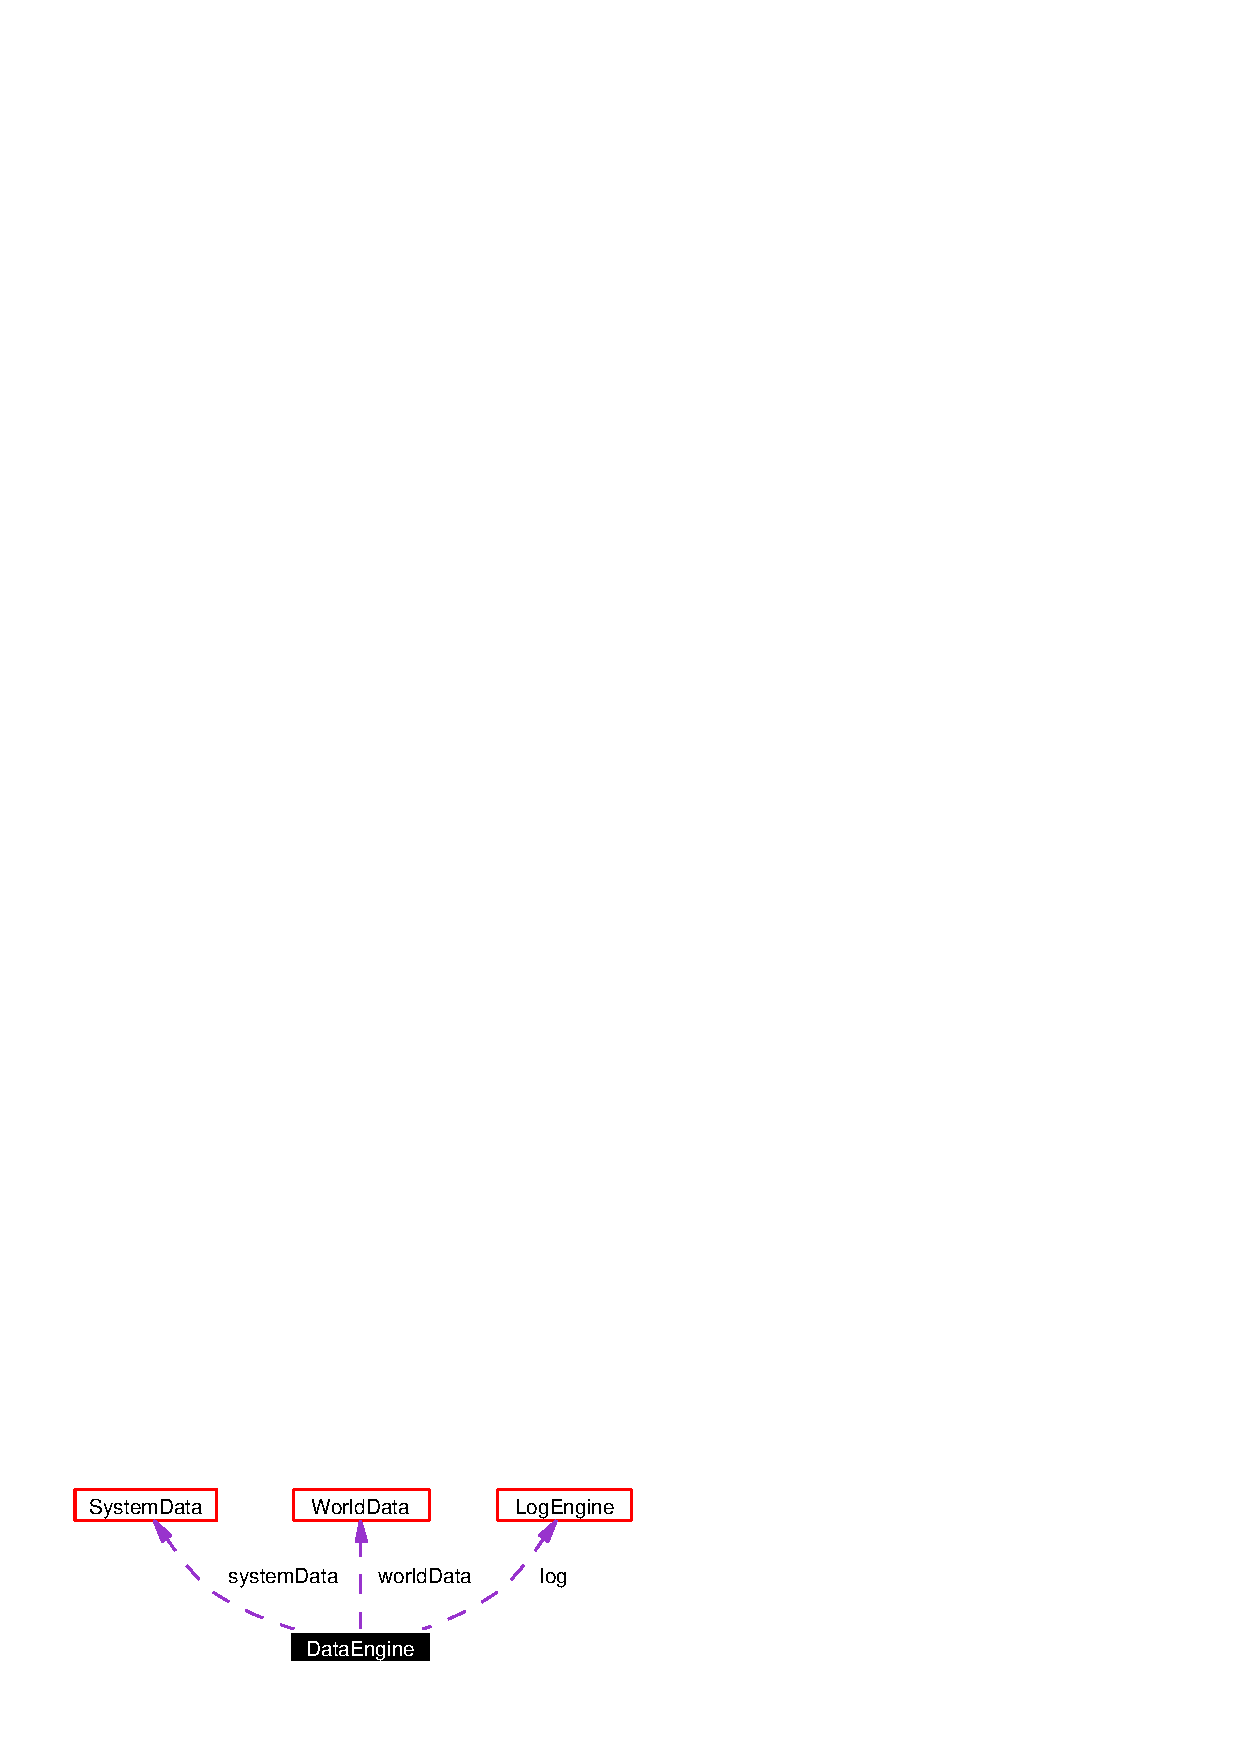
\includegraphics[width=152pt]{classDataEngine__coll__graph}
\end{center}
\end{figure}
\subsection*{Public Member Functions}
\begin{CompactItemize}
\item 
int {\bf start} ({\bf World\-Data} $\ast$wrl\-Data, {\bf System\-Data} $\ast$sys\-Data)
\item 
int {\bf load\-World\-Data} (void)
\item 
int {\bf unload\-World\-Data} (void)
\item 
int {\bf load\-System\-Data} (void)
\item 
int {\bf unload\-System\-Data} (void)
\item 
int {\bf stop} (void)
\end{CompactItemize}
\subsection*{Private Attributes}
\begin{CompactItemize}
\item 
{\bf Log\-Engine} {\bf log}
\item 
{\bf World\-Data} $\ast$ {\bf world\-Data}
\item 
{\bf System\-Data} $\ast$ {\bf system\-Data}
\end{CompactItemize}


\subsection{Member Function Documentation}
\index{DataEngine@{Data\-Engine}!loadSystemData@{loadSystemData}}
\index{loadSystemData@{loadSystemData}!DataEngine@{Data\-Engine}}
\subsubsection{\setlength{\rightskip}{0pt plus 5cm}int Data\-Engine::load\-System\-Data (void)}\label{classDataEngine_a3}


\index{DataEngine@{Data\-Engine}!loadWorldData@{loadWorldData}}
\index{loadWorldData@{loadWorldData}!DataEngine@{Data\-Engine}}
\subsubsection{\setlength{\rightskip}{0pt plus 5cm}int Data\-Engine::load\-World\-Data (void)}\label{classDataEngine_a1}


\index{DataEngine@{Data\-Engine}!start@{start}}
\index{start@{start}!DataEngine@{Data\-Engine}}
\subsubsection{\setlength{\rightskip}{0pt plus 5cm}int Data\-Engine::start ({\bf World\-Data} $\ast$ {\em wrl\-Data}, {\bf System\-Data} $\ast$ {\em sys\-Data})}\label{classDataEngine_a0}


\index{DataEngine@{Data\-Engine}!stop@{stop}}
\index{stop@{stop}!DataEngine@{Data\-Engine}}
\subsubsection{\setlength{\rightskip}{0pt plus 5cm}int Data\-Engine::stop (void)}\label{classDataEngine_a5}


\index{DataEngine@{Data\-Engine}!unloadSystemData@{unloadSystemData}}
\index{unloadSystemData@{unloadSystemData}!DataEngine@{Data\-Engine}}
\subsubsection{\setlength{\rightskip}{0pt plus 5cm}int Data\-Engine::unload\-System\-Data (void)}\label{classDataEngine_a4}


\index{DataEngine@{Data\-Engine}!unloadWorldData@{unloadWorldData}}
\index{unloadWorldData@{unloadWorldData}!DataEngine@{Data\-Engine}}
\subsubsection{\setlength{\rightskip}{0pt plus 5cm}int Data\-Engine::unload\-World\-Data (void)}\label{classDataEngine_a2}




\subsection{Member Data Documentation}
\index{DataEngine@{Data\-Engine}!log@{log}}
\index{log@{log}!DataEngine@{Data\-Engine}}
\subsubsection{\setlength{\rightskip}{0pt plus 5cm}{\bf Log\-Engine} {\bf Data\-Engine::log}\hspace{0.3cm}{\tt  [private]}}\label{classDataEngine_r0}


\index{DataEngine@{Data\-Engine}!systemData@{systemData}}
\index{systemData@{systemData}!DataEngine@{Data\-Engine}}
\subsubsection{\setlength{\rightskip}{0pt plus 5cm}{\bf System\-Data}$\ast$ {\bf Data\-Engine::system\-Data}\hspace{0.3cm}{\tt  [private]}}\label{classDataEngine_r2}


\index{DataEngine@{Data\-Engine}!worldData@{worldData}}
\index{worldData@{worldData}!DataEngine@{Data\-Engine}}
\subsubsection{\setlength{\rightskip}{0pt plus 5cm}{\bf World\-Data}$\ast$ {\bf Data\-Engine::world\-Data}\hspace{0.3cm}{\tt  [private]}}\label{classDataEngine_r1}




The documentation for this class was generated from the following files:\begin{CompactItemize}
\item 
src/data/{\bf data\-Engine.hpp}\item 
src/data/{\bf data\-Engine.cpp}\end{CompactItemize}

\section{Example\-Application Class Reference}
\label{classExampleApplication}\index{ExampleApplication@{ExampleApplication}}
{\tt \#include $<$Example\-Application.h$>$}

Collaboration diagram for Example\-Application:\begin{figure}[H]
\begin{center}
\leavevmode
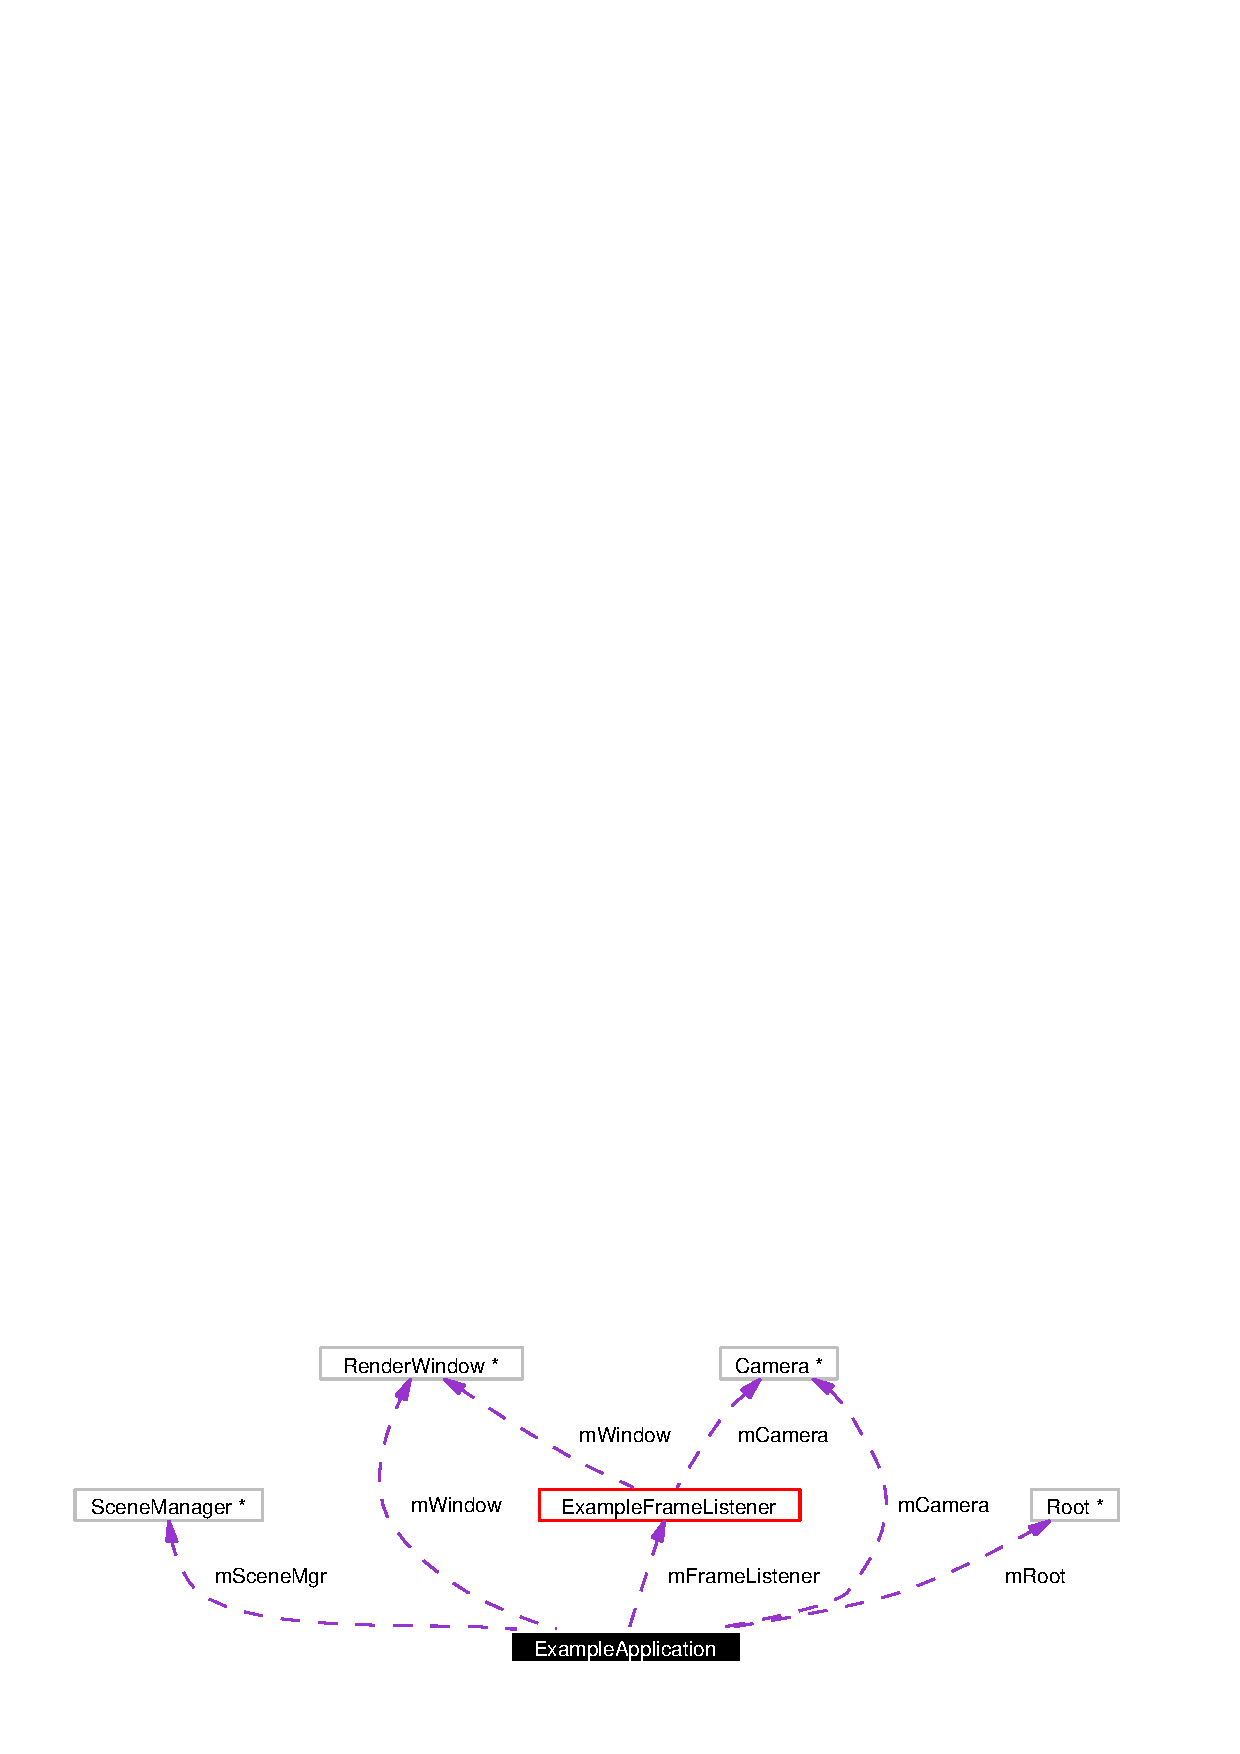
\includegraphics[width=280pt]{classExampleApplication__coll__graph}
\end{center}
\end{figure}
\subsection*{Public Member Functions}
\begin{CompactItemize}
\item 
{\bf Example\-Application} ()
\begin{CompactList}\small\item\em Standard constructor. \item\end{CompactList}\item 
void {\bf go} (int res\-X, int res\-Y)
\begin{CompactList}\small\item\em Start the example. \item\end{CompactList}\item 
{\bf $\sim$Example\-Application} ()
\begin{CompactList}\small\item\em Standard destructor. \item\end{CompactList}\item 
bool {\bf configure} (int res\-X, int res\-Y)
\item 
void {\bf choose\-Scene\-Manager} (void)
\item 
void {\bf create\-Camera} (void)
\item 
bool {\bf manual\-Initialize} (const String \&desired\-Renderer, int res\-X, int res\-Y)
\item 
void {\bf create\-Frame\-Listener} (void)
\item 
void {\bf create\-Scene} (void)
\item 
virtual void {\bf create\-Viewports} (void)
\item 
virtual void {\bf setup\-Resources} (void)
\begin{CompactList}\small\item\em Method which will define the source of resources (other than current folder). \item\end{CompactList}\end{CompactItemize}
\subsection*{Public Attributes}
\begin{CompactItemize}
\item 
Root $\ast$ {\bf m\-Root}
\item 
Camera $\ast$ {\bf m\-Camera}
\item 
Scene\-Manager $\ast$ {\bf m\-Scene\-Mgr}
\item 
{\bf Example\-Frame\-Listener} $\ast$ {\bf m\-Frame\-Listener}
\item 
Render\-Window $\ast$ {\bf m\-Window}
\end{CompactItemize}


\subsection{Detailed Description}
Base class which manages the standard startup of an {\bf Ogre}{\rm (p.\,\pageref{namespaceOgre})} application. Designed to be subclassed for specific examples if required. 



\subsection{Constructor \& Destructor Documentation}
\index{ExampleApplication@{Example\-Application}!ExampleApplication@{ExampleApplication}}
\index{ExampleApplication@{ExampleApplication}!ExampleApplication@{Example\-Application}}
\subsubsection{\setlength{\rightskip}{0pt plus 5cm}Example\-Application::Example\-Application ()\hspace{0.3cm}{\tt  [inline]}}\label{classExampleApplication_a0}


Standard constructor. 

\index{ExampleApplication@{Example\-Application}!~ExampleApplication@{$\sim$ExampleApplication}}
\index{~ExampleApplication@{$\sim$ExampleApplication}!ExampleApplication@{Example\-Application}}
\subsubsection{\setlength{\rightskip}{0pt plus 5cm}Example\-Application::$\sim${\bf Example\-Application} ()\hspace{0.3cm}{\tt  [inline]}}\label{classExampleApplication_a2}


Standard destructor. 



\subsection{Member Function Documentation}
\index{ExampleApplication@{Example\-Application}!chooseSceneManager@{chooseSceneManager}}
\index{chooseSceneManager@{chooseSceneManager}!ExampleApplication@{Example\-Application}}
\subsubsection{\setlength{\rightskip}{0pt plus 5cm}void Example\-Application::choose\-Scene\-Manager (void)\hspace{0.3cm}{\tt  [inline]}}\label{classExampleApplication_a4}


\index{ExampleApplication@{Example\-Application}!configure@{configure}}
\index{configure@{configure}!ExampleApplication@{Example\-Application}}
\subsubsection{\setlength{\rightskip}{0pt plus 5cm}bool Example\-Application::configure (int {\em res\-X}, int {\em res\-Y})\hspace{0.3cm}{\tt  [inline]}}\label{classExampleApplication_a3}


Configures the application - returns false if the user chooses to abandon configuration. \index{ExampleApplication@{Example\-Application}!createCamera@{createCamera}}
\index{createCamera@{createCamera}!ExampleApplication@{Example\-Application}}
\subsubsection{\setlength{\rightskip}{0pt plus 5cm}void Example\-Application::create\-Camera (void)\hspace{0.3cm}{\tt  [inline]}}\label{classExampleApplication_a5}


\index{ExampleApplication@{Example\-Application}!createFrameListener@{createFrameListener}}
\index{createFrameListener@{createFrameListener}!ExampleApplication@{Example\-Application}}
\subsubsection{\setlength{\rightskip}{0pt plus 5cm}void Example\-Application::create\-Frame\-Listener (void)\hspace{0.3cm}{\tt  [inline]}}\label{classExampleApplication_a7}


\index{ExampleApplication@{Example\-Application}!createScene@{createScene}}
\index{createScene@{createScene}!ExampleApplication@{Example\-Application}}
\subsubsection{\setlength{\rightskip}{0pt plus 5cm}void Example\-Application::create\-Scene (void)\hspace{0.3cm}{\tt  [inline]}}\label{classExampleApplication_a8}


\index{ExampleApplication@{Example\-Application}!createViewports@{createViewports}}
\index{createViewports@{createViewports}!ExampleApplication@{Example\-Application}}
\subsubsection{\setlength{\rightskip}{0pt plus 5cm}virtual void Example\-Application::create\-Viewports (void)\hspace{0.3cm}{\tt  [inline, virtual]}}\label{classExampleApplication_a9}


\index{ExampleApplication@{Example\-Application}!go@{go}}
\index{go@{go}!ExampleApplication@{Example\-Application}}
\subsubsection{\setlength{\rightskip}{0pt plus 5cm}void Example\-Application::go (int {\em res\-X}, int {\em res\-Y})\hspace{0.3cm}{\tt  [inline]}}\label{classExampleApplication_a1}


Start the example. 

\index{ExampleApplication@{Example\-Application}!manualInitialize@{manualInitialize}}
\index{manualInitialize@{manualInitialize}!ExampleApplication@{Example\-Application}}
\subsubsection{\setlength{\rightskip}{0pt plus 5cm}bool Example\-Application::manual\-Initialize (const String \& {\em desired\-Renderer}, int {\em res\-X}, int {\em res\-Y})\hspace{0.3cm}{\tt  [inline]}}\label{classExampleApplication_a6}


\index{ExampleApplication@{Example\-Application}!setupResources@{setupResources}}
\index{setupResources@{setupResources}!ExampleApplication@{Example\-Application}}
\subsubsection{\setlength{\rightskip}{0pt plus 5cm}virtual void Example\-Application::setup\-Resources (void)\hspace{0.3cm}{\tt  [inline, virtual]}}\label{classExampleApplication_a10}


Method which will define the source of resources (other than current folder). 



\subsection{Member Data Documentation}
\index{ExampleApplication@{Example\-Application}!mCamera@{mCamera}}
\index{mCamera@{mCamera}!ExampleApplication@{Example\-Application}}
\subsubsection{\setlength{\rightskip}{0pt plus 5cm}Camera$\ast$ {\bf Example\-Application::m\-Camera}}\label{classExampleApplication_o1}


\index{ExampleApplication@{Example\-Application}!mFrameListener@{mFrameListener}}
\index{mFrameListener@{mFrameListener}!ExampleApplication@{Example\-Application}}
\subsubsection{\setlength{\rightskip}{0pt plus 5cm}{\bf Example\-Frame\-Listener}$\ast$ {\bf Example\-Application::m\-Frame\-Listener}}\label{classExampleApplication_o3}


\index{ExampleApplication@{Example\-Application}!mRoot@{mRoot}}
\index{mRoot@{mRoot}!ExampleApplication@{Example\-Application}}
\subsubsection{\setlength{\rightskip}{0pt plus 5cm}Root$\ast$ {\bf Example\-Application::m\-Root}}\label{classExampleApplication_o0}


\index{ExampleApplication@{Example\-Application}!mSceneMgr@{mSceneMgr}}
\index{mSceneMgr@{mSceneMgr}!ExampleApplication@{Example\-Application}}
\subsubsection{\setlength{\rightskip}{0pt plus 5cm}Scene\-Manager$\ast$ {\bf Example\-Application::m\-Scene\-Mgr}}\label{classExampleApplication_o2}


\index{ExampleApplication@{Example\-Application}!mWindow@{mWindow}}
\index{mWindow@{mWindow}!ExampleApplication@{Example\-Application}}
\subsubsection{\setlength{\rightskip}{0pt plus 5cm}Render\-Window$\ast$ {\bf Example\-Application::m\-Window}}\label{classExampleApplication_o4}




The documentation for this class was generated from the following file:\begin{CompactItemize}
\item 
src/graphics/{\bf Example\-Application.h}\end{CompactItemize}

\section{Example\-Frame\-Listener Class Reference}
\label{classExampleFrameListener}\index{ExampleFrameListener@{ExampleFrameListener}}
{\tt \#include $<$Example\-Frame\-Listener.h$>$}

Inheritance diagram for Example\-Frame\-Listener::\begin{figure}[H]
\begin{center}
\leavevmode
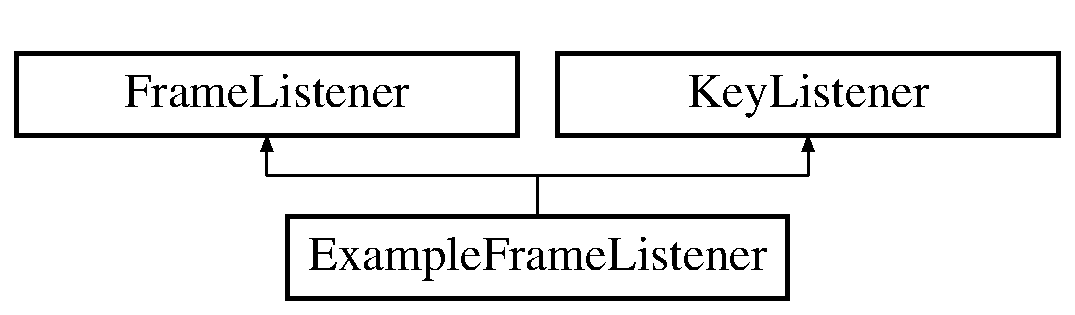
\includegraphics[height=2cm]{classExampleFrameListener}
\end{center}
\end{figure}
Collaboration diagram for Example\-Frame\-Listener:\begin{figure}[H]
\begin{center}
\leavevmode
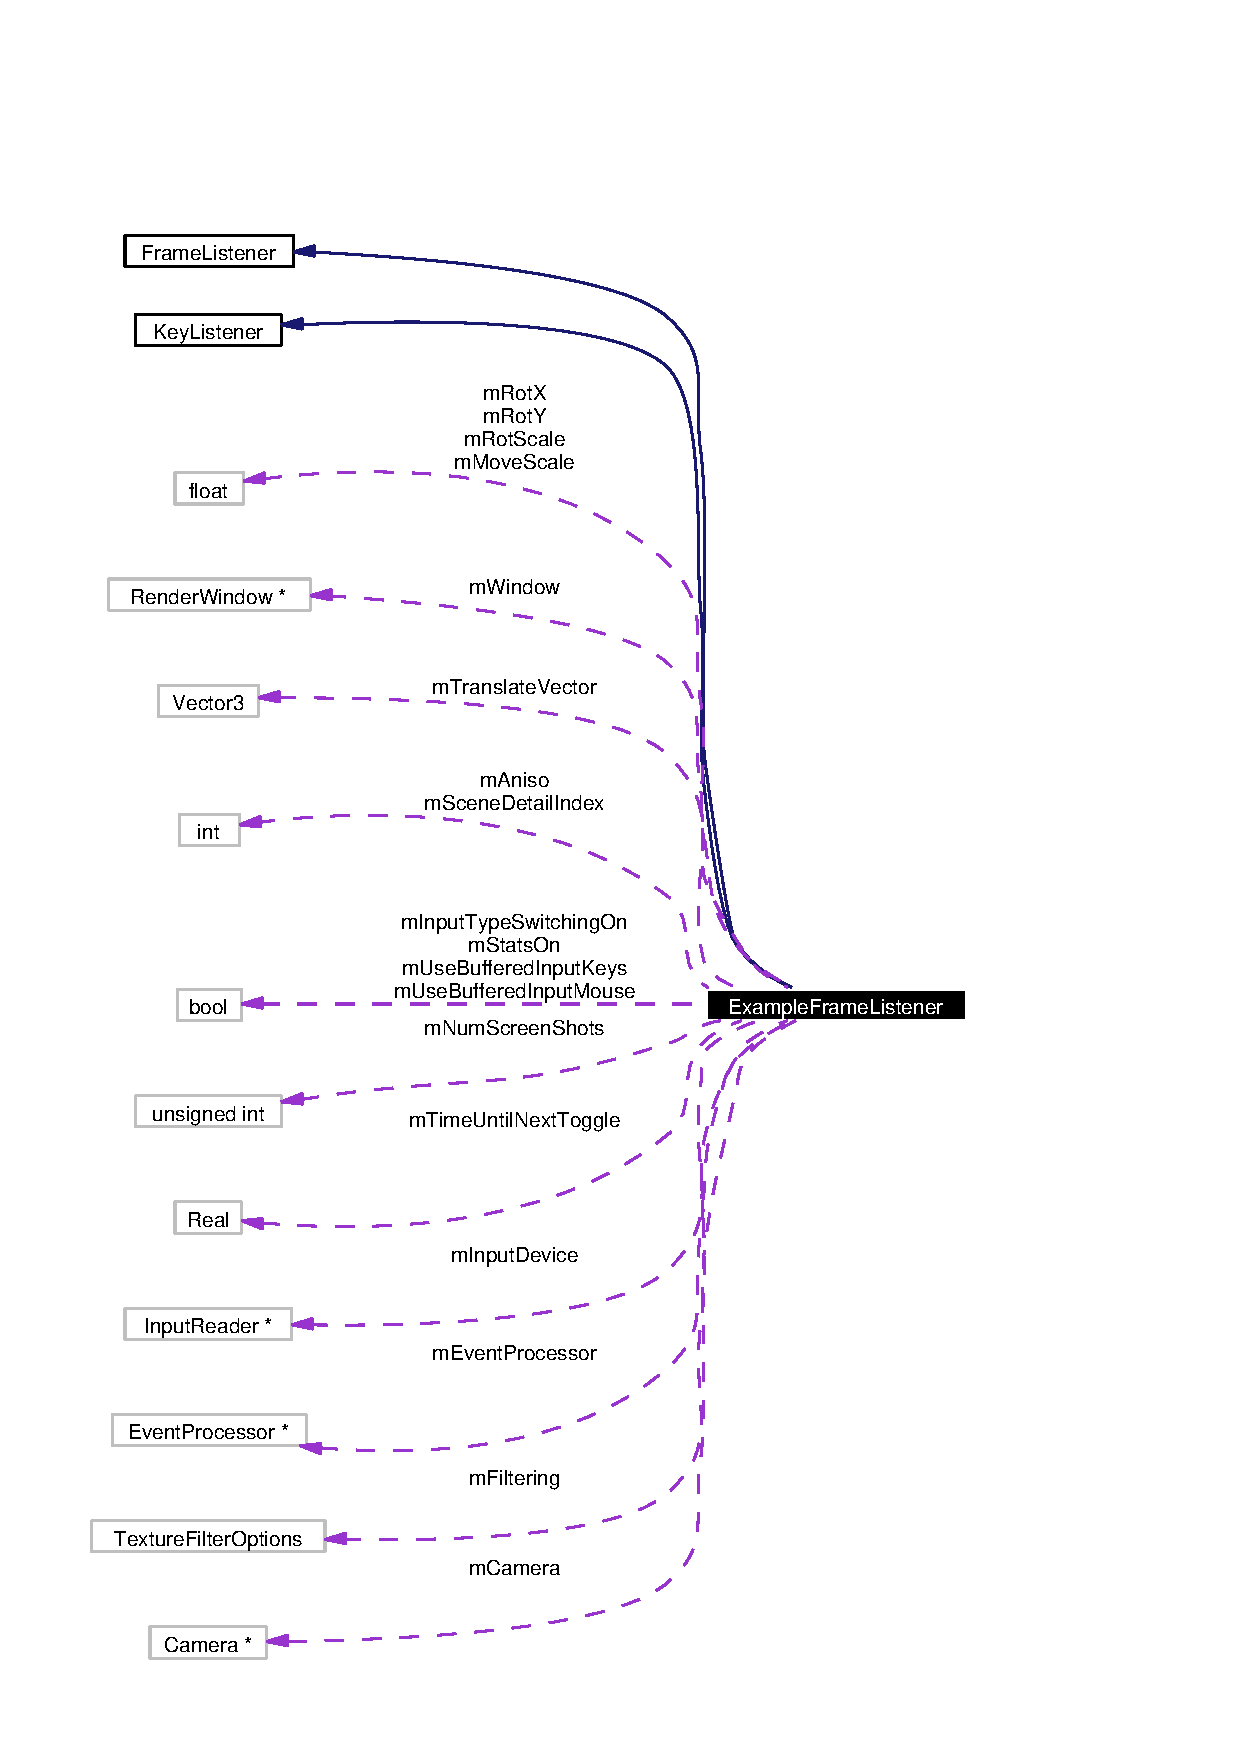
\includegraphics[width=236pt]{classExampleFrameListener__coll__graph}
\end{center}
\end{figure}
\subsection*{Public Member Functions}
\begin{CompactItemize}
\item 
{\bf Example\-Frame\-Listener} (Render\-Window $\ast$win, Camera $\ast$cam, bool use\-Buffered\-Input\-Keys=false, bool use\-Buffered\-Input\-Mouse=false)
\item 
virtual {\bf $\sim$Example\-Frame\-Listener} ()
\item 
virtual bool {\bf process\-Unbuffered\-Key\-Input} (const Frame\-Event \&evt)
\item 
bool {\bf process\-Unbuffered\-Mouse\-Input} (const Frame\-Event \&evt)
\item 
void {\bf move\-Camera} ()
\item 
void {\bf show\-Debug\-Overlay} (bool show)
\item 
bool {\bf frame\-Started} (const Frame\-Event \&evt)
\item 
bool {\bf frame\-Ended} (const Frame\-Event \&evt)
\item 
void {\bf switch\-Mouse\-Mode} ()
\item 
void {\bf switch\-Key\-Mode} ()
\item 
void {\bf key\-Clicked} (Key\-Event $\ast$e)
\item 
void {\bf key\-Pressed} (Key\-Event $\ast$e)
\item 
void {\bf key\-Released} (Key\-Event $\ast$e)
\end{CompactItemize}
\subsection*{Protected Attributes}
\begin{CompactItemize}
\item 
Event\-Processor $\ast$ {\bf m\-Event\-Processor}
\item 
Input\-Reader $\ast$ {\bf m\-Input\-Device}
\item 
Camera $\ast$ {\bf m\-Camera}
\item 
Vector3 {\bf m\-Translate\-Vector}
\item 
Render\-Window $\ast$ {\bf m\-Window}
\item 
bool {\bf m\-Stats\-On}
\item 
bool {\bf m\-Use\-Buffered\-Input\-Keys}
\item 
bool {\bf m\-Use\-Buffered\-Input\-Mouse}
\item 
bool {\bf m\-Input\-Type\-Switching\-On}
\item 
unsigned int {\bf m\-Num\-Screen\-Shots}
\item 
float {\bf m\-Move\-Scale}
\item 
float {\bf m\-Rot\-Scale}
\item 
Real {\bf m\-Time\-Until\-Next\-Toggle}
\item 
float {\bf m\-Rot\-X}
\item 
float {\bf m\-Rot\-Y}
\item 
Texture\-Filter\-Options {\bf m\-Filtering}
\item 
int {\bf m\-Aniso}
\end{CompactItemize}
\subsection*{Private Member Functions}
\begin{CompactItemize}
\item 
void {\bf update\-Stats} (void)
\end{CompactItemize}
\subsection*{Private Attributes}
\begin{CompactItemize}
\item 
int {\bf m\-Scene\-Detail\-Index}
\end{CompactItemize}


\subsection{Constructor \& Destructor Documentation}
\index{ExampleFrameListener@{Example\-Frame\-Listener}!ExampleFrameListener@{ExampleFrameListener}}
\index{ExampleFrameListener@{ExampleFrameListener}!ExampleFrameListener@{Example\-Frame\-Listener}}
\subsubsection{\setlength{\rightskip}{0pt plus 5cm}Example\-Frame\-Listener::Example\-Frame\-Listener (Render\-Window $\ast$ {\em win}, Camera $\ast$ {\em cam}, bool {\em use\-Buffered\-Input\-Keys} = false, bool {\em use\-Buffered\-Input\-Mouse} = false)\hspace{0.3cm}{\tt  [inline]}}\label{classExampleFrameListener_a0}


\index{ExampleFrameListener@{Example\-Frame\-Listener}!~ExampleFrameListener@{$\sim$ExampleFrameListener}}
\index{~ExampleFrameListener@{$\sim$ExampleFrameListener}!ExampleFrameListener@{Example\-Frame\-Listener}}
\subsubsection{\setlength{\rightskip}{0pt plus 5cm}virtual Example\-Frame\-Listener::$\sim${\bf Example\-Frame\-Listener} ()\hspace{0.3cm}{\tt  [inline, virtual]}}\label{classExampleFrameListener_a1}




\subsection{Member Function Documentation}
\index{ExampleFrameListener@{Example\-Frame\-Listener}!frameEnded@{frameEnded}}
\index{frameEnded@{frameEnded}!ExampleFrameListener@{Example\-Frame\-Listener}}
\subsubsection{\setlength{\rightskip}{0pt plus 5cm}bool Example\-Frame\-Listener::frame\-Ended (const Frame\-Event \& {\em evt})\hspace{0.3cm}{\tt  [inline]}}\label{classExampleFrameListener_a7}


\index{ExampleFrameListener@{Example\-Frame\-Listener}!frameStarted@{frameStarted}}
\index{frameStarted@{frameStarted}!ExampleFrameListener@{Example\-Frame\-Listener}}
\subsubsection{\setlength{\rightskip}{0pt plus 5cm}bool Example\-Frame\-Listener::frame\-Started (const Frame\-Event \& {\em evt})\hspace{0.3cm}{\tt  [inline]}}\label{classExampleFrameListener_a6}


\index{ExampleFrameListener@{Example\-Frame\-Listener}!keyClicked@{keyClicked}}
\index{keyClicked@{keyClicked}!ExampleFrameListener@{Example\-Frame\-Listener}}
\subsubsection{\setlength{\rightskip}{0pt plus 5cm}void Example\-Frame\-Listener::key\-Clicked (Key\-Event $\ast$ {\em e})\hspace{0.3cm}{\tt  [inline]}}\label{classExampleFrameListener_a10}


\index{ExampleFrameListener@{Example\-Frame\-Listener}!keyPressed@{keyPressed}}
\index{keyPressed@{keyPressed}!ExampleFrameListener@{Example\-Frame\-Listener}}
\subsubsection{\setlength{\rightskip}{0pt plus 5cm}void Example\-Frame\-Listener::key\-Pressed (Key\-Event $\ast$ {\em e})\hspace{0.3cm}{\tt  [inline]}}\label{classExampleFrameListener_a11}


\index{ExampleFrameListener@{Example\-Frame\-Listener}!keyReleased@{keyReleased}}
\index{keyReleased@{keyReleased}!ExampleFrameListener@{Example\-Frame\-Listener}}
\subsubsection{\setlength{\rightskip}{0pt plus 5cm}void Example\-Frame\-Listener::key\-Released (Key\-Event $\ast$ {\em e})\hspace{0.3cm}{\tt  [inline]}}\label{classExampleFrameListener_a12}


\index{ExampleFrameListener@{Example\-Frame\-Listener}!moveCamera@{moveCamera}}
\index{moveCamera@{moveCamera}!ExampleFrameListener@{Example\-Frame\-Listener}}
\subsubsection{\setlength{\rightskip}{0pt plus 5cm}void Example\-Frame\-Listener::move\-Camera ()\hspace{0.3cm}{\tt  [inline]}}\label{classExampleFrameListener_a4}


\index{ExampleFrameListener@{Example\-Frame\-Listener}!processUnbufferedKeyInput@{processUnbufferedKeyInput}}
\index{processUnbufferedKeyInput@{processUnbufferedKeyInput}!ExampleFrameListener@{Example\-Frame\-Listener}}
\subsubsection{\setlength{\rightskip}{0pt plus 5cm}virtual bool Example\-Frame\-Listener::process\-Unbuffered\-Key\-Input (const Frame\-Event \& {\em evt})\hspace{0.3cm}{\tt  [inline, virtual]}}\label{classExampleFrameListener_a2}


\index{ExampleFrameListener@{Example\-Frame\-Listener}!processUnbufferedMouseInput@{processUnbufferedMouseInput}}
\index{processUnbufferedMouseInput@{processUnbufferedMouseInput}!ExampleFrameListener@{Example\-Frame\-Listener}}
\subsubsection{\setlength{\rightskip}{0pt plus 5cm}bool Example\-Frame\-Listener::process\-Unbuffered\-Mouse\-Input (const Frame\-Event \& {\em evt})\hspace{0.3cm}{\tt  [inline]}}\label{classExampleFrameListener_a3}


\index{ExampleFrameListener@{Example\-Frame\-Listener}!showDebugOverlay@{showDebugOverlay}}
\index{showDebugOverlay@{showDebugOverlay}!ExampleFrameListener@{Example\-Frame\-Listener}}
\subsubsection{\setlength{\rightskip}{0pt plus 5cm}void Example\-Frame\-Listener::show\-Debug\-Overlay (bool {\em show})\hspace{0.3cm}{\tt  [inline]}}\label{classExampleFrameListener_a5}


\index{ExampleFrameListener@{Example\-Frame\-Listener}!switchKeyMode@{switchKeyMode}}
\index{switchKeyMode@{switchKeyMode}!ExampleFrameListener@{Example\-Frame\-Listener}}
\subsubsection{\setlength{\rightskip}{0pt plus 5cm}void Example\-Frame\-Listener::switch\-Key\-Mode ()\hspace{0.3cm}{\tt  [inline]}}\label{classExampleFrameListener_a9}


\index{ExampleFrameListener@{Example\-Frame\-Listener}!switchMouseMode@{switchMouseMode}}
\index{switchMouseMode@{switchMouseMode}!ExampleFrameListener@{Example\-Frame\-Listener}}
\subsubsection{\setlength{\rightskip}{0pt plus 5cm}void Example\-Frame\-Listener::switch\-Mouse\-Mode ()\hspace{0.3cm}{\tt  [inline]}}\label{classExampleFrameListener_a8}


\index{ExampleFrameListener@{Example\-Frame\-Listener}!updateStats@{updateStats}}
\index{updateStats@{updateStats}!ExampleFrameListener@{Example\-Frame\-Listener}}
\subsubsection{\setlength{\rightskip}{0pt plus 5cm}void Example\-Frame\-Listener::update\-Stats (void)\hspace{0.3cm}{\tt  [inline, private]}}\label{classExampleFrameListener_d0}




\subsection{Member Data Documentation}
\index{ExampleFrameListener@{Example\-Frame\-Listener}!mAniso@{mAniso}}
\index{mAniso@{mAniso}!ExampleFrameListener@{Example\-Frame\-Listener}}
\subsubsection{\setlength{\rightskip}{0pt plus 5cm}int {\bf Example\-Frame\-Listener::m\-Aniso}\hspace{0.3cm}{\tt  [protected]}}\label{classExampleFrameListener_p16}


\index{ExampleFrameListener@{Example\-Frame\-Listener}!mCamera@{mCamera}}
\index{mCamera@{mCamera}!ExampleFrameListener@{Example\-Frame\-Listener}}
\subsubsection{\setlength{\rightskip}{0pt plus 5cm}Camera$\ast$ {\bf Example\-Frame\-Listener::m\-Camera}\hspace{0.3cm}{\tt  [protected]}}\label{classExampleFrameListener_p2}


\index{ExampleFrameListener@{Example\-Frame\-Listener}!mEventProcessor@{mEventProcessor}}
\index{mEventProcessor@{mEventProcessor}!ExampleFrameListener@{Example\-Frame\-Listener}}
\subsubsection{\setlength{\rightskip}{0pt plus 5cm}Event\-Processor$\ast$ {\bf Example\-Frame\-Listener::m\-Event\-Processor}\hspace{0.3cm}{\tt  [protected]}}\label{classExampleFrameListener_p0}


\index{ExampleFrameListener@{Example\-Frame\-Listener}!mFiltering@{mFiltering}}
\index{mFiltering@{mFiltering}!ExampleFrameListener@{Example\-Frame\-Listener}}
\subsubsection{\setlength{\rightskip}{0pt plus 5cm}Texture\-Filter\-Options {\bf Example\-Frame\-Listener::m\-Filtering}\hspace{0.3cm}{\tt  [protected]}}\label{classExampleFrameListener_p15}


\index{ExampleFrameListener@{Example\-Frame\-Listener}!mInputDevice@{mInputDevice}}
\index{mInputDevice@{mInputDevice}!ExampleFrameListener@{Example\-Frame\-Listener}}
\subsubsection{\setlength{\rightskip}{0pt plus 5cm}Input\-Reader$\ast$ {\bf Example\-Frame\-Listener::m\-Input\-Device}\hspace{0.3cm}{\tt  [protected]}}\label{classExampleFrameListener_p1}


\index{ExampleFrameListener@{Example\-Frame\-Listener}!mInputTypeSwitchingOn@{mInputTypeSwitchingOn}}
\index{mInputTypeSwitchingOn@{mInputTypeSwitchingOn}!ExampleFrameListener@{Example\-Frame\-Listener}}
\subsubsection{\setlength{\rightskip}{0pt plus 5cm}bool {\bf Example\-Frame\-Listener::m\-Input\-Type\-Switching\-On}\hspace{0.3cm}{\tt  [protected]}}\label{classExampleFrameListener_p8}


\index{ExampleFrameListener@{Example\-Frame\-Listener}!mMoveScale@{mMoveScale}}
\index{mMoveScale@{mMoveScale}!ExampleFrameListener@{Example\-Frame\-Listener}}
\subsubsection{\setlength{\rightskip}{0pt plus 5cm}float {\bf Example\-Frame\-Listener::m\-Move\-Scale}\hspace{0.3cm}{\tt  [protected]}}\label{classExampleFrameListener_p10}


\index{ExampleFrameListener@{Example\-Frame\-Listener}!mNumScreenShots@{mNumScreenShots}}
\index{mNumScreenShots@{mNumScreenShots}!ExampleFrameListener@{Example\-Frame\-Listener}}
\subsubsection{\setlength{\rightskip}{0pt plus 5cm}unsigned int {\bf Example\-Frame\-Listener::m\-Num\-Screen\-Shots}\hspace{0.3cm}{\tt  [protected]}}\label{classExampleFrameListener_p9}


\index{ExampleFrameListener@{Example\-Frame\-Listener}!mRotScale@{mRotScale}}
\index{mRotScale@{mRotScale}!ExampleFrameListener@{Example\-Frame\-Listener}}
\subsubsection{\setlength{\rightskip}{0pt plus 5cm}float {\bf Example\-Frame\-Listener::m\-Rot\-Scale}\hspace{0.3cm}{\tt  [protected]}}\label{classExampleFrameListener_p11}


\index{ExampleFrameListener@{Example\-Frame\-Listener}!mRotX@{mRotX}}
\index{mRotX@{mRotX}!ExampleFrameListener@{Example\-Frame\-Listener}}
\subsubsection{\setlength{\rightskip}{0pt plus 5cm}float {\bf Example\-Frame\-Listener::m\-Rot\-X}\hspace{0.3cm}{\tt  [protected]}}\label{classExampleFrameListener_p13}


\index{ExampleFrameListener@{Example\-Frame\-Listener}!mRotY@{mRotY}}
\index{mRotY@{mRotY}!ExampleFrameListener@{Example\-Frame\-Listener}}
\subsubsection{\setlength{\rightskip}{0pt plus 5cm}float {\bf Example\-Frame\-Listener::m\-Rot\-Y}\hspace{0.3cm}{\tt  [protected]}}\label{classExampleFrameListener_p14}


\index{ExampleFrameListener@{Example\-Frame\-Listener}!mSceneDetailIndex@{mSceneDetailIndex}}
\index{mSceneDetailIndex@{mSceneDetailIndex}!ExampleFrameListener@{Example\-Frame\-Listener}}
\subsubsection{\setlength{\rightskip}{0pt plus 5cm}int {\bf Example\-Frame\-Listener::m\-Scene\-Detail\-Index}\hspace{0.3cm}{\tt  [private]}}\label{classExampleFrameListener_r0}


\index{ExampleFrameListener@{Example\-Frame\-Listener}!mStatsOn@{mStatsOn}}
\index{mStatsOn@{mStatsOn}!ExampleFrameListener@{Example\-Frame\-Listener}}
\subsubsection{\setlength{\rightskip}{0pt plus 5cm}bool {\bf Example\-Frame\-Listener::m\-Stats\-On}\hspace{0.3cm}{\tt  [protected]}}\label{classExampleFrameListener_p5}


\index{ExampleFrameListener@{Example\-Frame\-Listener}!mTimeUntilNextToggle@{mTimeUntilNextToggle}}
\index{mTimeUntilNextToggle@{mTimeUntilNextToggle}!ExampleFrameListener@{Example\-Frame\-Listener}}
\subsubsection{\setlength{\rightskip}{0pt plus 5cm}Real {\bf Example\-Frame\-Listener::m\-Time\-Until\-Next\-Toggle}\hspace{0.3cm}{\tt  [protected]}}\label{classExampleFrameListener_p12}


\index{ExampleFrameListener@{Example\-Frame\-Listener}!mTranslateVector@{mTranslateVector}}
\index{mTranslateVector@{mTranslateVector}!ExampleFrameListener@{Example\-Frame\-Listener}}
\subsubsection{\setlength{\rightskip}{0pt plus 5cm}Vector3 {\bf Example\-Frame\-Listener::m\-Translate\-Vector}\hspace{0.3cm}{\tt  [protected]}}\label{classExampleFrameListener_p3}


\index{ExampleFrameListener@{Example\-Frame\-Listener}!mUseBufferedInputKeys@{mUseBufferedInputKeys}}
\index{mUseBufferedInputKeys@{mUseBufferedInputKeys}!ExampleFrameListener@{Example\-Frame\-Listener}}
\subsubsection{\setlength{\rightskip}{0pt plus 5cm}bool {\bf Example\-Frame\-Listener::m\-Use\-Buffered\-Input\-Keys}\hspace{0.3cm}{\tt  [protected]}}\label{classExampleFrameListener_p6}


\index{ExampleFrameListener@{Example\-Frame\-Listener}!mUseBufferedInputMouse@{mUseBufferedInputMouse}}
\index{mUseBufferedInputMouse@{mUseBufferedInputMouse}!ExampleFrameListener@{Example\-Frame\-Listener}}
\subsubsection{\setlength{\rightskip}{0pt plus 5cm}bool {\bf Example\-Frame\-Listener::m\-Use\-Buffered\-Input\-Mouse}\hspace{0.3cm}{\tt  [protected]}}\label{classExampleFrameListener_p7}


\index{ExampleFrameListener@{Example\-Frame\-Listener}!mWindow@{mWindow}}
\index{mWindow@{mWindow}!ExampleFrameListener@{Example\-Frame\-Listener}}
\subsubsection{\setlength{\rightskip}{0pt plus 5cm}Render\-Window$\ast$ {\bf Example\-Frame\-Listener::m\-Window}\hspace{0.3cm}{\tt  [protected]}}\label{classExampleFrameListener_p4}




The documentation for this class was generated from the following file:\begin{CompactItemize}
\item 
src/graphics/{\bf Example\-Frame\-Listener.h}\end{CompactItemize}

\section{Frame\-Listener Class Reference}
\label{classFrameListener}\index{FrameListener@{FrameListener}}
Inheritance diagram for Frame\-Listener::\begin{figure}[H]
\begin{center}
\leavevmode
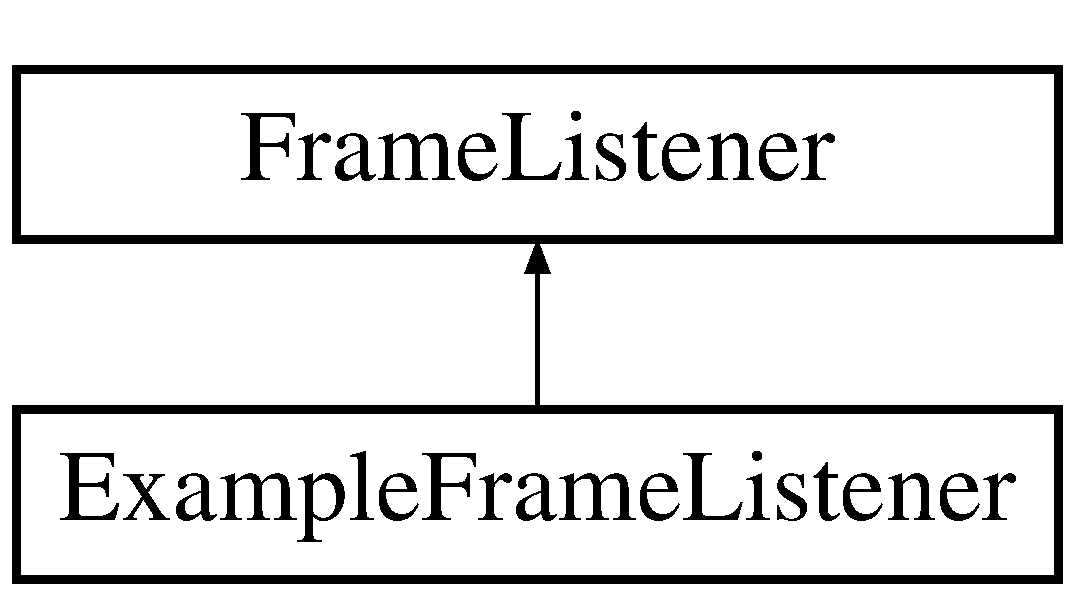
\includegraphics[height=2cm]{classFrameListener}
\end{center}
\end{figure}


The documentation for this class was generated from the following file:\begin{CompactItemize}
\item 
src/graphics/{\bf Example\-Frame\-Listener.h}\end{CompactItemize}

\section{Graphics\-Data Struct Reference}
\label{structGraphicsData}\index{GraphicsData@{GraphicsData}}
{\tt \#include $<$system.hpp$>$}

Collaboration diagram for Graphics\-Data:\begin{figure}[H]
\begin{center}
\leavevmode
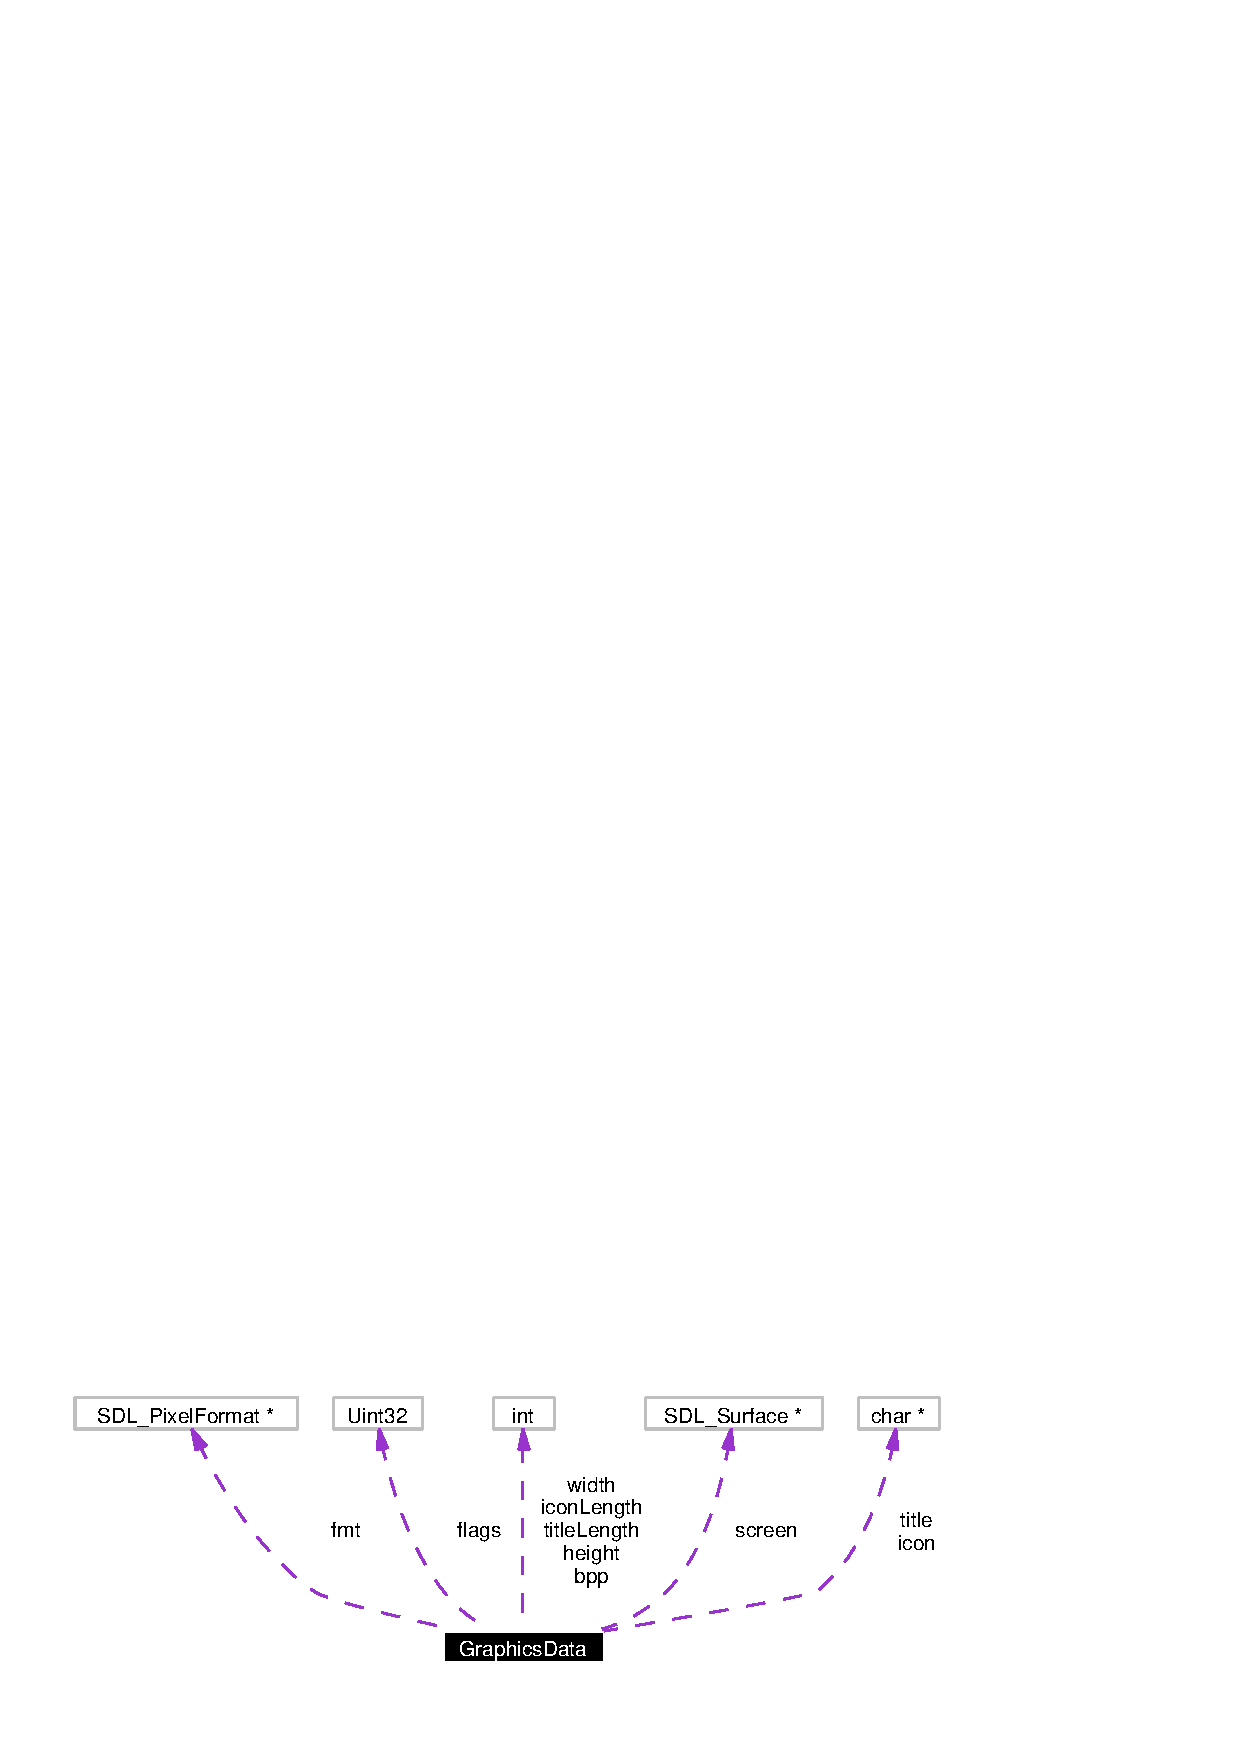
\includegraphics[width=231pt]{structGraphicsData__coll__graph}
\end{center}
\end{figure}
\subsection*{Public Attributes}
\begin{CompactItemize}
\item 
SDL\_\-Surface $\ast$ {\bf screen}
\item 
SDL\_\-Pixel\-Format $\ast$ {\bf fmt}
\item 
int {\bf width}
\item 
int {\bf height}
\item 
int {\bf bpp}
\item 
Uint32 {\bf flags}
\item 
char $\ast$ {\bf title}
\item 
char $\ast$ {\bf icon}
\item 
int {\bf title\-Length}
\item 
int {\bf icon\-Length}
\end{CompactItemize}


\subsection{Member Data Documentation}
\index{GraphicsData@{Graphics\-Data}!bpp@{bpp}}
\index{bpp@{bpp}!GraphicsData@{Graphics\-Data}}
\subsubsection{\setlength{\rightskip}{0pt plus 5cm}int {\bf Graphics\-Data::bpp}}\label{structGraphicsData_o4}


\index{GraphicsData@{Graphics\-Data}!flags@{flags}}
\index{flags@{flags}!GraphicsData@{Graphics\-Data}}
\subsubsection{\setlength{\rightskip}{0pt plus 5cm}Uint32 {\bf Graphics\-Data::flags}}\label{structGraphicsData_o5}


\index{GraphicsData@{Graphics\-Data}!fmt@{fmt}}
\index{fmt@{fmt}!GraphicsData@{Graphics\-Data}}
\subsubsection{\setlength{\rightskip}{0pt plus 5cm}SDL\_\-Pixel\-Format$\ast$ {\bf Graphics\-Data::fmt}}\label{structGraphicsData_o1}


\index{GraphicsData@{Graphics\-Data}!height@{height}}
\index{height@{height}!GraphicsData@{Graphics\-Data}}
\subsubsection{\setlength{\rightskip}{0pt plus 5cm}int {\bf Graphics\-Data::height}}\label{structGraphicsData_o3}


\index{GraphicsData@{Graphics\-Data}!icon@{icon}}
\index{icon@{icon}!GraphicsData@{Graphics\-Data}}
\subsubsection{\setlength{\rightskip}{0pt plus 5cm}char$\ast$ {\bf Graphics\-Data::icon}}\label{structGraphicsData_o7}


\index{GraphicsData@{Graphics\-Data}!iconLength@{iconLength}}
\index{iconLength@{iconLength}!GraphicsData@{Graphics\-Data}}
\subsubsection{\setlength{\rightskip}{0pt plus 5cm}int {\bf Graphics\-Data::icon\-Length}}\label{structGraphicsData_o9}


\index{GraphicsData@{Graphics\-Data}!screen@{screen}}
\index{screen@{screen}!GraphicsData@{Graphics\-Data}}
\subsubsection{\setlength{\rightskip}{0pt plus 5cm}SDL\_\-Surface$\ast$ {\bf Graphics\-Data::screen}}\label{structGraphicsData_o0}


\index{GraphicsData@{Graphics\-Data}!title@{title}}
\index{title@{title}!GraphicsData@{Graphics\-Data}}
\subsubsection{\setlength{\rightskip}{0pt plus 5cm}char$\ast$ {\bf Graphics\-Data::title}}\label{structGraphicsData_o6}


\index{GraphicsData@{Graphics\-Data}!titleLength@{titleLength}}
\index{titleLength@{titleLength}!GraphicsData@{Graphics\-Data}}
\subsubsection{\setlength{\rightskip}{0pt plus 5cm}int {\bf Graphics\-Data::title\-Length}}\label{structGraphicsData_o8}


\index{GraphicsData@{Graphics\-Data}!width@{width}}
\index{width@{width}!GraphicsData@{Graphics\-Data}}
\subsubsection{\setlength{\rightskip}{0pt plus 5cm}int {\bf Graphics\-Data::width}}\label{structGraphicsData_o2}




The documentation for this struct was generated from the following file:\begin{CompactItemize}
\item 
src/{\bf system.hpp}\end{CompactItemize}

\section{Graphics\-Engine Class Reference}
\label{classGraphicsEngine}\index{GraphicsEngine@{GraphicsEngine}}
{\tt \#include $<$graphics\-Engine.hpp$>$}

Collaboration diagram for Graphics\-Engine:\begin{figure}[H]
\begin{center}
\leavevmode
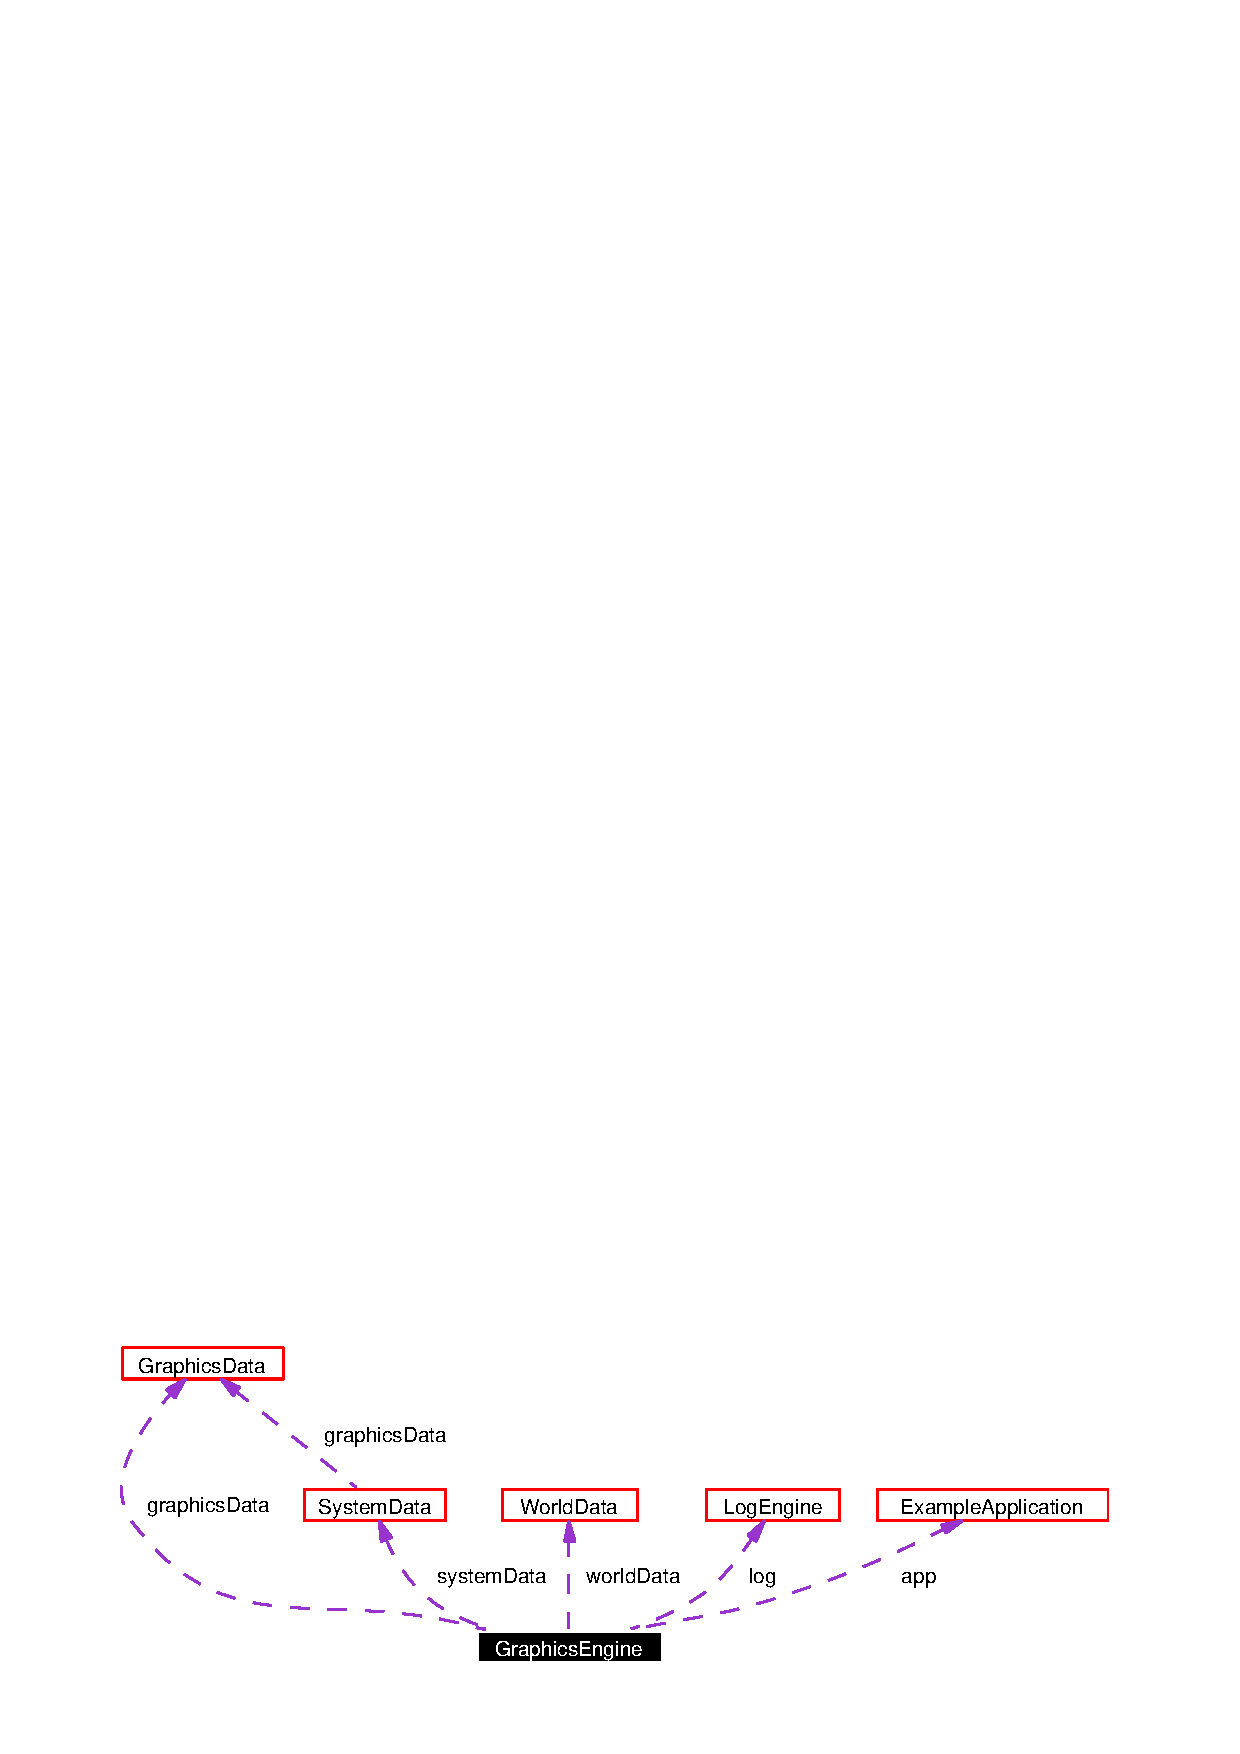
\includegraphics[width=266pt]{classGraphicsEngine__coll__graph}
\end{center}
\end{figure}
\subsection*{Public Member Functions}
\begin{CompactItemize}
\item 
int {\bf start} ({\bf World\-Data} $\ast$wrl\-Data, {\bf System\-Data} $\ast$sys\-Data)
\item 
int {\bf step} (void)
\item 
int {\bf stop} (void)
\end{CompactItemize}
\subsection*{Private Attributes}
\begin{CompactItemize}
\item 
{\bf Log\-Engine} {\bf log}
\item 
{\bf Graphics\-Data} $\ast$ {\bf graphics\-Data}
\item 
{\bf World\-Data} $\ast$ {\bf world\-Data}
\item 
{\bf System\-Data} $\ast$ {\bf system\-Data}
\item 
{\bf Example\-Application} $\ast$ {\bf app}
\end{CompactItemize}


\subsection{Member Function Documentation}
\index{GraphicsEngine@{Graphics\-Engine}!start@{start}}
\index{start@{start}!GraphicsEngine@{Graphics\-Engine}}
\subsubsection{\setlength{\rightskip}{0pt plus 5cm}int Graphics\-Engine::start ({\bf World\-Data} $\ast$ {\em wrl\-Data}, {\bf System\-Data} $\ast$ {\em sys\-Data})}\label{classGraphicsEngine_a0}


\index{GraphicsEngine@{Graphics\-Engine}!step@{step}}
\index{step@{step}!GraphicsEngine@{Graphics\-Engine}}
\subsubsection{\setlength{\rightskip}{0pt plus 5cm}int Graphics\-Engine::step (void)}\label{classGraphicsEngine_a1}


\index{GraphicsEngine@{Graphics\-Engine}!stop@{stop}}
\index{stop@{stop}!GraphicsEngine@{Graphics\-Engine}}
\subsubsection{\setlength{\rightskip}{0pt plus 5cm}int Graphics\-Engine::stop (void)}\label{classGraphicsEngine_a2}




\subsection{Member Data Documentation}
\index{GraphicsEngine@{Graphics\-Engine}!app@{app}}
\index{app@{app}!GraphicsEngine@{Graphics\-Engine}}
\subsubsection{\setlength{\rightskip}{0pt plus 5cm}{\bf Example\-Application}$\ast$ {\bf Graphics\-Engine::app}\hspace{0.3cm}{\tt  [private]}}\label{classGraphicsEngine_r4}


\index{GraphicsEngine@{Graphics\-Engine}!graphicsData@{graphicsData}}
\index{graphicsData@{graphicsData}!GraphicsEngine@{Graphics\-Engine}}
\subsubsection{\setlength{\rightskip}{0pt plus 5cm}{\bf Graphics\-Data}$\ast$ {\bf Graphics\-Engine::graphics\-Data}\hspace{0.3cm}{\tt  [private]}}\label{classGraphicsEngine_r1}


\index{GraphicsEngine@{Graphics\-Engine}!log@{log}}
\index{log@{log}!GraphicsEngine@{Graphics\-Engine}}
\subsubsection{\setlength{\rightskip}{0pt plus 5cm}{\bf Log\-Engine} {\bf Graphics\-Engine::log}\hspace{0.3cm}{\tt  [private]}}\label{classGraphicsEngine_r0}


\index{GraphicsEngine@{Graphics\-Engine}!systemData@{systemData}}
\index{systemData@{systemData}!GraphicsEngine@{Graphics\-Engine}}
\subsubsection{\setlength{\rightskip}{0pt plus 5cm}{\bf System\-Data}$\ast$ {\bf Graphics\-Engine::system\-Data}\hspace{0.3cm}{\tt  [private]}}\label{classGraphicsEngine_r3}


\index{GraphicsEngine@{Graphics\-Engine}!worldData@{worldData}}
\index{worldData@{worldData}!GraphicsEngine@{Graphics\-Engine}}
\subsubsection{\setlength{\rightskip}{0pt plus 5cm}{\bf World\-Data}$\ast$ {\bf Graphics\-Engine::world\-Data}\hspace{0.3cm}{\tt  [private]}}\label{classGraphicsEngine_r2}




The documentation for this class was generated from the following files:\begin{CompactItemize}
\item 
src/graphics/{\bf graphics\-Engine.hpp}\item 
src/graphics/{\bf graphics\-Engine.cpp}\end{CompactItemize}

\section{Gui\-Data Struct Reference}
\label{structGuiData}\index{GuiData@{GuiData}}
{\tt \#include $<$system.hpp$>$}

Collaboration diagram for Gui\-Data:\begin{figure}[H]
\begin{center}
\leavevmode
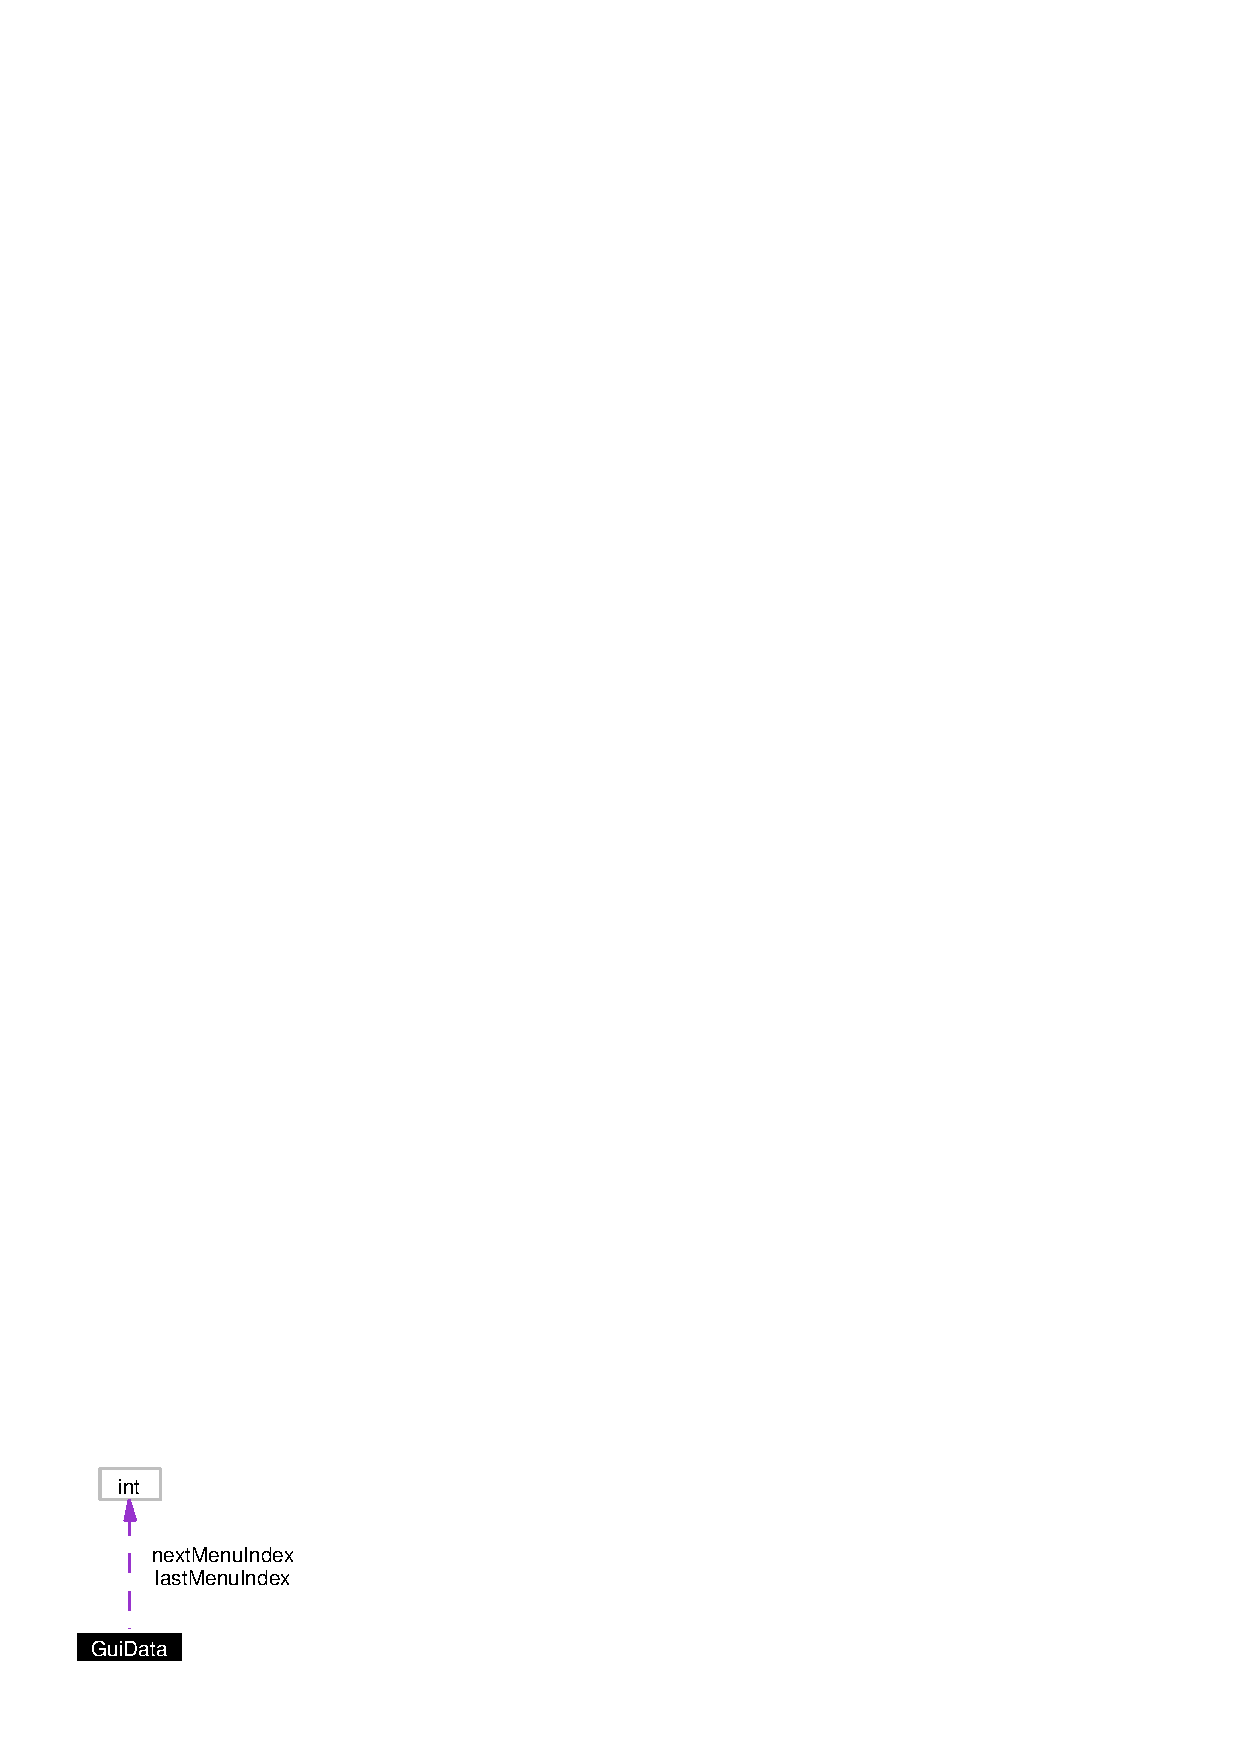
\includegraphics[width=76pt]{structGuiData__coll__graph}
\end{center}
\end{figure}
\subsection*{Public Attributes}
\begin{CompactItemize}
\item 
int {\bf next\-Menu\-Index}
\item 
int {\bf last\-Menu\-Index}
\end{CompactItemize}


\subsection{Member Data Documentation}
\index{GuiData@{Gui\-Data}!lastMenuIndex@{lastMenuIndex}}
\index{lastMenuIndex@{lastMenuIndex}!GuiData@{Gui\-Data}}
\subsubsection{\setlength{\rightskip}{0pt plus 5cm}int {\bf Gui\-Data::last\-Menu\-Index}}\label{structGuiData_o1}


\index{GuiData@{Gui\-Data}!nextMenuIndex@{nextMenuIndex}}
\index{nextMenuIndex@{nextMenuIndex}!GuiData@{Gui\-Data}}
\subsubsection{\setlength{\rightskip}{0pt plus 5cm}int {\bf Gui\-Data::next\-Menu\-Index}}\label{structGuiData_o0}




The documentation for this struct was generated from the following file:\begin{CompactItemize}
\item 
src/{\bf system.hpp}\end{CompactItemize}

\section{Gui\-Engine Class Reference}
\label{classGuiEngine}\index{GuiEngine@{GuiEngine}}
{\tt \#include $<$gui\-Engine.hpp$>$}

Collaboration diagram for Gui\-Engine:\begin{figure}[H]
\begin{center}
\leavevmode
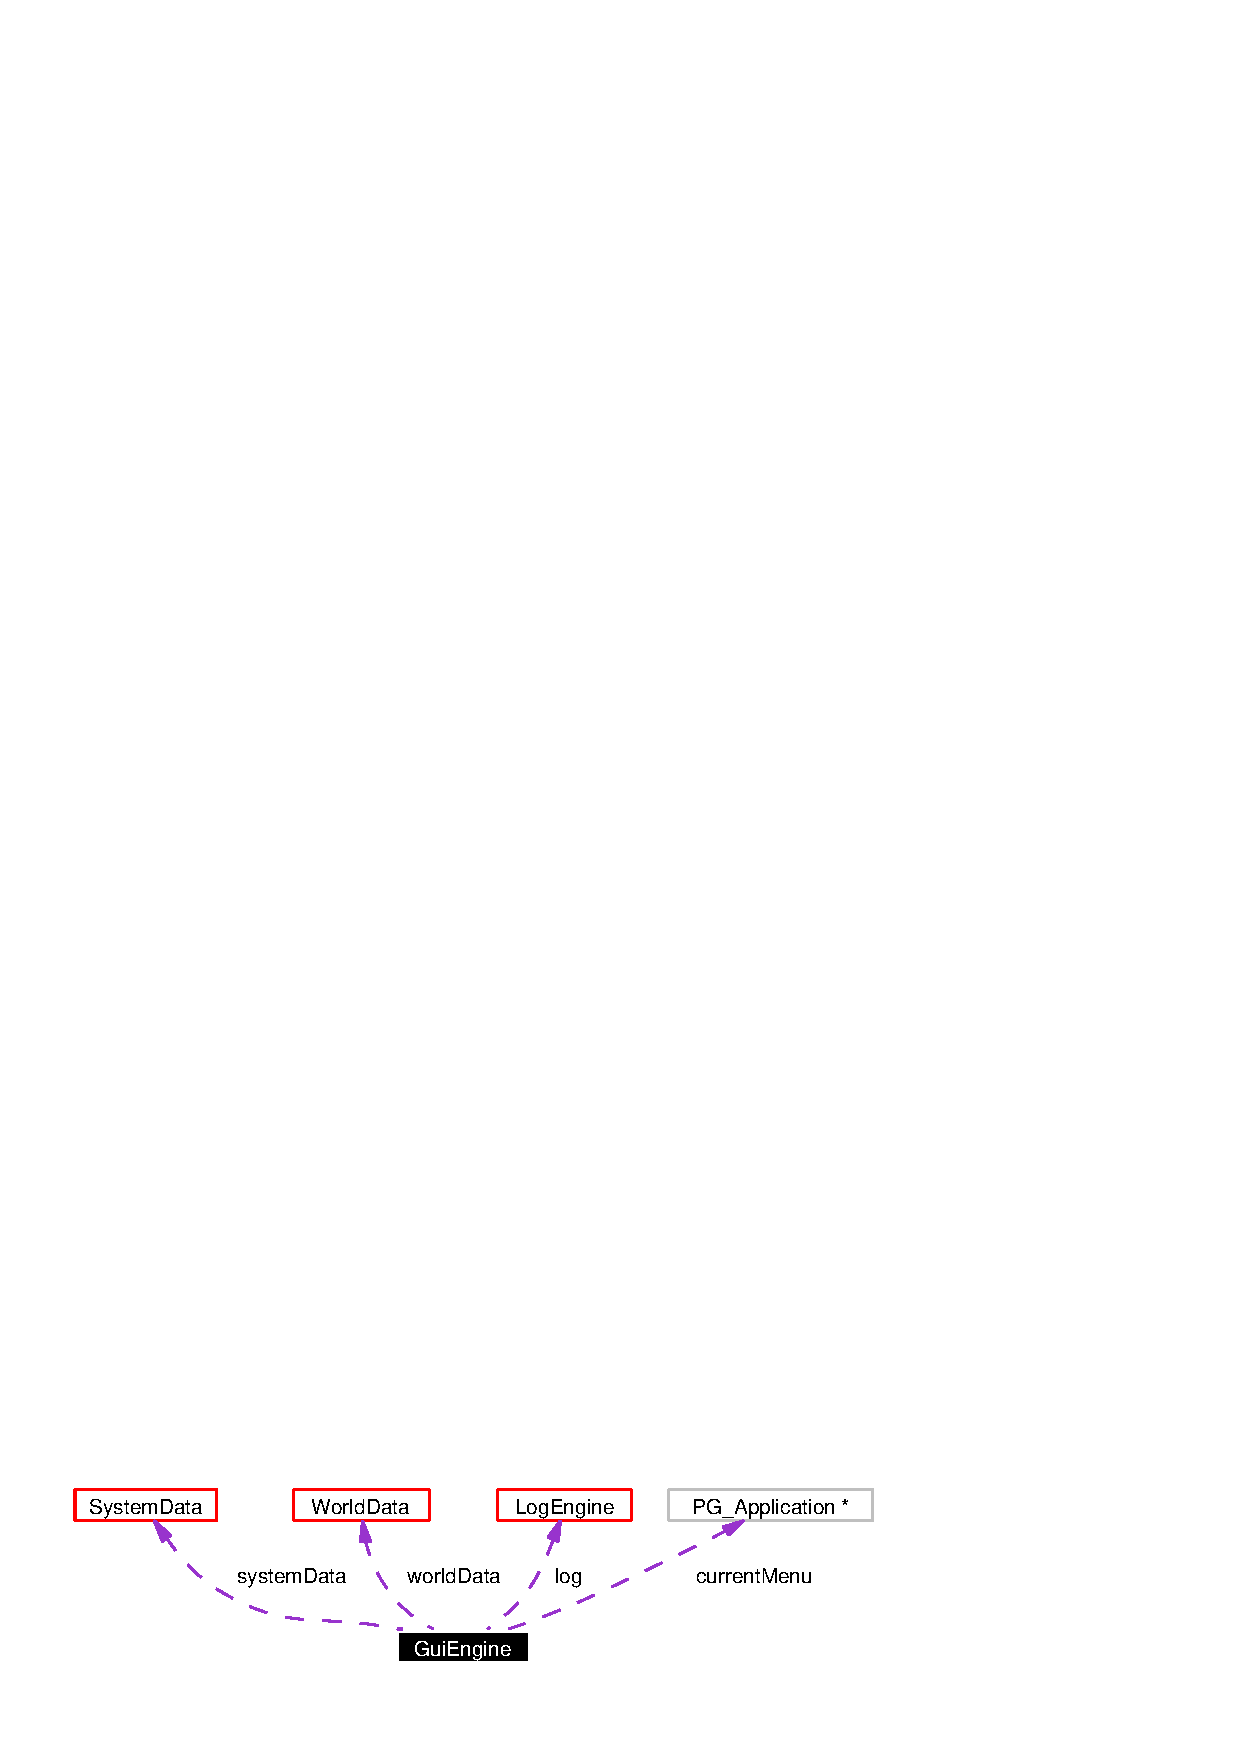
\includegraphics[width=223pt]{classGuiEngine__coll__graph}
\end{center}
\end{figure}
\subsection*{Public Member Functions}
\begin{CompactItemize}
\item 
int {\bf options\-Menu} (void)
\item 
int {\bf main\-Menu} (void)
\item 
int {\bf test\-Basic\-Paragui} (void)
\item 
int {\bf start} ({\bf World\-Data} $\ast$wrl\-Data, {\bf System\-Data} $\ast$sys\-Data)
\item 
int {\bf step} (void)
\item 
int {\bf stop} (void)
\item 
PG\_\-Application $\ast$ {\bf get\-Current\-Menu} (void)
\item 
{\bf World\-Data} $\ast$ {\bf get\-World\-Data} (void)
\item 
{\bf System\-Data} $\ast$ {\bf get\-System\-Data} (void)
\item 
{\bf Log\-Engine} $\ast$ {\bf get\-Log} (void)
\end{CompactItemize}
\subsection*{Private Attributes}
\begin{CompactItemize}
\item 
{\bf Log\-Engine} {\bf log}
\item 
{\bf World\-Data} $\ast$ {\bf world\-Data}
\item 
{\bf System\-Data} $\ast$ {\bf system\-Data}
\item 
PG\_\-Application $\ast$ {\bf current\-Menu}
\end{CompactItemize}


\subsection{Member Function Documentation}
\index{GuiEngine@{Gui\-Engine}!getCurrentMenu@{getCurrentMenu}}
\index{getCurrentMenu@{getCurrentMenu}!GuiEngine@{Gui\-Engine}}
\subsubsection{\setlength{\rightskip}{0pt plus 5cm}PG\_\-Application $\ast$ Gui\-Engine::get\-Current\-Menu (void)}\label{classGuiEngine_a6}


\index{GuiEngine@{Gui\-Engine}!getLog@{getLog}}
\index{getLog@{getLog}!GuiEngine@{Gui\-Engine}}
\subsubsection{\setlength{\rightskip}{0pt plus 5cm}{\bf Log\-Engine} $\ast$ Gui\-Engine::get\-Log (void)}\label{classGuiEngine_a9}


\index{GuiEngine@{Gui\-Engine}!getSystemData@{getSystemData}}
\index{getSystemData@{getSystemData}!GuiEngine@{Gui\-Engine}}
\subsubsection{\setlength{\rightskip}{0pt plus 5cm}{\bf System\-Data} $\ast$ Gui\-Engine::get\-System\-Data (void)}\label{classGuiEngine_a8}


\index{GuiEngine@{Gui\-Engine}!getWorldData@{getWorldData}}
\index{getWorldData@{getWorldData}!GuiEngine@{Gui\-Engine}}
\subsubsection{\setlength{\rightskip}{0pt plus 5cm}{\bf World\-Data} $\ast$ Gui\-Engine::get\-World\-Data (void)}\label{classGuiEngine_a7}


\index{GuiEngine@{Gui\-Engine}!mainMenu@{mainMenu}}
\index{mainMenu@{mainMenu}!GuiEngine@{Gui\-Engine}}
\subsubsection{\setlength{\rightskip}{0pt plus 5cm}int Gui\-Engine::main\-Menu (void)}\label{classGuiEngine_a1}


\index{GuiEngine@{Gui\-Engine}!optionsMenu@{optionsMenu}}
\index{optionsMenu@{optionsMenu}!GuiEngine@{Gui\-Engine}}
\subsubsection{\setlength{\rightskip}{0pt plus 5cm}int Gui\-Engine::options\-Menu (void)}\label{classGuiEngine_a0}


\index{GuiEngine@{Gui\-Engine}!start@{start}}
\index{start@{start}!GuiEngine@{Gui\-Engine}}
\subsubsection{\setlength{\rightskip}{0pt plus 5cm}int Gui\-Engine::start ({\bf World\-Data} $\ast$ {\em wrl\-Data}, {\bf System\-Data} $\ast$ {\em sys\-Data})}\label{classGuiEngine_a3}


\index{GuiEngine@{Gui\-Engine}!step@{step}}
\index{step@{step}!GuiEngine@{Gui\-Engine}}
\subsubsection{\setlength{\rightskip}{0pt plus 5cm}int Gui\-Engine::step (void)}\label{classGuiEngine_a4}


\index{GuiEngine@{Gui\-Engine}!stop@{stop}}
\index{stop@{stop}!GuiEngine@{Gui\-Engine}}
\subsubsection{\setlength{\rightskip}{0pt plus 5cm}int Gui\-Engine::stop (void)}\label{classGuiEngine_a5}


\index{GuiEngine@{Gui\-Engine}!testBasicParagui@{testBasicParagui}}
\index{testBasicParagui@{testBasicParagui}!GuiEngine@{Gui\-Engine}}
\subsubsection{\setlength{\rightskip}{0pt plus 5cm}int Gui\-Engine::test\-Basic\-Paragui (void)}\label{classGuiEngine_a2}




\subsection{Member Data Documentation}
\index{GuiEngine@{Gui\-Engine}!currentMenu@{currentMenu}}
\index{currentMenu@{currentMenu}!GuiEngine@{Gui\-Engine}}
\subsubsection{\setlength{\rightskip}{0pt plus 5cm}PG\_\-Application$\ast$ {\bf Gui\-Engine::current\-Menu}\hspace{0.3cm}{\tt  [private]}}\label{classGuiEngine_r3}


\index{GuiEngine@{Gui\-Engine}!log@{log}}
\index{log@{log}!GuiEngine@{Gui\-Engine}}
\subsubsection{\setlength{\rightskip}{0pt plus 5cm}{\bf Log\-Engine} {\bf Gui\-Engine::log}\hspace{0.3cm}{\tt  [private]}}\label{classGuiEngine_r0}


\index{GuiEngine@{Gui\-Engine}!systemData@{systemData}}
\index{systemData@{systemData}!GuiEngine@{Gui\-Engine}}
\subsubsection{\setlength{\rightskip}{0pt plus 5cm}{\bf System\-Data}$\ast$ {\bf Gui\-Engine::system\-Data}\hspace{0.3cm}{\tt  [private]}}\label{classGuiEngine_r2}


\index{GuiEngine@{Gui\-Engine}!worldData@{worldData}}
\index{worldData@{worldData}!GuiEngine@{Gui\-Engine}}
\subsubsection{\setlength{\rightskip}{0pt plus 5cm}{\bf World\-Data}$\ast$ {\bf Gui\-Engine::world\-Data}\hspace{0.3cm}{\tt  [private]}}\label{classGuiEngine_r1}




The documentation for this class was generated from the following files:\begin{CompactItemize}
\item 
src/gui/{\bf gui\-Engine.hpp}\item 
src/gui/{\bf gui\-Engine.cpp}\end{CompactItemize}

\section{Input\-Data Struct Reference}
\label{structInputData}\index{InputData@{InputData}}
{\tt \#include $<$system.hpp$>$}



The documentation for this struct was generated from the following file:\begin{CompactItemize}
\item 
src/{\bf system.hpp}\end{CompactItemize}

\section{Input\-Engine Class Reference}
\label{classInputEngine}\index{InputEngine@{InputEngine}}
{\tt \#include $<$input\-Engine.hpp$>$}

Collaboration diagram for Input\-Engine:\begin{figure}[H]
\begin{center}
\leavevmode
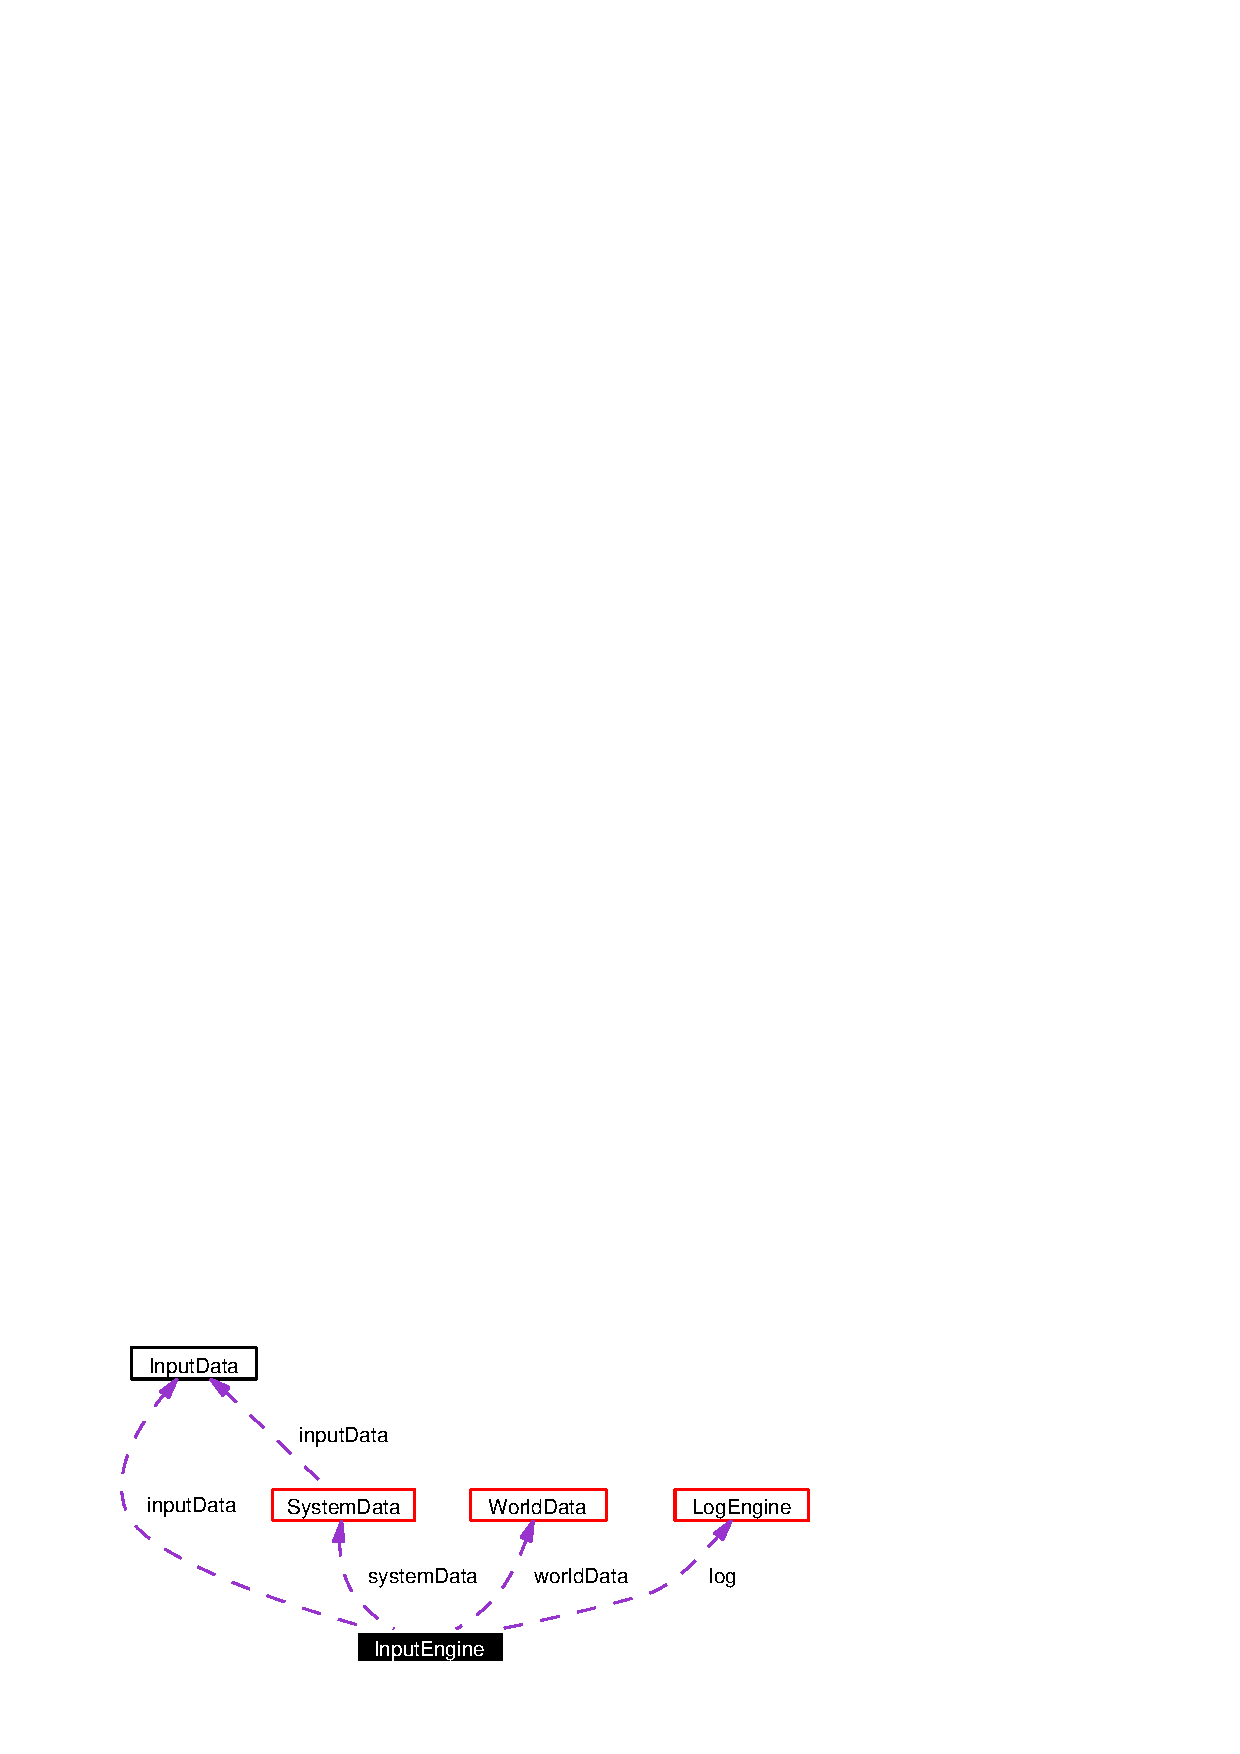
\includegraphics[width=194pt]{classInputEngine__coll__graph}
\end{center}
\end{figure}
\subsection*{Public Member Functions}
\begin{CompactItemize}
\item 
int {\bf start} ({\bf World\-Data} $\ast$wrl\-Data, {\bf System\-Data} $\ast$sys\-Data)
\item 
int {\bf step} (void)
\item 
void {\bf process\-Input} (SDLKey key\-Symbol)
\item 
int {\bf stop} (void)
\end{CompactItemize}
\subsection*{Private Attributes}
\begin{CompactItemize}
\item 
{\bf Log\-Engine} {\bf log}
\item 
{\bf Input\-Data} $\ast$ {\bf input\-Data}
\item 
{\bf System\-Data} $\ast$ {\bf system\-Data}
\item 
{\bf World\-Data} $\ast$ {\bf world\-Data}
\end{CompactItemize}


\subsection{Member Function Documentation}
\index{InputEngine@{Input\-Engine}!processInput@{processInput}}
\index{processInput@{processInput}!InputEngine@{Input\-Engine}}
\subsubsection{\setlength{\rightskip}{0pt plus 5cm}void Input\-Engine::process\-Input (SDLKey {\em key\-Symbol})}\label{classInputEngine_a2}


\index{InputEngine@{Input\-Engine}!start@{start}}
\index{start@{start}!InputEngine@{Input\-Engine}}
\subsubsection{\setlength{\rightskip}{0pt plus 5cm}int Input\-Engine::start ({\bf World\-Data} $\ast$ {\em wrl\-Data}, {\bf System\-Data} $\ast$ {\em sys\-Data})}\label{classInputEngine_a0}


\index{InputEngine@{Input\-Engine}!step@{step}}
\index{step@{step}!InputEngine@{Input\-Engine}}
\subsubsection{\setlength{\rightskip}{0pt plus 5cm}int Input\-Engine::step (void)}\label{classInputEngine_a1}


\index{InputEngine@{Input\-Engine}!stop@{stop}}
\index{stop@{stop}!InputEngine@{Input\-Engine}}
\subsubsection{\setlength{\rightskip}{0pt plus 5cm}int Input\-Engine::stop (void)}\label{classInputEngine_a3}




\subsection{Member Data Documentation}
\index{InputEngine@{Input\-Engine}!inputData@{inputData}}
\index{inputData@{inputData}!InputEngine@{Input\-Engine}}
\subsubsection{\setlength{\rightskip}{0pt plus 5cm}{\bf Input\-Data}$\ast$ {\bf Input\-Engine::input\-Data}\hspace{0.3cm}{\tt  [private]}}\label{classInputEngine_r1}


\index{InputEngine@{Input\-Engine}!log@{log}}
\index{log@{log}!InputEngine@{Input\-Engine}}
\subsubsection{\setlength{\rightskip}{0pt plus 5cm}{\bf Log\-Engine} {\bf Input\-Engine::log}\hspace{0.3cm}{\tt  [private]}}\label{classInputEngine_r0}


\index{InputEngine@{Input\-Engine}!systemData@{systemData}}
\index{systemData@{systemData}!InputEngine@{Input\-Engine}}
\subsubsection{\setlength{\rightskip}{0pt plus 5cm}{\bf System\-Data}$\ast$ {\bf Input\-Engine::system\-Data}\hspace{0.3cm}{\tt  [private]}}\label{classInputEngine_r2}


\index{InputEngine@{Input\-Engine}!worldData@{worldData}}
\index{worldData@{worldData}!InputEngine@{Input\-Engine}}
\subsubsection{\setlength{\rightskip}{0pt plus 5cm}{\bf World\-Data}$\ast$ {\bf Input\-Engine::world\-Data}\hspace{0.3cm}{\tt  [private]}}\label{classInputEngine_r3}




The documentation for this class was generated from the following files:\begin{CompactItemize}
\item 
src/input/{\bf input\-Engine.hpp}\item 
src/input/{\bf input\-Engine.cpp}\end{CompactItemize}

\section{Key\-Listener Class Reference}
\label{classKeyListener}\index{KeyListener@{KeyListener}}
Inheritance diagram for Key\-Listener::\begin{figure}[H]
\begin{center}
\leavevmode
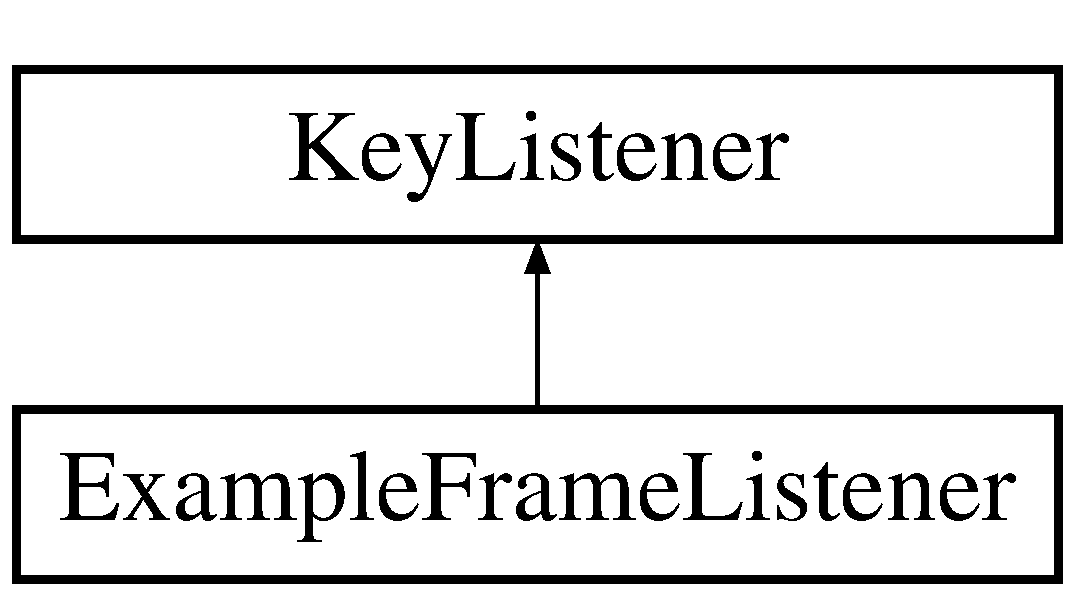
\includegraphics[height=2cm]{classKeyListener}
\end{center}
\end{figure}


The documentation for this class was generated from the following file:\begin{CompactItemize}
\item 
src/graphics/{\bf Example\-Frame\-Listener.h}\end{CompactItemize}

\section{Log\-Engine Class Reference}
\label{classLogEngine}\index{LogEngine@{LogEngine}}
{\tt \#include $<$log\-Engine.hpp$>$}

Collaboration diagram for Log\-Engine:\begin{figure}[H]
\begin{center}
\leavevmode
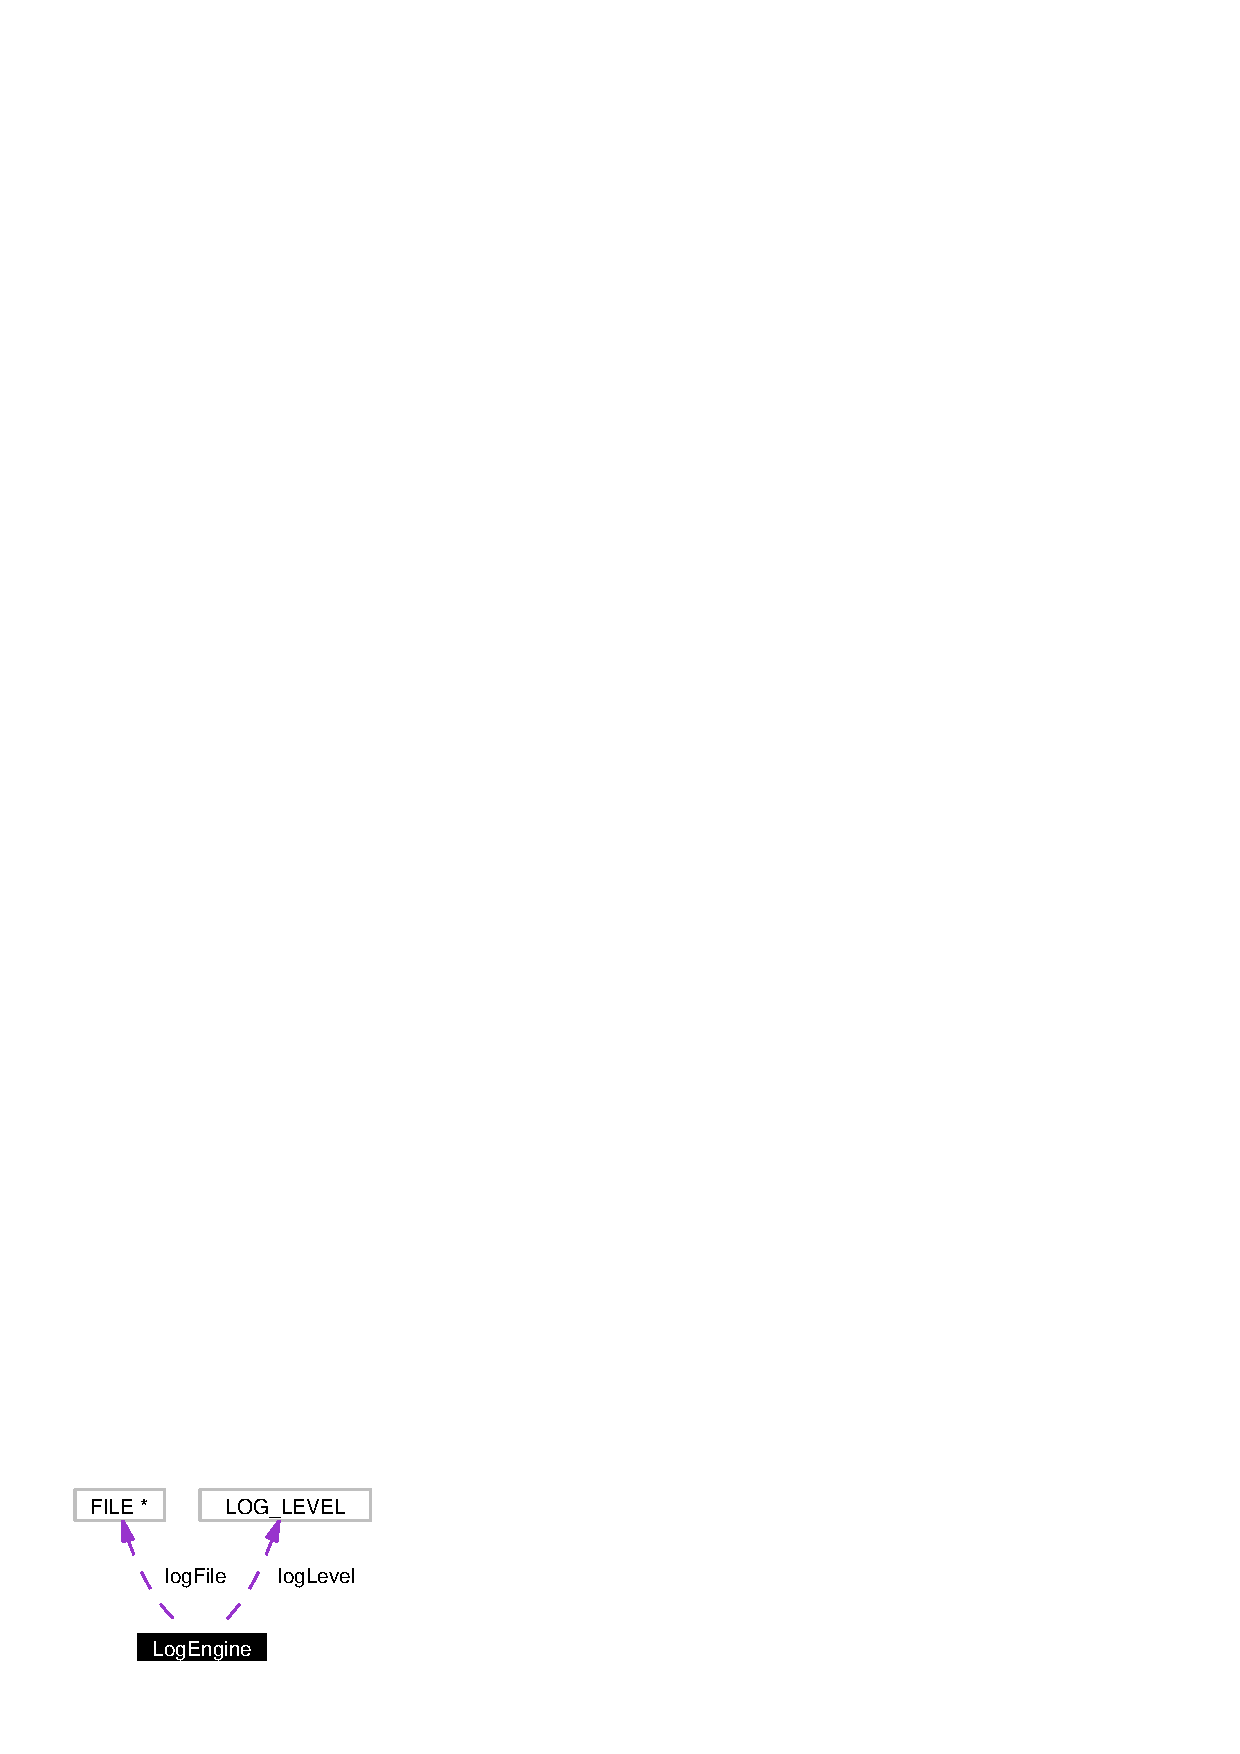
\includegraphics[width=95pt]{classLogEngine__coll__graph}
\end{center}
\end{figure}
\subsection*{Public Member Functions}
\begin{CompactItemize}
\item 
int {\bf start} ({\bf LOG\_\-LEVEL} level, const char $\ast$file\-Path, bool append\-Mode=false)
\item 
int {\bf put} ({\bf LOG\_\-LEVEL} level, const char $\ast$text\-To\-Log, bool use\-New\-Line=true)
\item 
int {\bf format} ({\bf LOG\_\-LEVEL} level, const char $\ast$text\-To\-Log\-Format,...)
\item 
int {\bf append} ({\bf LOG\_\-LEVEL} level, const char $\ast$text\-To\-Log)
\item 
int {\bf stop} (void)
\end{CompactItemize}
\subsection*{Private Attributes}
\begin{CompactItemize}
\item 
FILE $\ast$ {\bf log\-File}
\item 
{\bf LOG\_\-LEVEL} {\bf log\-Level}
\end{CompactItemize}


\subsection{Member Function Documentation}
\index{LogEngine@{Log\-Engine}!append@{append}}
\index{append@{append}!LogEngine@{Log\-Engine}}
\subsubsection{\setlength{\rightskip}{0pt plus 5cm}int Log\-Engine::append ({\bf LOG\_\-LEVEL} {\em level}, const char $\ast$ {\em text\-To\-Log})}\label{classLogEngine_a3}


\index{LogEngine@{Log\-Engine}!format@{format}}
\index{format@{format}!LogEngine@{Log\-Engine}}
\subsubsection{\setlength{\rightskip}{0pt plus 5cm}int Log\-Engine::format ({\bf LOG\_\-LEVEL} {\em level}, const char $\ast$ {\em text\-To\-Log\-Format}, ...)}\label{classLogEngine_a2}


\index{LogEngine@{Log\-Engine}!put@{put}}
\index{put@{put}!LogEngine@{Log\-Engine}}
\subsubsection{\setlength{\rightskip}{0pt plus 5cm}int Log\-Engine::put ({\bf LOG\_\-LEVEL} {\em level}, const char $\ast$ {\em text\-To\-Log}, bool {\em use\-New\-Line} = true)}\label{classLogEngine_a1}


\index{LogEngine@{Log\-Engine}!start@{start}}
\index{start@{start}!LogEngine@{Log\-Engine}}
\subsubsection{\setlength{\rightskip}{0pt plus 5cm}int Log\-Engine::start ({\bf LOG\_\-LEVEL} {\em level}, const char $\ast$ {\em file\-Path}, bool {\em append\-Mode} = false)}\label{classLogEngine_a0}


\index{LogEngine@{Log\-Engine}!stop@{stop}}
\index{stop@{stop}!LogEngine@{Log\-Engine}}
\subsubsection{\setlength{\rightskip}{0pt plus 5cm}int Log\-Engine::stop (void)}\label{classLogEngine_a4}




\subsection{Member Data Documentation}
\index{LogEngine@{Log\-Engine}!logFile@{logFile}}
\index{logFile@{logFile}!LogEngine@{Log\-Engine}}
\subsubsection{\setlength{\rightskip}{0pt plus 5cm}FILE$\ast$ {\bf Log\-Engine::log\-File}\hspace{0.3cm}{\tt  [private]}}\label{classLogEngine_r0}


\index{LogEngine@{Log\-Engine}!logLevel@{logLevel}}
\index{logLevel@{logLevel}!LogEngine@{Log\-Engine}}
\subsubsection{\setlength{\rightskip}{0pt plus 5cm}{\bf LOG\_\-LEVEL} {\bf Log\-Engine::log\-Level}\hspace{0.3cm}{\tt  [private]}}\label{classLogEngine_r1}




The documentation for this class was generated from the following files:\begin{CompactItemize}
\item 
src/log/{\bf log\-Engine.hpp}\item 
src/log/{\bf log\-Engine.cpp}\end{CompactItemize}

\section{PG\_\-Event\-Object Class Reference}
\label{classPG__EventObject}\index{PG_EventObject@{PG\_\-EventObject}}
Inheritance diagram for PG\_\-Event\-Object::\begin{figure}[H]
\begin{center}
\leavevmode
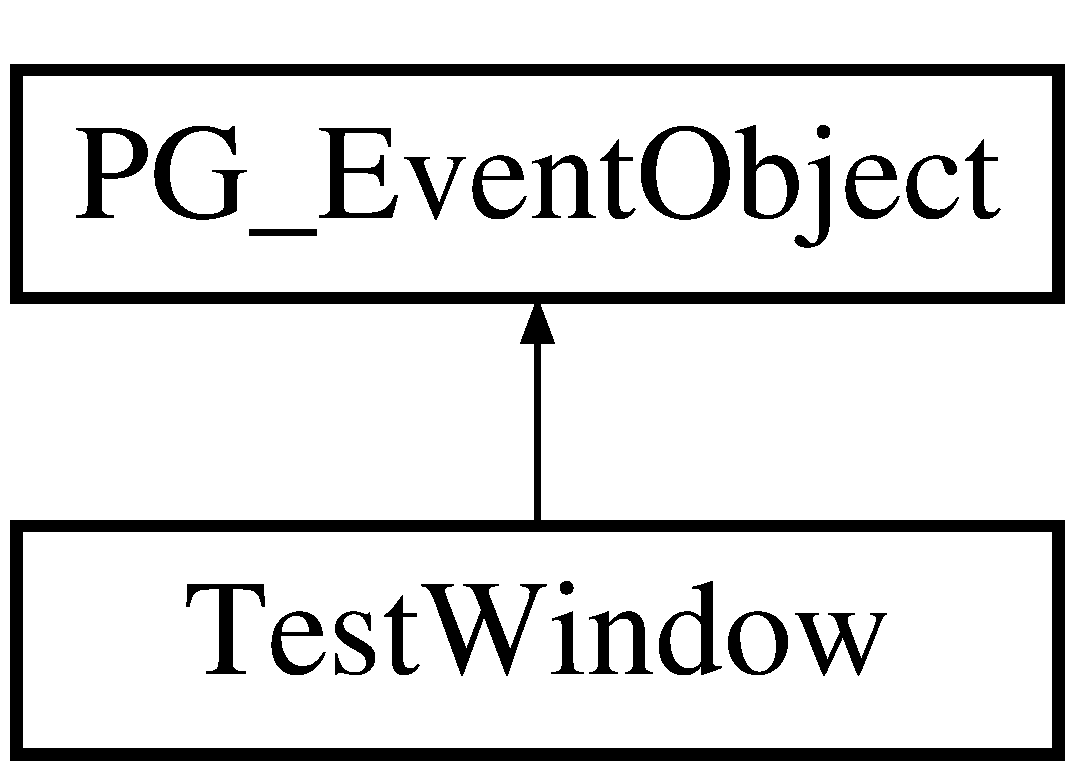
\includegraphics[height=2cm]{classPG__EventObject}
\end{center}
\end{figure}


The documentation for this class was generated from the following file:\begin{CompactItemize}
\item 
src/gui/{\bf test\_\-paragui.cpp}\end{CompactItemize}

\section{PG\_\-Window Class Reference}
\label{classPG__Window}\index{PG_Window@{PG\_\-Window}}
Inheritance diagram for PG\_\-Window::\begin{figure}[H]
\begin{center}
\leavevmode
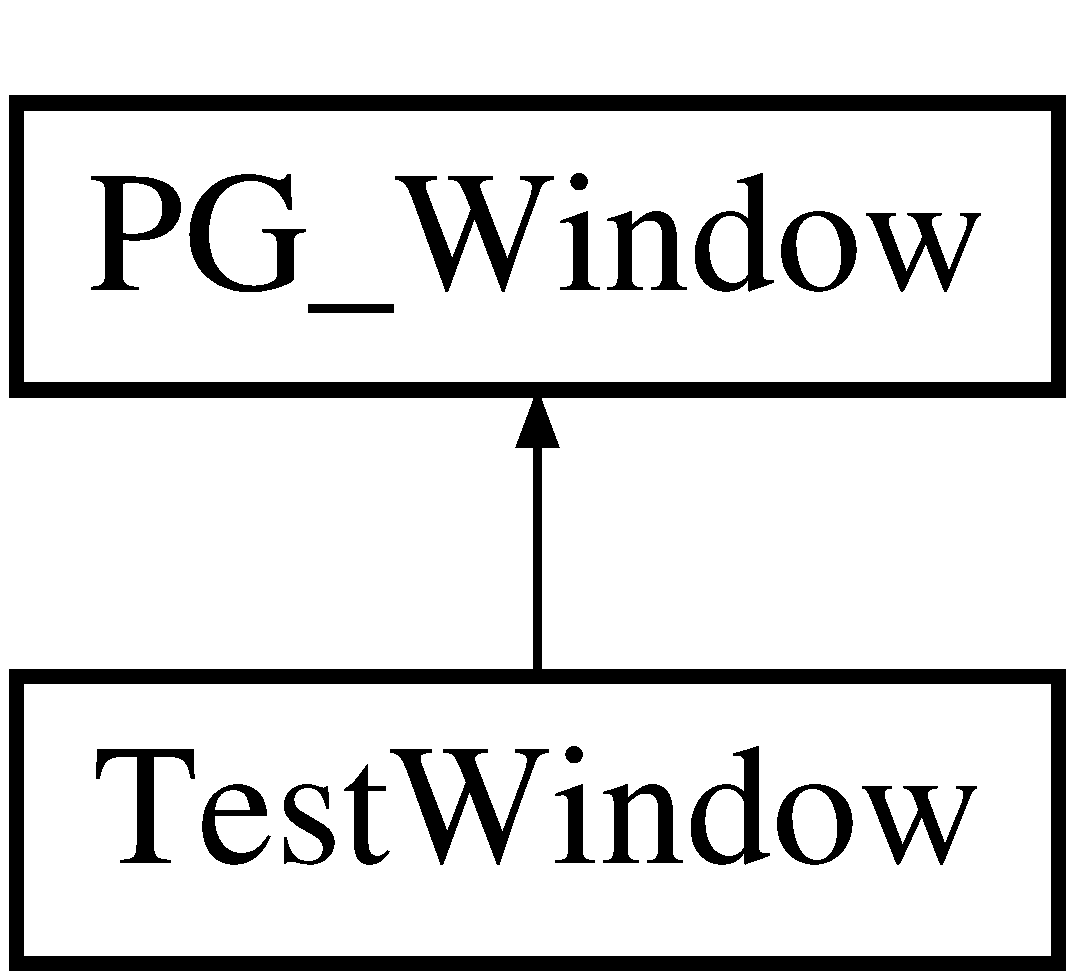
\includegraphics[height=2cm]{classPG__Window}
\end{center}
\end{figure}


The documentation for this class was generated from the following file:\begin{CompactItemize}
\item 
src/gui/{\bf test\_\-paragui.cpp}\end{CompactItemize}

\section{Physics\-Data Struct Reference}
\label{structPhysicsData}\index{PhysicsData@{PhysicsData}}
{\tt \#include $<$system.hpp$>$}

Collaboration diagram for Physics\-Data:\begin{figure}[H]
\begin{center}
\leavevmode
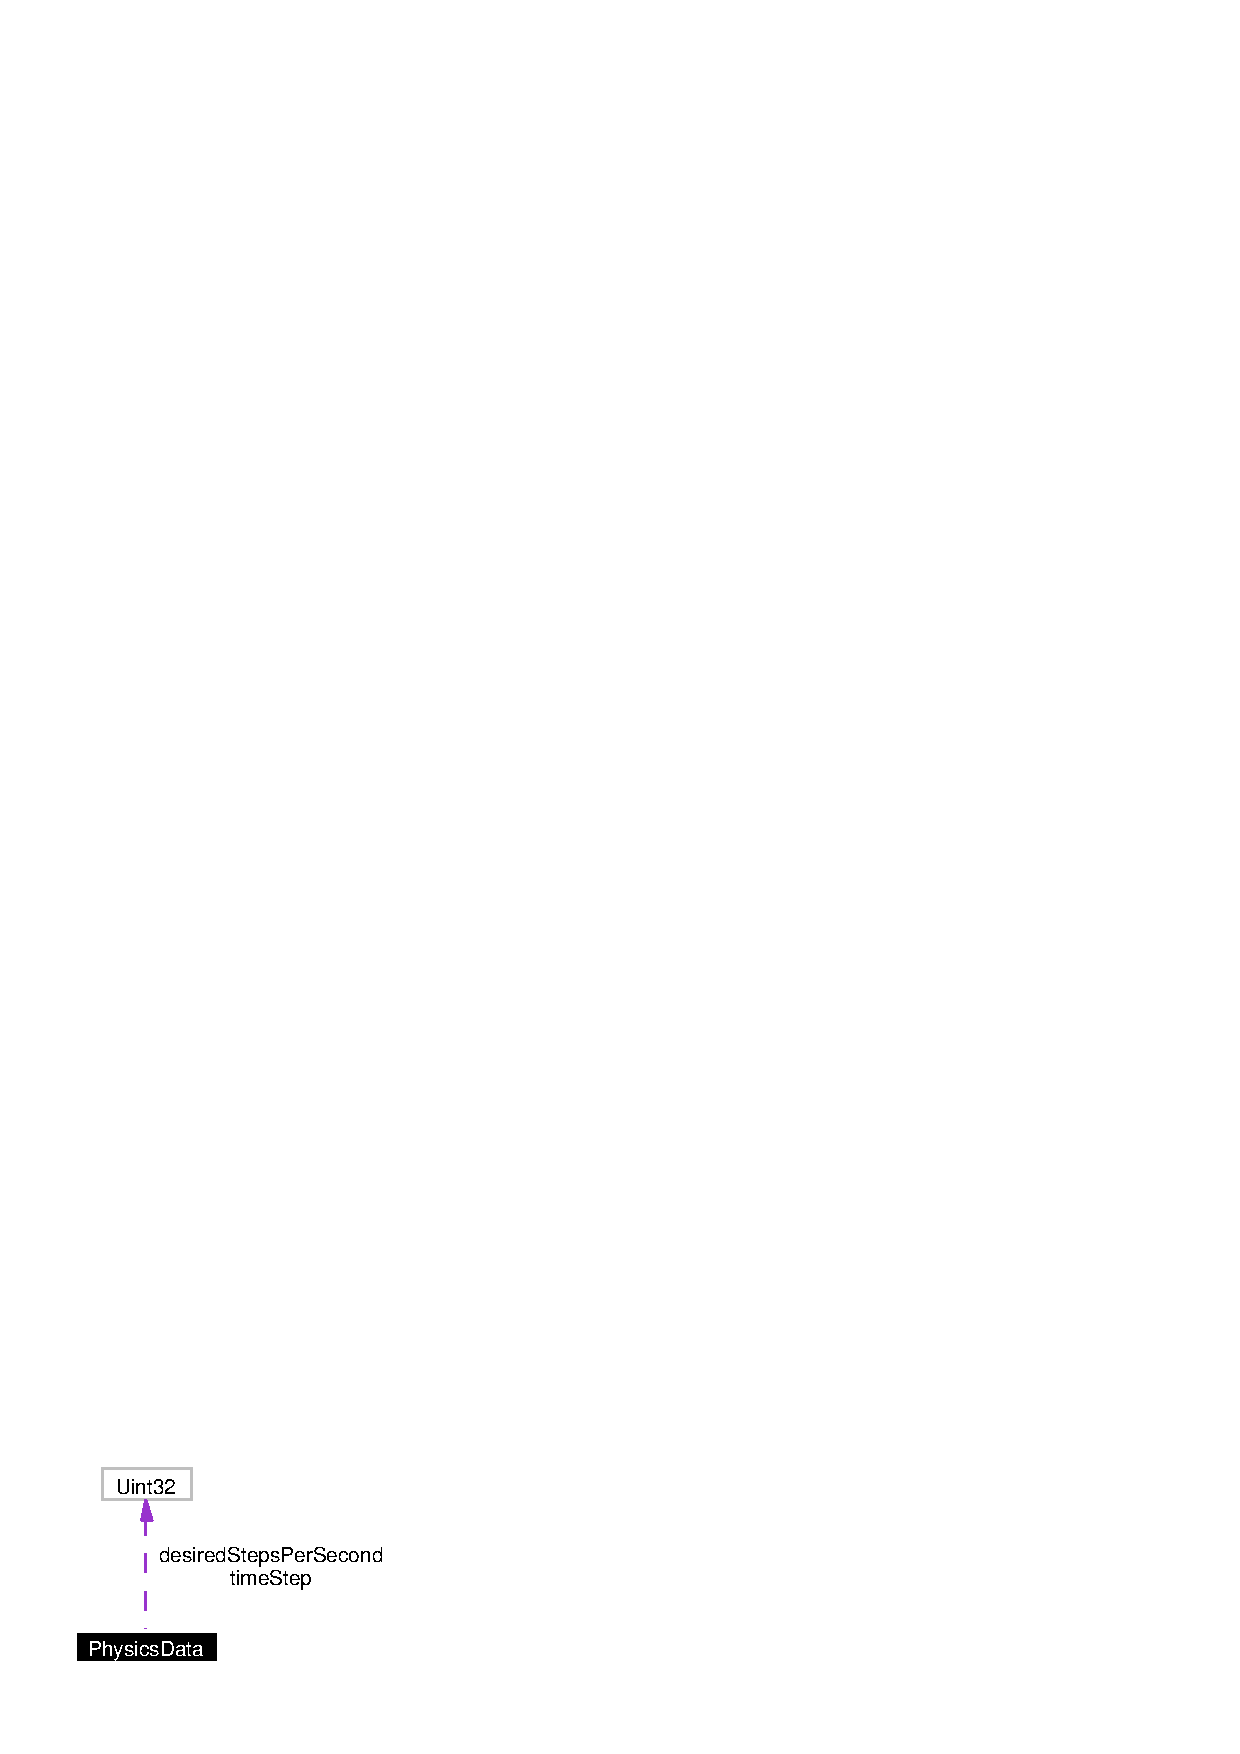
\includegraphics[width=95pt]{structPhysicsData__coll__graph}
\end{center}
\end{figure}
\subsection*{Public Attributes}
\begin{CompactItemize}
\item 
Uint32 {\bf time\-Step}
\item 
Uint32 {\bf desired\-Steps\-Per\-Second}
\end{CompactItemize}


\subsection{Member Data Documentation}
\index{PhysicsData@{Physics\-Data}!desiredStepsPerSecond@{desiredStepsPerSecond}}
\index{desiredStepsPerSecond@{desiredStepsPerSecond}!PhysicsData@{Physics\-Data}}
\subsubsection{\setlength{\rightskip}{0pt plus 5cm}Uint32 {\bf Physics\-Data::desired\-Steps\-Per\-Second}}\label{structPhysicsData_o1}


\index{PhysicsData@{Physics\-Data}!timeStep@{timeStep}}
\index{timeStep@{timeStep}!PhysicsData@{Physics\-Data}}
\subsubsection{\setlength{\rightskip}{0pt plus 5cm}Uint32 {\bf Physics\-Data::time\-Step}}\label{structPhysicsData_o0}




The documentation for this struct was generated from the following file:\begin{CompactItemize}
\item 
src/{\bf system.hpp}\end{CompactItemize}

\section{Physics\-Engine Class Reference}
\label{classPhysicsEngine}\index{PhysicsEngine@{PhysicsEngine}}
{\tt \#include $<$physics\-Engine.hpp$>$}

Collaboration diagram for Physics\-Engine:\begin{figure}[H]
\begin{center}
\leavevmode
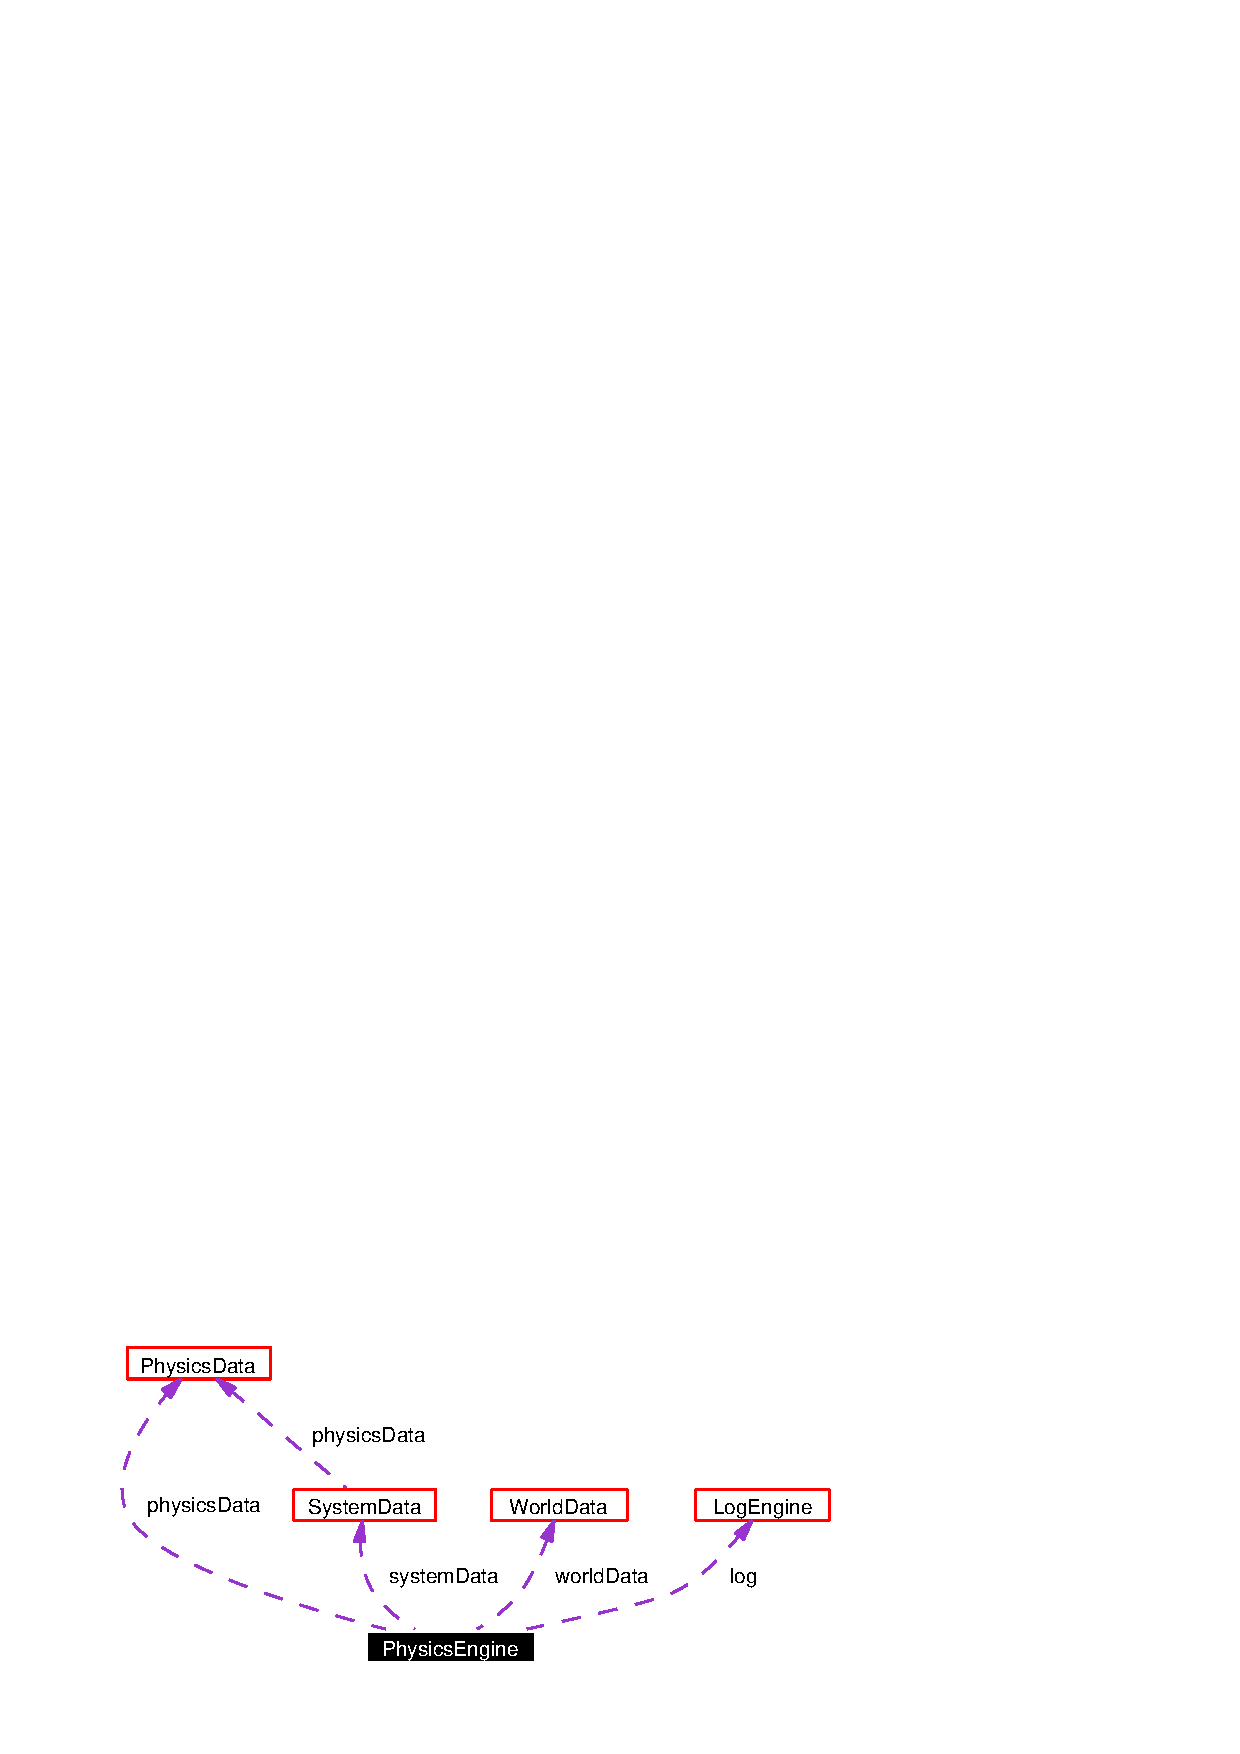
\includegraphics[width=199pt]{classPhysicsEngine__coll__graph}
\end{center}
\end{figure}
\subsection*{Public Member Functions}
\begin{CompactItemize}
\item 
int {\bf start} ({\bf World\-Data} $\ast$wrl\-Data, {\bf System\-Data} $\ast$sys\-Data)
\item 
int {\bf step} (void)
\item 
int {\bf stop} (void)
\end{CompactItemize}
\subsection*{Private Attributes}
\begin{CompactItemize}
\item 
{\bf Log\-Engine} {\bf log}
\item 
{\bf Physics\-Data} $\ast$ {\bf physics\-Data}
\item 
{\bf World\-Data} $\ast$ {\bf world\-Data}
\item 
{\bf System\-Data} $\ast$ {\bf system\-Data}
\end{CompactItemize}


\subsection{Member Function Documentation}
\index{PhysicsEngine@{Physics\-Engine}!start@{start}}
\index{start@{start}!PhysicsEngine@{Physics\-Engine}}
\subsubsection{\setlength{\rightskip}{0pt plus 5cm}int Physics\-Engine::start ({\bf World\-Data} $\ast$ {\em wrl\-Data}, {\bf System\-Data} $\ast$ {\em sys\-Data})}\label{classPhysicsEngine_a0}


\index{PhysicsEngine@{Physics\-Engine}!step@{step}}
\index{step@{step}!PhysicsEngine@{Physics\-Engine}}
\subsubsection{\setlength{\rightskip}{0pt plus 5cm}int Physics\-Engine::step (void)}\label{classPhysicsEngine_a1}


\index{PhysicsEngine@{Physics\-Engine}!stop@{stop}}
\index{stop@{stop}!PhysicsEngine@{Physics\-Engine}}
\subsubsection{\setlength{\rightskip}{0pt plus 5cm}int Physics\-Engine::stop (void)}\label{classPhysicsEngine_a2}




\subsection{Member Data Documentation}
\index{PhysicsEngine@{Physics\-Engine}!log@{log}}
\index{log@{log}!PhysicsEngine@{Physics\-Engine}}
\subsubsection{\setlength{\rightskip}{0pt plus 5cm}{\bf Log\-Engine} {\bf Physics\-Engine::log}\hspace{0.3cm}{\tt  [private]}}\label{classPhysicsEngine_r0}


\index{PhysicsEngine@{Physics\-Engine}!physicsData@{physicsData}}
\index{physicsData@{physicsData}!PhysicsEngine@{Physics\-Engine}}
\subsubsection{\setlength{\rightskip}{0pt plus 5cm}{\bf Physics\-Data}$\ast$ {\bf Physics\-Engine::physics\-Data}\hspace{0.3cm}{\tt  [private]}}\label{classPhysicsEngine_r1}


\index{PhysicsEngine@{Physics\-Engine}!systemData@{systemData}}
\index{systemData@{systemData}!PhysicsEngine@{Physics\-Engine}}
\subsubsection{\setlength{\rightskip}{0pt plus 5cm}{\bf System\-Data}$\ast$ {\bf Physics\-Engine::system\-Data}\hspace{0.3cm}{\tt  [private]}}\label{classPhysicsEngine_r3}


\index{PhysicsEngine@{Physics\-Engine}!worldData@{worldData}}
\index{worldData@{worldData}!PhysicsEngine@{Physics\-Engine}}
\subsubsection{\setlength{\rightskip}{0pt plus 5cm}{\bf World\-Data}$\ast$ {\bf Physics\-Engine::world\-Data}\hspace{0.3cm}{\tt  [private]}}\label{classPhysicsEngine_r2}




The documentation for this class was generated from the following files:\begin{CompactItemize}
\item 
src/physics/{\bf physics\-Engine.hpp}\item 
src/physics/{\bf physics\-Engine.cpp}\end{CompactItemize}

\section{Rectangle Class Reference}
\label{classRectangle}\index{Rectangle@{Rectangle}}
{\tt \#include $<$world.hpp$>$}

Collaboration diagram for Rectangle:\begin{figure}[H]
\begin{center}
\leavevmode
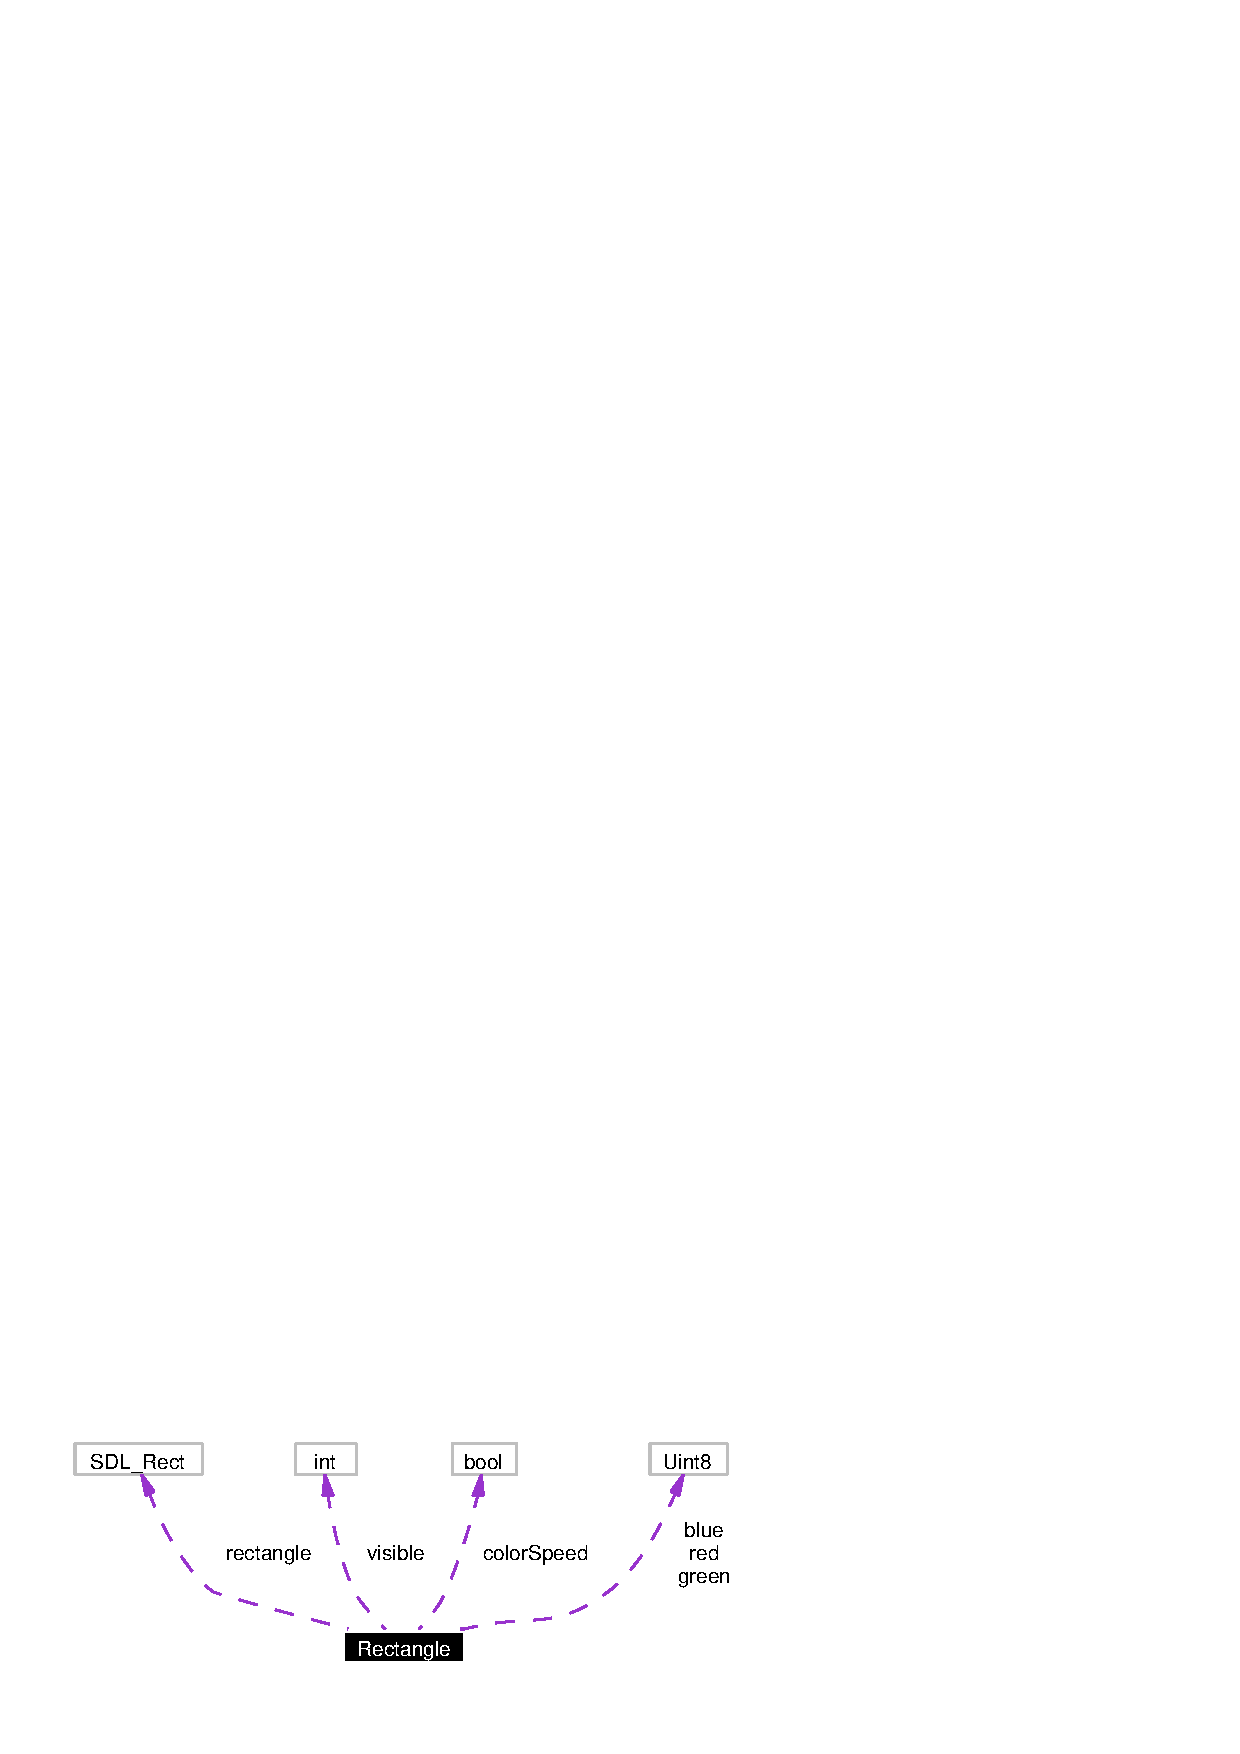
\includegraphics[width=184pt]{classRectangle__coll__graph}
\end{center}
\end{figure}
\subsection*{Public Member Functions}
\begin{CompactItemize}
\item 
void {\bf set\-Position} (Sint16 new\-Pos\-X, Sint16 new\-Pos\-Y)
\item 
Sint16 {\bf get\-Position\-X} (void)
\item 
Sint16 {\bf get\-Position\-Y} (void)
\item 
void {\bf set\-Size} (Uint16 new\-Width, Uint16 new\-Height)
\item 
Sint16 {\bf get\-Size\-X} (void)
\item 
Sint16 {\bf get\-Size\-Y} (void)
\item 
void {\bf set\-Visible} (int visibility)
\item 
int {\bf is\-Visible} ()
\item 
SDL\_\-Rect $\ast$ {\bf sdl\-Rectangle} ()
\end{CompactItemize}
\subsection*{Public Attributes}
\begin{CompactItemize}
\item 
Uint8 {\bf red}
\item 
Uint8 {\bf green}
\item 
Uint8 {\bf blue}
\item 
bool {\bf color\-Speed}
\end{CompactItemize}
\subsection*{Private Attributes}
\begin{CompactItemize}
\item 
SDL\_\-Rect {\bf rectangle}
\item 
int {\bf visible}
\end{CompactItemize}


\subsection{Member Function Documentation}
\index{Rectangle@{Rectangle}!getPositionX@{getPositionX}}
\index{getPositionX@{getPositionX}!Rectangle@{Rectangle}}
\subsubsection{\setlength{\rightskip}{0pt plus 5cm}Sint16 Rectangle::get\-Position\-X (void)}\label{classRectangle_a1}


\index{Rectangle@{Rectangle}!getPositionY@{getPositionY}}
\index{getPositionY@{getPositionY}!Rectangle@{Rectangle}}
\subsubsection{\setlength{\rightskip}{0pt plus 5cm}Sint16 Rectangle::get\-Position\-Y (void)}\label{classRectangle_a2}


\index{Rectangle@{Rectangle}!getSizeX@{getSizeX}}
\index{getSizeX@{getSizeX}!Rectangle@{Rectangle}}
\subsubsection{\setlength{\rightskip}{0pt plus 5cm}Sint16 Rectangle::get\-Size\-X (void)}\label{classRectangle_a4}


\index{Rectangle@{Rectangle}!getSizeY@{getSizeY}}
\index{getSizeY@{getSizeY}!Rectangle@{Rectangle}}
\subsubsection{\setlength{\rightskip}{0pt plus 5cm}Sint16 Rectangle::get\-Size\-Y (void)}\label{classRectangle_a5}


\index{Rectangle@{Rectangle}!isVisible@{isVisible}}
\index{isVisible@{isVisible}!Rectangle@{Rectangle}}
\subsubsection{\setlength{\rightskip}{0pt plus 5cm}int Rectangle::is\-Visible ()}\label{classRectangle_a7}


\index{Rectangle@{Rectangle}!sdlRectangle@{sdlRectangle}}
\index{sdlRectangle@{sdlRectangle}!Rectangle@{Rectangle}}
\subsubsection{\setlength{\rightskip}{0pt plus 5cm}SDL\_\-Rect $\ast$ Rectangle::sdl\-Rectangle ()}\label{classRectangle_a8}


\index{Rectangle@{Rectangle}!setPosition@{setPosition}}
\index{setPosition@{setPosition}!Rectangle@{Rectangle}}
\subsubsection{\setlength{\rightskip}{0pt plus 5cm}void Rectangle::set\-Position (Sint16 {\em new\-Pos\-X}, Sint16 {\em new\-Pos\-Y})}\label{classRectangle_a0}


\index{Rectangle@{Rectangle}!setSize@{setSize}}
\index{setSize@{setSize}!Rectangle@{Rectangle}}
\subsubsection{\setlength{\rightskip}{0pt plus 5cm}void Rectangle::set\-Size (Uint16 {\em new\-Width}, Uint16 {\em new\-Height})}\label{classRectangle_a3}


\index{Rectangle@{Rectangle}!setVisible@{setVisible}}
\index{setVisible@{setVisible}!Rectangle@{Rectangle}}
\subsubsection{\setlength{\rightskip}{0pt plus 5cm}void Rectangle::set\-Visible (int {\em visibility})}\label{classRectangle_a6}




\subsection{Member Data Documentation}
\index{Rectangle@{Rectangle}!blue@{blue}}
\index{blue@{blue}!Rectangle@{Rectangle}}
\subsubsection{\setlength{\rightskip}{0pt plus 5cm}Uint8 {\bf Rectangle::blue}}\label{classRectangle_o2}


\index{Rectangle@{Rectangle}!colorSpeed@{colorSpeed}}
\index{colorSpeed@{colorSpeed}!Rectangle@{Rectangle}}
\subsubsection{\setlength{\rightskip}{0pt plus 5cm}bool {\bf Rectangle::color\-Speed}}\label{classRectangle_o3}


\index{Rectangle@{Rectangle}!green@{green}}
\index{green@{green}!Rectangle@{Rectangle}}
\subsubsection{\setlength{\rightskip}{0pt plus 5cm}Uint8 {\bf Rectangle::green}}\label{classRectangle_o1}


\index{Rectangle@{Rectangle}!rectangle@{rectangle}}
\index{rectangle@{rectangle}!Rectangle@{Rectangle}}
\subsubsection{\setlength{\rightskip}{0pt plus 5cm}SDL\_\-Rect {\bf Rectangle::rectangle}\hspace{0.3cm}{\tt  [private]}}\label{classRectangle_r0}


\index{Rectangle@{Rectangle}!red@{red}}
\index{red@{red}!Rectangle@{Rectangle}}
\subsubsection{\setlength{\rightskip}{0pt plus 5cm}Uint8 {\bf Rectangle::red}}\label{classRectangle_o0}


\index{Rectangle@{Rectangle}!visible@{visible}}
\index{visible@{visible}!Rectangle@{Rectangle}}
\subsubsection{\setlength{\rightskip}{0pt plus 5cm}int {\bf Rectangle::visible}\hspace{0.3cm}{\tt  [private]}}\label{classRectangle_r1}




The documentation for this class was generated from the following files:\begin{CompactItemize}
\item 
src/{\bf world.hpp}\item 
src/{\bf world.cpp}\end{CompactItemize}

\section{System\-Data Class Reference}
\label{classSystemData}\index{SystemData@{SystemData}}
{\tt \#include $<$system.hpp$>$}

Collaboration diagram for System\-Data:\begin{figure}[H]
\begin{center}
\leavevmode
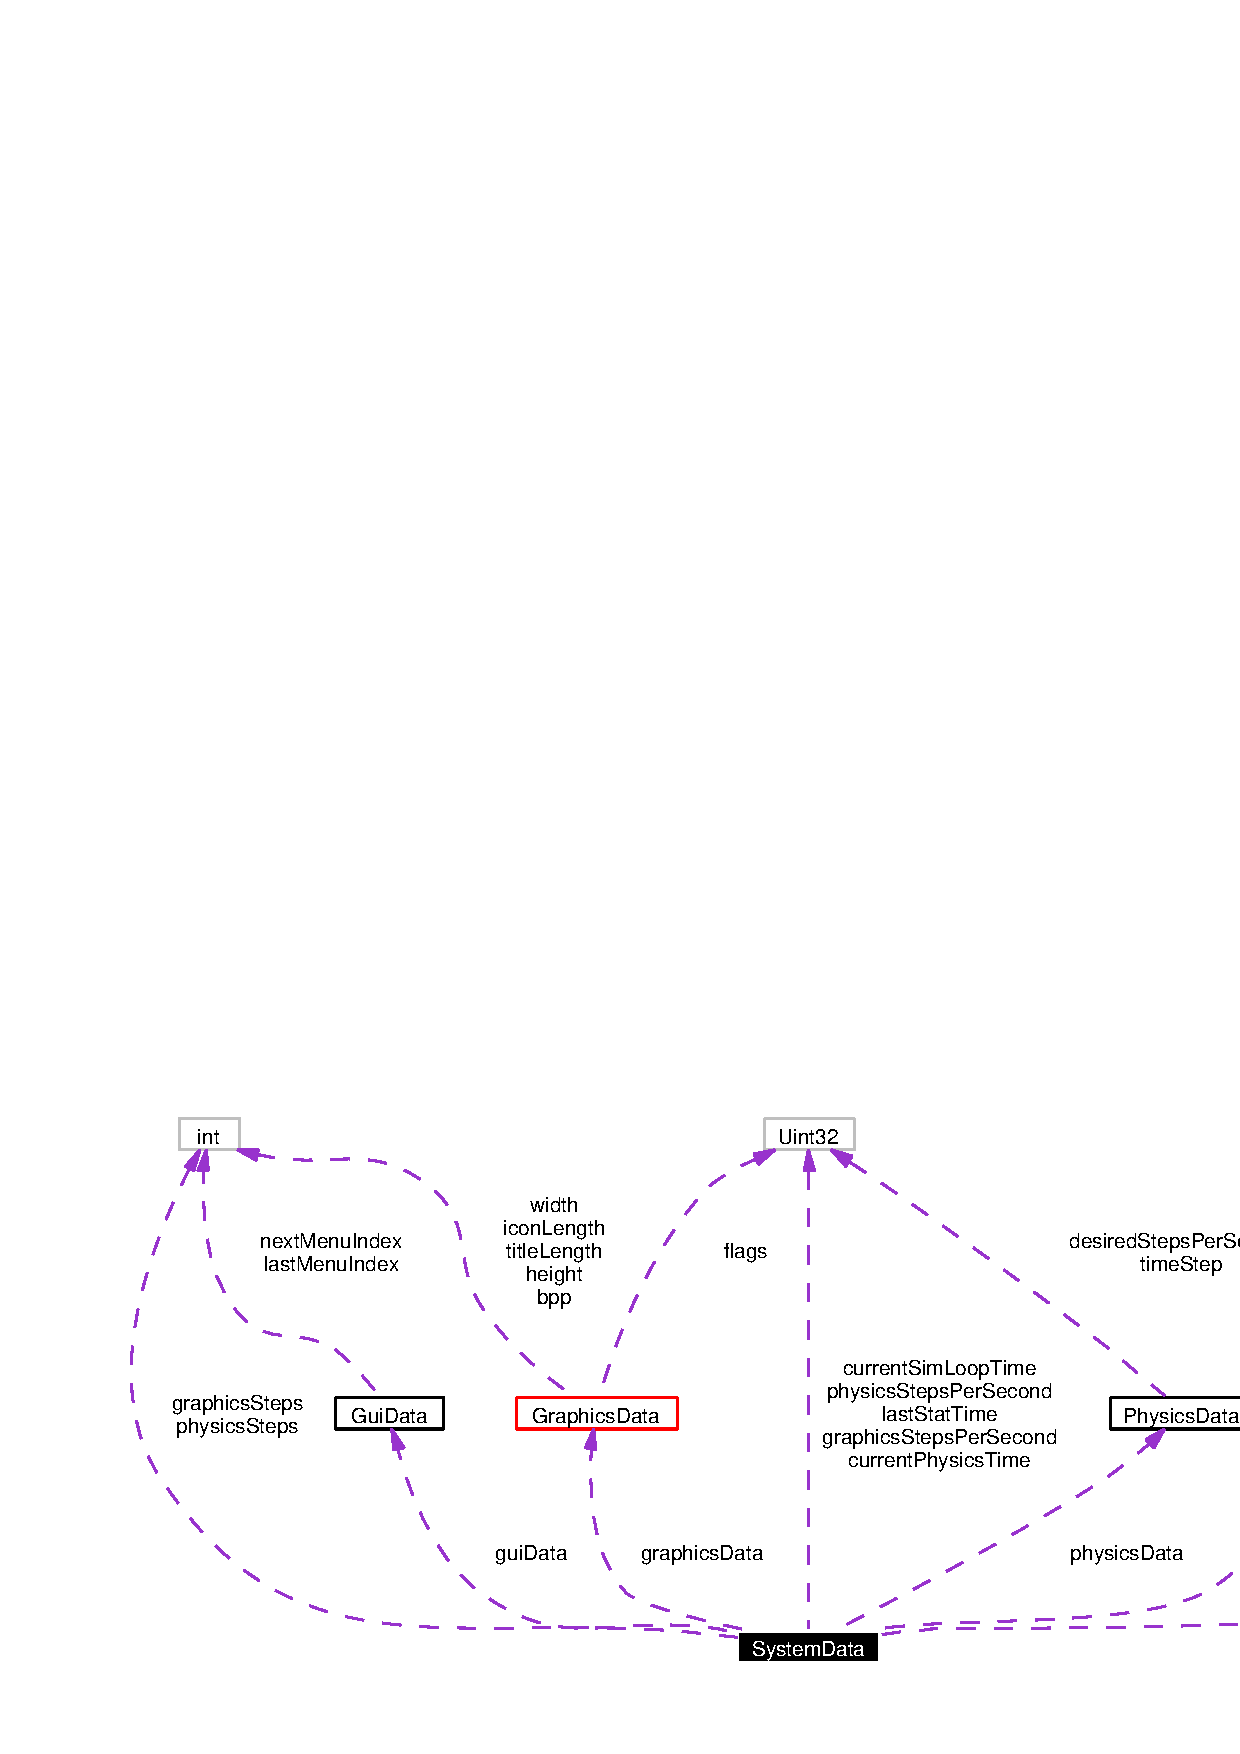
\includegraphics[width=397pt]{classSystemData__coll__graph}
\end{center}
\end{figure}
\subsection*{Public Member Functions}
\begin{CompactItemize}
\item 
bool {\bf can\-Main\-Loop\-Run} (void)
\item 
bool {\bf can\-Sim\-Loop\-Run} (void)
\item 
bool {\bf can\-Gui\-Loop\-Run} (void)
\item 
void {\bf enable\-Main\-Loop} (void)
\item 
void {\bf enable\-Sim\-Loop} (void)
\item 
void {\bf enable\-Gui\-Loop} (void)
\item 
void {\bf disable\-Main\-Loop} (void)
\item 
void {\bf disable\-Sim\-Loop} (void)
\item 
void {\bf disable\-Gui\-Loop} (void)
\end{CompactItemize}
\subsection*{Public Attributes}
\begin{CompactItemize}
\item 
{\bf Graphics\-Data} {\bf graphics\-Data}
\item 
{\bf Input\-Data} {\bf input\-Data}
\item 
{\bf Physics\-Data} {\bf physics\-Data}
\item 
{\bf Gui\-Data} {\bf gui\-Data}
\item 
Uint32 {\bf current\-Sim\-Loop\-Time}
\item 
Uint32 {\bf current\-Physics\-Time}
\item 
Uint32 {\bf last\-Stat\-Time}
\item 
int {\bf physics\-Steps}
\item 
Uint32 {\bf physics\-Steps\-Per\-Second}
\item 
int {\bf graphics\-Steps}
\item 
Uint32 {\bf graphics\-Steps\-Per\-Second}
\end{CompactItemize}
\subsection*{Private Attributes}
\begin{CompactItemize}
\item 
bool {\bf main\-Loop\-Enabled}
\item 
bool {\bf sim\-Loop\-Enabled}
\item 
bool {\bf gui\-Loop\-Enabled}
\end{CompactItemize}


\subsection{Member Function Documentation}
\index{SystemData@{System\-Data}!canGuiLoopRun@{canGuiLoopRun}}
\index{canGuiLoopRun@{canGuiLoopRun}!SystemData@{System\-Data}}
\subsubsection{\setlength{\rightskip}{0pt plus 5cm}bool System\-Data::can\-Gui\-Loop\-Run (void)}\label{classSystemData_a2}


\index{SystemData@{System\-Data}!canMainLoopRun@{canMainLoopRun}}
\index{canMainLoopRun@{canMainLoopRun}!SystemData@{System\-Data}}
\subsubsection{\setlength{\rightskip}{0pt plus 5cm}bool System\-Data::can\-Main\-Loop\-Run (void)}\label{classSystemData_a0}


\index{SystemData@{System\-Data}!canSimLoopRun@{canSimLoopRun}}
\index{canSimLoopRun@{canSimLoopRun}!SystemData@{System\-Data}}
\subsubsection{\setlength{\rightskip}{0pt plus 5cm}bool System\-Data::can\-Sim\-Loop\-Run (void)}\label{classSystemData_a1}


\index{SystemData@{System\-Data}!disableGuiLoop@{disableGuiLoop}}
\index{disableGuiLoop@{disableGuiLoop}!SystemData@{System\-Data}}
\subsubsection{\setlength{\rightskip}{0pt plus 5cm}void System\-Data::disable\-Gui\-Loop (void)}\label{classSystemData_a8}


\index{SystemData@{System\-Data}!disableMainLoop@{disableMainLoop}}
\index{disableMainLoop@{disableMainLoop}!SystemData@{System\-Data}}
\subsubsection{\setlength{\rightskip}{0pt plus 5cm}void System\-Data::disable\-Main\-Loop (void)}\label{classSystemData_a6}


\index{SystemData@{System\-Data}!disableSimLoop@{disableSimLoop}}
\index{disableSimLoop@{disableSimLoop}!SystemData@{System\-Data}}
\subsubsection{\setlength{\rightskip}{0pt plus 5cm}void System\-Data::disable\-Sim\-Loop (void)}\label{classSystemData_a7}


\index{SystemData@{System\-Data}!enableGuiLoop@{enableGuiLoop}}
\index{enableGuiLoop@{enableGuiLoop}!SystemData@{System\-Data}}
\subsubsection{\setlength{\rightskip}{0pt plus 5cm}void System\-Data::enable\-Gui\-Loop (void)}\label{classSystemData_a5}


\index{SystemData@{System\-Data}!enableMainLoop@{enableMainLoop}}
\index{enableMainLoop@{enableMainLoop}!SystemData@{System\-Data}}
\subsubsection{\setlength{\rightskip}{0pt plus 5cm}void System\-Data::enable\-Main\-Loop (void)}\label{classSystemData_a3}


\index{SystemData@{System\-Data}!enableSimLoop@{enableSimLoop}}
\index{enableSimLoop@{enableSimLoop}!SystemData@{System\-Data}}
\subsubsection{\setlength{\rightskip}{0pt plus 5cm}void System\-Data::enable\-Sim\-Loop (void)}\label{classSystemData_a4}




\subsection{Member Data Documentation}
\index{SystemData@{System\-Data}!currentPhysicsTime@{currentPhysicsTime}}
\index{currentPhysicsTime@{currentPhysicsTime}!SystemData@{System\-Data}}
\subsubsection{\setlength{\rightskip}{0pt plus 5cm}Uint32 {\bf System\-Data::current\-Physics\-Time}}\label{classSystemData_o5}


\index{SystemData@{System\-Data}!currentSimLoopTime@{currentSimLoopTime}}
\index{currentSimLoopTime@{currentSimLoopTime}!SystemData@{System\-Data}}
\subsubsection{\setlength{\rightskip}{0pt plus 5cm}Uint32 {\bf System\-Data::current\-Sim\-Loop\-Time}}\label{classSystemData_o4}


\index{SystemData@{System\-Data}!graphicsData@{graphicsData}}
\index{graphicsData@{graphicsData}!SystemData@{System\-Data}}
\subsubsection{\setlength{\rightskip}{0pt plus 5cm}struct {\bf Graphics\-Data} {\bf System\-Data::graphics\-Data}}\label{classSystemData_o0}


\index{SystemData@{System\-Data}!graphicsSteps@{graphicsSteps}}
\index{graphicsSteps@{graphicsSteps}!SystemData@{System\-Data}}
\subsubsection{\setlength{\rightskip}{0pt plus 5cm}int {\bf System\-Data::graphics\-Steps}}\label{classSystemData_o9}


\index{SystemData@{System\-Data}!graphicsStepsPerSecond@{graphicsStepsPerSecond}}
\index{graphicsStepsPerSecond@{graphicsStepsPerSecond}!SystemData@{System\-Data}}
\subsubsection{\setlength{\rightskip}{0pt plus 5cm}Uint32 {\bf System\-Data::graphics\-Steps\-Per\-Second}}\label{classSystemData_o10}


\index{SystemData@{System\-Data}!guiData@{guiData}}
\index{guiData@{guiData}!SystemData@{System\-Data}}
\subsubsection{\setlength{\rightskip}{0pt plus 5cm}struct {\bf Gui\-Data} {\bf System\-Data::gui\-Data}}\label{classSystemData_o3}


\index{SystemData@{System\-Data}!guiLoopEnabled@{guiLoopEnabled}}
\index{guiLoopEnabled@{guiLoopEnabled}!SystemData@{System\-Data}}
\subsubsection{\setlength{\rightskip}{0pt plus 5cm}bool {\bf System\-Data::gui\-Loop\-Enabled}\hspace{0.3cm}{\tt  [private]}}\label{classSystemData_r2}


\index{SystemData@{System\-Data}!inputData@{inputData}}
\index{inputData@{inputData}!SystemData@{System\-Data}}
\subsubsection{\setlength{\rightskip}{0pt plus 5cm}struct {\bf Input\-Data} {\bf System\-Data::input\-Data}}\label{classSystemData_o1}


\index{SystemData@{System\-Data}!lastStatTime@{lastStatTime}}
\index{lastStatTime@{lastStatTime}!SystemData@{System\-Data}}
\subsubsection{\setlength{\rightskip}{0pt plus 5cm}Uint32 {\bf System\-Data::last\-Stat\-Time}}\label{classSystemData_o6}


\index{SystemData@{System\-Data}!mainLoopEnabled@{mainLoopEnabled}}
\index{mainLoopEnabled@{mainLoopEnabled}!SystemData@{System\-Data}}
\subsubsection{\setlength{\rightskip}{0pt plus 5cm}bool {\bf System\-Data::main\-Loop\-Enabled}\hspace{0.3cm}{\tt  [private]}}\label{classSystemData_r0}


\index{SystemData@{System\-Data}!physicsData@{physicsData}}
\index{physicsData@{physicsData}!SystemData@{System\-Data}}
\subsubsection{\setlength{\rightskip}{0pt plus 5cm}struct {\bf Physics\-Data} {\bf System\-Data::physics\-Data}}\label{classSystemData_o2}


\index{SystemData@{System\-Data}!physicsSteps@{physicsSteps}}
\index{physicsSteps@{physicsSteps}!SystemData@{System\-Data}}
\subsubsection{\setlength{\rightskip}{0pt plus 5cm}int {\bf System\-Data::physics\-Steps}}\label{classSystemData_o7}


\index{SystemData@{System\-Data}!physicsStepsPerSecond@{physicsStepsPerSecond}}
\index{physicsStepsPerSecond@{physicsStepsPerSecond}!SystemData@{System\-Data}}
\subsubsection{\setlength{\rightskip}{0pt plus 5cm}Uint32 {\bf System\-Data::physics\-Steps\-Per\-Second}}\label{classSystemData_o8}


\index{SystemData@{System\-Data}!simLoopEnabled@{simLoopEnabled}}
\index{simLoopEnabled@{simLoopEnabled}!SystemData@{System\-Data}}
\subsubsection{\setlength{\rightskip}{0pt plus 5cm}bool {\bf System\-Data::sim\-Loop\-Enabled}\hspace{0.3cm}{\tt  [private]}}\label{classSystemData_r1}




The documentation for this class was generated from the following files:\begin{CompactItemize}
\item 
src/{\bf system.hpp}\item 
src/{\bf system.cpp}\end{CompactItemize}

\section{Test\-Window Class Reference}
\label{classTestWindow}\index{TestWindow@{TestWindow}}
Inheritance diagram for Test\-Window::\begin{figure}[H]
\begin{center}
\leavevmode
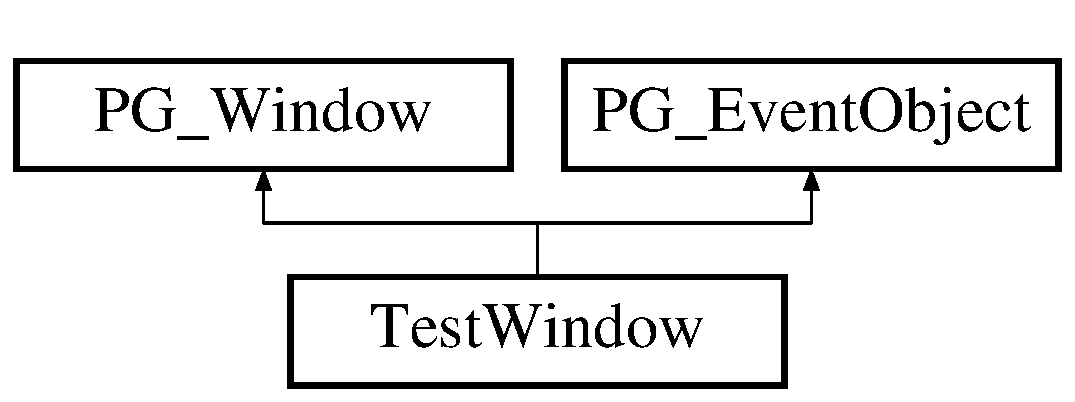
\includegraphics[height=2cm]{classTestWindow}
\end{center}
\end{figure}
Collaboration diagram for Test\-Window:\begin{figure}[H]
\begin{center}
\leavevmode
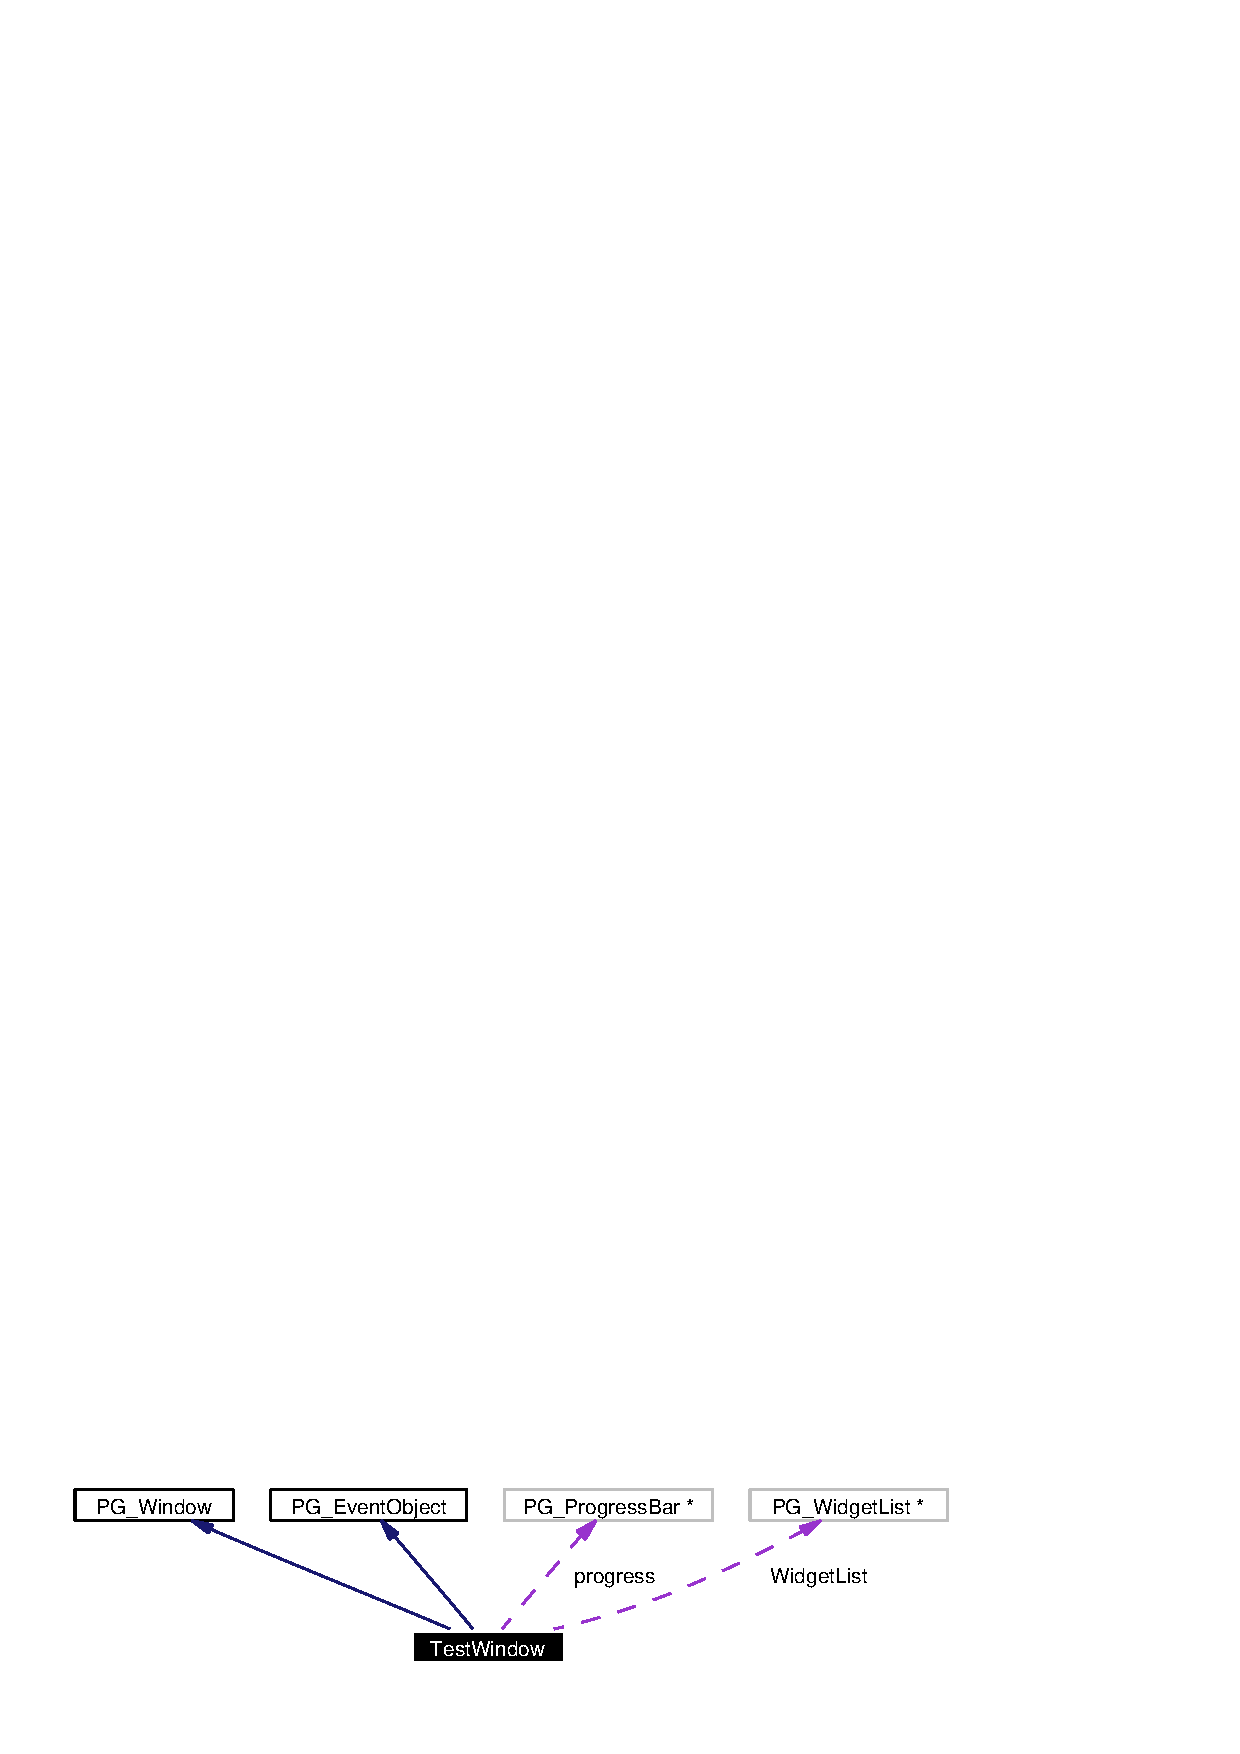
\includegraphics[width=236pt]{classTestWindow__coll__graph}
\end{center}
\end{figure}
\subsection*{Public Member Functions}
\begin{CompactItemize}
\item 
{\bf Test\-Window} (PG\_\-Widget $\ast$parent, const PG\_\-Rect \&r, char $\ast$windowtext)
\item 
virtual {\bf $\sim$Test\-Window} ()
\item 
void {\bf Dummy} ()
\item 
bool {\bf event\-Scroll\-Pos} (int id, PG\_\-Widget $\ast$widget, unsigned long data)
\item 
bool {\bf event\-Scroll\-Track} (int id, PG\_\-Widget $\ast$widget, unsigned long data)
\end{CompactItemize}
\subsection*{Private Attributes}
\begin{CompactItemize}
\item 
PG\_\-Progress\-Bar $\ast$ {\bf progress}
\item 
PG\_\-Widget\-List $\ast$ {\bf Widget\-List}
\end{CompactItemize}


\subsection{Constructor \& Destructor Documentation}
\index{TestWindow@{Test\-Window}!TestWindow@{TestWindow}}
\index{TestWindow@{TestWindow}!TestWindow@{Test\-Window}}
\subsubsection{\setlength{\rightskip}{0pt plus 5cm}Test\-Window::Test\-Window (PG\_\-Widget $\ast$ {\em parent}, const PG\_\-Rect \& {\em r}, char $\ast$ {\em windowtext})}\label{classTestWindow_a0}


\index{TestWindow@{Test\-Window}!~TestWindow@{$\sim$TestWindow}}
\index{~TestWindow@{$\sim$TestWindow}!TestWindow@{Test\-Window}}
\subsubsection{\setlength{\rightskip}{0pt plus 5cm}virtual Test\-Window::$\sim${\bf Test\-Window} ()\hspace{0.3cm}{\tt  [inline, virtual]}}\label{classTestWindow_a1}




\subsection{Member Function Documentation}
\index{TestWindow@{Test\-Window}!Dummy@{Dummy}}
\index{Dummy@{Dummy}!TestWindow@{Test\-Window}}
\subsubsection{\setlength{\rightskip}{0pt plus 5cm}void Test\-Window::Dummy ()\hspace{0.3cm}{\tt  [inline]}}\label{classTestWindow_a2}


\index{TestWindow@{Test\-Window}!eventScrollPos@{eventScrollPos}}
\index{eventScrollPos@{eventScrollPos}!TestWindow@{Test\-Window}}
\subsubsection{\setlength{\rightskip}{0pt plus 5cm}bool Test\-Window::event\-Scroll\-Pos (int {\em id}, PG\_\-Widget $\ast$ {\em widget}, unsigned long {\em data})}\label{classTestWindow_a3}


\index{TestWindow@{Test\-Window}!eventScrollTrack@{eventScrollTrack}}
\index{eventScrollTrack@{eventScrollTrack}!TestWindow@{Test\-Window}}
\subsubsection{\setlength{\rightskip}{0pt plus 5cm}bool Test\-Window::event\-Scroll\-Track (int {\em id}, PG\_\-Widget $\ast$ {\em widget}, unsigned long {\em data})}\label{classTestWindow_a4}




\subsection{Member Data Documentation}
\index{TestWindow@{Test\-Window}!progress@{progress}}
\index{progress@{progress}!TestWindow@{Test\-Window}}
\subsubsection{\setlength{\rightskip}{0pt plus 5cm}PG\_\-Progress\-Bar$\ast$ {\bf Test\-Window::progress}\hspace{0.3cm}{\tt  [private]}}\label{classTestWindow_r0}


\index{TestWindow@{Test\-Window}!WidgetList@{WidgetList}}
\index{WidgetList@{WidgetList}!TestWindow@{Test\-Window}}
\subsubsection{\setlength{\rightskip}{0pt plus 5cm}PG\_\-Widget\-List$\ast$ {\bf Test\-Window::Widget\-List}\hspace{0.3cm}{\tt  [private]}}\label{classTestWindow_r1}




The documentation for this class was generated from the following file:\begin{CompactItemize}
\item 
src/gui/{\bf test\_\-paragui.cpp}\end{CompactItemize}

\section{World\-Data Class Reference}
\label{classWorldData}\index{WorldData@{WorldData}}
{\tt \#include $<$world.hpp$>$}

Collaboration diagram for World\-Data:\begin{figure}[H]
\begin{center}
\leavevmode
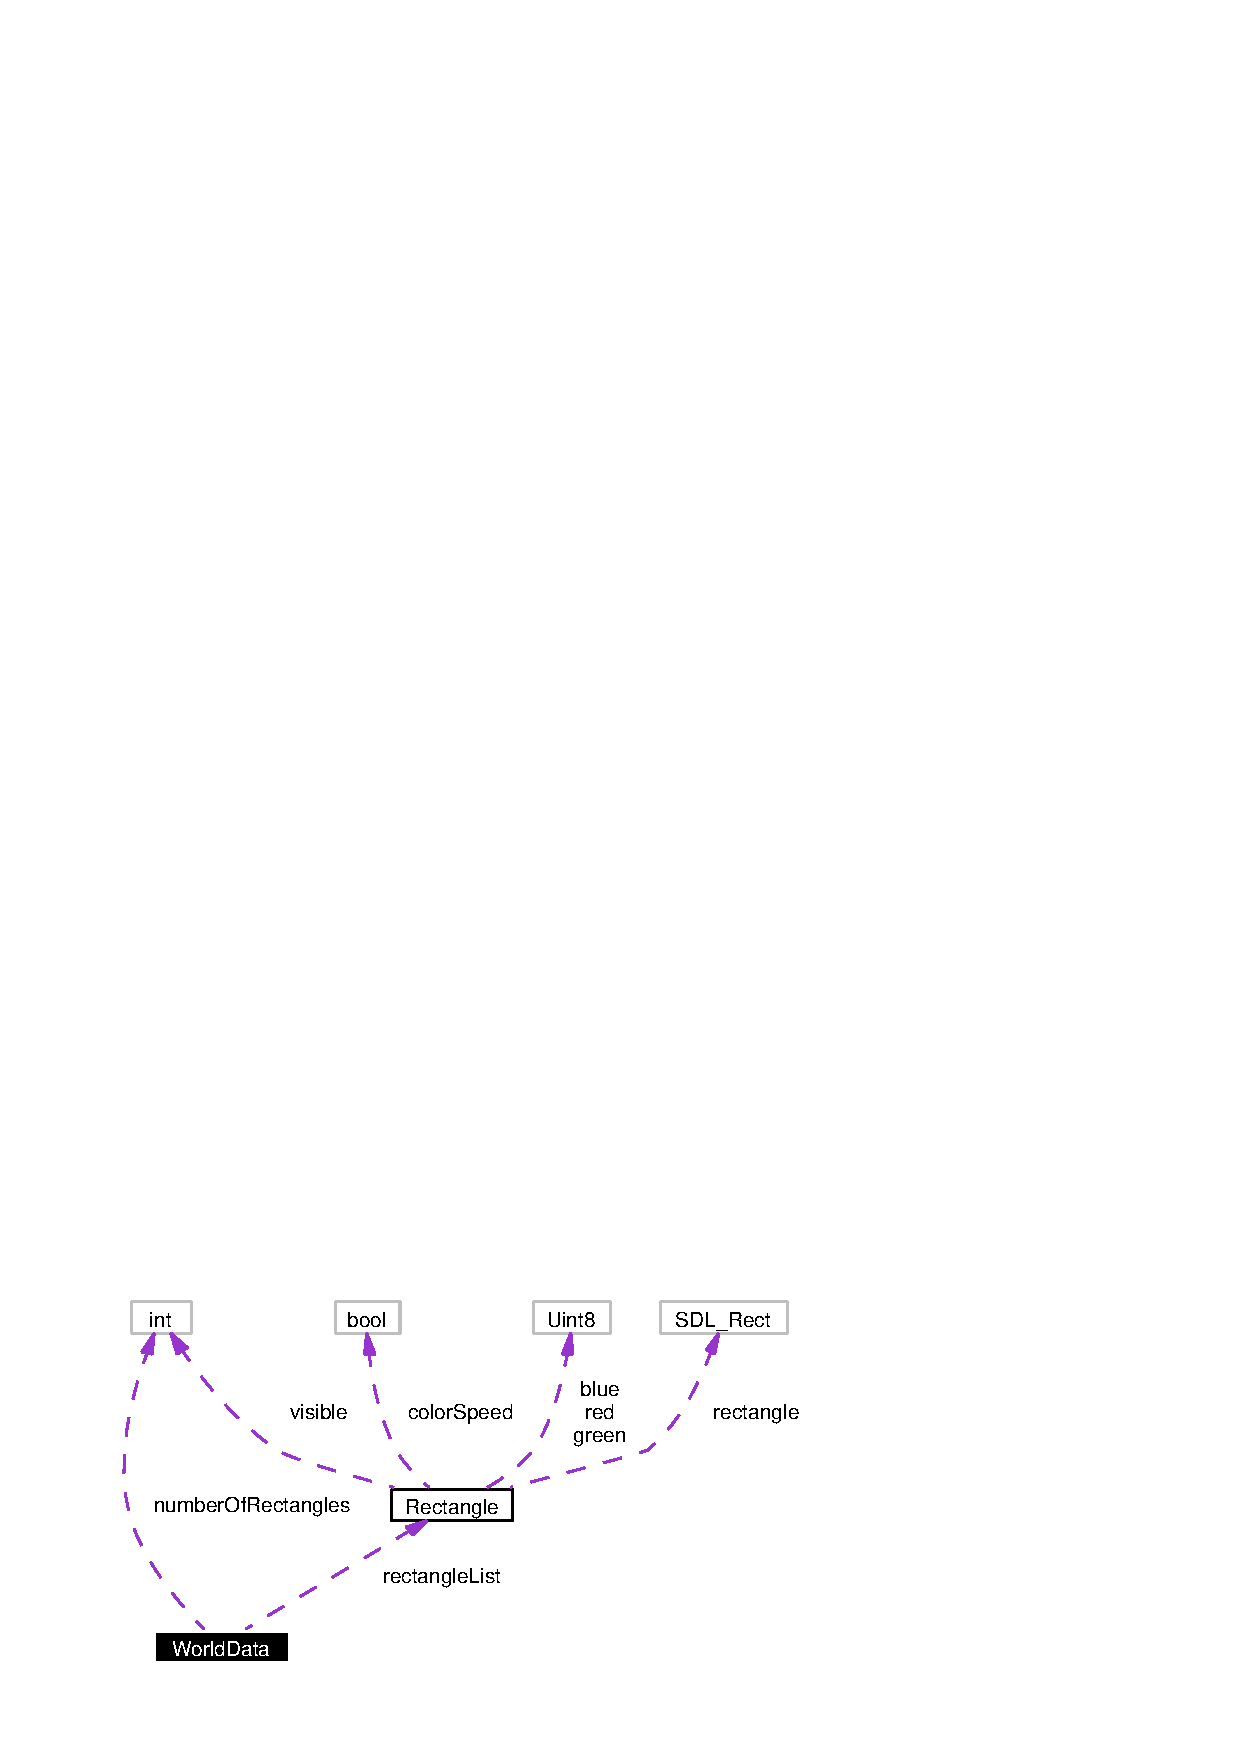
\includegraphics[width=201pt]{classWorldData__coll__graph}
\end{center}
\end{figure}
\subsection*{Public Attributes}
\begin{CompactItemize}
\item 
int {\bf number\-Of\-Rectangles}
\item 
{\bf Rectangle} $\ast$ {\bf rectangle\-List}
\end{CompactItemize}


\subsection{Member Data Documentation}
\index{WorldData@{World\-Data}!numberOfRectangles@{numberOfRectangles}}
\index{numberOfRectangles@{numberOfRectangles}!WorldData@{World\-Data}}
\subsubsection{\setlength{\rightskip}{0pt plus 5cm}int {\bf World\-Data::number\-Of\-Rectangles}}\label{classWorldData_o0}


\index{WorldData@{World\-Data}!rectangleList@{rectangleList}}
\index{rectangleList@{rectangleList}!WorldData@{World\-Data}}
\subsubsection{\setlength{\rightskip}{0pt plus 5cm}{\bf Rectangle}$\ast$ {\bf World\-Data::rectangle\-List}}\label{classWorldData_o1}




The documentation for this class was generated from the following file:\begin{CompactItemize}
\item 
src/{\bf world.hpp}\end{CompactItemize}

\chapter{Motorsport File Documentation}
\section{src/data/data\-Engine.cpp File Reference}
\label{dataEngine_8cpp}\index{src/data/dataEngine.cpp@{src/data/dataEngine.cpp}}
{\tt \#include \char`\"{}data\-Engine.hpp\char`\"{}}\par


Include dependency graph for data\-Engine.cpp:\begin{figure}[H]
\begin{center}
\leavevmode
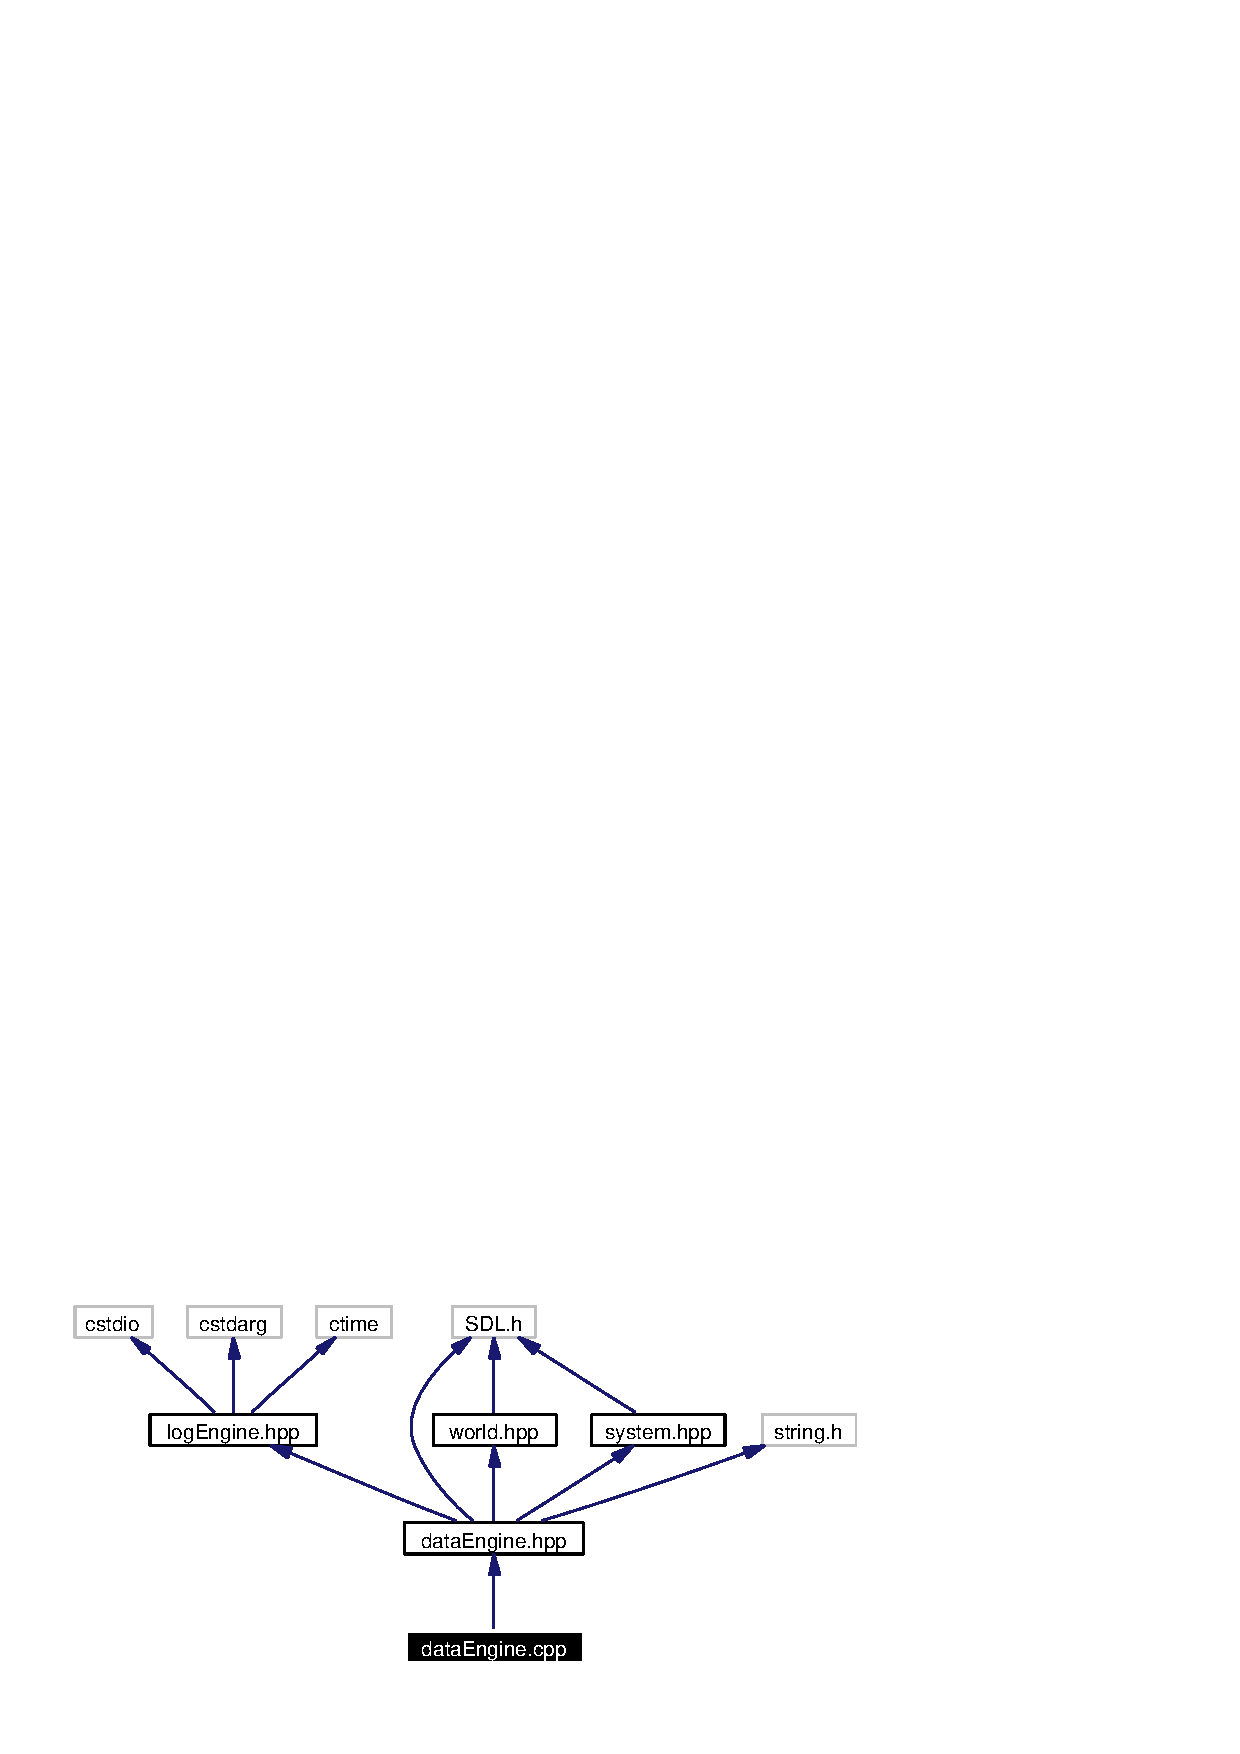
\includegraphics[width=205pt]{dataEngine_8cpp__incl}
\end{center}
\end{figure}

\section{src/data/data\-Engine.hpp File Reference}
\label{dataEngine_8hpp}\index{src/data/dataEngine.hpp@{src/data/dataEngine.hpp}}
{\tt \#include \char`\"{}log\-Engine.hpp\char`\"{}}\par
{\tt \#include \char`\"{}SDL.h\char`\"{}}\par
{\tt \#include \char`\"{}world.hpp\char`\"{}}\par
{\tt \#include \char`\"{}system.hpp\char`\"{}}\par
{\tt \#include $<$string.h$>$}\par


Include dependency graph for data\-Engine.hpp:\begin{figure}[H]
\begin{center}
\leavevmode
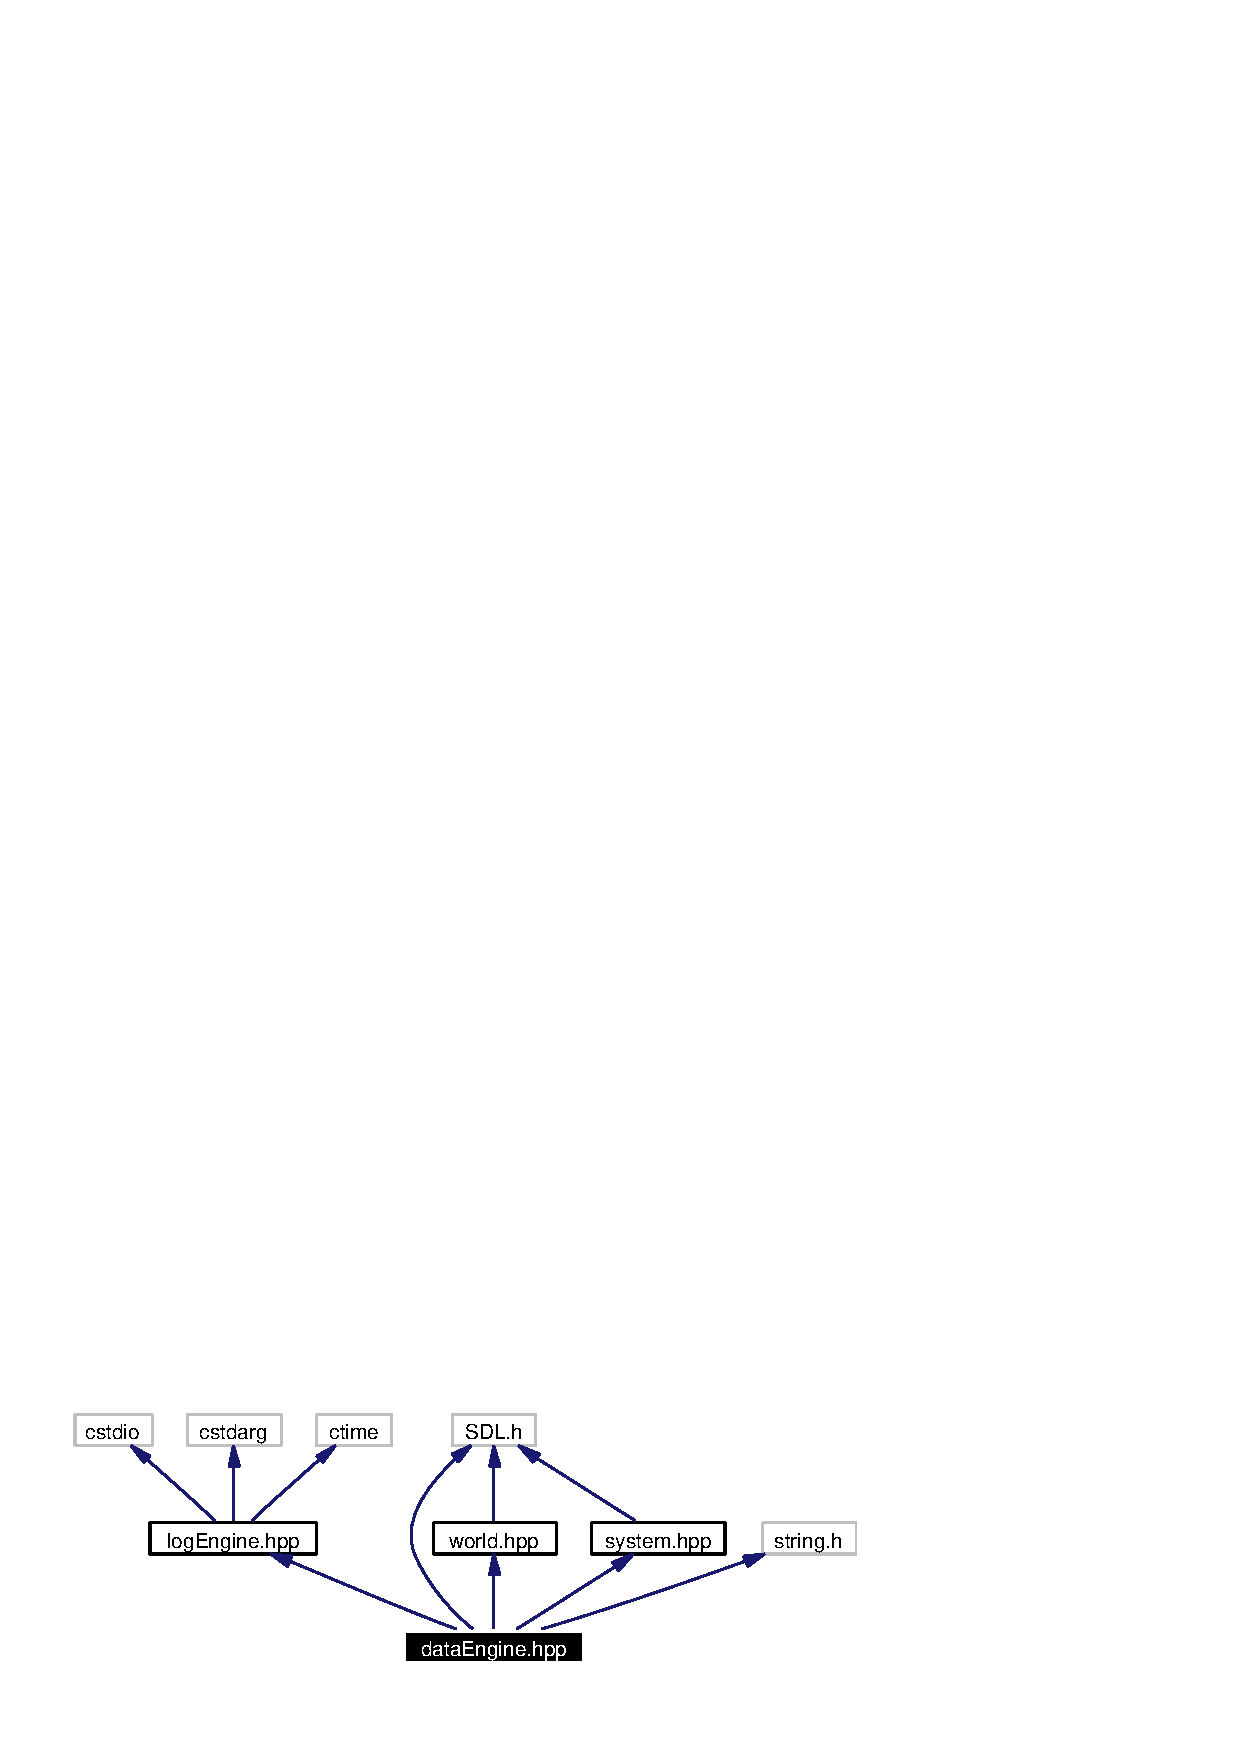
\includegraphics[width=205pt]{dataEngine_8hpp__incl}
\end{center}
\end{figure}


This graph shows which files directly or indirectly include this file:\begin{figure}[H]
\begin{center}
\leavevmode
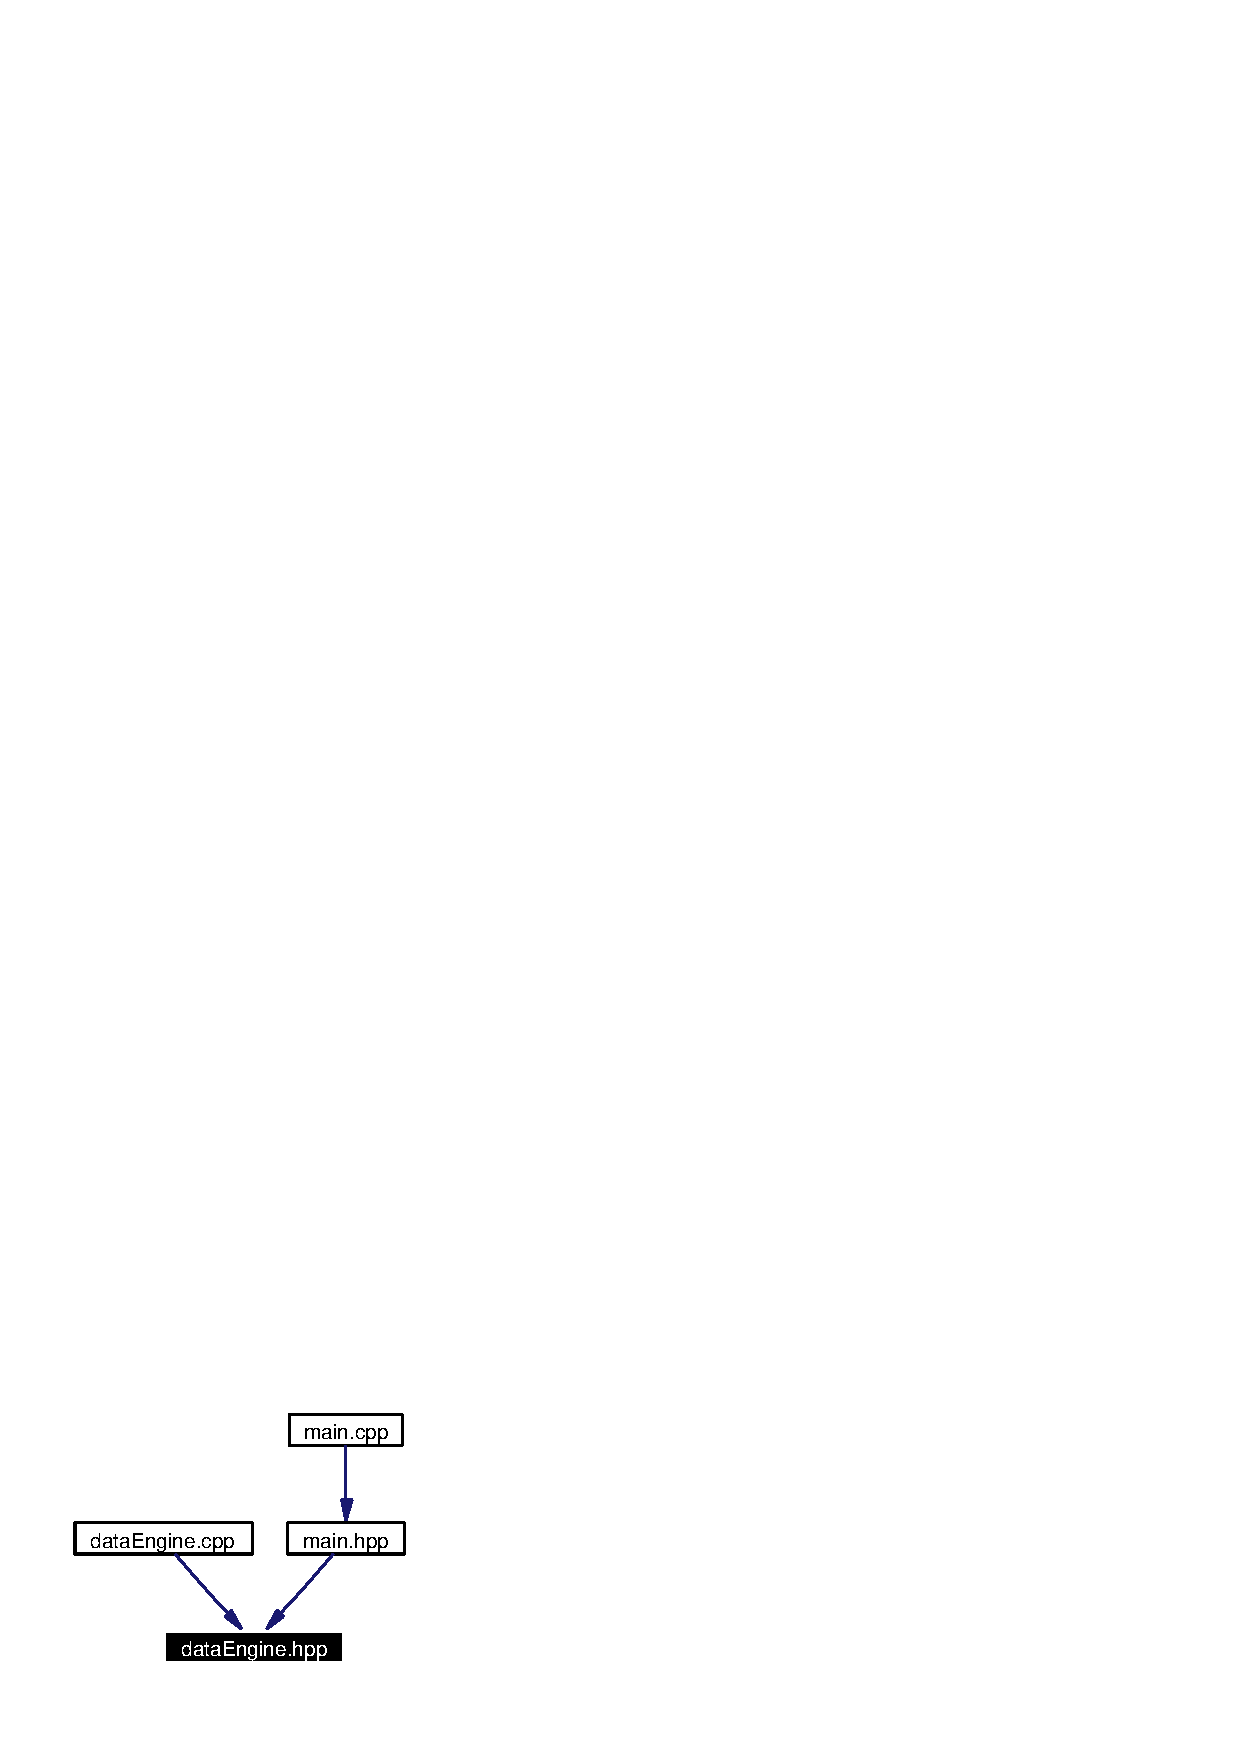
\includegraphics[width=97pt]{dataEngine_8hpp__dep__incl}
\end{center}
\end{figure}
\subsection*{Classes}
\begin{CompactItemize}
\item 
class {\bf Data\-Engine}
\end{CompactItemize}

\section{src/graphics/Example\-Application.h File Reference}
\label{ExampleApplication_8h}\index{src/graphics/ExampleApplication.h@{src/graphics/ExampleApplication.h}}
{\tt \#include \char`\"{}Ogre.h\char`\"{}}\par
{\tt \#include \char`\"{}Ogre\-Config\-File.h\char`\"{}}\par
{\tt \#include \char`\"{}Example\-Frame\-Listener.h\char`\"{}}\par


Include dependency graph for Example\-Application.h:\begin{figure}[H]
\begin{center}
\leavevmode
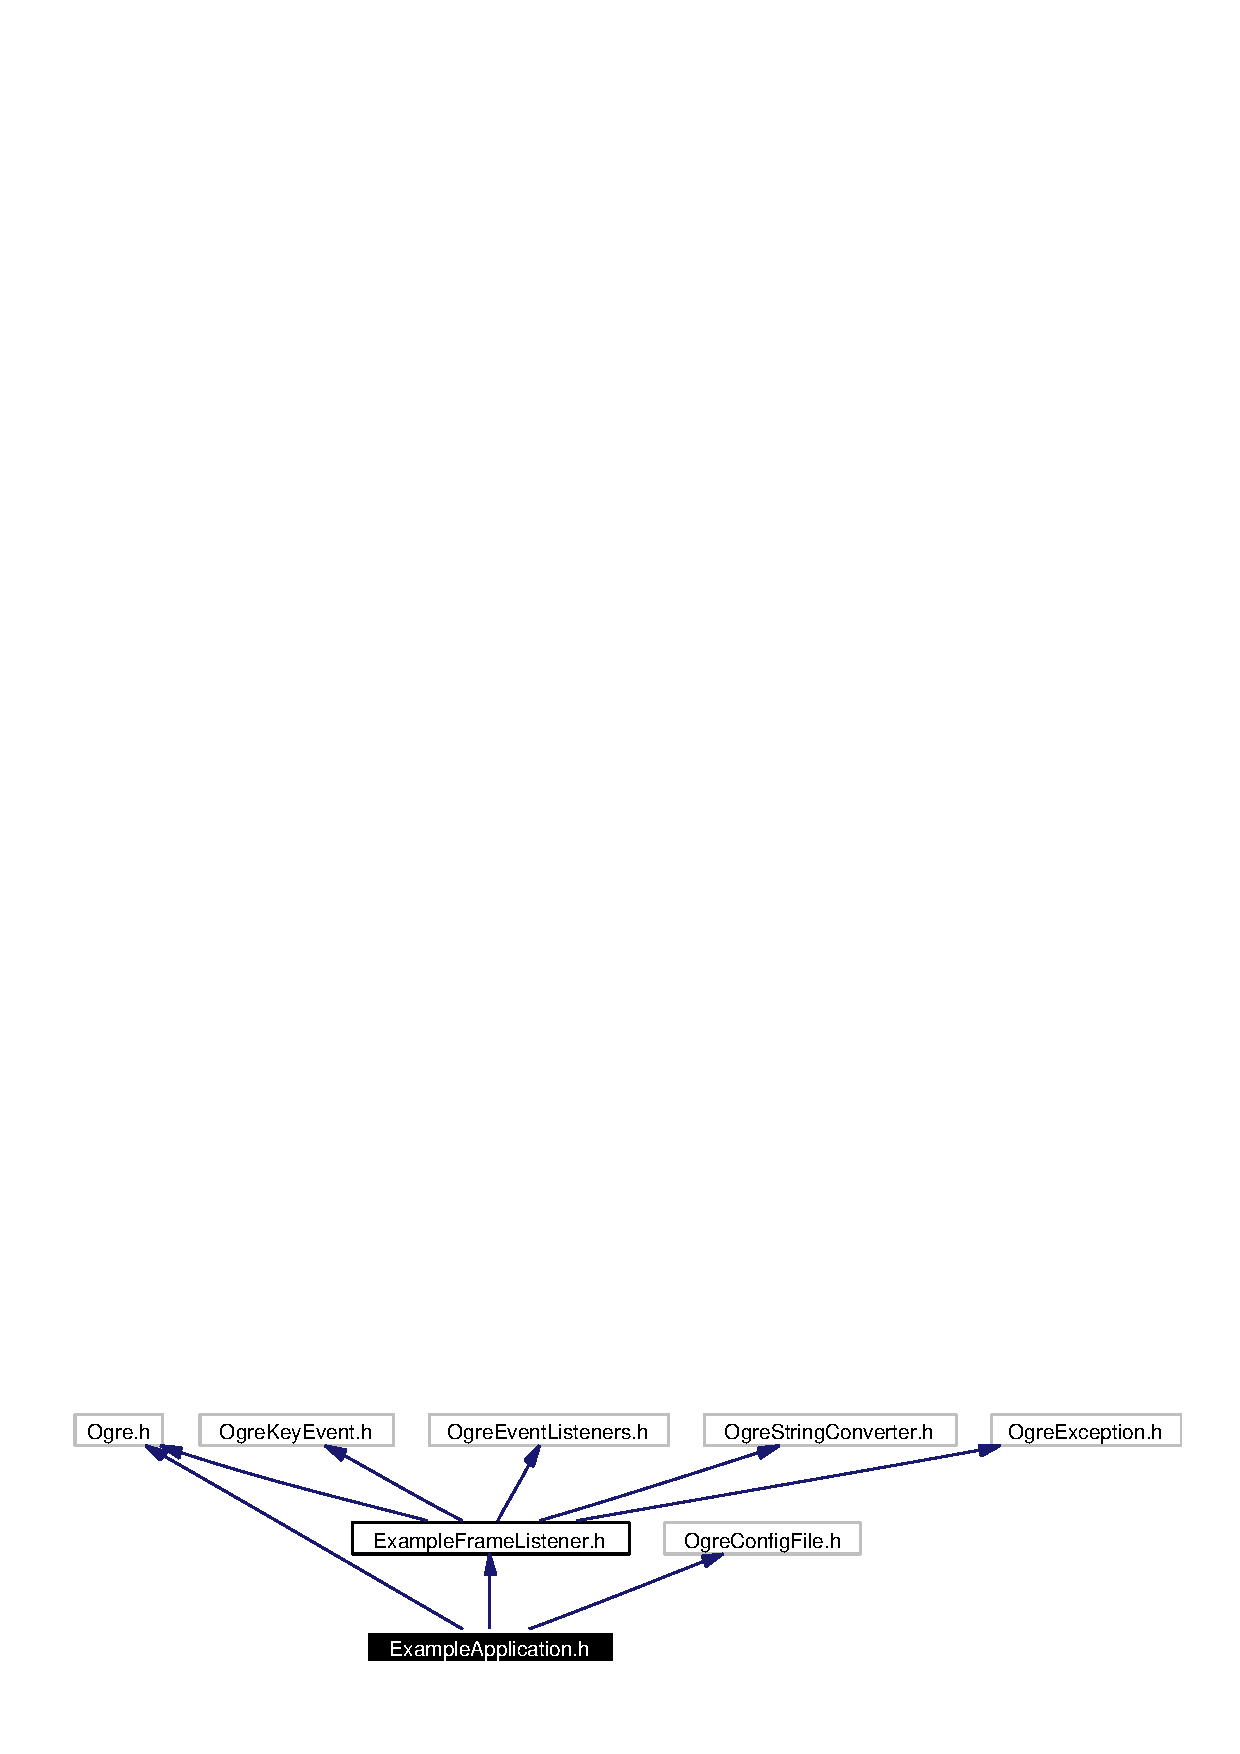
\includegraphics[width=283pt]{ExampleApplication_8h__incl}
\end{center}
\end{figure}


This graph shows which files directly or indirectly include this file:\begin{figure}[H]
\begin{center}
\leavevmode
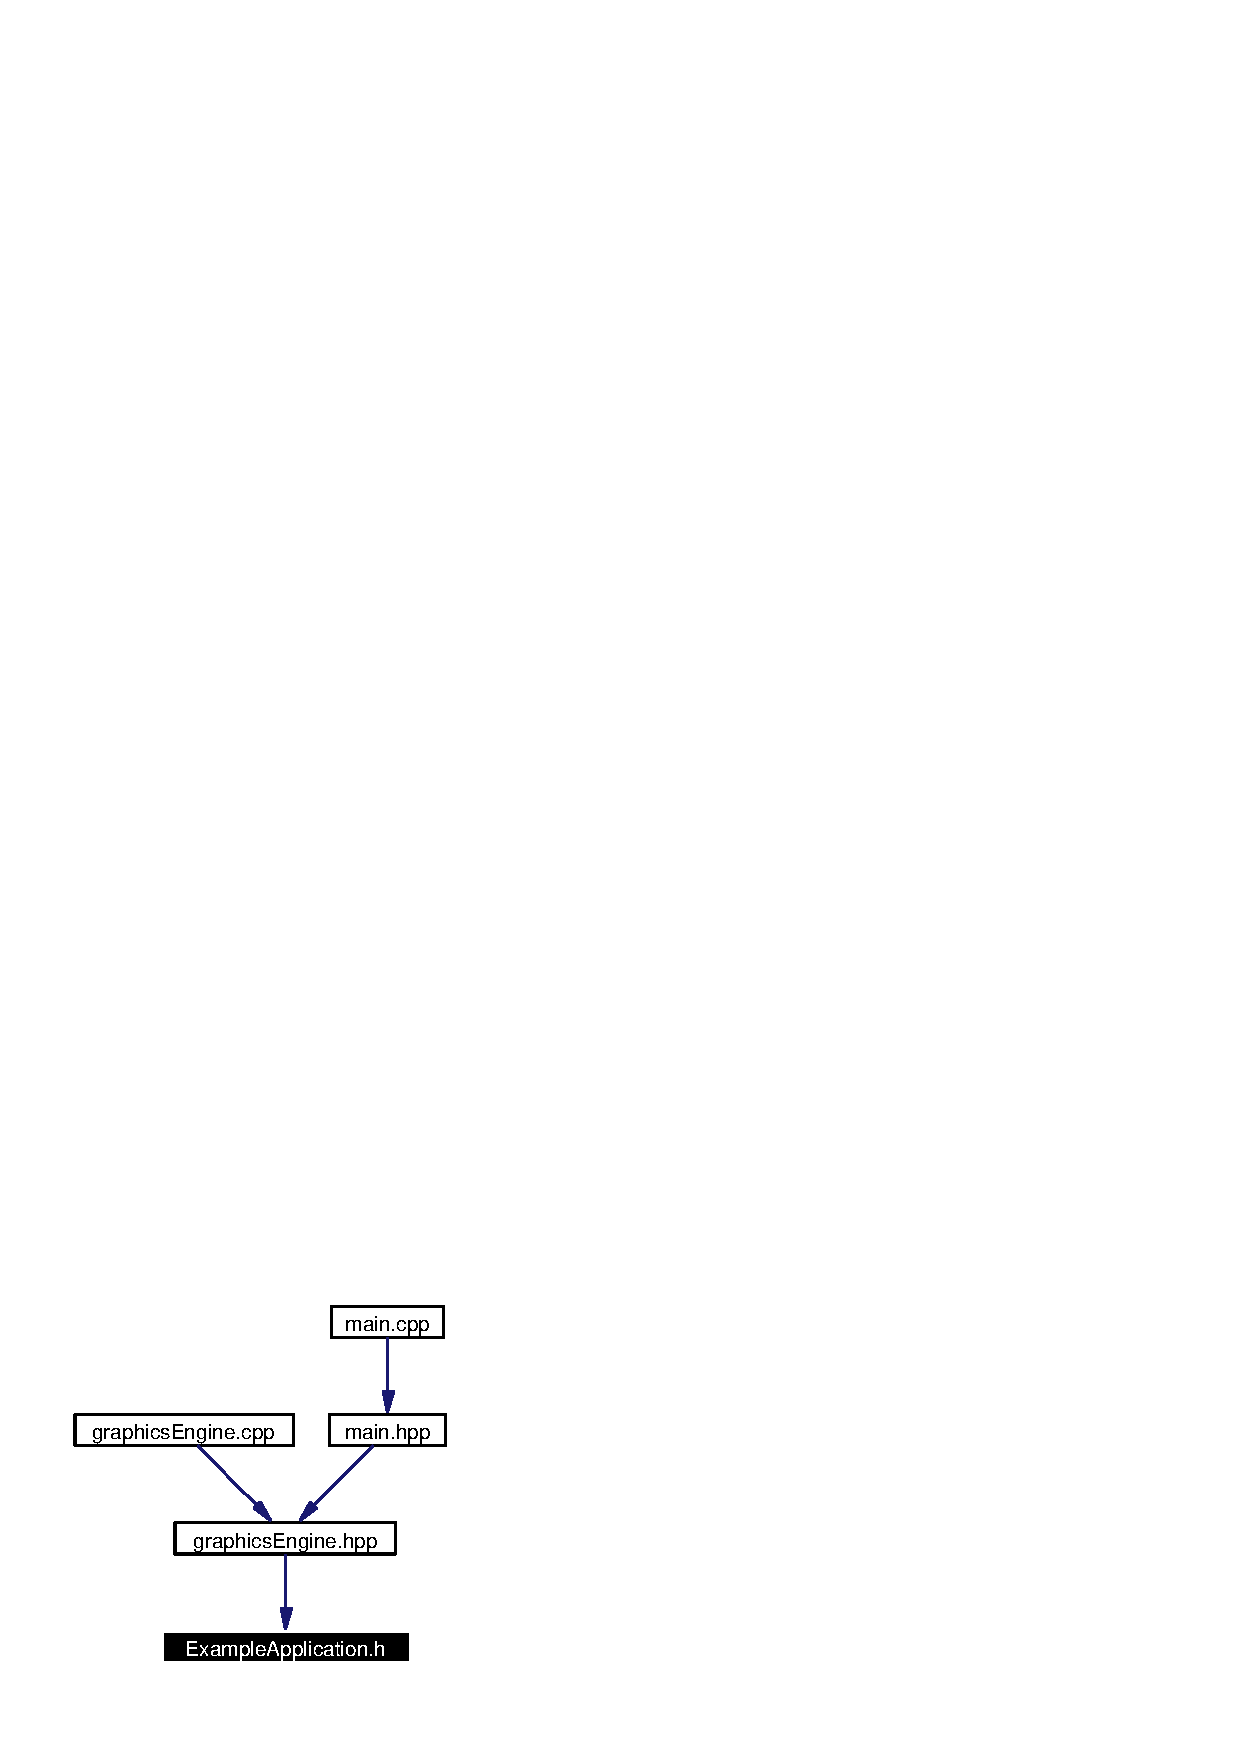
\includegraphics[width=107pt]{ExampleApplication_8h__dep__incl}
\end{center}
\end{figure}
\subsection*{Namespaces}
\begin{CompactItemize}
\item 
namespace {\bf Ogre}
\end{CompactItemize}
\subsection*{Classes}
\begin{CompactItemize}
\item 
class {\bf Example\-Application}
\end{CompactItemize}

\section{src/graphics/Example\-Frame\-Listener.h File Reference}
\label{ExampleFrameListener_8h}\index{src/graphics/ExampleFrameListener.h@{src/graphics/ExampleFrameListener.h}}
{\tt \#include \char`\"{}Ogre.h\char`\"{}}\par
{\tt \#include \char`\"{}Ogre\-Key\-Event.h\char`\"{}}\par
{\tt \#include \char`\"{}Ogre\-Event\-Listeners.h\char`\"{}}\par
{\tt \#include \char`\"{}Ogre\-String\-Converter.h\char`\"{}}\par
{\tt \#include \char`\"{}Ogre\-Exception.h\char`\"{}}\par


Include dependency graph for Example\-Frame\-Listener.h:\begin{figure}[H]
\begin{center}
\leavevmode
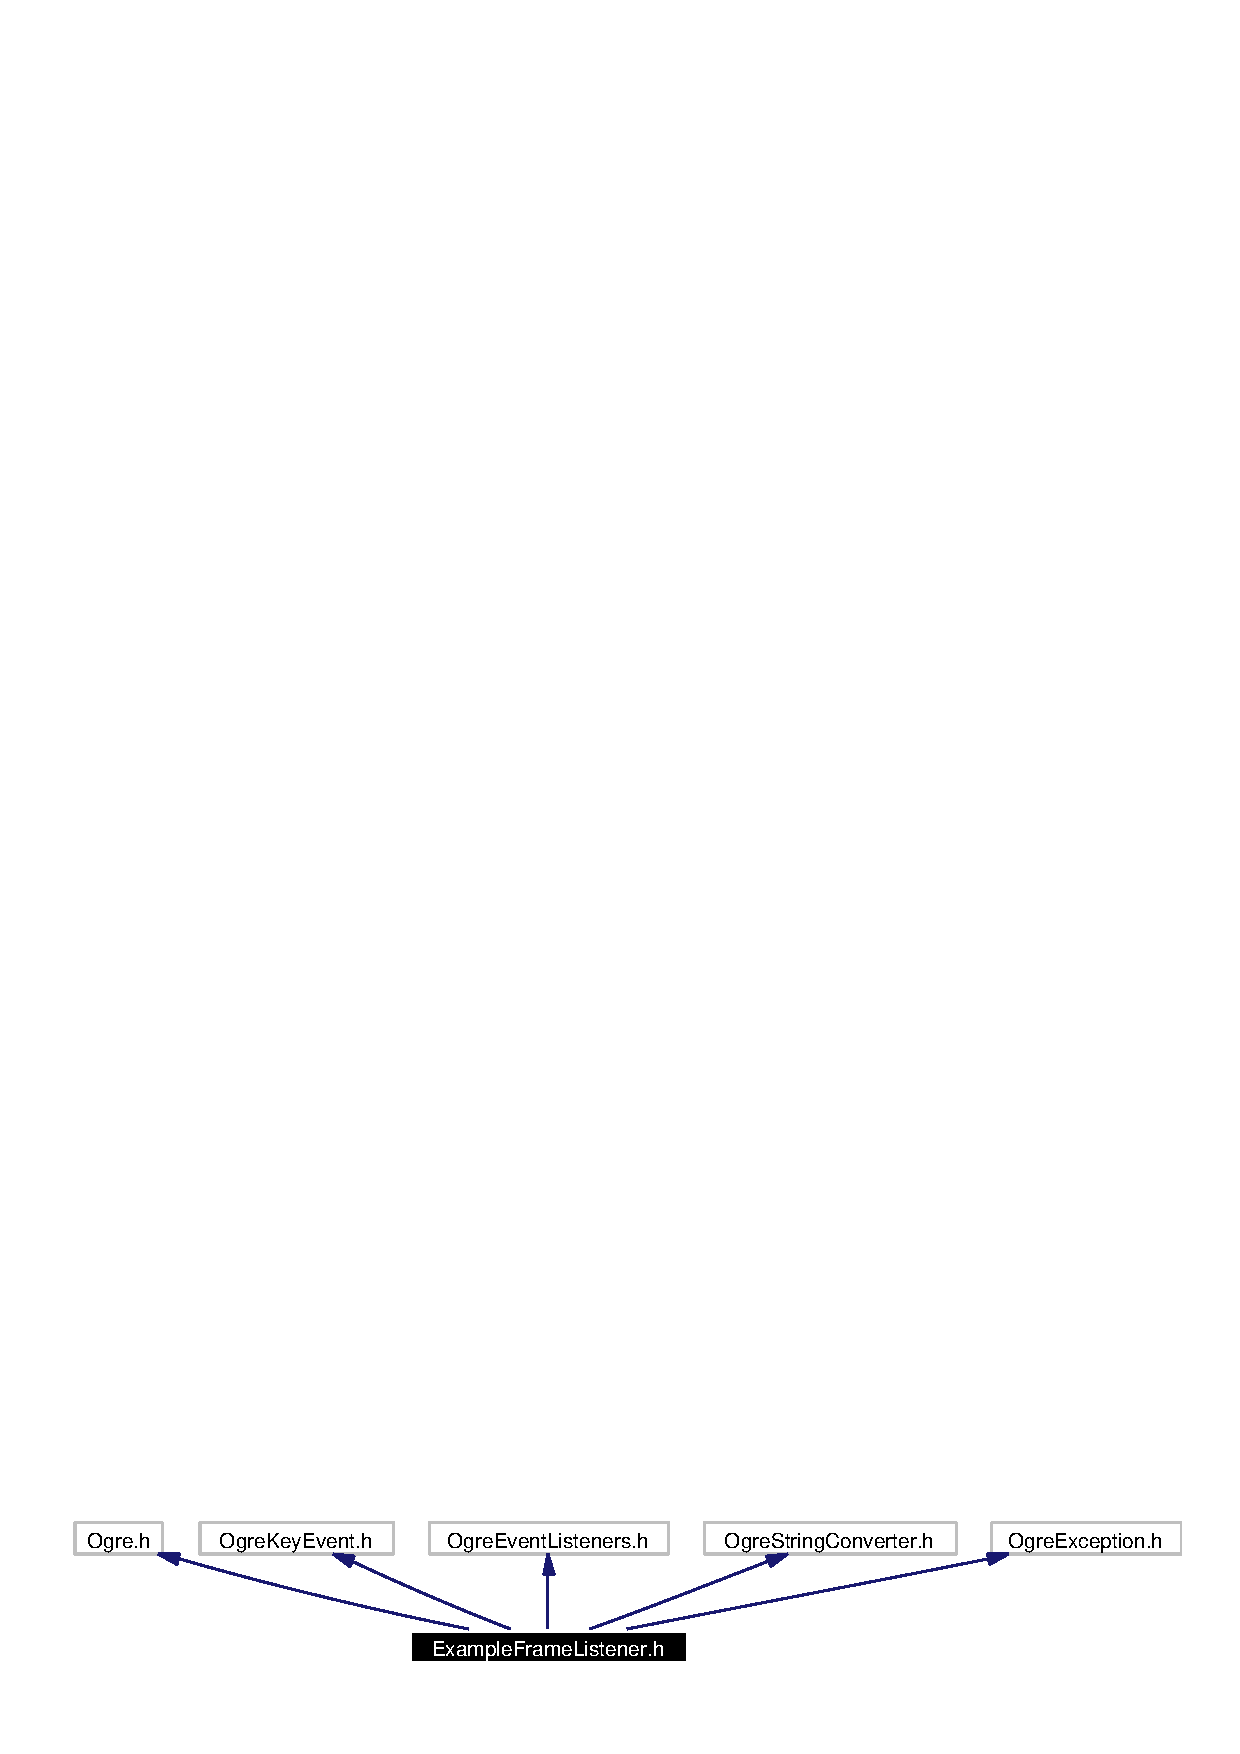
\includegraphics[width=283pt]{ExampleFrameListener_8h__incl}
\end{center}
\end{figure}


This graph shows which files directly or indirectly include this file:\begin{figure}[H]
\begin{center}
\leavevmode
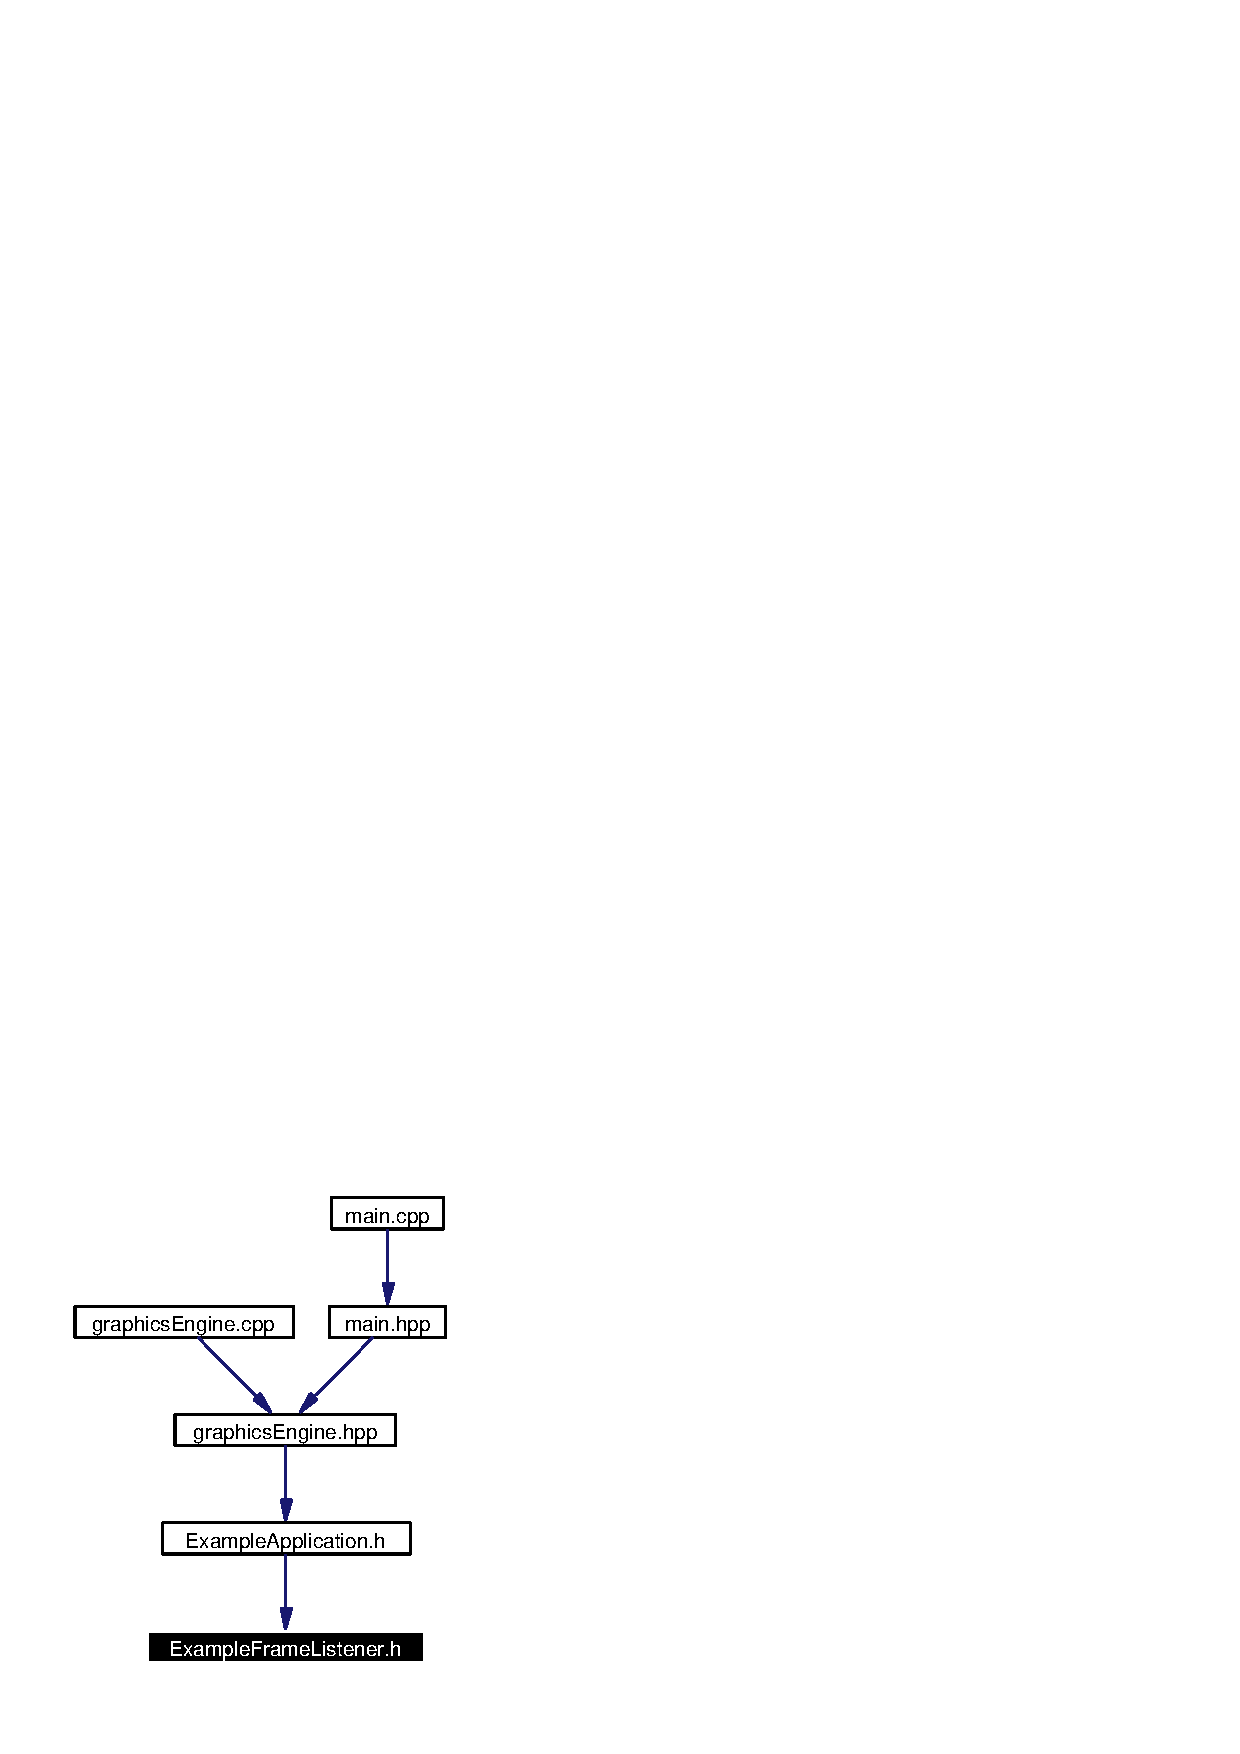
\includegraphics[width=107pt]{ExampleFrameListener_8h__dep__incl}
\end{center}
\end{figure}
\subsection*{Classes}
\begin{CompactItemize}
\item 
class {\bf Example\-Frame\-Listener}
\end{CompactItemize}

\section{src/graphics/graphics\-Engine.cpp File Reference}
\label{graphicsEngine_8cpp}\index{src/graphics/graphicsEngine.cpp@{src/graphics/graphicsEngine.cpp}}
{\tt \#include \char`\"{}system.hpp\char`\"{}}\par
{\tt \#include \char`\"{}world.hpp\char`\"{}}\par
{\tt \#include \char`\"{}graphics\-Engine.hpp\char`\"{}}\par
{\tt \#include $<$stdlib.h$>$}\par


Include dependency graph for graphics\-Engine.cpp:\begin{figure}[H]
\begin{center}
\leavevmode
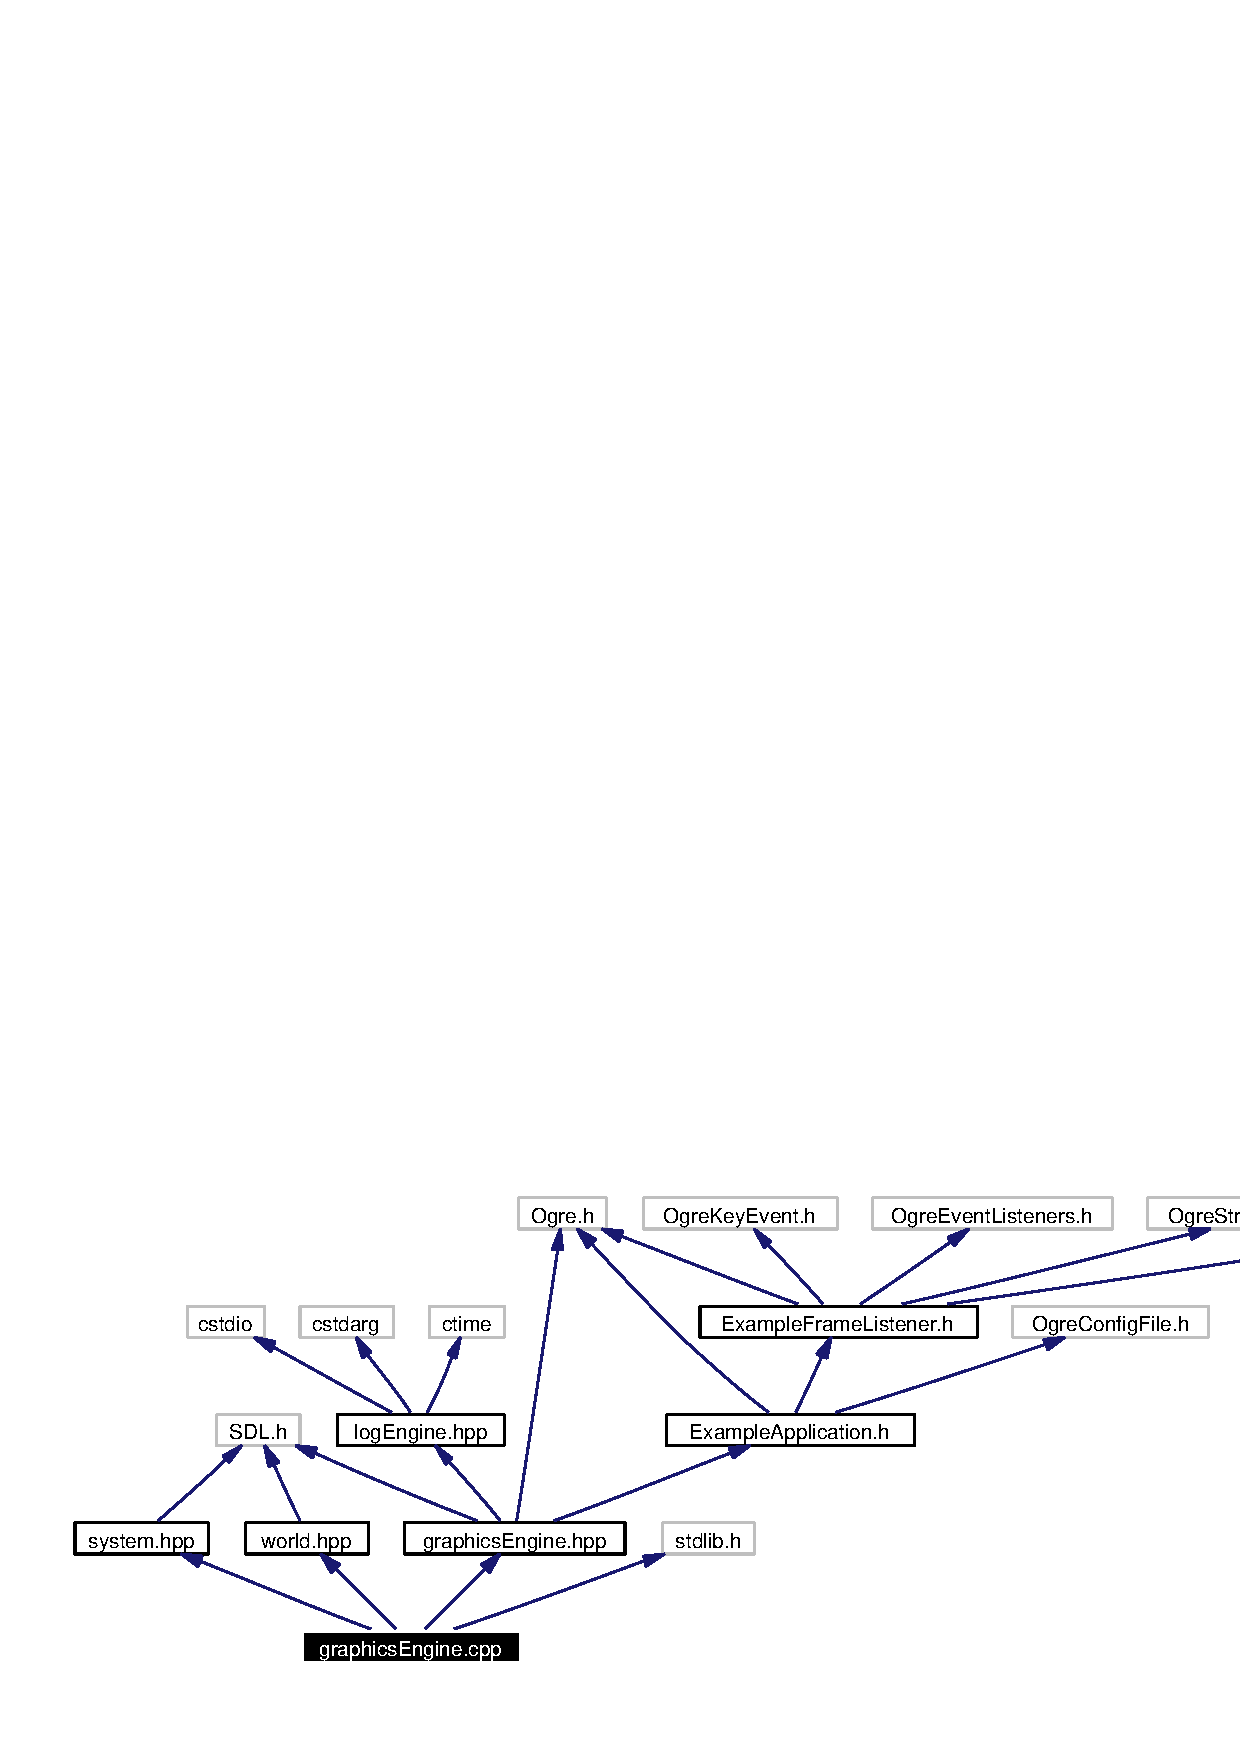
\includegraphics[width=390pt]{graphicsEngine_8cpp__incl}
\end{center}
\end{figure}

\section{src/graphics/graphics\-Engine.hpp File Reference}
\label{graphicsEngine_8hpp}\index{src/graphics/graphicsEngine.hpp@{src/graphics/graphicsEngine.hpp}}
{\tt \#include \char`\"{}log\-Engine.hpp\char`\"{}}\par
{\tt \#include \char`\"{}SDL.h\char`\"{}}\par
{\tt \#include \char`\"{}Ogre.h\char`\"{}}\par
{\tt \#include \char`\"{}Example\-Application.h\char`\"{}}\par


Include dependency graph for graphics\-Engine.hpp:\begin{figure}[H]
\begin{center}
\leavevmode
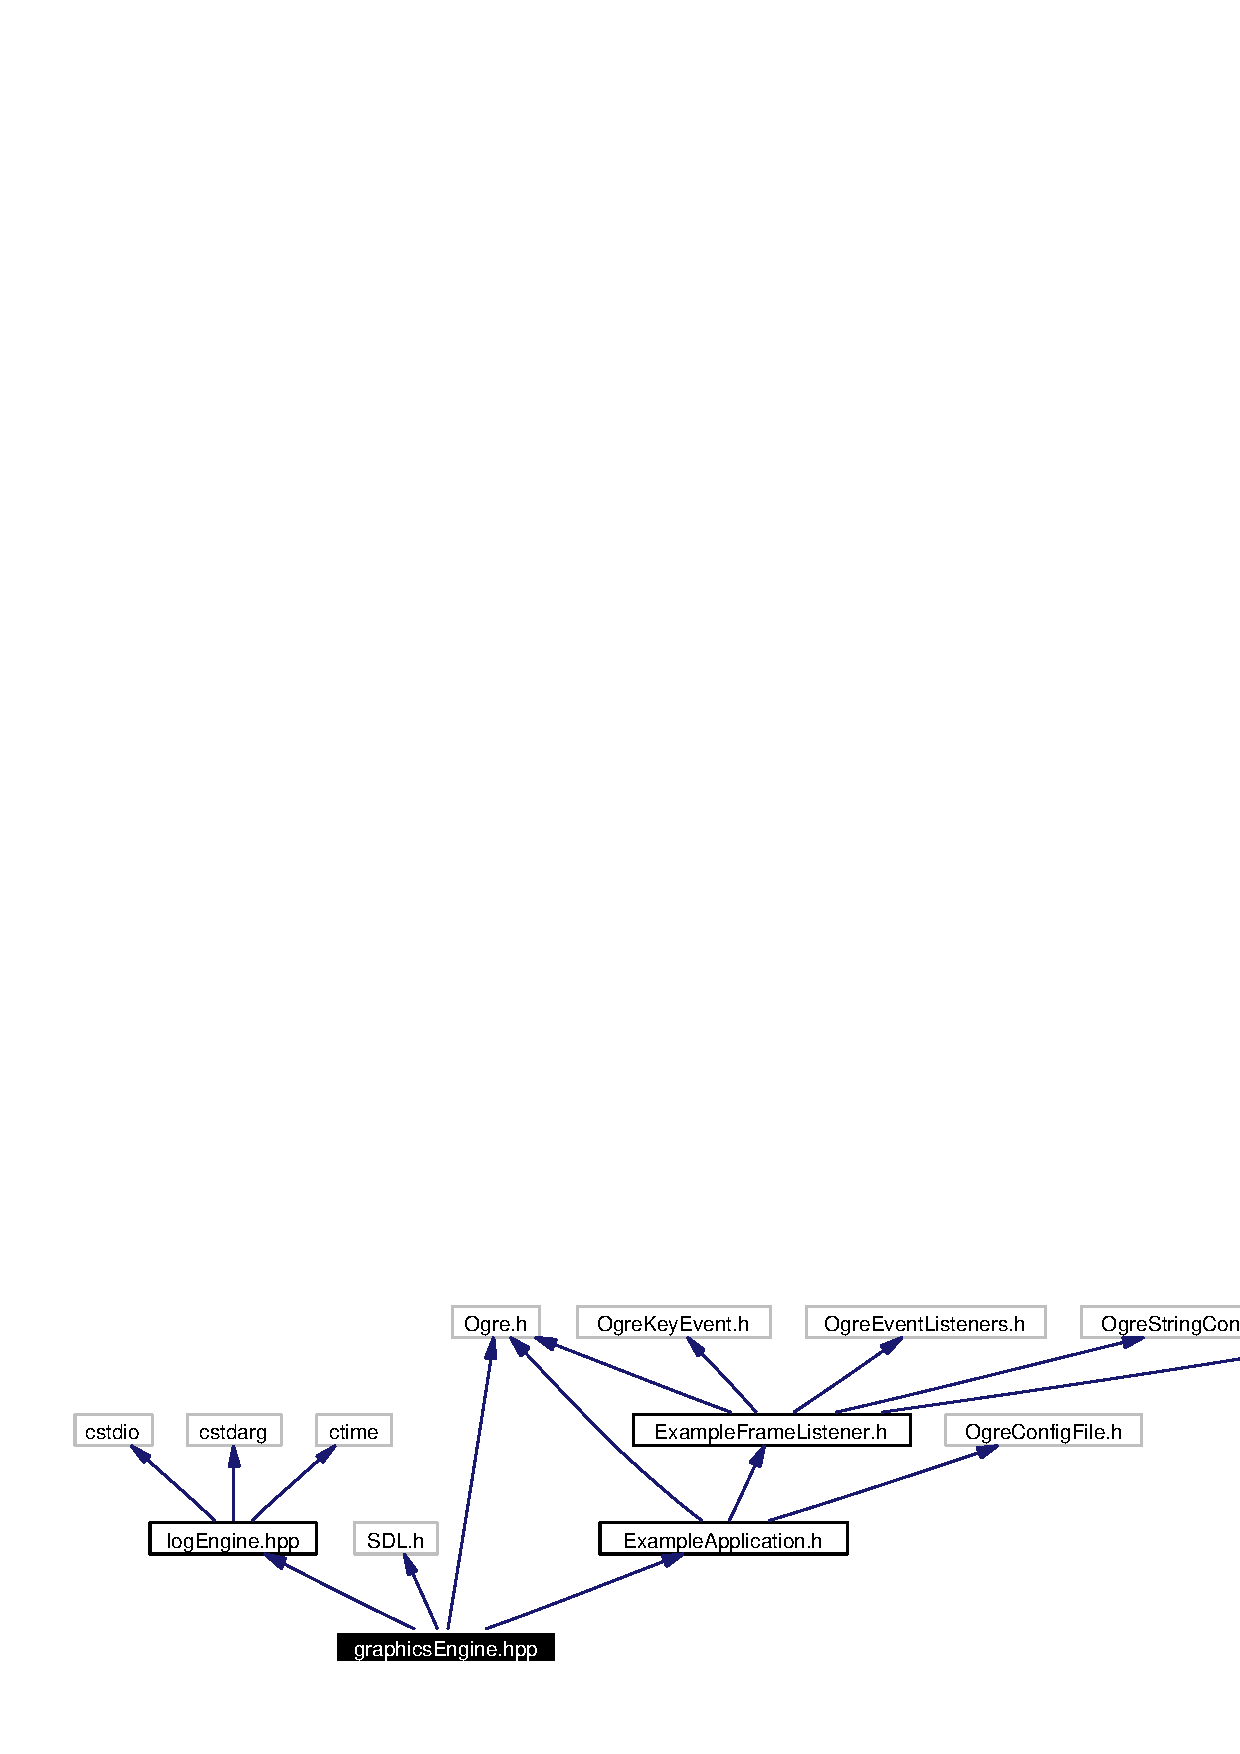
\includegraphics[width=374pt]{graphicsEngine_8hpp__incl}
\end{center}
\end{figure}


This graph shows which files directly or indirectly include this file:\begin{figure}[H]
\begin{center}
\leavevmode
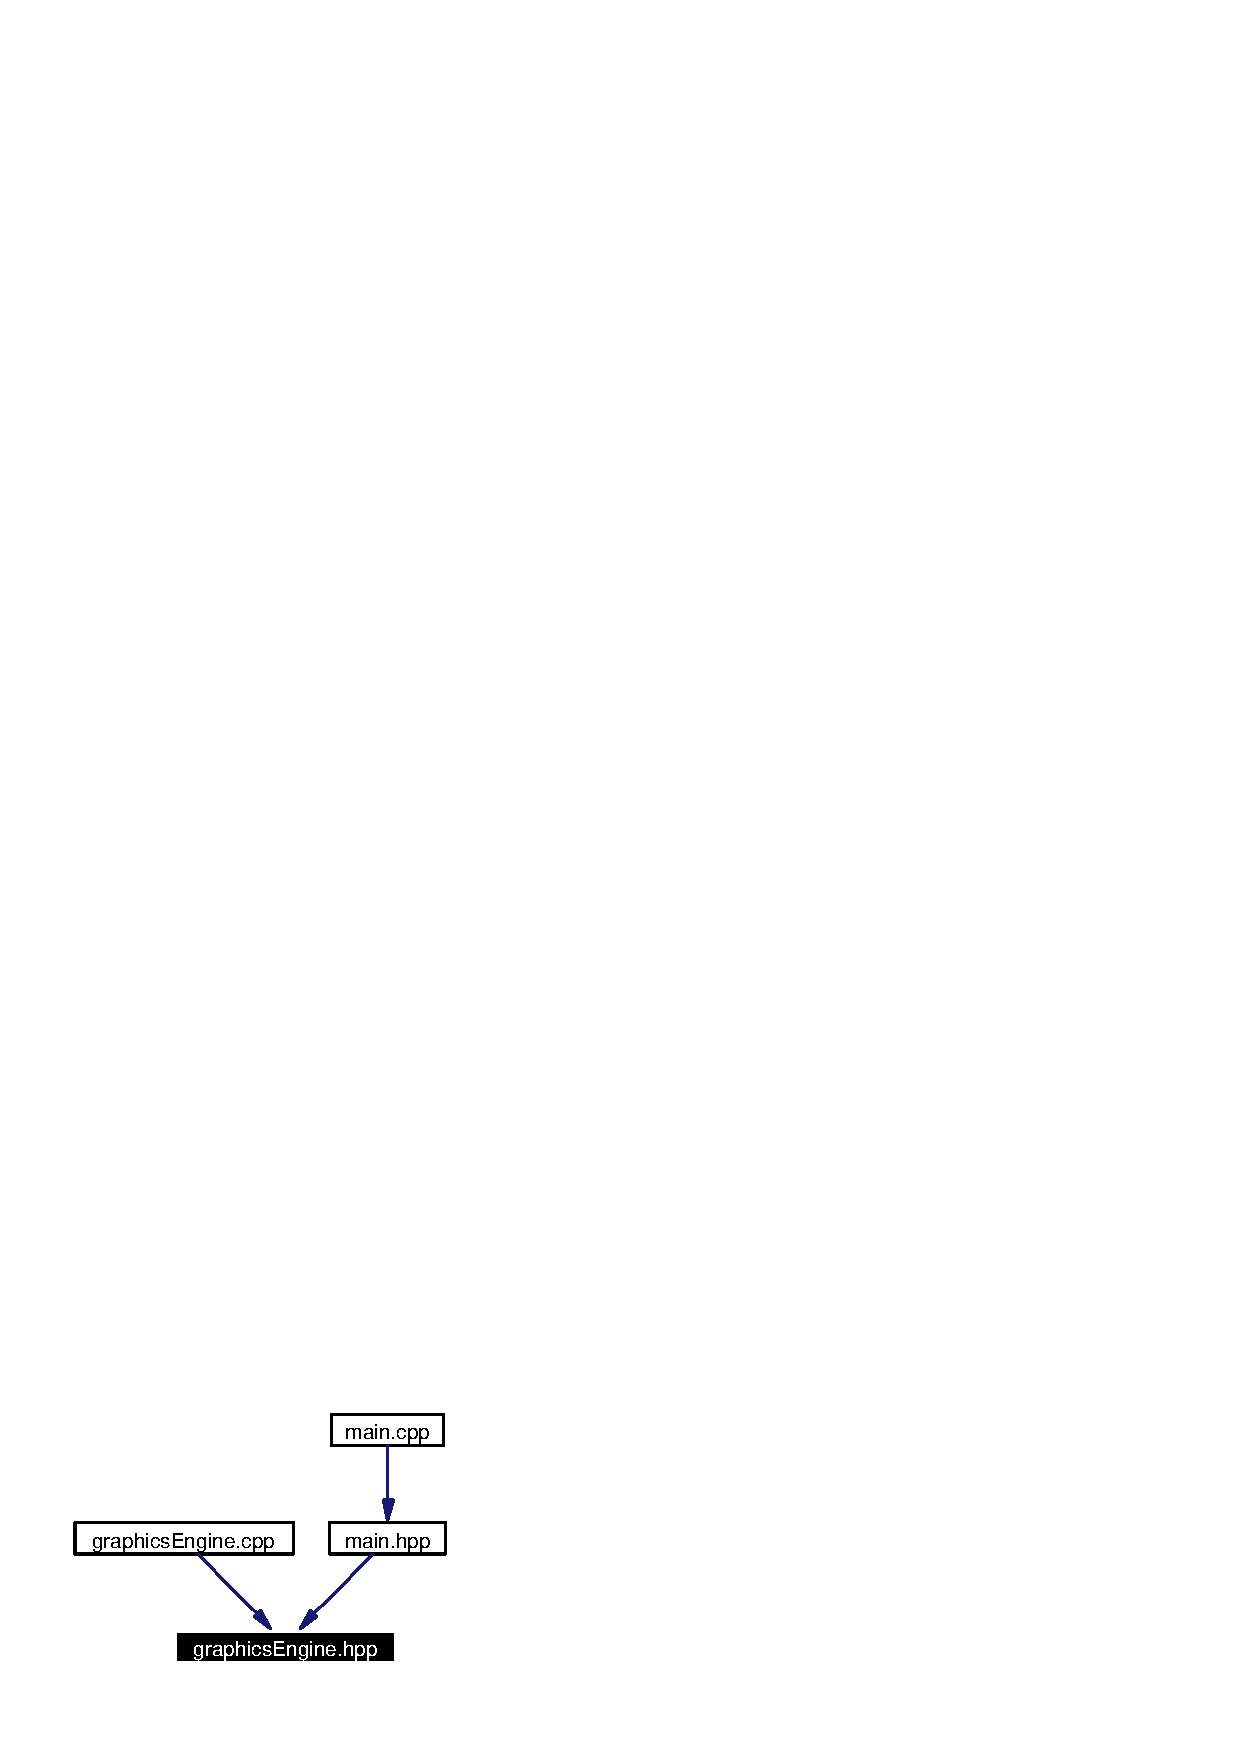
\includegraphics[width=107pt]{graphicsEngine_8hpp__dep__incl}
\end{center}
\end{figure}
\subsection*{Classes}
\begin{CompactItemize}
\item 
class {\bf Graphics\-Engine}
\end{CompactItemize}

\section{src/gui/gui\-Engine.cpp File Reference}
\label{guiEngine_8cpp}\index{src/gui/guiEngine.cpp@{src/gui/guiEngine.cpp}}
{\tt \#include \char`\"{}gui\-Engine.hpp\char`\"{}}\par


Include dependency graph for gui\-Engine.cpp:\begin{figure}[H]
\begin{center}
\leavevmode
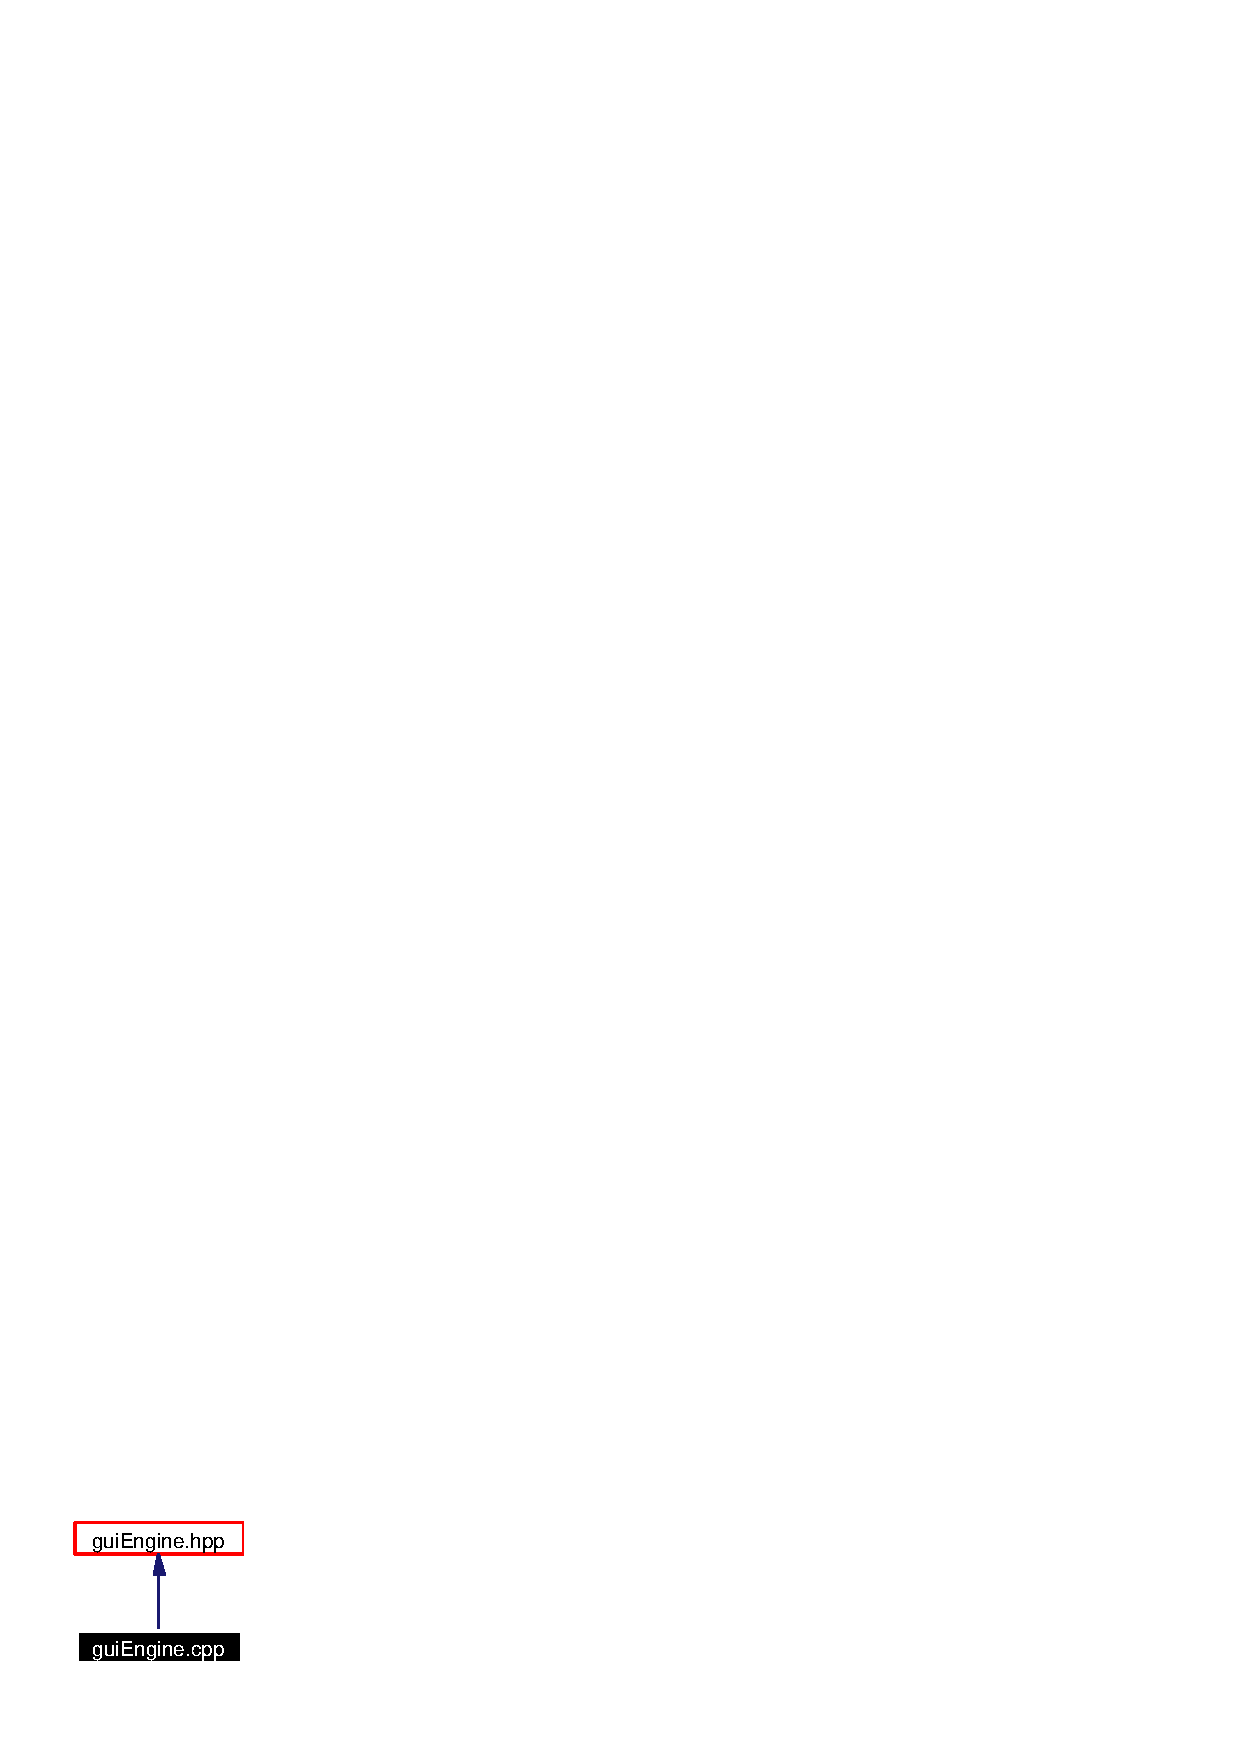
\includegraphics[width=58pt]{guiEngine_8cpp__incl}
\end{center}
\end{figure}
\subsection*{Functions}
\begin{CompactItemize}
\item 
{\bf PARAGUI\_\-CALLBACK} (options\-Menu\_\-handler)
\item 
{\bf PARAGUI\_\-CALLBACK} (go\-Back\_\-handler)
\item 
{\bf PARAGUI\_\-CALLBACK} (exit\_\-handler)
\item 
{\bf PARAGUI\_\-CALLBACK} (start\-Sim\_\-handler)
\item 
{\bf PARAGUI\_\-CALLBACK} (set\-Res800\_\-handler)
\item 
{\bf PARAGUI\_\-CALLBACK} (set\-Res640\_\-handler)
\end{CompactItemize}


\subsection{Function Documentation}
\index{guiEngine.cpp@{gui\-Engine.cpp}!PARAGUI_CALLBACK@{PARAGUI\_\-CALLBACK}}
\index{PARAGUI_CALLBACK@{PARAGUI\_\-CALLBACK}!guiEngine.cpp@{gui\-Engine.cpp}}
\subsubsection{\setlength{\rightskip}{0pt plus 5cm}PARAGUI\_\-CALLBACK (set\-Res640\_\-handler)}\label{guiEngine_8cpp_a5}


\index{guiEngine.cpp@{gui\-Engine.cpp}!PARAGUI_CALLBACK@{PARAGUI\_\-CALLBACK}}
\index{PARAGUI_CALLBACK@{PARAGUI\_\-CALLBACK}!guiEngine.cpp@{gui\-Engine.cpp}}
\subsubsection{\setlength{\rightskip}{0pt plus 5cm}PARAGUI\_\-CALLBACK (set\-Res800\_\-handler)}\label{guiEngine_8cpp_a4}


\index{guiEngine.cpp@{gui\-Engine.cpp}!PARAGUI_CALLBACK@{PARAGUI\_\-CALLBACK}}
\index{PARAGUI_CALLBACK@{PARAGUI\_\-CALLBACK}!guiEngine.cpp@{gui\-Engine.cpp}}
\subsubsection{\setlength{\rightskip}{0pt plus 5cm}PARAGUI\_\-CALLBACK (start\-Sim\_\-handler)}\label{guiEngine_8cpp_a3}


\index{guiEngine.cpp@{gui\-Engine.cpp}!PARAGUI_CALLBACK@{PARAGUI\_\-CALLBACK}}
\index{PARAGUI_CALLBACK@{PARAGUI\_\-CALLBACK}!guiEngine.cpp@{gui\-Engine.cpp}}
\subsubsection{\setlength{\rightskip}{0pt plus 5cm}PARAGUI\_\-CALLBACK (exit\_\-handler)}\label{guiEngine_8cpp_a2}


\index{guiEngine.cpp@{gui\-Engine.cpp}!PARAGUI_CALLBACK@{PARAGUI\_\-CALLBACK}}
\index{PARAGUI_CALLBACK@{PARAGUI\_\-CALLBACK}!guiEngine.cpp@{gui\-Engine.cpp}}
\subsubsection{\setlength{\rightskip}{0pt plus 5cm}PARAGUI\_\-CALLBACK (go\-Back\_\-handler)}\label{guiEngine_8cpp_a1}


\index{guiEngine.cpp@{gui\-Engine.cpp}!PARAGUI_CALLBACK@{PARAGUI\_\-CALLBACK}}
\index{PARAGUI_CALLBACK@{PARAGUI\_\-CALLBACK}!guiEngine.cpp@{gui\-Engine.cpp}}
\subsubsection{\setlength{\rightskip}{0pt plus 5cm}PARAGUI\_\-CALLBACK (options\-Menu\_\-handler)}\label{guiEngine_8cpp_a0}



\section{src/gui/gui\-Engine.hpp File Reference}
\label{guiEngine_8hpp}\index{src/gui/guiEngine.hpp@{src/gui/guiEngine.hpp}}
{\tt \#include \char`\"{}system.hpp\char`\"{}}\par
{\tt \#include \char`\"{}world.hpp\char`\"{}}\par
{\tt \#include \char`\"{}log\-Engine.hpp\char`\"{}}\par
{\tt \#include \char`\"{}SDL.h\char`\"{}}\par
{\tt \#include $<$paragui/paragui.h$>$}\par
{\tt \#include $<$paragui/pgapplication.h$>$}\par
{\tt \#include $<$paragui/pgwindow.h$>$}\par
{\tt \#include $<$paragui/pgbutton.h$>$}\par
{\tt \#include $<$paragui/pgwidgetlist.h$>$}\par
{\tt \#include $<$paragui/pglabel.h$>$}\par


Include dependency graph for gui\-Engine.hpp:\begin{figure}[H]
\begin{center}
\leavevmode
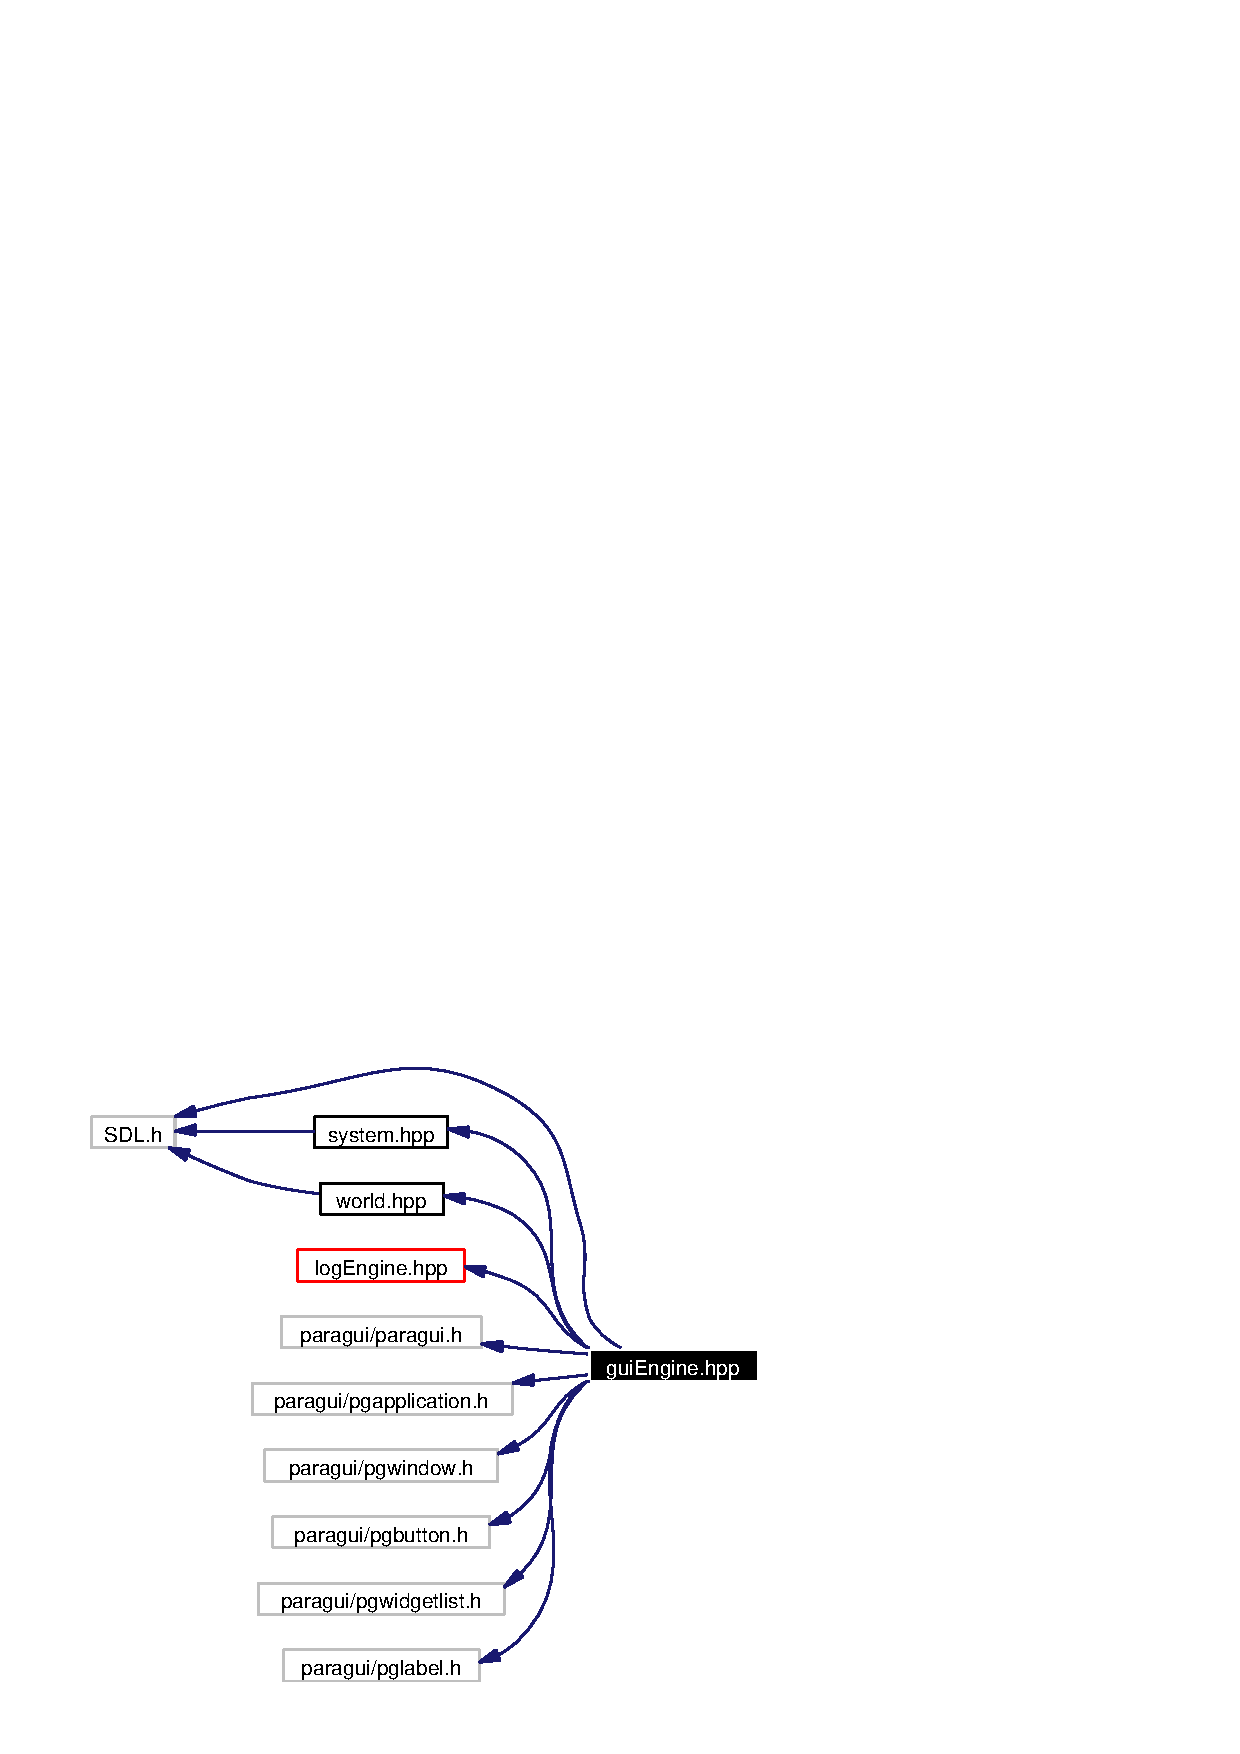
\includegraphics[width=186pt]{guiEngine_8hpp__incl}
\end{center}
\end{figure}


This graph shows which files directly or indirectly include this file:\begin{figure}[H]
\begin{center}
\leavevmode
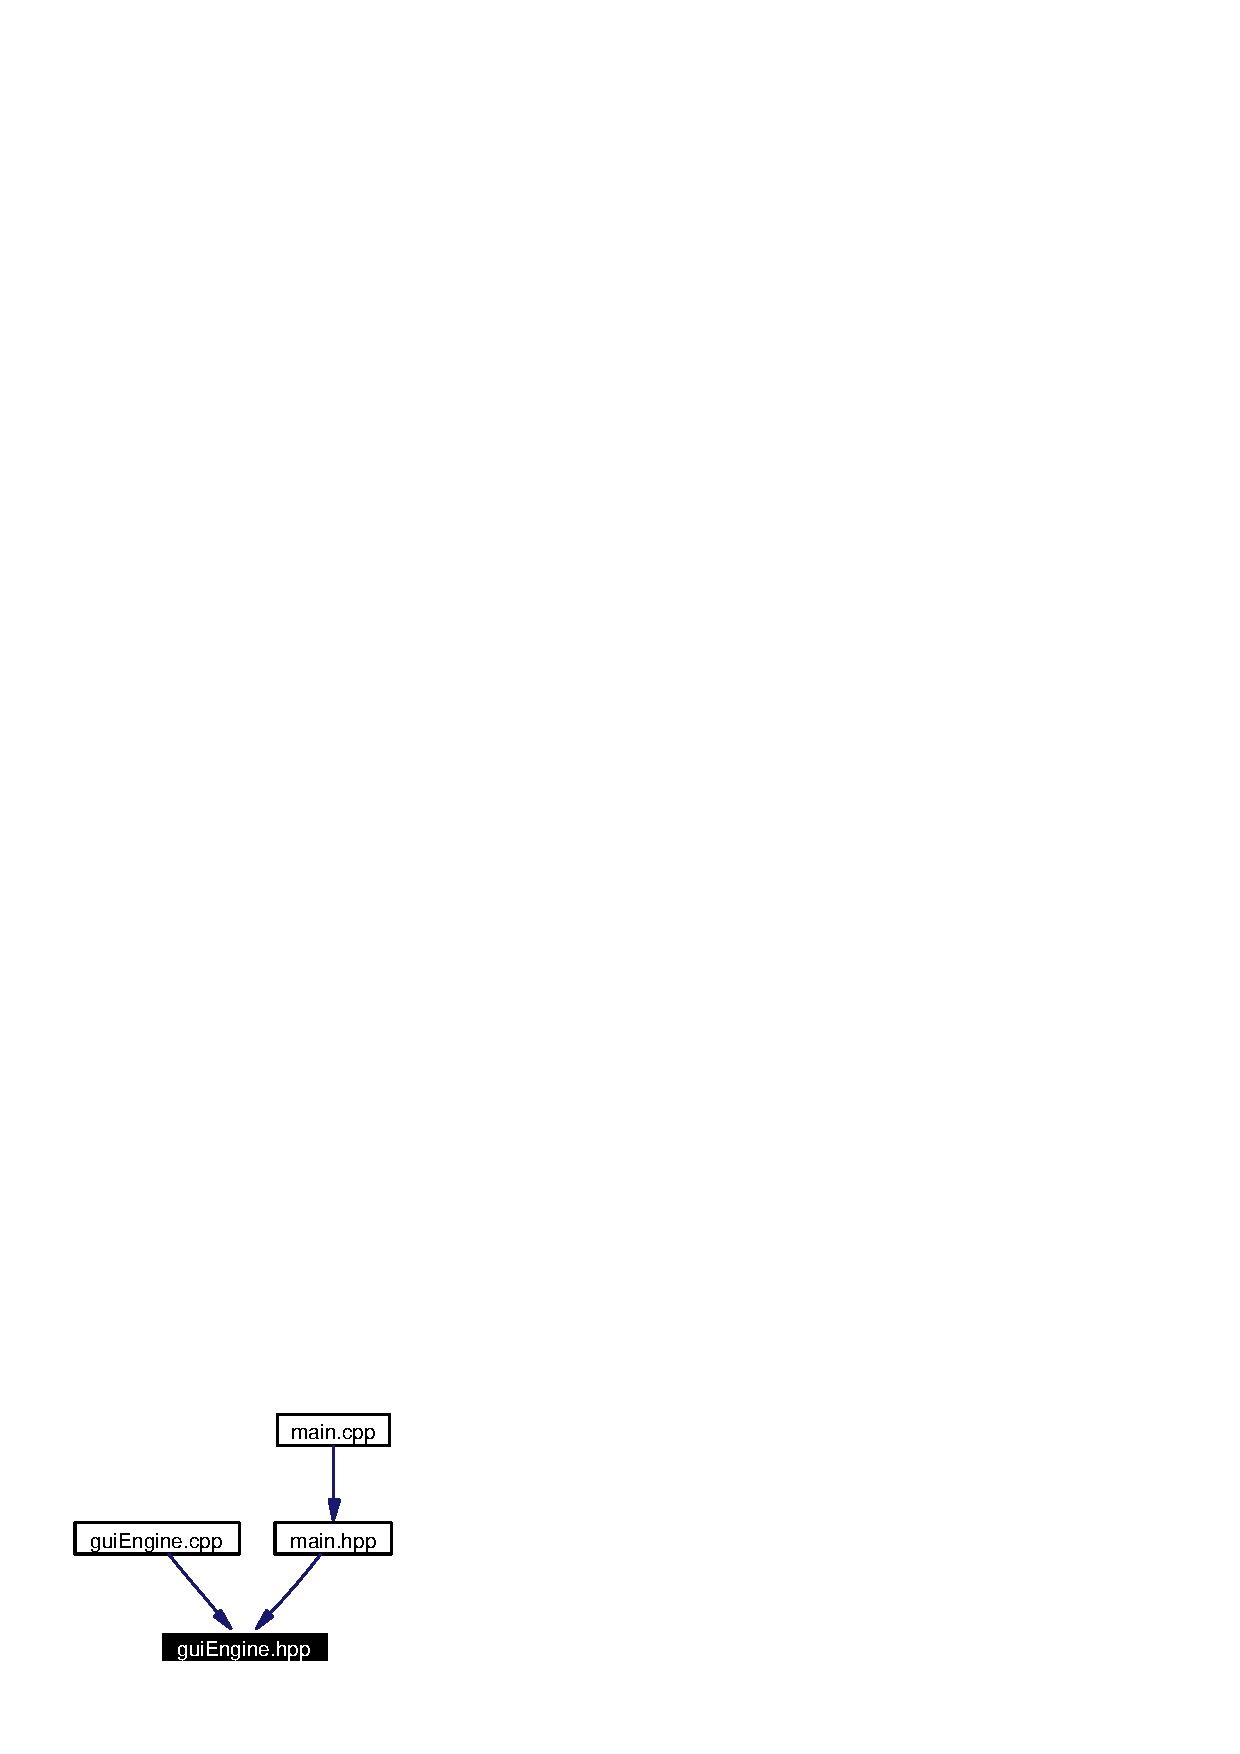
\includegraphics[width=94pt]{guiEngine_8hpp__dep__incl}
\end{center}
\end{figure}
\subsection*{Classes}
\begin{CompactItemize}
\item 
class {\bf Gui\-Engine}
\end{CompactItemize}

\section{src/gui/test\_\-paragui.cpp File Reference}
\label{test__paragui_8cpp}\index{src/gui/test_paragui.cpp@{src/gui/test\_\-paragui.cpp}}
{\tt \#include $<$paragui/paragui.h$>$}\par
{\tt \#include $<$paragui/pgapplication.h$>$}\par
{\tt \#include $<$paragui/pgbutton.h$>$}\par
{\tt \#include $<$paragui/pgwidgetlist.h$>$}\par
{\tt \#include $<$paragui/pglabel.h$>$}\par
{\tt \#include $<$paragui/pgwindow.h$>$}\par
{\tt \#include $<$paragui/pgmaskedit.h$>$}\par
{\tt \#include $<$paragui/pgscrollbar.h$>$}\par
{\tt \#include $<$paragui/pgprogressbar.h$>$}\par
{\tt \#include $<$paragui/pgradiobutton.h$>$}\par
{\tt \#include $<$paragui/pgthemewidget.h$>$}\par
{\tt \#include $<$paragui/pgcheckbutton.h$>$}\par
{\tt \#include $<$paragui/pgslider.h$>$}\par
{\tt \#include $<$paragui/pglistbox.h$>$}\par
{\tt \#include $<$paragui/pgcolumnitem.h$>$}\par
{\tt \#include $<$paragui/pgdropdown.h$>$}\par
{\tt \#include $<$paragui/pgeventobject.h$>$}\par
{\tt \#include $<$paragui/pgpopupmenu.h$>$}\par
{\tt \#include $<$paragui/pgspinnerbox.h$>$}\par
{\tt \#include $<$paragui/pglog.h$>$}\par
{\tt \#include $<$paragui/pgmenubar.h$>$}\par


Include dependency graph for test\_\-paragui.cpp:\begin{figure}[H]
\begin{center}
\leavevmode
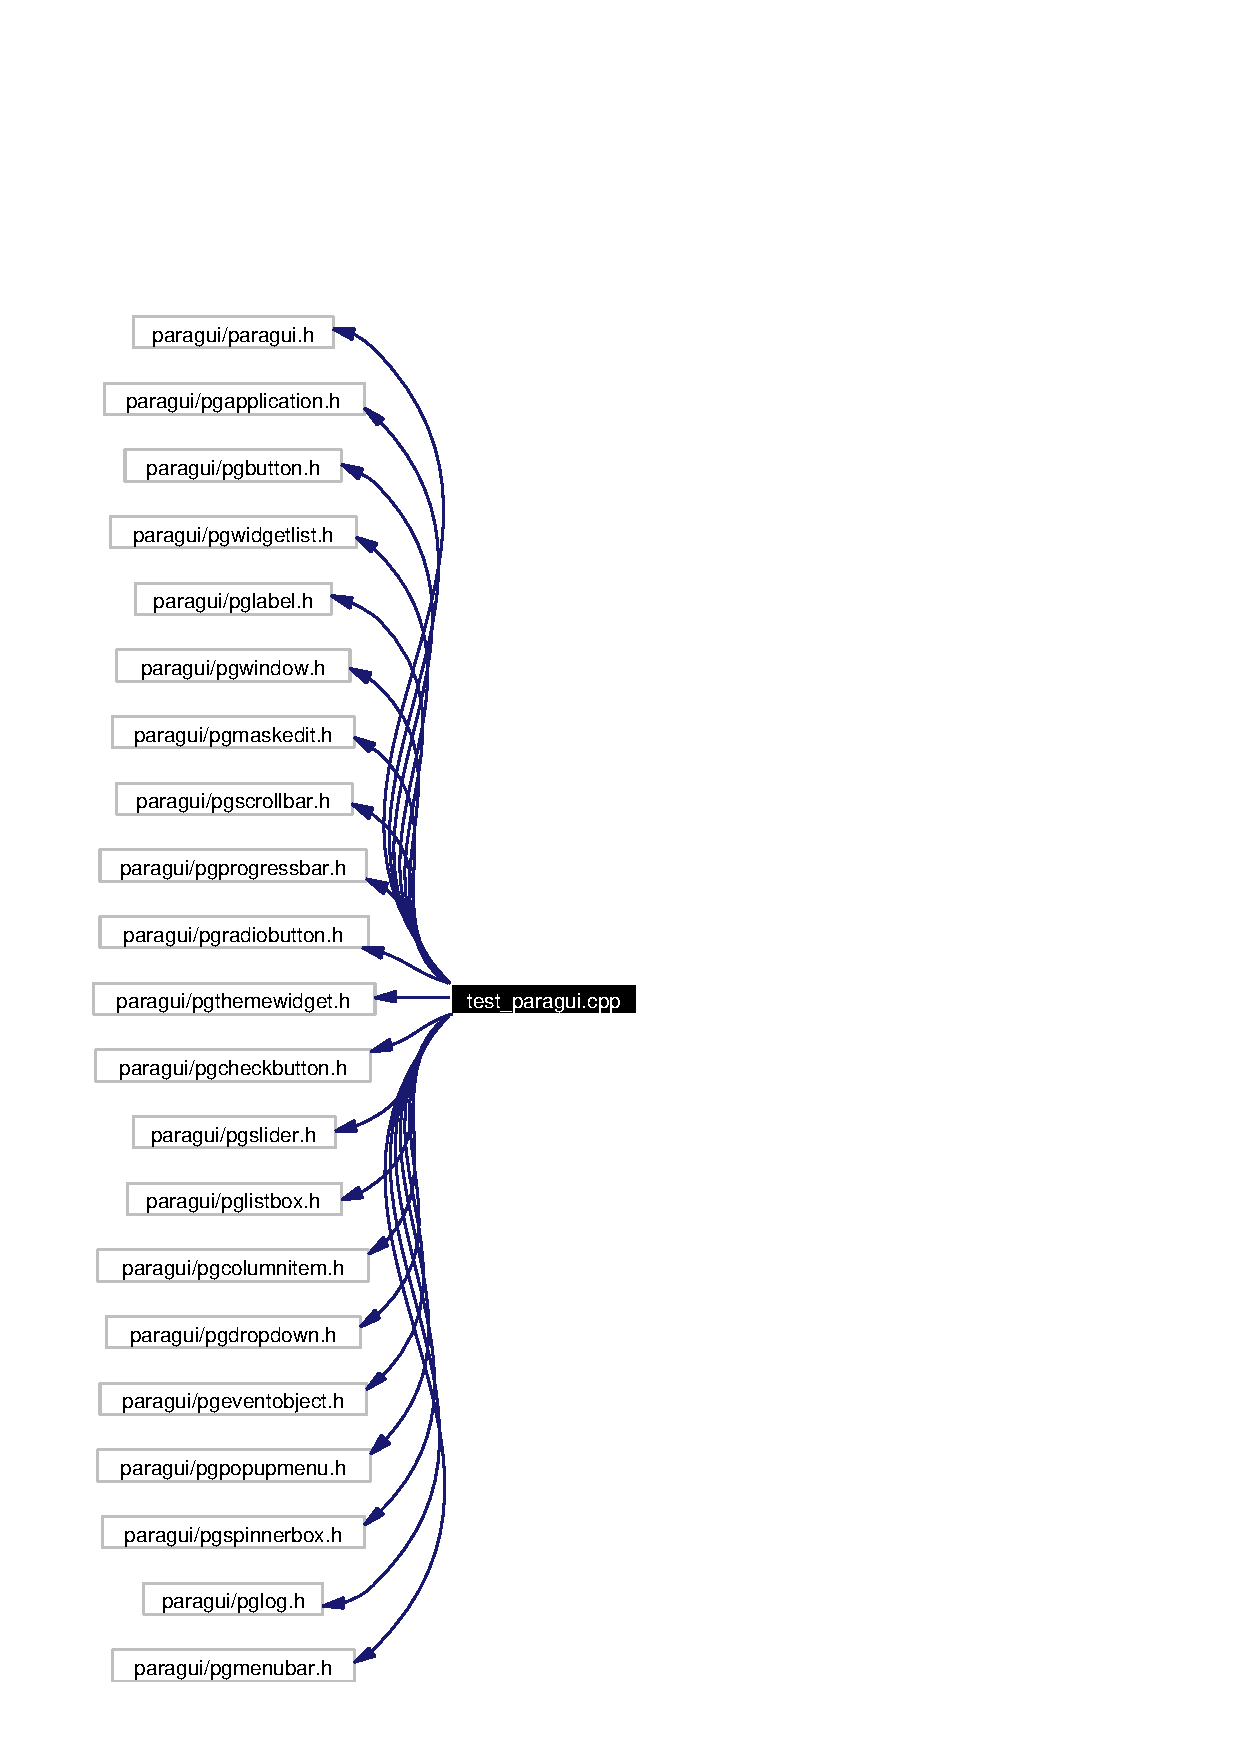
\includegraphics[width=157pt]{test__paragui_8cpp__incl}
\end{center}
\end{figure}
\subsection*{Classes}
\begin{CompactItemize}
\item 
class {\bf Test\-Window}
\end{CompactItemize}
\subsection*{Defines}
\begin{CompactItemize}
\item 
\#define {\bf Set\-Connection}(MSG\_\-TYPE, obj\-Dest, obj\-Func)\ Set\-Event\-Object(MSG\_\-TYPE, obj\-Dest, (MSG\_\-CALLBACK\_\-OBJ)\&obj\-Func)
\item 
\#define {\bf RESX}\ 800
\item 
\#define {\bf RESY}\ 600
\end{CompactItemize}
\subsection*{Functions}
\begin{CompactItemize}
\item 
void {\bf Splash} ()
\end{CompactItemize}


\subsection{Define Documentation}
\index{test_paragui.cpp@{test\_\-paragui.cpp}!RESX@{RESX}}
\index{RESX@{RESX}!test_paragui.cpp@{test\_\-paragui.cpp}}
\subsubsection{\setlength{\rightskip}{0pt plus 5cm}\#define RESX\ 800}\label{test__paragui_8cpp_a1}


\index{test_paragui.cpp@{test\_\-paragui.cpp}!RESY@{RESY}}
\index{RESY@{RESY}!test_paragui.cpp@{test\_\-paragui.cpp}}
\subsubsection{\setlength{\rightskip}{0pt plus 5cm}\#define RESY\ 600}\label{test__paragui_8cpp_a2}


\index{test_paragui.cpp@{test\_\-paragui.cpp}!SetConnection@{SetConnection}}
\index{SetConnection@{SetConnection}!test_paragui.cpp@{test\_\-paragui.cpp}}
\subsubsection{\setlength{\rightskip}{0pt plus 5cm}\#define Set\-Connection(MSG\_\-TYPE, obj\-Dest, obj\-Func)\ Set\-Event\-Object(MSG\_\-TYPE, obj\-Dest, (MSG\_\-CALLBACK\_\-OBJ)\&obj\-Func)}\label{test__paragui_8cpp_a0}




\subsection{Function Documentation}
\index{test_paragui.cpp@{test\_\-paragui.cpp}!Splash@{Splash}}
\index{Splash@{Splash}!test_paragui.cpp@{test\_\-paragui.cpp}}
\subsubsection{\setlength{\rightskip}{0pt plus 5cm}void Splash ()}\label{test__paragui_8cpp_a3}



\section{src/input/input\-Engine.cpp File Reference}
\label{inputEngine_8cpp}\index{src/input/inputEngine.cpp@{src/input/inputEngine.cpp}}
{\tt \#include \char`\"{}input\-Engine.hpp\char`\"{}}\par


Include dependency graph for input\-Engine.cpp:\begin{figure}[H]
\begin{center}
\leavevmode
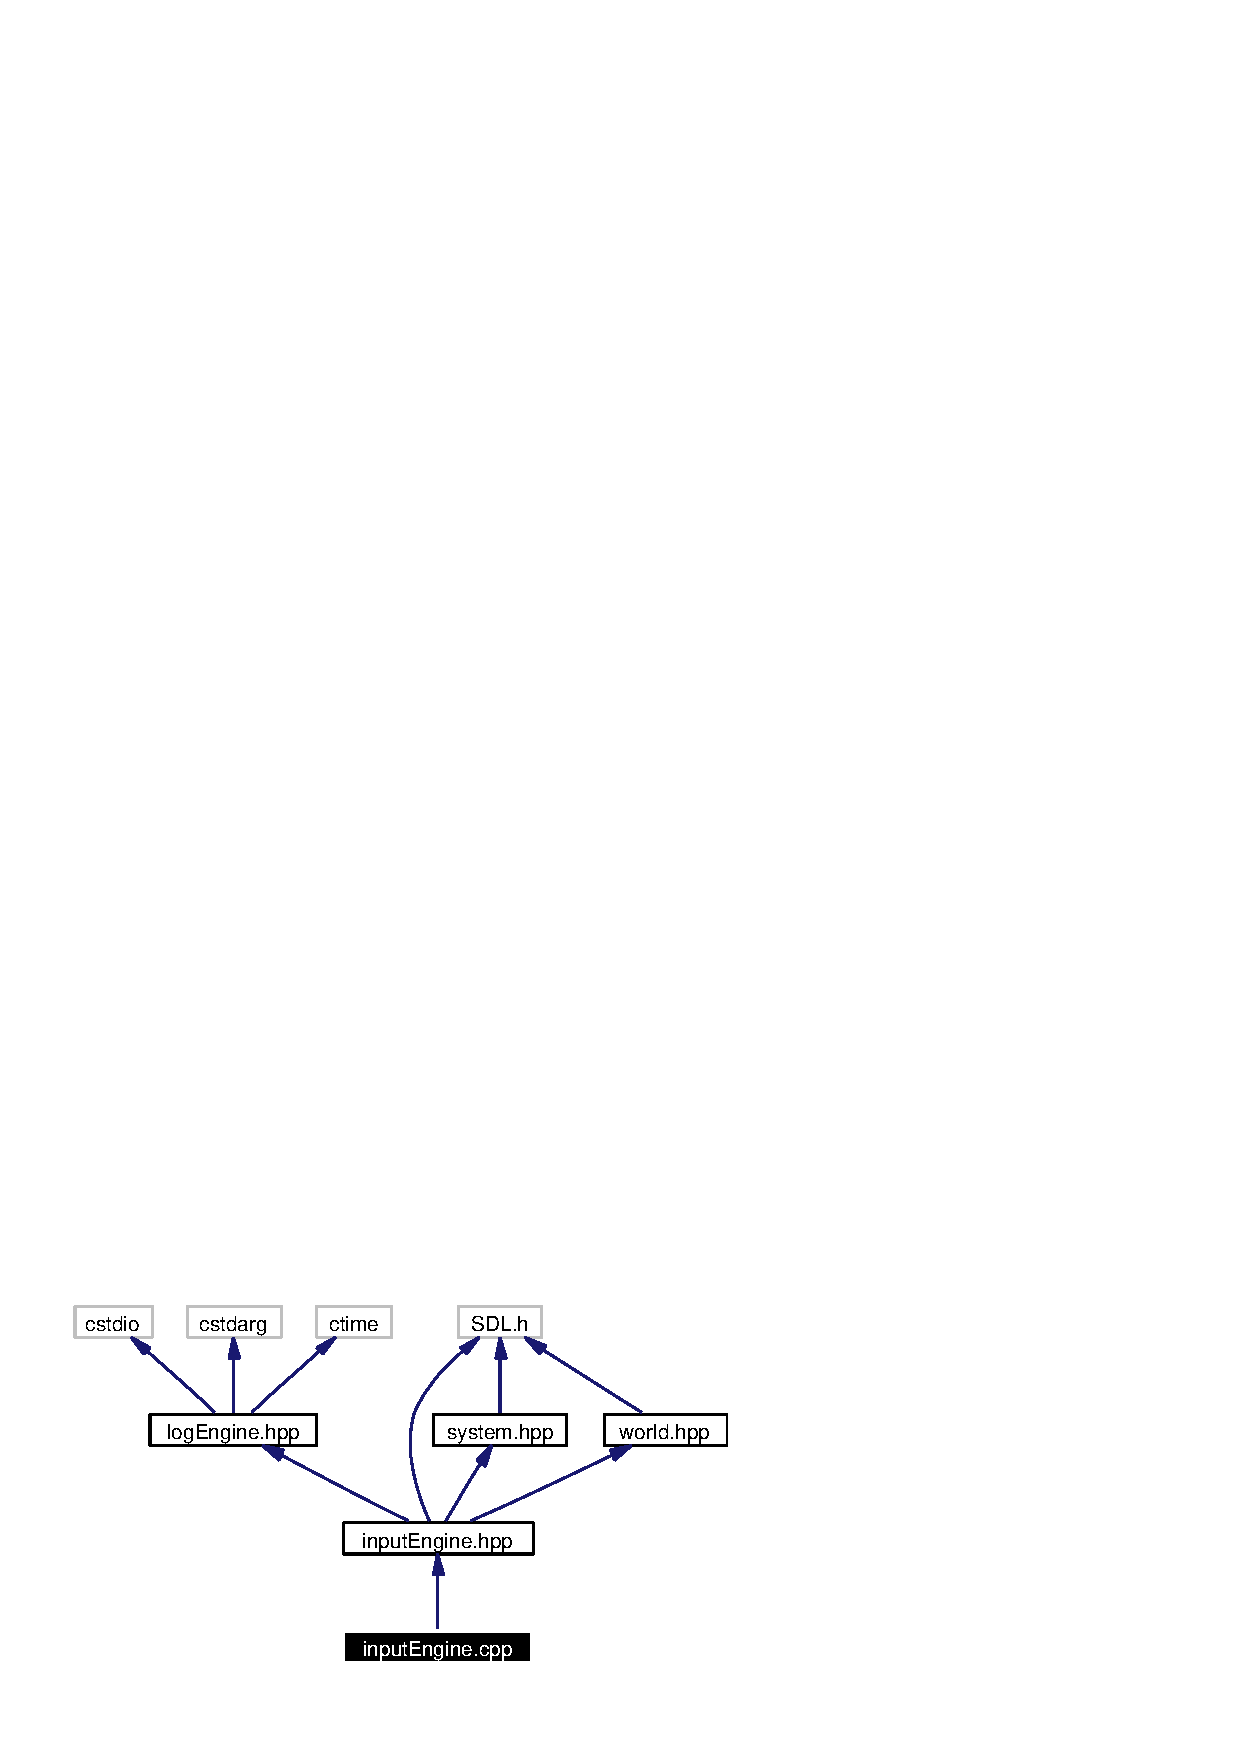
\includegraphics[width=174pt]{inputEngine_8cpp__incl}
\end{center}
\end{figure}

\section{src/input/input\-Engine.hpp File Reference}
\label{inputEngine_8hpp}\index{src/input/inputEngine.hpp@{src/input/inputEngine.hpp}}
{\tt \#include \char`\"{}log\-Engine.hpp\char`\"{}}\par
{\tt \#include \char`\"{}SDL.h\char`\"{}}\par
{\tt \#include \char`\"{}system.hpp\char`\"{}}\par
{\tt \#include \char`\"{}world.hpp\char`\"{}}\par


Include dependency graph for input\-Engine.hpp:\begin{figure}[H]
\begin{center}
\leavevmode
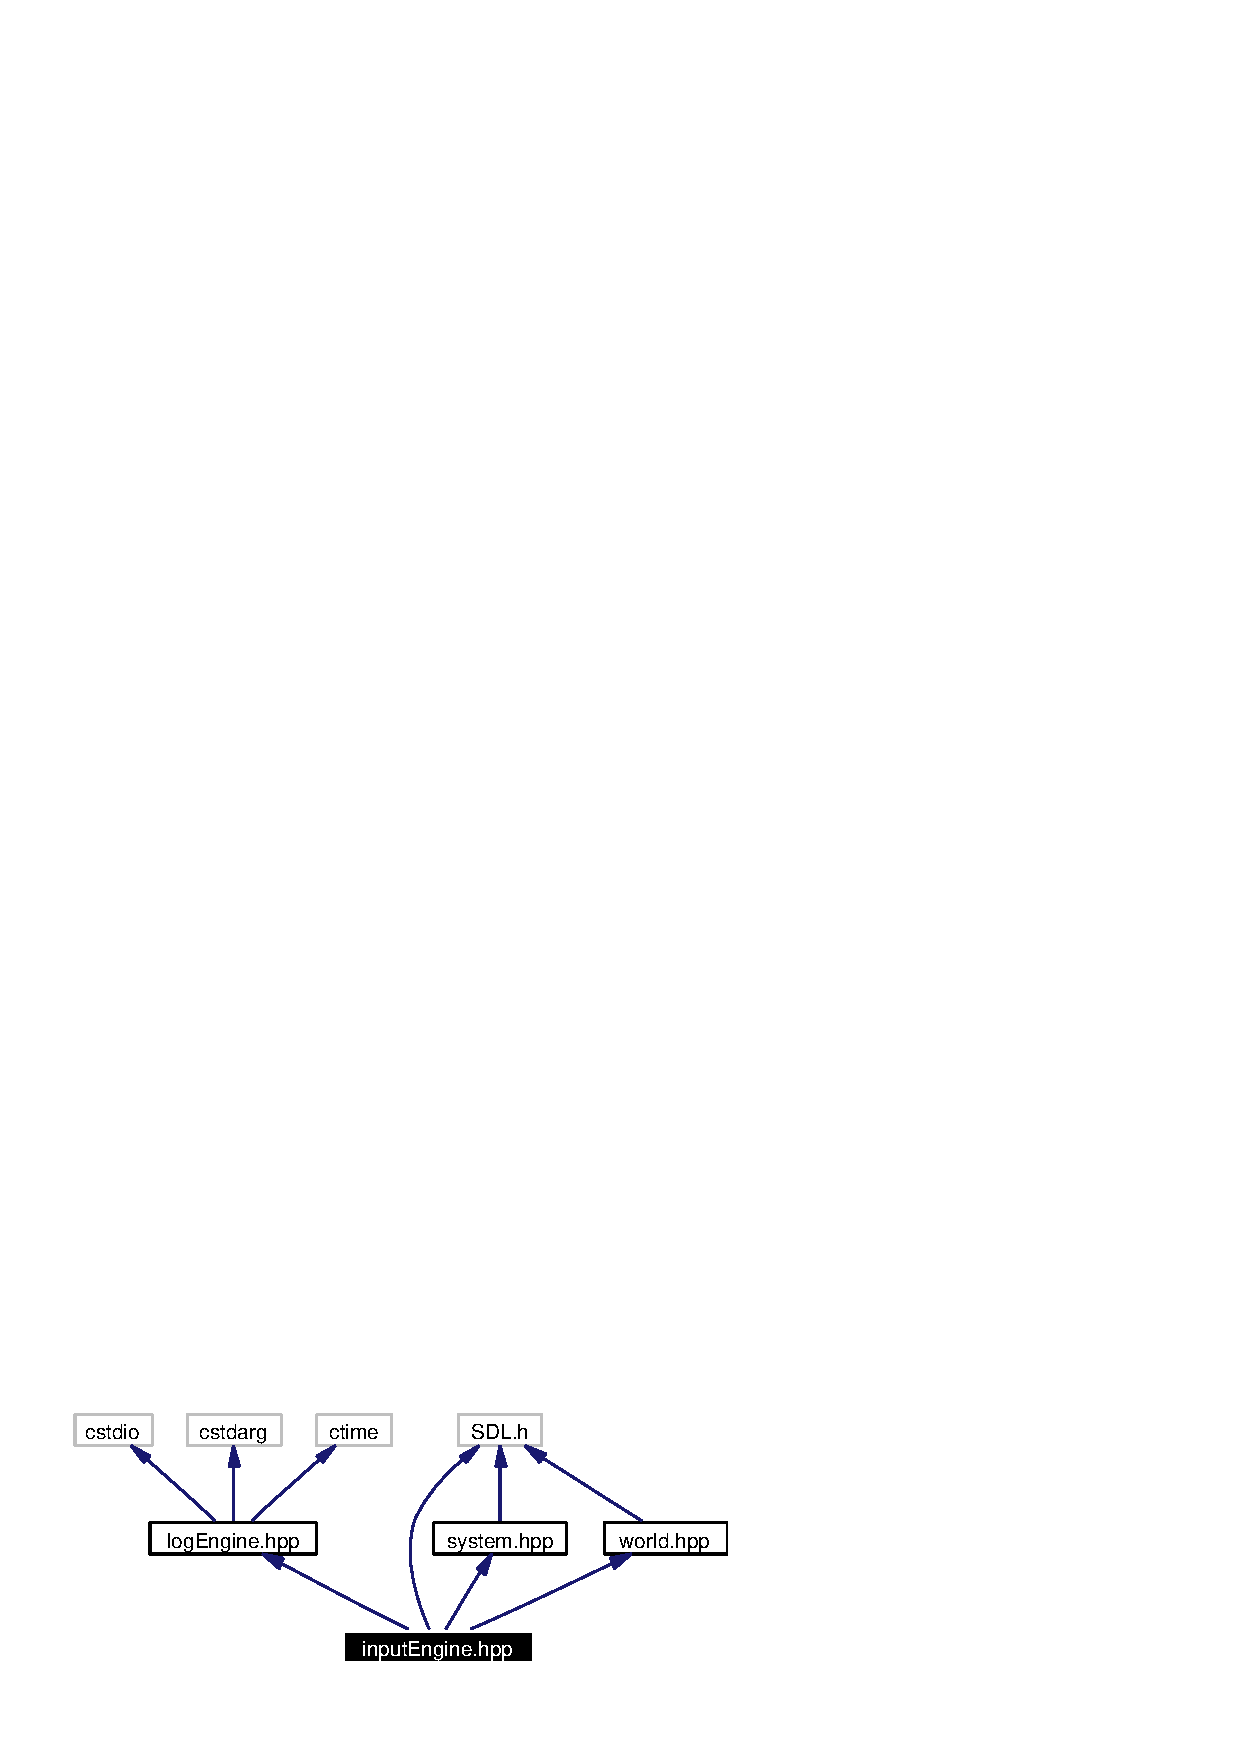
\includegraphics[width=174pt]{inputEngine_8hpp__incl}
\end{center}
\end{figure}


This graph shows which files directly or indirectly include this file:\begin{figure}[H]
\begin{center}
\leavevmode
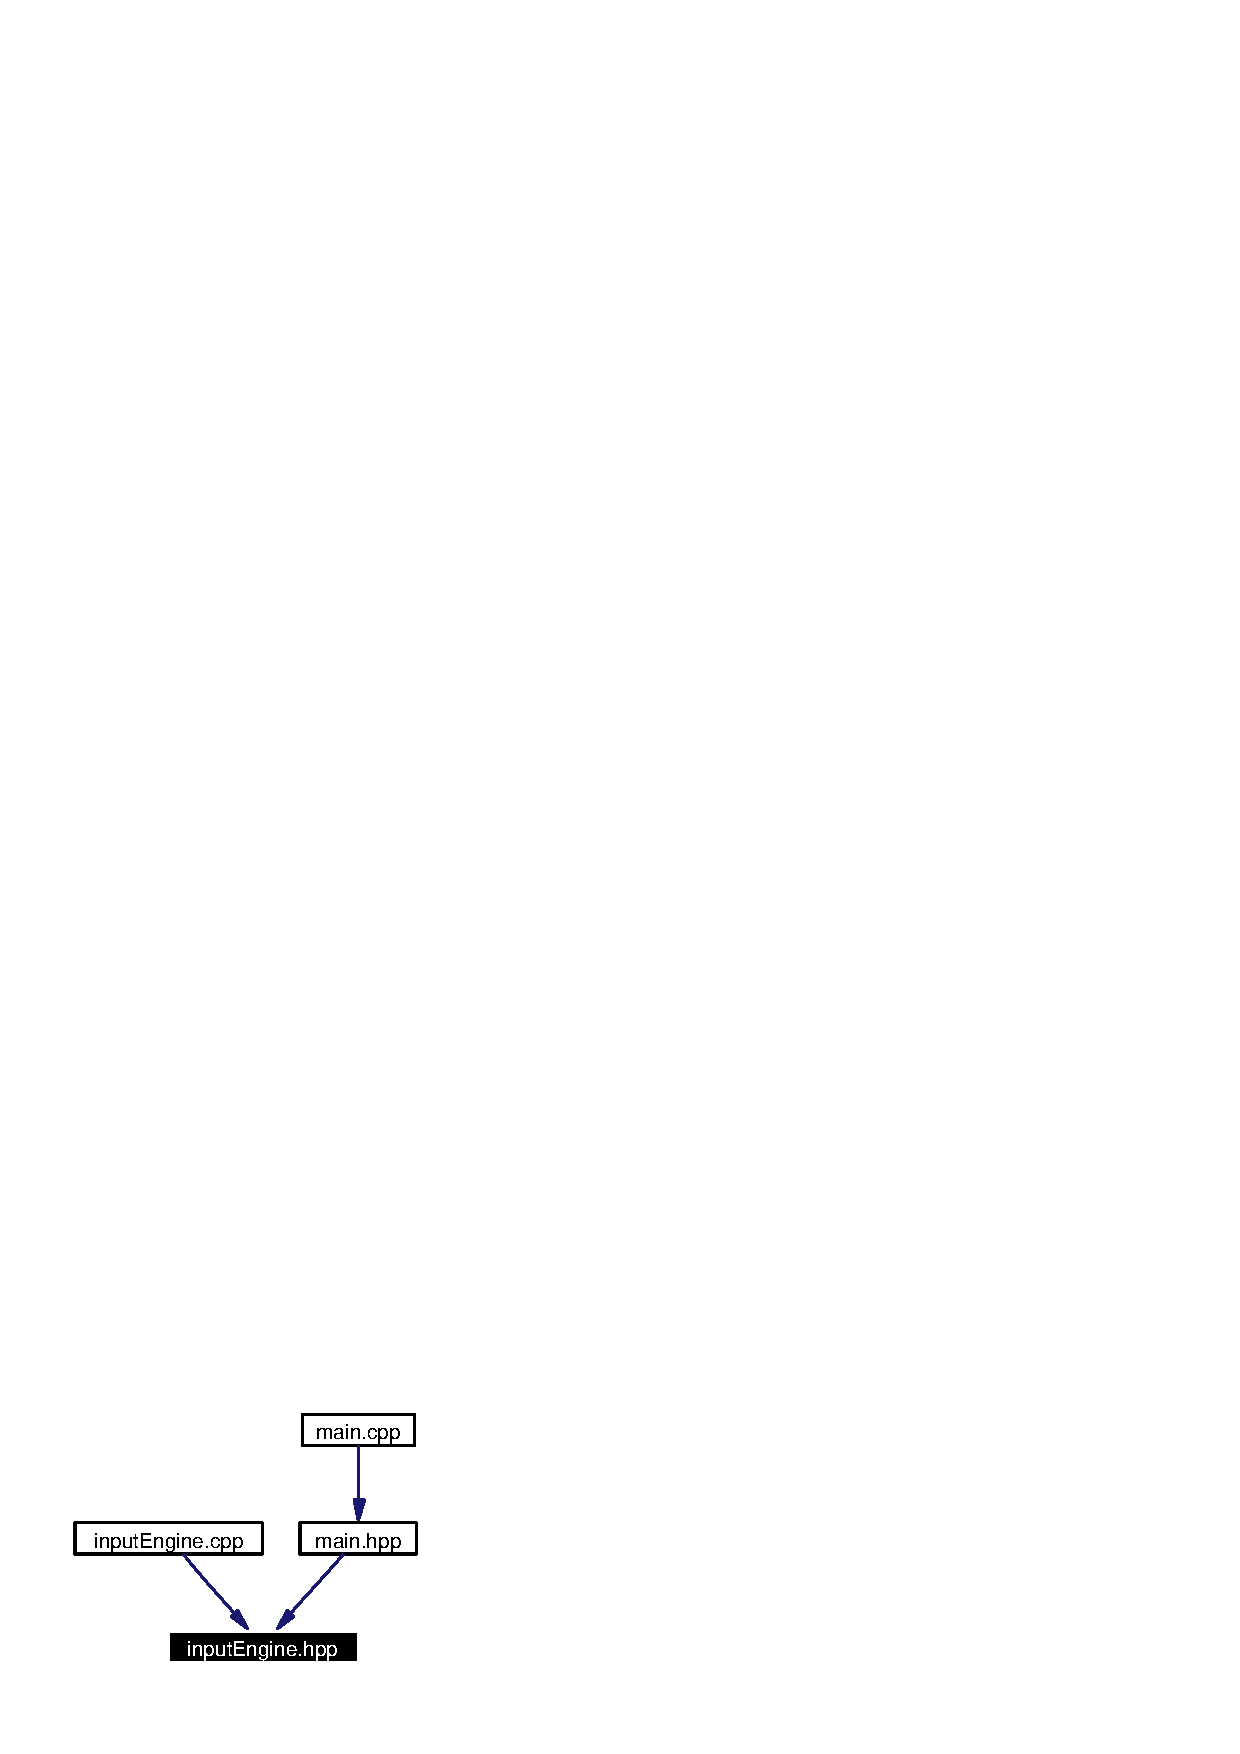
\includegraphics[width=100pt]{inputEngine_8hpp__dep__incl}
\end{center}
\end{figure}
\subsection*{Classes}
\begin{CompactItemize}
\item 
class {\bf Input\-Engine}
\end{CompactItemize}

\section{src/log/log\-Engine.cpp File Reference}
\label{logEngine_8cpp}\index{src/log/logEngine.cpp@{src/log/logEngine.cpp}}
{\tt \#include \char`\"{}log\-Engine.hpp\char`\"{}}\par


Include dependency graph for log\-Engine.cpp:\begin{figure}[H]
\begin{center}
\leavevmode
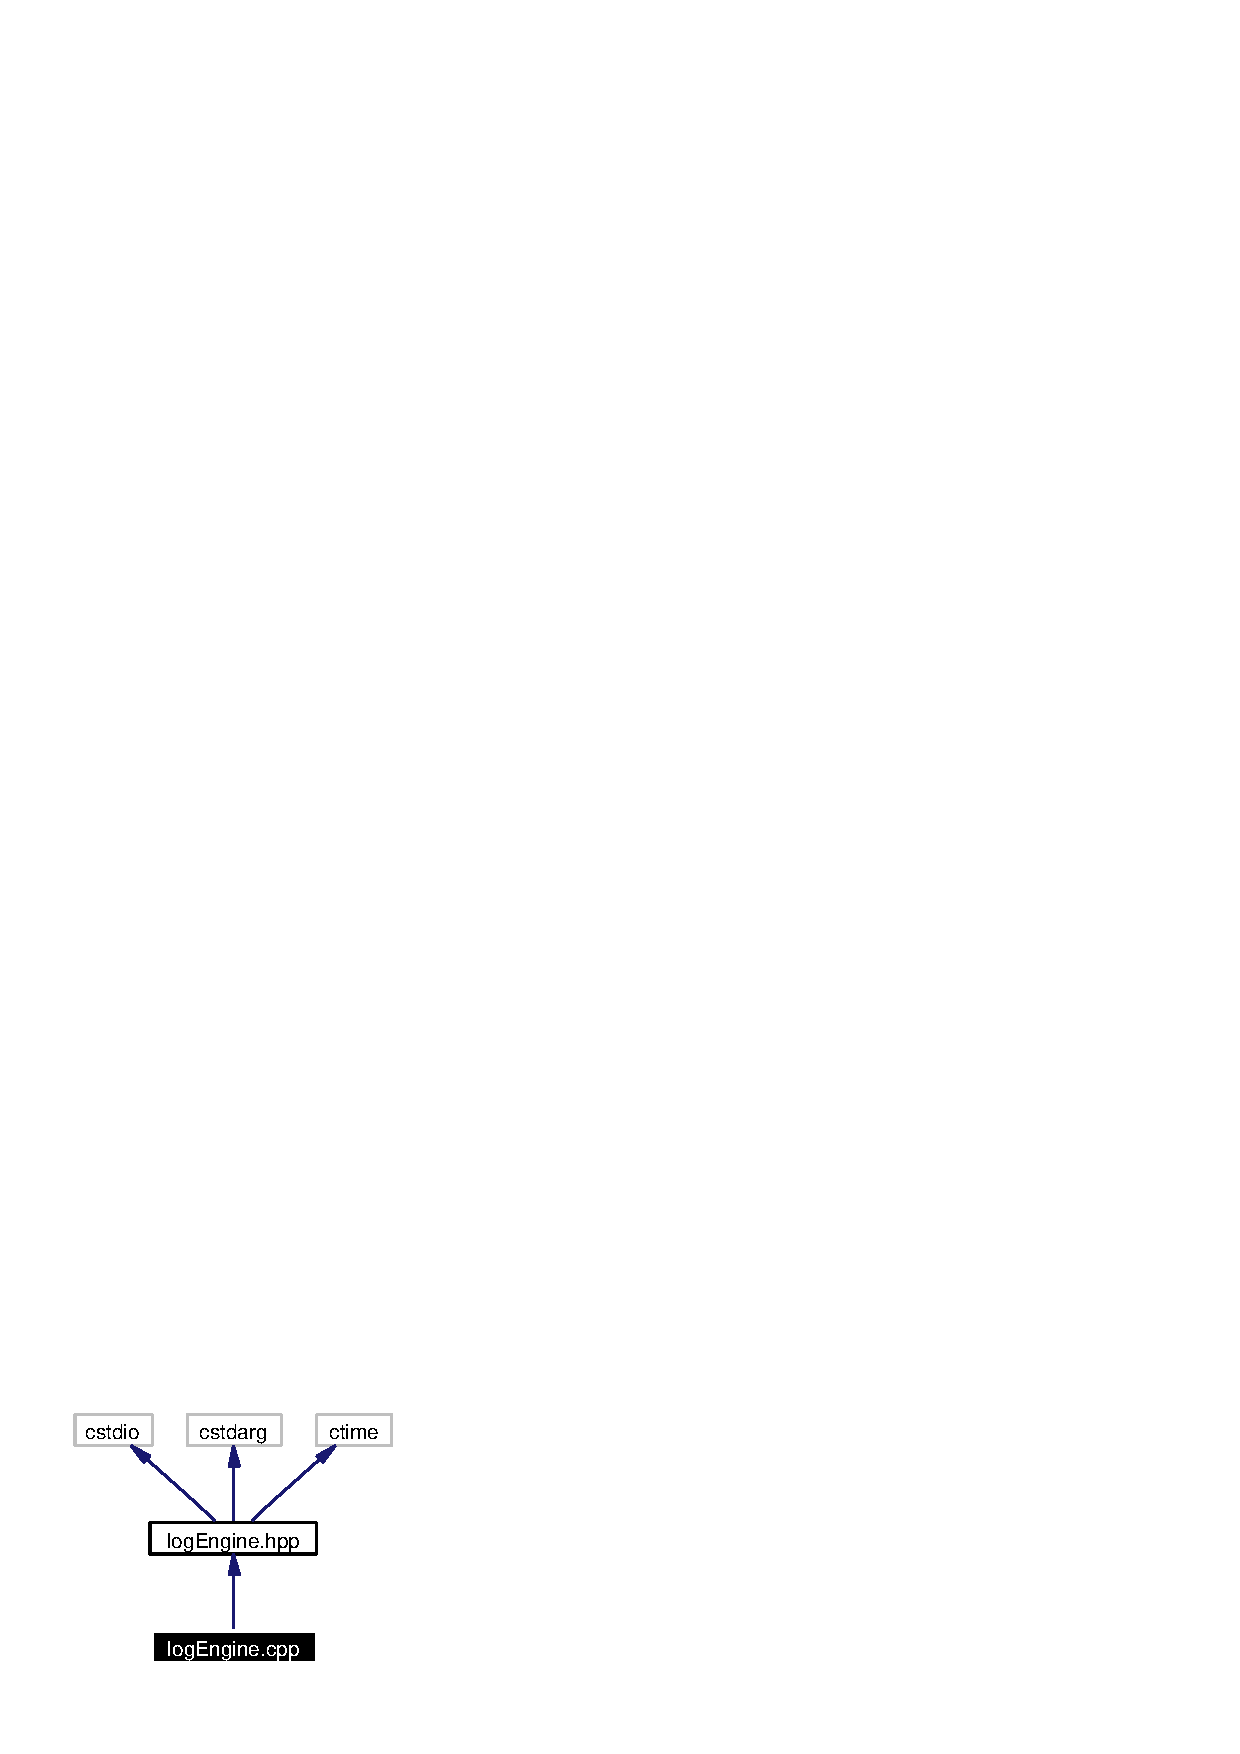
\includegraphics[width=94pt]{logEngine_8cpp__incl}
\end{center}
\end{figure}

\section{src/log/log\-Engine.hpp File Reference}
\label{logEngine_8hpp}\index{src/log/logEngine.hpp@{src/log/logEngine.hpp}}
{\tt \#include $<$cstdio$>$}\par
{\tt \#include $<$cstdarg$>$}\par
{\tt \#include $<$ctime$>$}\par


Include dependency graph for log\-Engine.hpp:\begin{figure}[H]
\begin{center}
\leavevmode
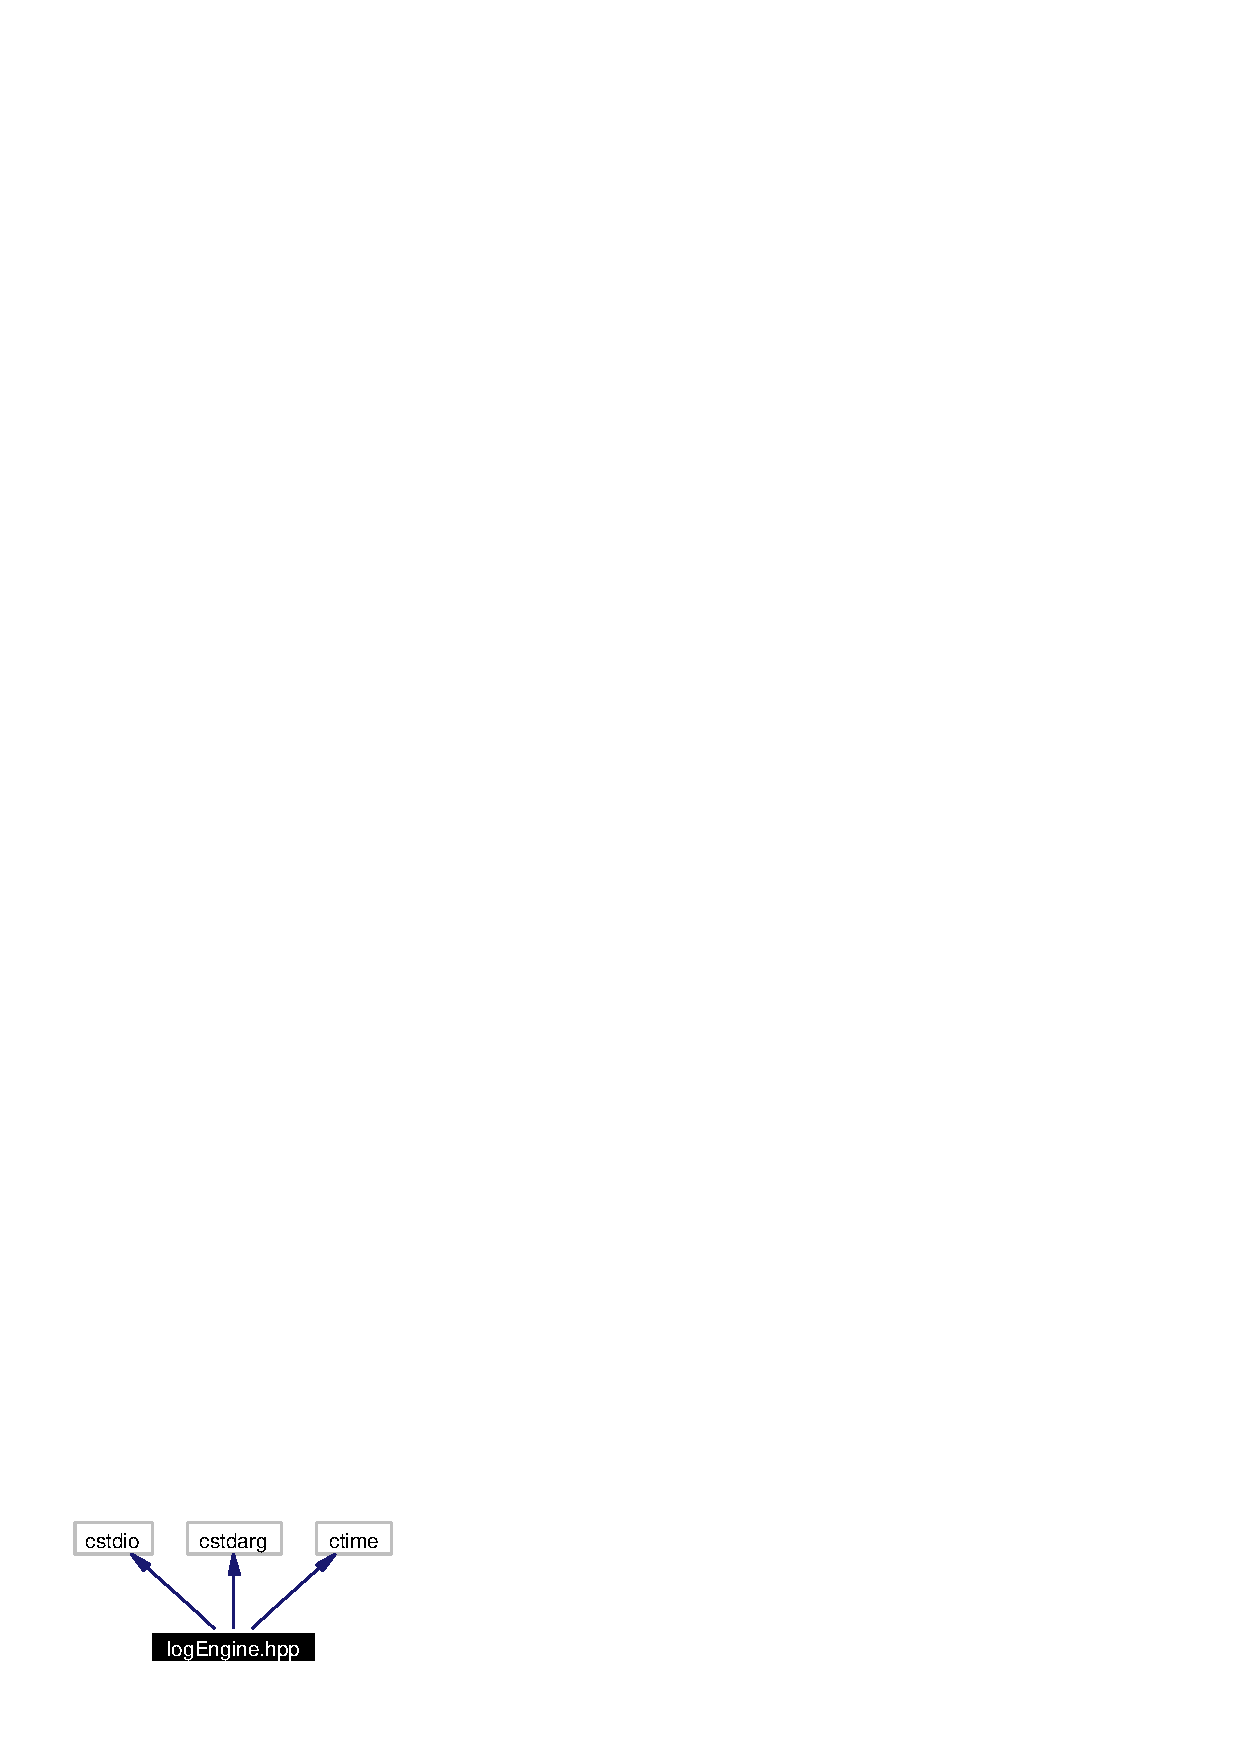
\includegraphics[width=94pt]{logEngine_8hpp__incl}
\end{center}
\end{figure}


This graph shows which files directly or indirectly include this file:\begin{figure}[H]
\begin{center}
\leavevmode
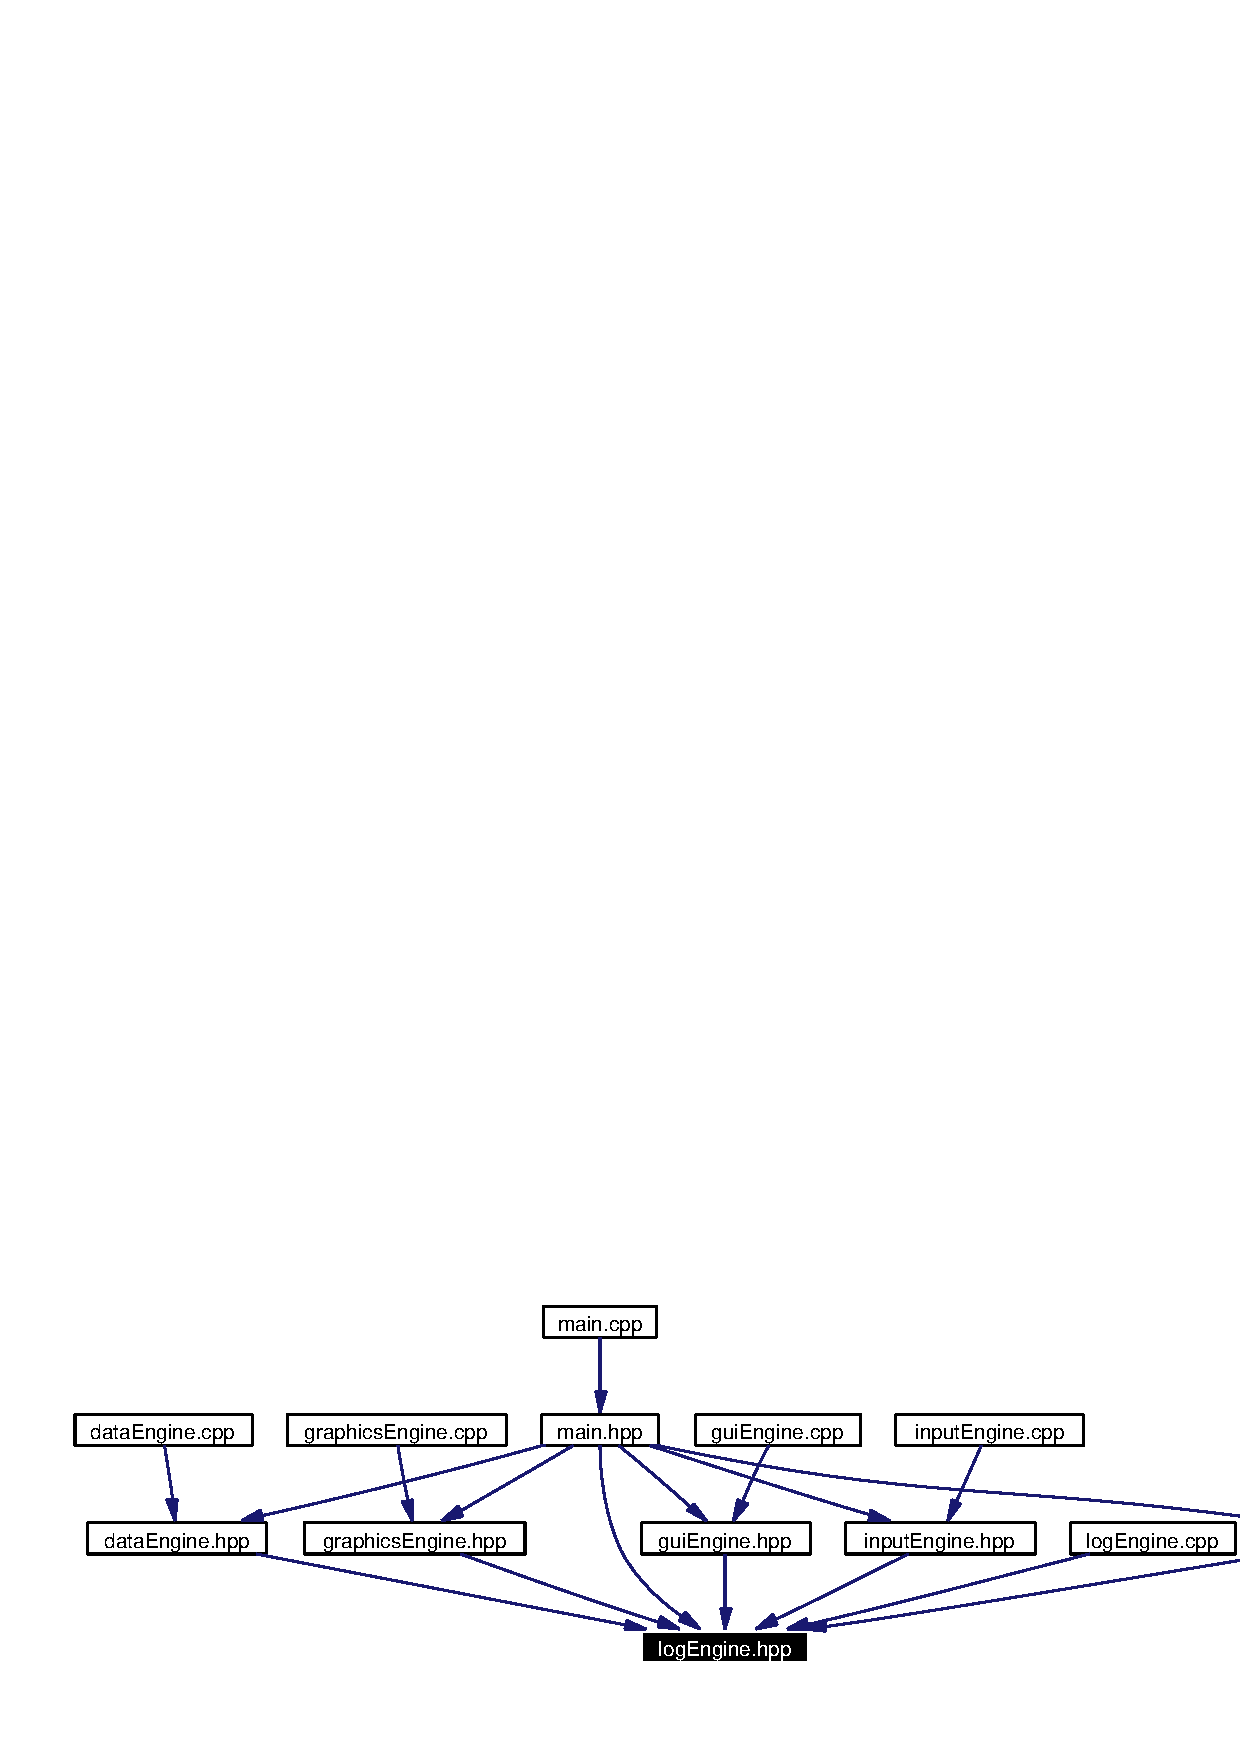
\includegraphics[width=355pt]{logEngine_8hpp__dep__incl}
\end{center}
\end{figure}
\subsection*{Classes}
\begin{CompactItemize}
\item 
class {\bf Log\-Engine}
\end{CompactItemize}
\subsection*{Enumerations}
\begin{CompactItemize}
\item 
enum {\bf LOG\_\-LEVEL} \{ \par
{\bf LOG\_\-ERROR} =  0, 
{\bf LOG\_\-WARNING} =  1, 
{\bf LOG\_\-INFO} =  2, 
{\bf LOG\_\-VERBOSE} =  3, 
\par
{\bf LOG\_\-TRACE} =  4
 \}
\end{CompactItemize}


\subsection{Enumeration Type Documentation}
\index{logEngine.hpp@{log\-Engine.hpp}!LOG_LEVEL@{LOG\_\-LEVEL}}
\index{LOG_LEVEL@{LOG\_\-LEVEL}!logEngine.hpp@{log\-Engine.hpp}}
\subsubsection{\setlength{\rightskip}{0pt plus 5cm}enum {\bf LOG\_\-LEVEL}}\label{logEngine_8hpp_a5}


\begin{Desc}
\item[Enumeration values: ]\par
\begin{description}
\index{LOG_ERROR@{LOG\_\-ERROR}!logEngine.hpp@{logEngine.hpp}}\index{logEngine.hpp@{logEngine.hpp}!LOG_ERROR@{LOG\_\-ERROR}}\item[{\em 
LOG\_\-ERROR\label{logEngine_8hpp_a5a0}
}]\index{LOG_WARNING@{LOG\_\-WARNING}!logEngine.hpp@{logEngine.hpp}}\index{logEngine.hpp@{logEngine.hpp}!LOG_WARNING@{LOG\_\-WARNING}}\item[{\em 
LOG\_\-WARNING\label{logEngine_8hpp_a5a1}
}]\index{LOG_INFO@{LOG\_\-INFO}!logEngine.hpp@{logEngine.hpp}}\index{logEngine.hpp@{logEngine.hpp}!LOG_INFO@{LOG\_\-INFO}}\item[{\em 
LOG\_\-INFO\label{logEngine_8hpp_a5a2}
}]\index{LOG_VERBOSE@{LOG\_\-VERBOSE}!logEngine.hpp@{logEngine.hpp}}\index{logEngine.hpp@{logEngine.hpp}!LOG_VERBOSE@{LOG\_\-VERBOSE}}\item[{\em 
LOG\_\-VERBOSE\label{logEngine_8hpp_a5a3}
}]\index{LOG_TRACE@{LOG\_\-TRACE}!logEngine.hpp@{logEngine.hpp}}\index{logEngine.hpp@{logEngine.hpp}!LOG_TRACE@{LOG\_\-TRACE}}\item[{\em 
LOG\_\-TRACE\label{logEngine_8hpp_a5a4}
}]\end{description}
\end{Desc}


\section{src/main.cpp File Reference}
\label{main_8cpp}\index{src/main.cpp@{src/main.cpp}}
{\tt \#include \char`\"{}main.hpp\char`\"{}}\par


Include dependency graph for main.cpp:\begin{figure}[H]
\begin{center}
\leavevmode
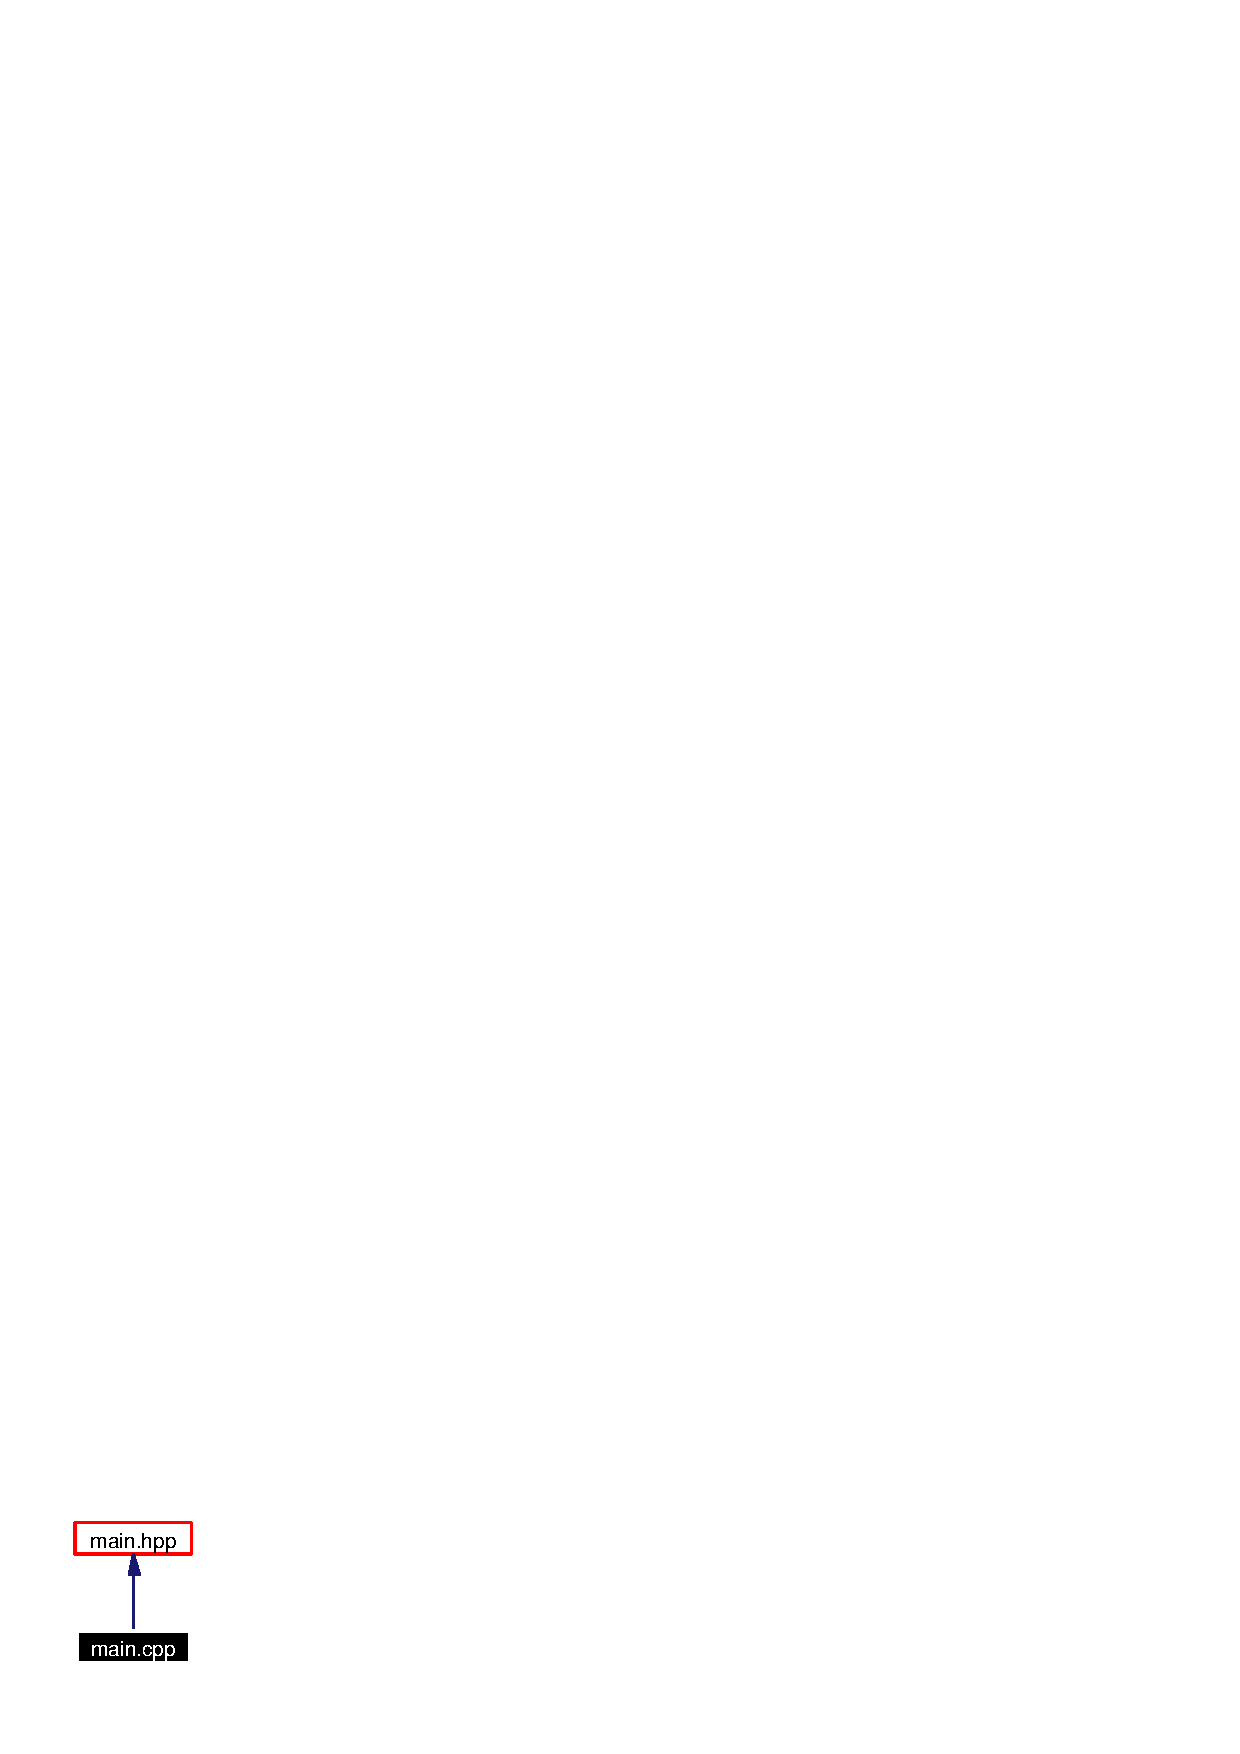
\includegraphics[width=46pt]{main_8cpp__incl}
\end{center}
\end{figure}
\subsection*{Functions}
\begin{CompactItemize}
\item 
int {\bf sdl\_\-start} ({\bf Log\-Engine} \&log)
\item 
void {\bf sdl\_\-stop} (void)
\item 
void {\bf run\-Gui\-Loop} ({\bf World\-Data} \&world\-Data, {\bf System\-Data} \&system\-Data, {\bf Log\-Engine} \&log, {\bf Data\-Engine} \&data, {\bf Input\-Engine} \&input, {\bf Graphics\-Engine} \&graphics, {\bf Physics\-Engine} \&physics, {\bf Gui\-Engine} \&gui)
\item 
void {\bf run\-Sim\-Loop} ({\bf World\-Data} \&world\-Data, {\bf System\-Data} \&system\-Data, {\bf Log\-Engine} \&log, {\bf Data\-Engine} \&data, {\bf Input\-Engine} \&input, {\bf Graphics\-Engine} \&graphics, {\bf Physics\-Engine} \&physics, {\bf Gui\-Engine} \&gui)
\item 
void {\bf initialize\-Sim\-Loop} ({\bf World\-Data} \&world\-Data, {\bf System\-Data} \&system\-Data, {\bf Log\-Engine} \&log, {\bf Data\-Engine} \&data, {\bf Input\-Engine} \&input, {\bf Graphics\-Engine} \&graphics, {\bf Physics\-Engine} \&physics, {\bf Gui\-Engine} \&gui)
\item 
void {\bf shutdown\-Sim\-Loop} ({\bf World\-Data} \&world\-Data, {\bf System\-Data} \&system\-Data, {\bf Log\-Engine} \&log, {\bf Data\-Engine} \&data, {\bf Input\-Engine} \&input, {\bf Graphics\-Engine} \&graphics, {\bf Physics\-Engine} \&physics, {\bf Gui\-Engine} \&gui)
\item 
void {\bf initialize\-Gui\-Loop} ({\bf World\-Data} \&world\-Data, {\bf System\-Data} \&system\-Data, {\bf Log\-Engine} \&log, {\bf Data\-Engine} \&data, {\bf Input\-Engine} \&input, {\bf Graphics\-Engine} \&graphics, {\bf Physics\-Engine} \&physics, {\bf Gui\-Engine} \&gui)
\item 
void {\bf shutdown\-Gui\-Loop} ({\bf World\-Data} \&world\-Data, {\bf System\-Data} \&system\-Data, {\bf Log\-Engine} \&log, {\bf Data\-Engine} \&data, {\bf Input\-Engine} \&input, {\bf Graphics\-Engine} \&graphics, {\bf Physics\-Engine} \&physics, {\bf Gui\-Engine} \&gui)
\item 
void {\bf initialize\-Main\-Loop} ({\bf World\-Data} \&world\-Data, {\bf System\-Data} \&system\-Data, {\bf Log\-Engine} \&log, {\bf Data\-Engine} \&data, {\bf Input\-Engine} \&input, {\bf Graphics\-Engine} \&graphics, {\bf Physics\-Engine} \&physics, {\bf Gui\-Engine} \&gui)
\item 
void {\bf shutdown\-Main\-Loop} ({\bf World\-Data} \&world\-Data, {\bf System\-Data} \&system\-Data, {\bf Log\-Engine} \&log, {\bf Data\-Engine} \&data, {\bf Input\-Engine} \&input, {\bf Graphics\-Engine} \&graphics, {\bf Physics\-Engine} \&physics, {\bf Gui\-Engine} \&gui)
\item 
int {\bf main} (int argc, char $\ast$$\ast$argv)
\end{CompactItemize}


\subsection{Function Documentation}
\index{main.cpp@{main.cpp}!initializeGuiLoop@{initializeGuiLoop}}
\index{initializeGuiLoop@{initializeGuiLoop}!main.cpp@{main.cpp}}
\subsubsection{\setlength{\rightskip}{0pt plus 5cm}void initialize\-Gui\-Loop ({\bf World\-Data} \& {\em world\-Data}, {\bf System\-Data} \& {\em system\-Data}, {\bf Log\-Engine} \& {\em log}, {\bf Data\-Engine} \& {\em data}, {\bf Input\-Engine} \& {\em input}, {\bf Graphics\-Engine} \& {\em graphics}, {\bf Physics\-Engine} \& {\em physics}, {\bf Gui\-Engine} \& {\em gui})}\label{main_8cpp_a6}


\index{main.cpp@{main.cpp}!initializeMainLoop@{initializeMainLoop}}
\index{initializeMainLoop@{initializeMainLoop}!main.cpp@{main.cpp}}
\subsubsection{\setlength{\rightskip}{0pt plus 5cm}void initialize\-Main\-Loop ({\bf World\-Data} \& {\em world\-Data}, {\bf System\-Data} \& {\em system\-Data}, {\bf Log\-Engine} \& {\em log}, {\bf Data\-Engine} \& {\em data}, {\bf Input\-Engine} \& {\em input}, {\bf Graphics\-Engine} \& {\em graphics}, {\bf Physics\-Engine} \& {\em physics}, {\bf Gui\-Engine} \& {\em gui})}\label{main_8cpp_a8}


\index{main.cpp@{main.cpp}!initializeSimLoop@{initializeSimLoop}}
\index{initializeSimLoop@{initializeSimLoop}!main.cpp@{main.cpp}}
\subsubsection{\setlength{\rightskip}{0pt plus 5cm}void initialize\-Sim\-Loop ({\bf World\-Data} \& {\em world\-Data}, {\bf System\-Data} \& {\em system\-Data}, {\bf Log\-Engine} \& {\em log}, {\bf Data\-Engine} \& {\em data}, {\bf Input\-Engine} \& {\em input}, {\bf Graphics\-Engine} \& {\em graphics}, {\bf Physics\-Engine} \& {\em physics}, {\bf Gui\-Engine} \& {\em gui})}\label{main_8cpp_a4}


\index{main.cpp@{main.cpp}!main@{main}}
\index{main@{main}!main.cpp@{main.cpp}}
\subsubsection{\setlength{\rightskip}{0pt plus 5cm}int main (int {\em argc}, char $\ast$$\ast$ {\em argv})}\label{main_8cpp_a10}


\index{main.cpp@{main.cpp}!runGuiLoop@{runGuiLoop}}
\index{runGuiLoop@{runGuiLoop}!main.cpp@{main.cpp}}
\subsubsection{\setlength{\rightskip}{0pt plus 5cm}void run\-Gui\-Loop ({\bf World\-Data} \& {\em world\-Data}, {\bf System\-Data} \& {\em system\-Data}, {\bf Log\-Engine} \& {\em log}, {\bf Data\-Engine} \& {\em data}, {\bf Input\-Engine} \& {\em input}, {\bf Graphics\-Engine} \& {\em graphics}, {\bf Physics\-Engine} \& {\em physics}, {\bf Gui\-Engine} \& {\em gui})}\label{main_8cpp_a2}


\index{main.cpp@{main.cpp}!runSimLoop@{runSimLoop}}
\index{runSimLoop@{runSimLoop}!main.cpp@{main.cpp}}
\subsubsection{\setlength{\rightskip}{0pt plus 5cm}void run\-Sim\-Loop ({\bf World\-Data} \& {\em world\-Data}, {\bf System\-Data} \& {\em system\-Data}, {\bf Log\-Engine} \& {\em log}, {\bf Data\-Engine} \& {\em data}, {\bf Input\-Engine} \& {\em input}, {\bf Graphics\-Engine} \& {\em graphics}, {\bf Physics\-Engine} \& {\em physics}, {\bf Gui\-Engine} \& {\em gui})}\label{main_8cpp_a3}


\index{main.cpp@{main.cpp}!sdl_start@{sdl\_\-start}}
\index{sdl_start@{sdl\_\-start}!main.cpp@{main.cpp}}
\subsubsection{\setlength{\rightskip}{0pt plus 5cm}int sdl\_\-start ({\bf Log\-Engine} \& {\em log})}\label{main_8cpp_a0}


\index{main.cpp@{main.cpp}!sdl_stop@{sdl\_\-stop}}
\index{sdl_stop@{sdl\_\-stop}!main.cpp@{main.cpp}}
\subsubsection{\setlength{\rightskip}{0pt plus 5cm}void sdl\_\-stop (void)}\label{main_8cpp_a1}


\index{main.cpp@{main.cpp}!shutdownGuiLoop@{shutdownGuiLoop}}
\index{shutdownGuiLoop@{shutdownGuiLoop}!main.cpp@{main.cpp}}
\subsubsection{\setlength{\rightskip}{0pt plus 5cm}void shutdown\-Gui\-Loop ({\bf World\-Data} \& {\em world\-Data}, {\bf System\-Data} \& {\em system\-Data}, {\bf Log\-Engine} \& {\em log}, {\bf Data\-Engine} \& {\em data}, {\bf Input\-Engine} \& {\em input}, {\bf Graphics\-Engine} \& {\em graphics}, {\bf Physics\-Engine} \& {\em physics}, {\bf Gui\-Engine} \& {\em gui})}\label{main_8cpp_a7}


\index{main.cpp@{main.cpp}!shutdownMainLoop@{shutdownMainLoop}}
\index{shutdownMainLoop@{shutdownMainLoop}!main.cpp@{main.cpp}}
\subsubsection{\setlength{\rightskip}{0pt plus 5cm}void shutdown\-Main\-Loop ({\bf World\-Data} \& {\em world\-Data}, {\bf System\-Data} \& {\em system\-Data}, {\bf Log\-Engine} \& {\em log}, {\bf Data\-Engine} \& {\em data}, {\bf Input\-Engine} \& {\em input}, {\bf Graphics\-Engine} \& {\em graphics}, {\bf Physics\-Engine} \& {\em physics}, {\bf Gui\-Engine} \& {\em gui})}\label{main_8cpp_a9}


\index{main.cpp@{main.cpp}!shutdownSimLoop@{shutdownSimLoop}}
\index{shutdownSimLoop@{shutdownSimLoop}!main.cpp@{main.cpp}}
\subsubsection{\setlength{\rightskip}{0pt plus 5cm}void shutdown\-Sim\-Loop ({\bf World\-Data} \& {\em world\-Data}, {\bf System\-Data} \& {\em system\-Data}, {\bf Log\-Engine} \& {\em log}, {\bf Data\-Engine} \& {\em data}, {\bf Input\-Engine} \& {\em input}, {\bf Graphics\-Engine} \& {\em graphics}, {\bf Physics\-Engine} \& {\em physics}, {\bf Gui\-Engine} \& {\em gui})}\label{main_8cpp_a5}



\section{src/main.hpp File Reference}
\label{main_8hpp}\index{src/main.hpp@{src/main.hpp}}
{\tt \#include $<$stdlib.h$>$}\par
{\tt \#include \char`\"{}SDL.h\char`\"{}}\par
{\tt \#include \char`\"{}world.hpp\char`\"{}}\par
{\tt \#include \char`\"{}system.hpp\char`\"{}}\par
{\tt \#include \char`\"{}log\-Engine.hpp\char`\"{}}\par
{\tt \#include \char`\"{}data\-Engine.hpp\char`\"{}}\par
{\tt \#include \char`\"{}input\-Engine.hpp\char`\"{}}\par
{\tt \#include \char`\"{}graphics\-Engine.hpp\char`\"{}}\par
{\tt \#include \char`\"{}physics\-Engine.hpp\char`\"{}}\par
{\tt \#include \char`\"{}gui\-Engine.hpp\char`\"{}}\par


Include dependency graph for main.hpp:\begin{figure}[H]
\begin{center}
\leavevmode
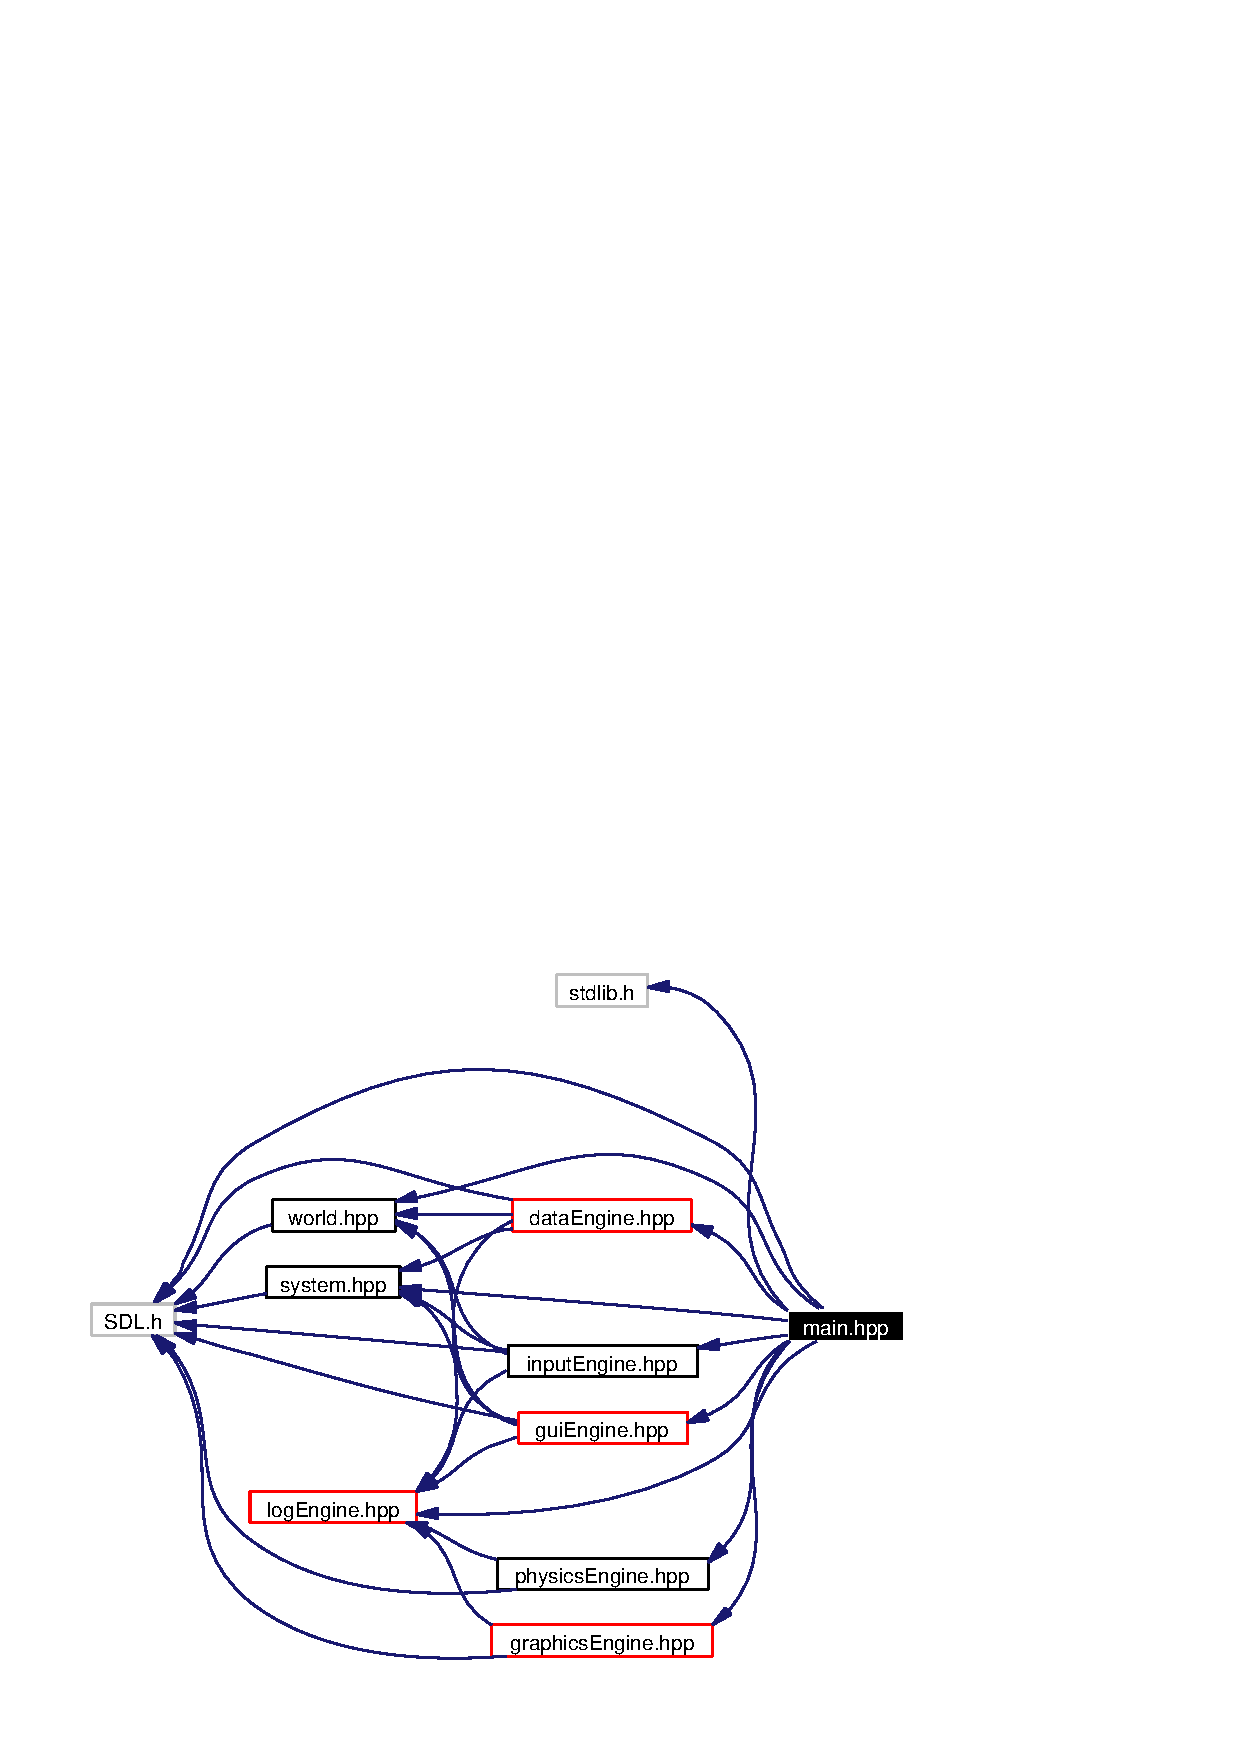
\includegraphics[width=221pt]{main_8hpp__incl}
\end{center}
\end{figure}


This graph shows which files directly or indirectly include this file:\begin{figure}[H]
\begin{center}
\leavevmode
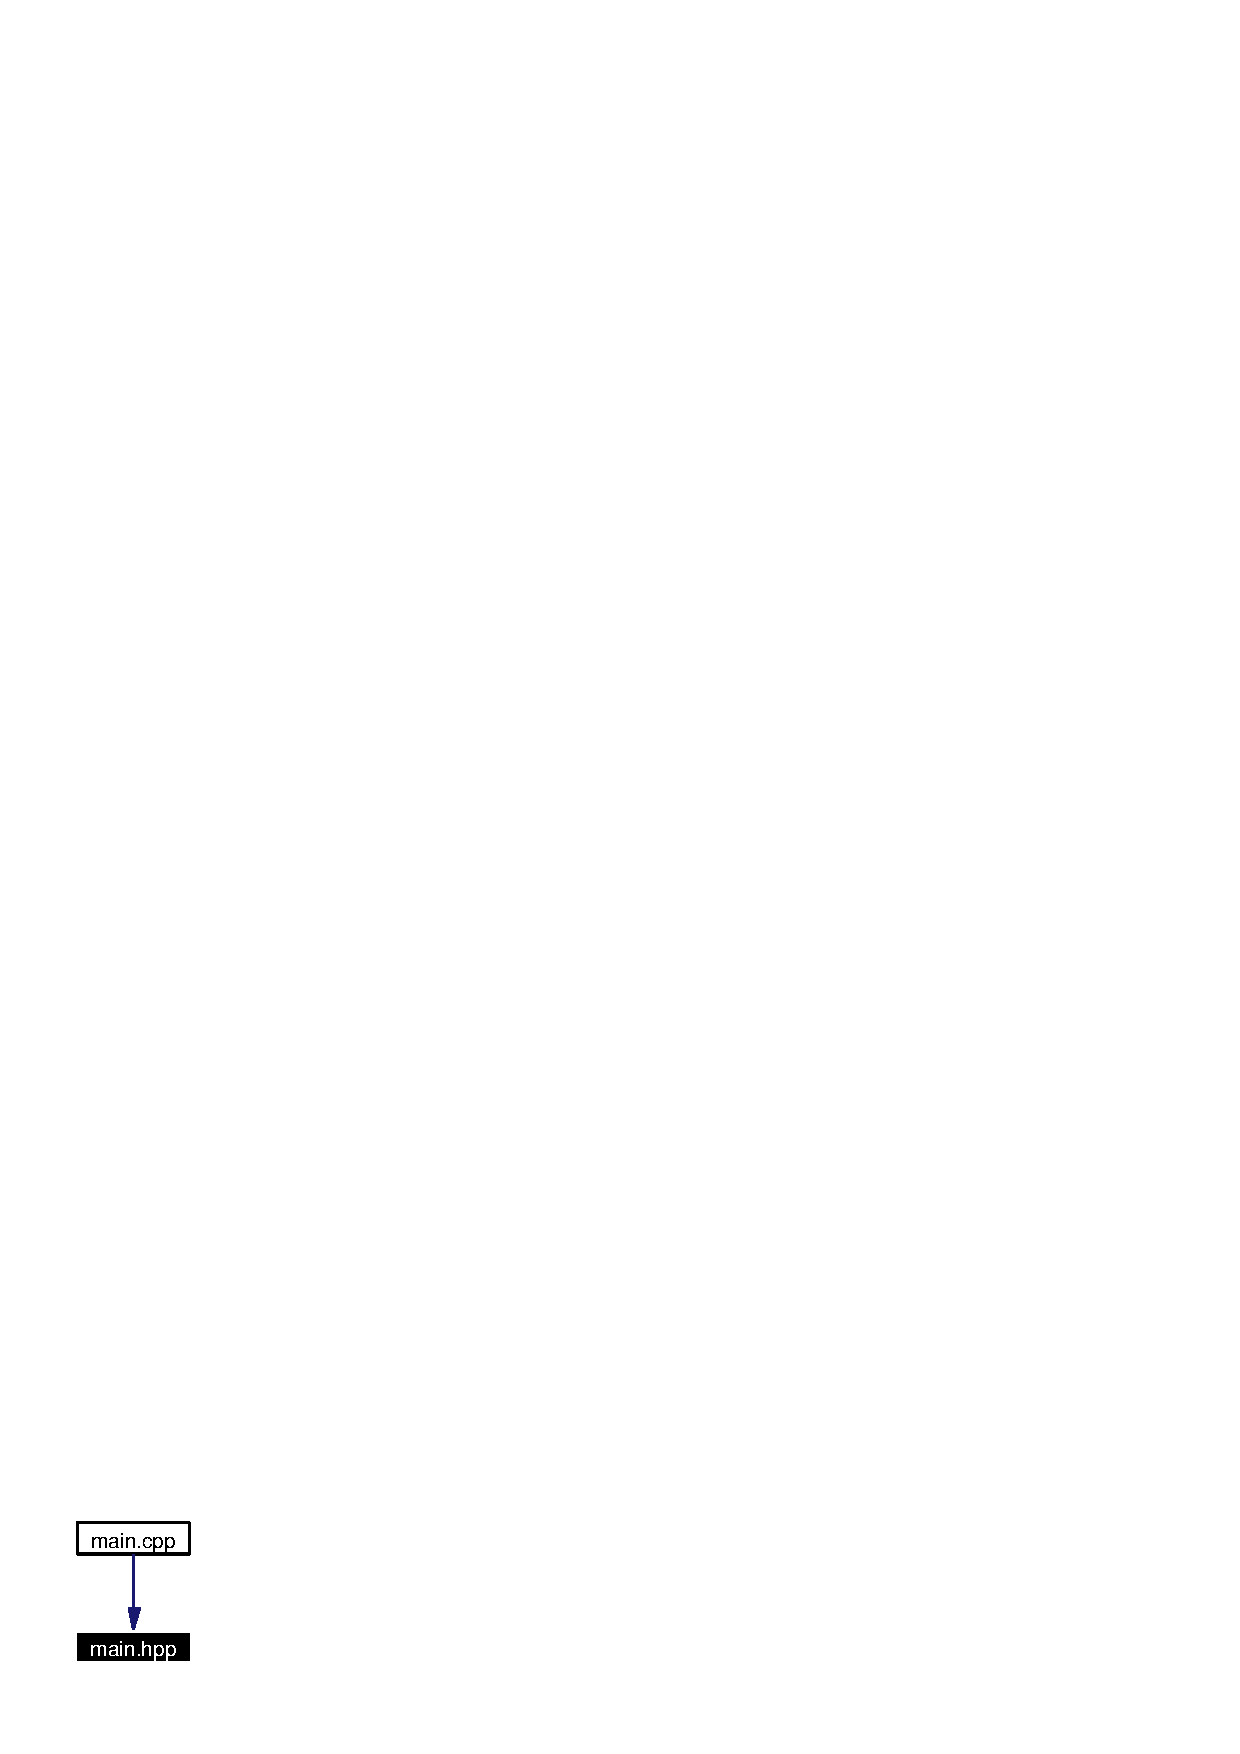
\includegraphics[width=46pt]{main_8hpp__dep__incl}
\end{center}
\end{figure}

\section{src/physics/physics\-Engine.cpp File Reference}
\label{physicsEngine_8cpp}\index{src/physics/physicsEngine.cpp@{src/physics/physicsEngine.cpp}}
{\tt \#include \char`\"{}system.hpp\char`\"{}}\par
{\tt \#include \char`\"{}world.hpp\char`\"{}}\par
{\tt \#include \char`\"{}physics\-Engine.hpp\char`\"{}}\par
{\tt \#include \char`\"{}test\_\-ode.cpp\char`\"{}}\par
{\tt \#include $<$math.h$>$}\par


Include dependency graph for physics\-Engine.cpp:\begin{figure}[H]
\begin{center}
\leavevmode
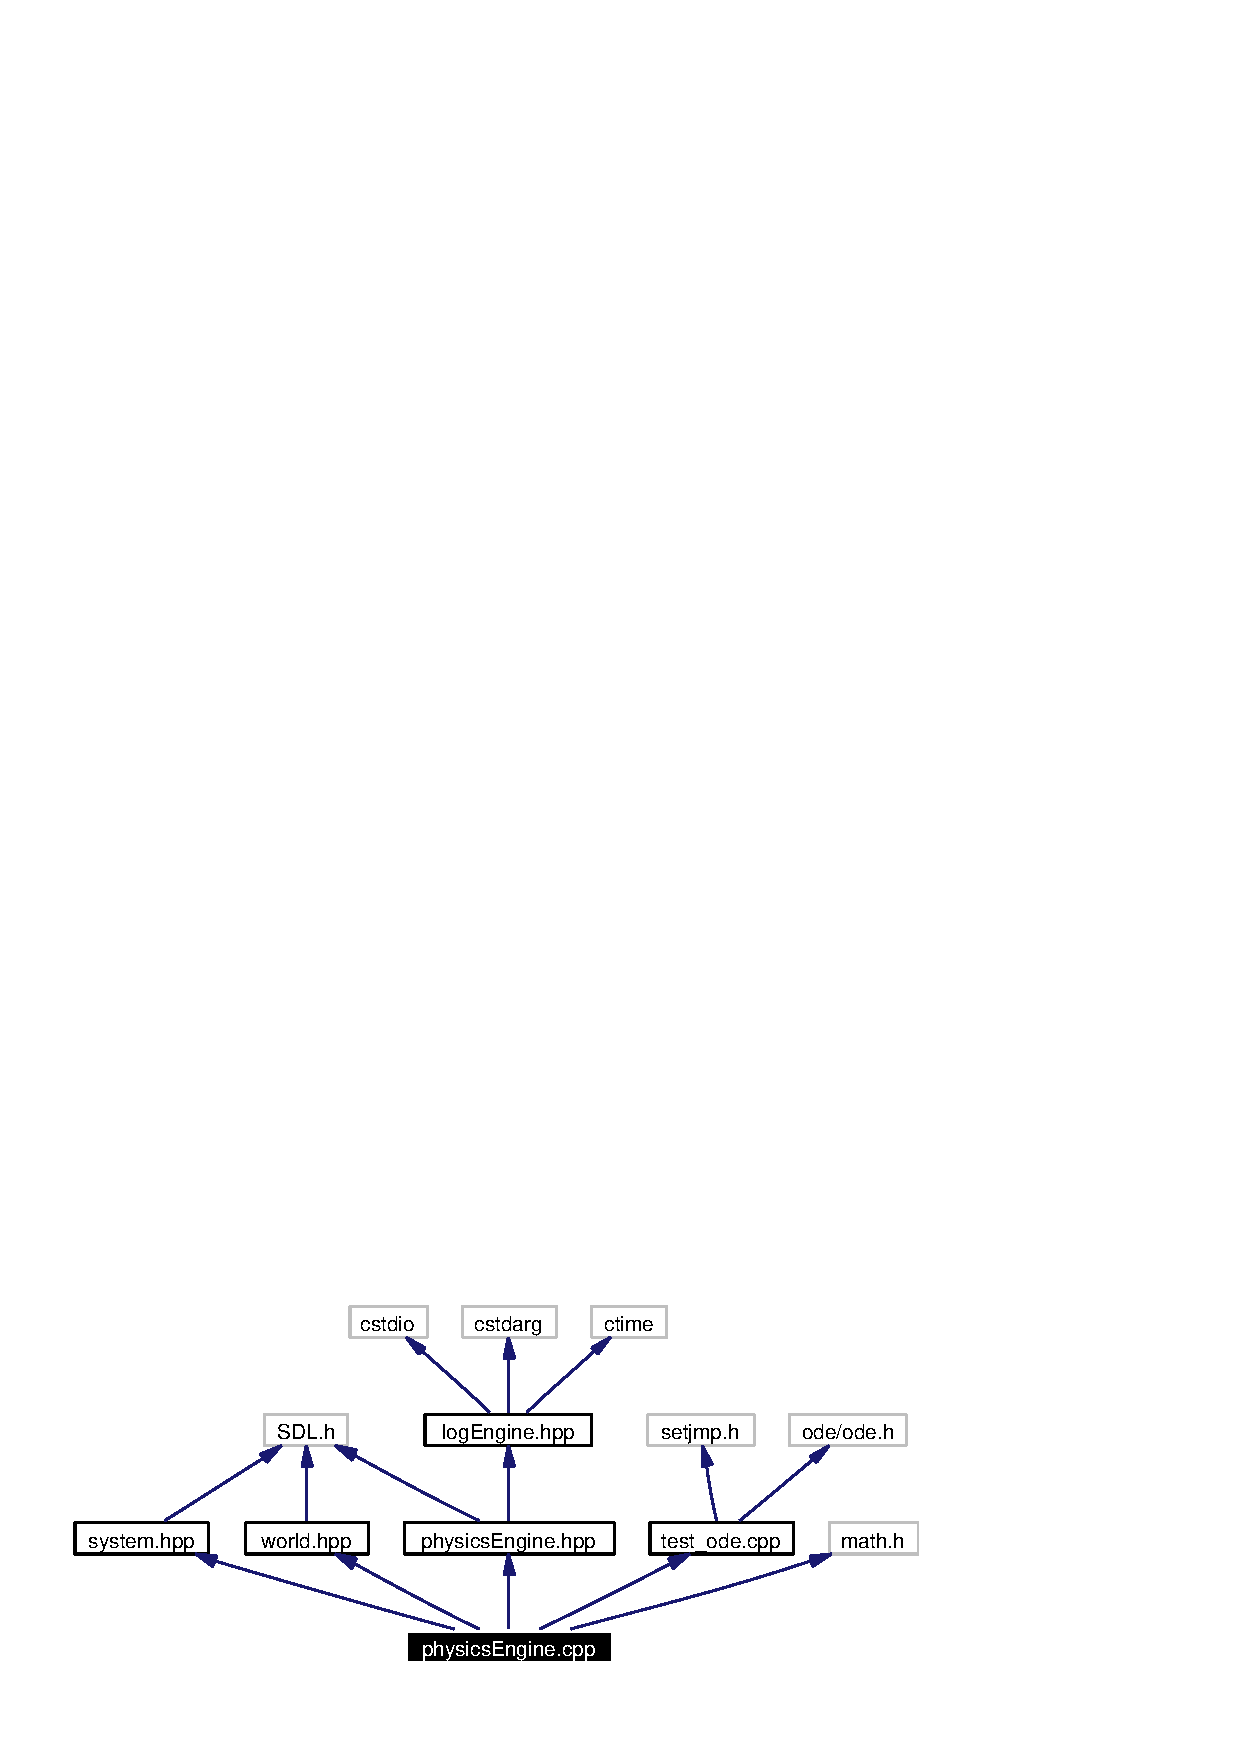
\includegraphics[width=220pt]{physicsEngine_8cpp__incl}
\end{center}
\end{figure}

\section{src/physics/physics\-Engine.hpp File Reference}
\label{physicsEngine_8hpp}\index{src/physics/physicsEngine.hpp@{src/physics/physicsEngine.hpp}}
{\tt \#include \char`\"{}log\-Engine.hpp\char`\"{}}\par
{\tt \#include \char`\"{}SDL.h\char`\"{}}\par


Include dependency graph for physics\-Engine.hpp:\begin{figure}[H]
\begin{center}
\leavevmode
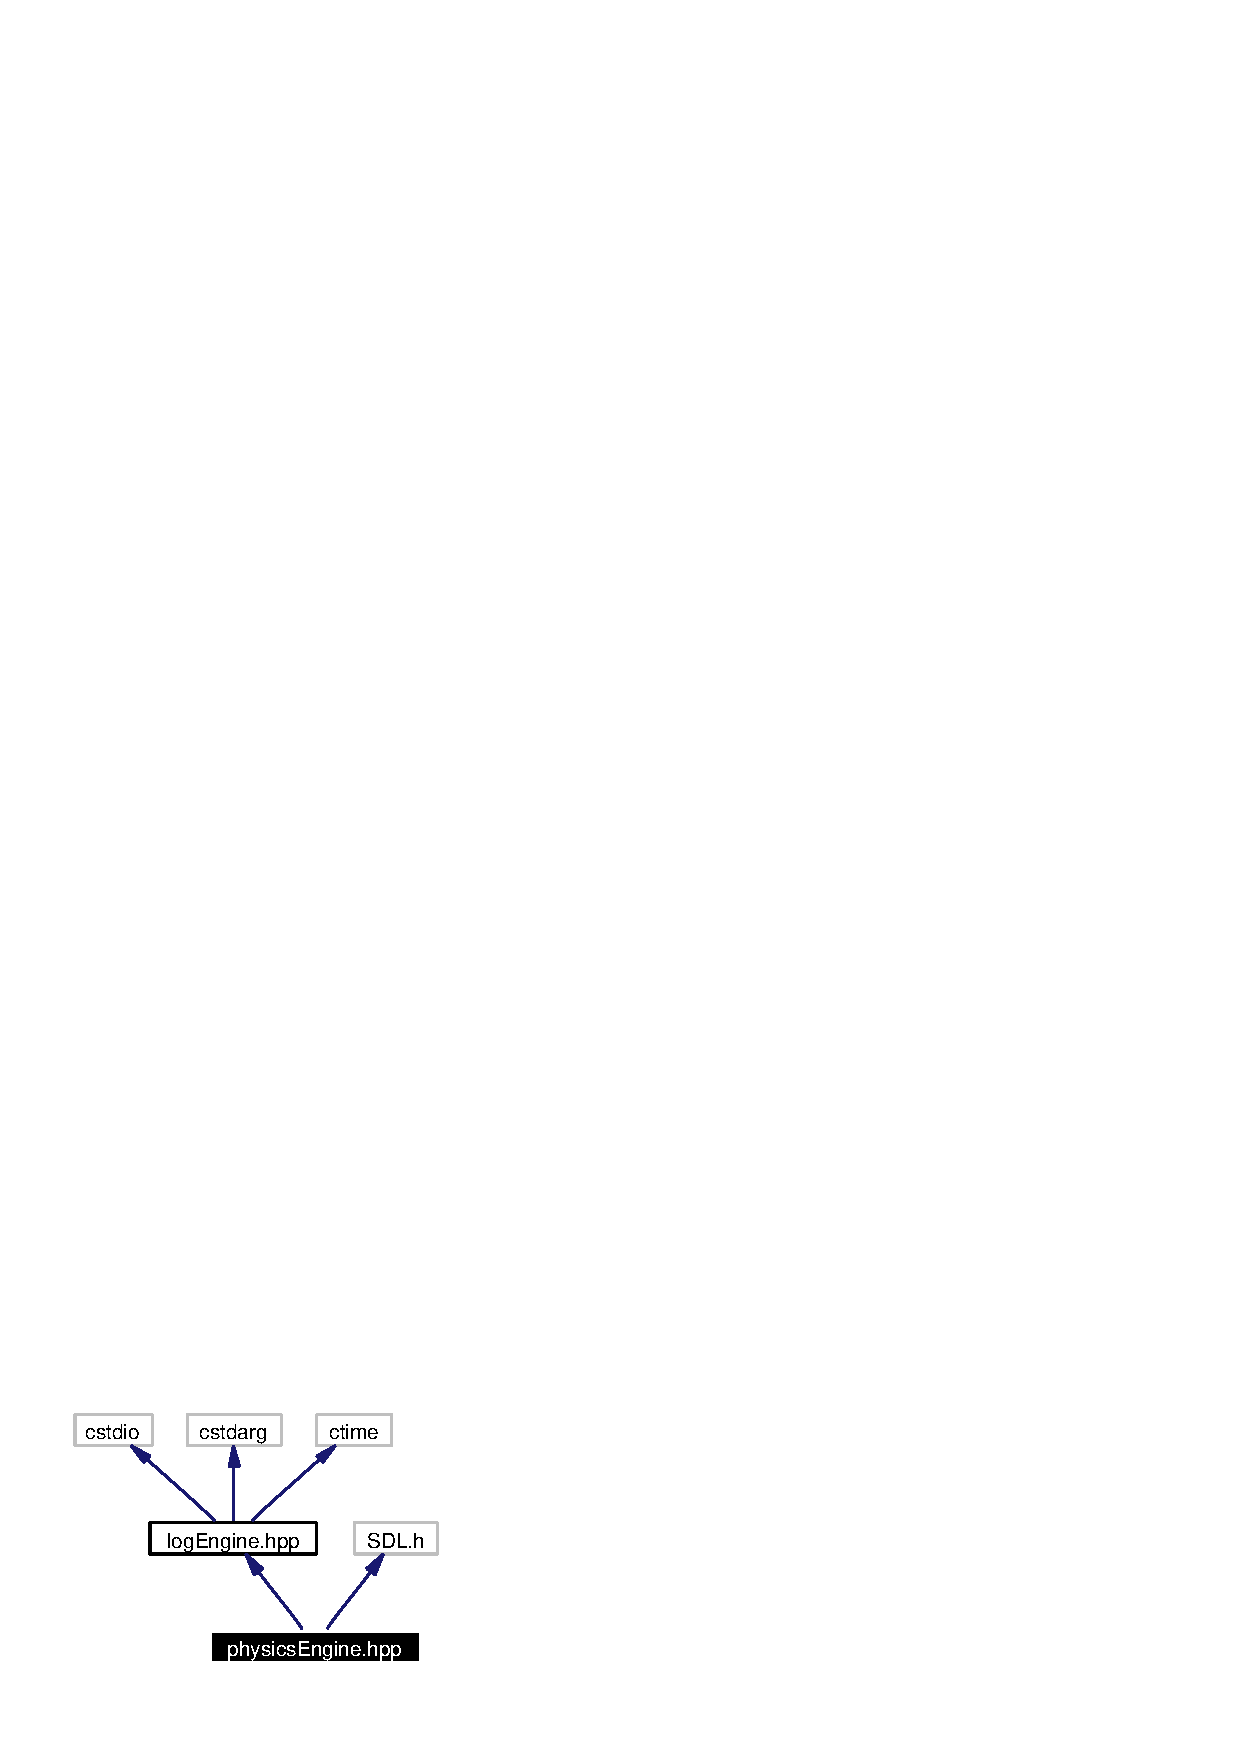
\includegraphics[width=105pt]{physicsEngine_8hpp__incl}
\end{center}
\end{figure}


This graph shows which files directly or indirectly include this file:\begin{figure}[H]
\begin{center}
\leavevmode
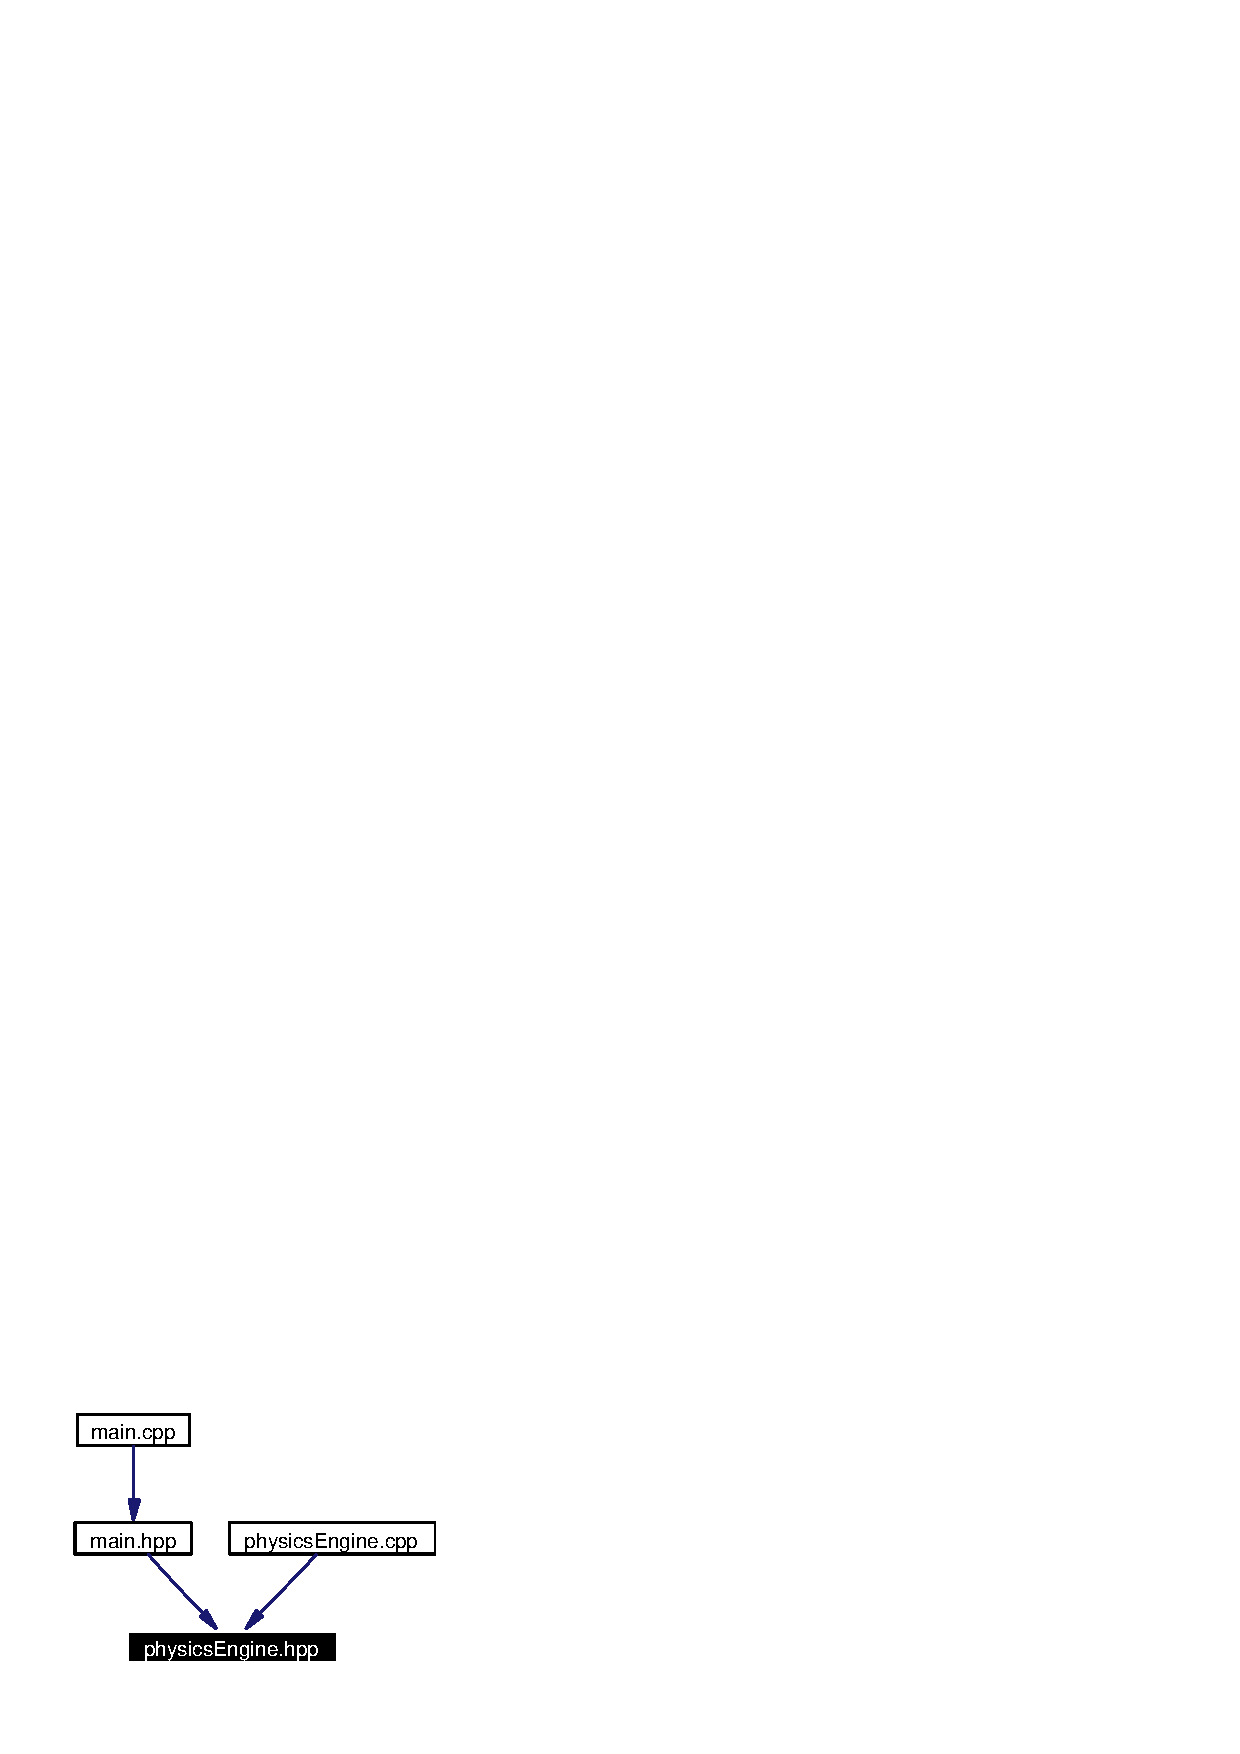
\includegraphics[width=104pt]{physicsEngine_8hpp__dep__incl}
\end{center}
\end{figure}
\subsection*{Classes}
\begin{CompactItemize}
\item 
class {\bf Physics\-Engine}
\end{CompactItemize}

\section{src/physics/test\_\-ode.cpp File Reference}
\label{test__ode_8cpp}\index{src/physics/test_ode.cpp@{src/physics/test\_\-ode.cpp}}
{\tt \#include $<$setjmp.h$>$}\par
{\tt \#include $<$ode/ode.h$>$}\par


Include dependency graph for test\_\-ode.cpp:\begin{figure}[H]
\begin{center}
\leavevmode
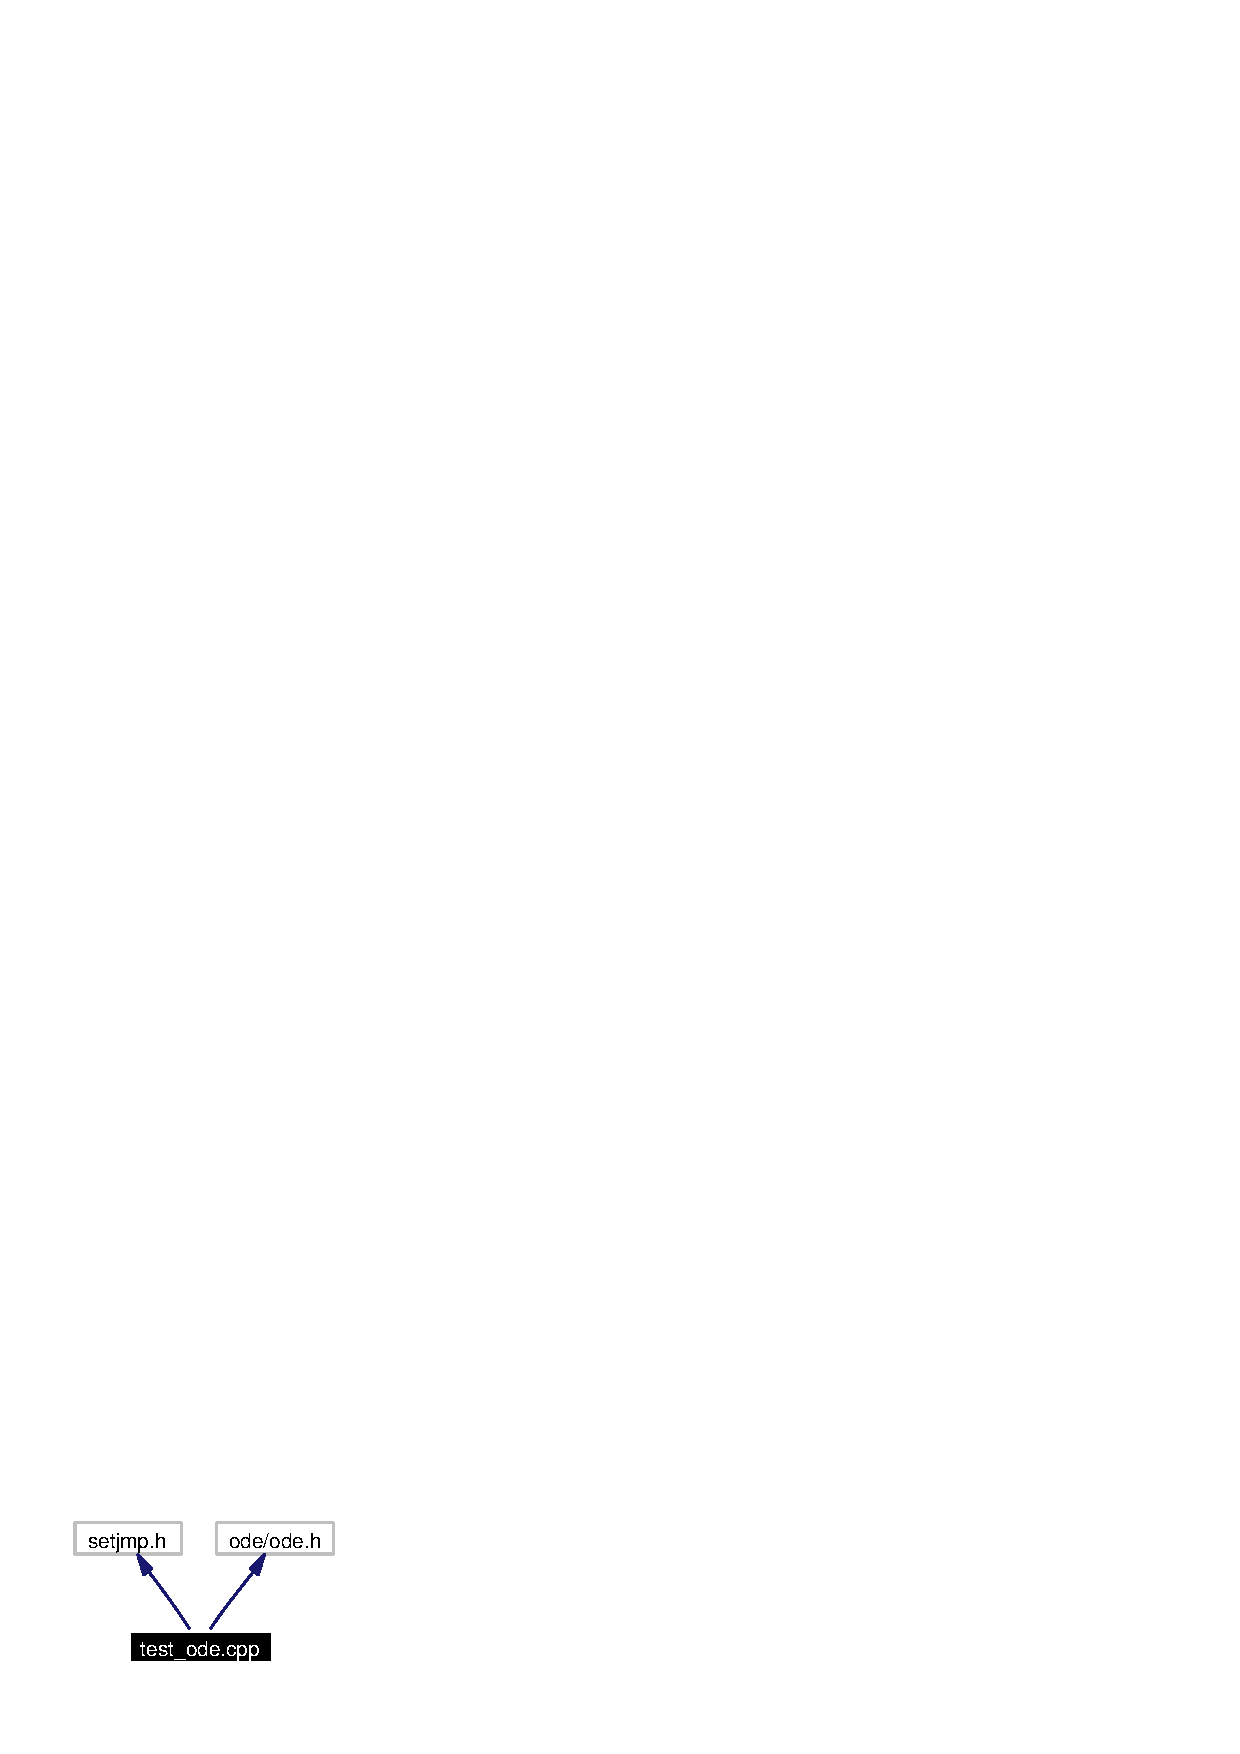
\includegraphics[width=80pt]{test__ode_8cpp__incl}
\end{center}
\end{figure}


This graph shows which files directly or indirectly include this file:\begin{figure}[H]
\begin{center}
\leavevmode
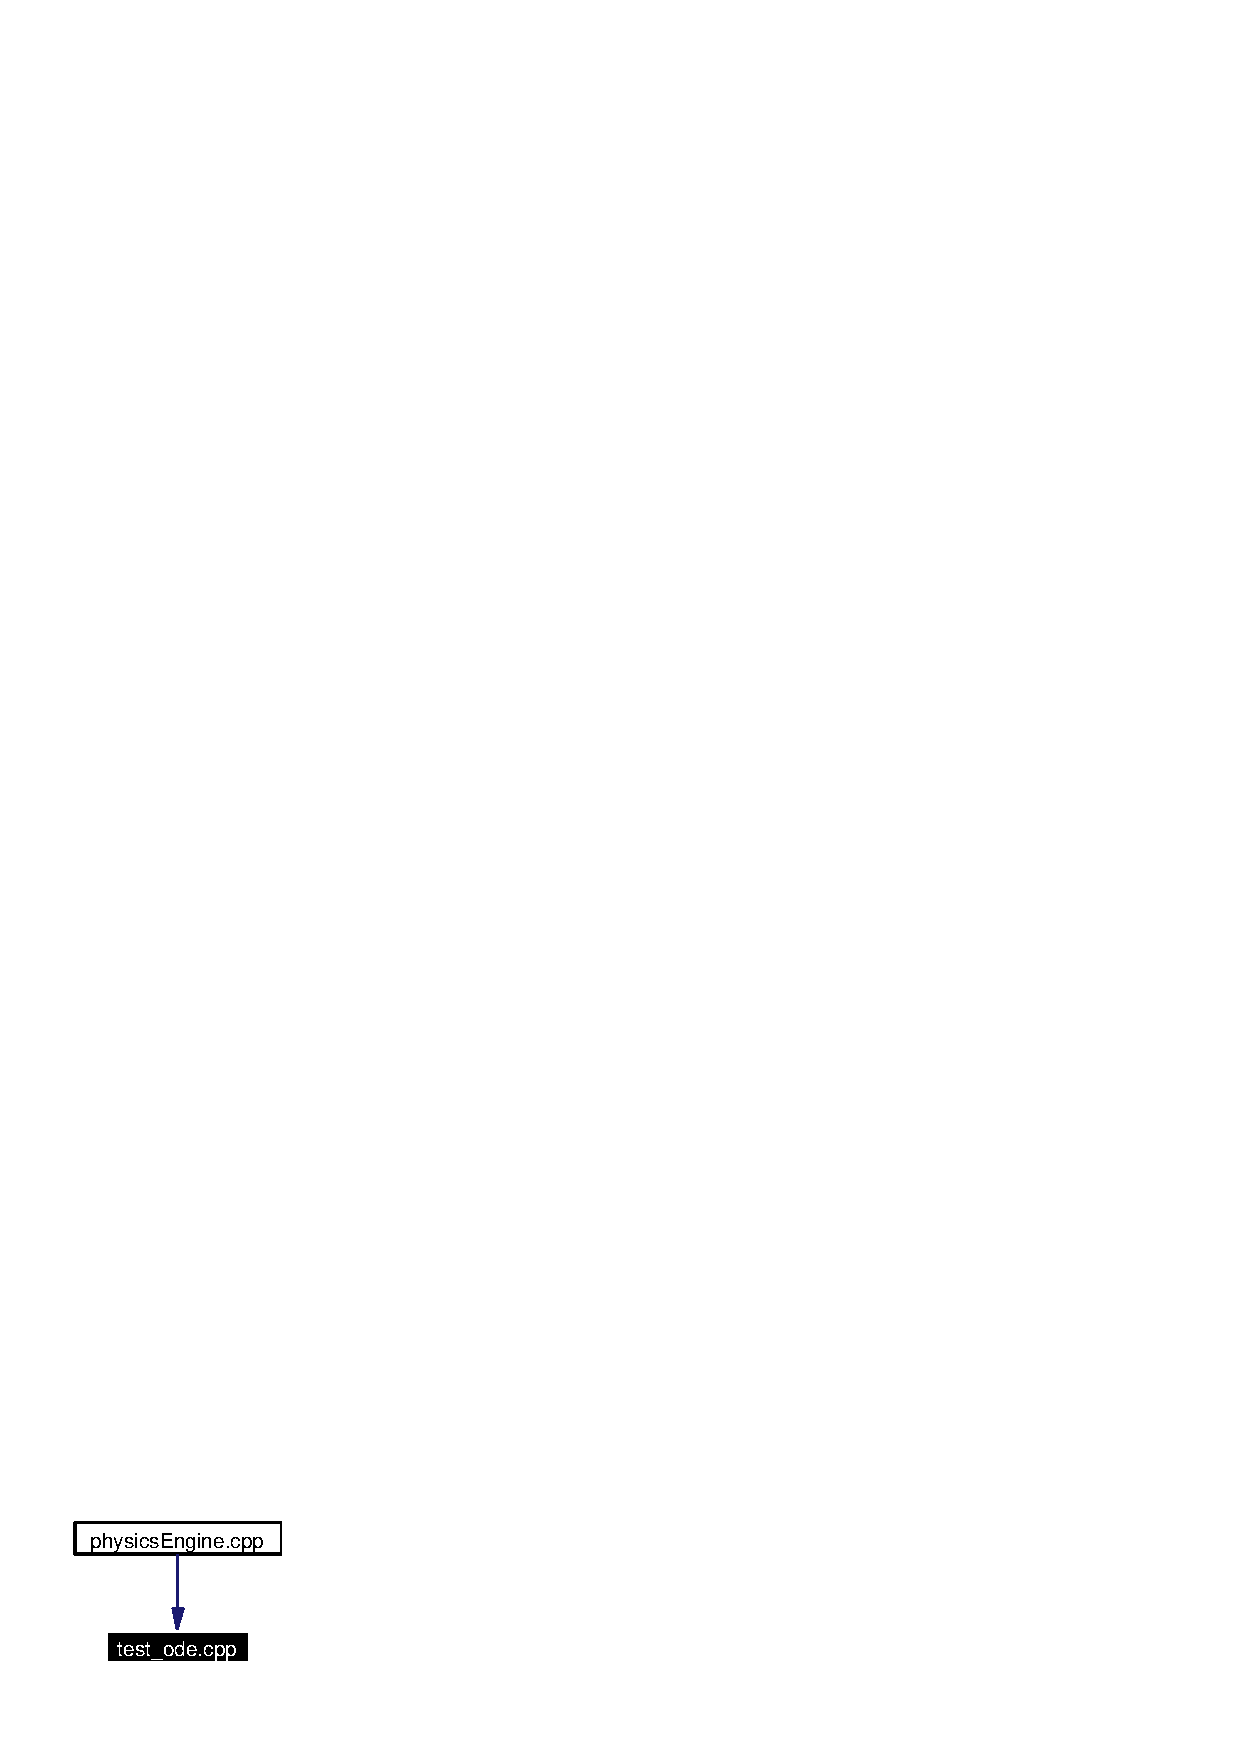
\includegraphics[width=67pt]{test__ode_8cpp__dep__incl}
\end{center}
\end{figure}
\subsection*{Defines}
\begin{CompactItemize}
\item 
\#define {\bf \_\-A}(i, j)\ A[(i)$\ast$4+(j)]
\item 
\#define {\bf \_\-I}(i, j)\ I[(i)$\ast$4+(j)]
\item 
\#define {\bf \_\-R}(i, j)\ R[(i)$\ast$4+(j)]
\item 
\#define {\bf HEADER}\ printf (\char`\"{}\%s:\%d$\backslash$n\char`\"{},\_\-\_\-FILE\_\-\_\-,\_\-\_\-LINE\_\-\_\-);
\item 
\#define {\bf TRAP\_\-MESSAGE}(do, ifnomsg, ifmsg)
\item 
\#define {\bf MSIZE}\ 21
\item 
\#define {\bf MSIZE4}\ 24
\item 
\#define {\bf NUMP}\ 10
\end{CompactItemize}
\subsection*{Functions}
\begin{CompactItemize}
\item 
void {\bf my\-Message\-Function} (int num, const char $\ast$msg, va\_\-list ap)
\item 
int {\bf cmp} (d\-Real a, d\-Real b)
\item 
int {\bf cmp\-Identity\-Mat3} (d\-Matrix3 A)
\item 
void {\bf transpose3x3} (d\-Matrix3 A)
\item 
void {\bf test\-Random\-Number\-Generator} ()
\item 
void {\bf test\-Infinity} ()
\item 
void {\bf test\-Pad} ()
\item 
void {\bf test\-Cross\-Product} ()
\item 
void {\bf test\-Set\-Zero} ()
\item 
void {\bf test\-Normalize3} ()
\item 
void {\bf test\-Plane\-Space} ()
\item 
void {\bf test\-Matrix\-Multiply} ()
\item 
void {\bf test\-Small\-Matrix\-Multiply} ()
\item 
void {\bf test\-Cholesky\-Factorization} ()
\item 
void {\bf test\-Cholesky\-Solve} ()
\item 
void {\bf test\-Invert\-PDMatrix} ()
\item 
void {\bf test\-Is\-Positive\-Definite} ()
\item 
void {\bf test\-Fast\-LDLTFactorization} ()
\item 
void {\bf test\-Solve\-LDLT} ()
\item 
void {\bf test\-LDLTAdd\-TL} ()
\item 
void {\bf test\-LDLTRemove} ()
\item 
void {\bf print\-Mass\-Params} (d\-Mass $\ast$m)
\item 
void {\bf compare\-Mass\-Params} (d\-Mass $\ast$m1, d\-Mass $\ast$m2, char $\ast$msg)
\item 
void {\bf compute\-Mass\-Params} (d\-Mass $\ast$m, d\-Real q[NUMP][3], d\-Real pm[NUMP])
\item 
void {\bf test\-Mass\-Functions} ()
\item 
void {\bf make\-Random\-Rotation} (d\-Matrix3 R)
\item 
void {\bf test\-Rto\-Qand\-Qto\-R} ()
\item 
void {\bf test\-Quaternion\-Multiply} ()
\item 
void {\bf test\-Rotation\-Functions} ()
\item 
void {\bf d\-Test\-Data\-Structures} ()
\item 
void {\bf d\-Test\-Matrix\-Comparison} ()
\item 
void {\bf d\-Test\-Solve\-LCP} ()
\item 
int {\bf test\-Ode} (void)
\item 
void {\bf test\-Ode2} (void)
\end{CompactItemize}
\subsection*{Variables}
\begin{CompactItemize}
\item 
jmp\_\-buf {\bf jump\_\-buffer}
\end{CompactItemize}


\subsection{Define Documentation}
\index{test_ode.cpp@{test\_\-ode.cpp}!_A@{\_\-A}}
\index{_A@{\_\-A}!test_ode.cpp@{test\_\-ode.cpp}}
\subsubsection{\setlength{\rightskip}{0pt plus 5cm}\#define \_\-A(i, j)\ A[(i)$\ast$4+(j)]}\label{test__ode_8cpp_a0}


\index{test_ode.cpp@{test\_\-ode.cpp}!_I@{\_\-I}}
\index{_I@{\_\-I}!test_ode.cpp@{test\_\-ode.cpp}}
\subsubsection{\setlength{\rightskip}{0pt plus 5cm}\#define \_\-I(i, j)\ I[(i)$\ast$4+(j)]}\label{test__ode_8cpp_a1}


\index{test_ode.cpp@{test\_\-ode.cpp}!_R@{\_\-R}}
\index{_R@{\_\-R}!test_ode.cpp@{test\_\-ode.cpp}}
\subsubsection{\setlength{\rightskip}{0pt plus 5cm}\#define \_\-R(i, j)\ R[(i)$\ast$4+(j)]}\label{test__ode_8cpp_a2}


\index{test_ode.cpp@{test\_\-ode.cpp}!HEADER@{HEADER}}
\index{HEADER@{HEADER}!test_ode.cpp@{test\_\-ode.cpp}}
\subsubsection{\setlength{\rightskip}{0pt plus 5cm}\#define HEADER\ printf (\char`\"{}\%s:\%d$\backslash$n\char`\"{},\_\-\_\-FILE\_\-\_\-,\_\-\_\-LINE\_\-\_\-);}\label{test__ode_8cpp_a3}


\index{test_ode.cpp@{test\_\-ode.cpp}!MSIZE@{MSIZE}}
\index{MSIZE@{MSIZE}!test_ode.cpp@{test\_\-ode.cpp}}
\subsubsection{\setlength{\rightskip}{0pt plus 5cm}\#define MSIZE\ 21}\label{test__ode_8cpp_a5}


\index{test_ode.cpp@{test\_\-ode.cpp}!MSIZE4@{MSIZE4}}
\index{MSIZE4@{MSIZE4}!test_ode.cpp@{test\_\-ode.cpp}}
\subsubsection{\setlength{\rightskip}{0pt plus 5cm}\#define MSIZE4\ 24}\label{test__ode_8cpp_a6}


\index{test_ode.cpp@{test\_\-ode.cpp}!NUMP@{NUMP}}
\index{NUMP@{NUMP}!test_ode.cpp@{test\_\-ode.cpp}}
\subsubsection{\setlength{\rightskip}{0pt plus 5cm}\#define NUMP\ 10}\label{test__ode_8cpp_a7}


\index{test_ode.cpp@{test\_\-ode.cpp}!TRAP_MESSAGE@{TRAP\_\-MESSAGE}}
\index{TRAP_MESSAGE@{TRAP\_\-MESSAGE}!test_ode.cpp@{test\_\-ode.cpp}}
\subsubsection{\setlength{\rightskip}{0pt plus 5cm}\#define TRAP\_\-MESSAGE(do, ifnomsg, ifmsg)}\label{test__ode_8cpp_a4}


{\bf Value:}

\footnotesize\begin{verbatim}dSetMessageHandler (&myMessageFunction); \
  if (setjmp (jump_buffer)) { \
    dSetMessageHandler (0); \
    ifmsg ; \
  } \
  else { \
    dSetMessageHandler (&myMessageFunction); \
    do ; \
    ifnomsg ; \
  } \
  dSetMessageHandler (0);
\end{verbatim}\normalsize 


\subsection{Function Documentation}
\index{test_ode.cpp@{test\_\-ode.cpp}!cmp@{cmp}}
\index{cmp@{cmp}!test_ode.cpp@{test\_\-ode.cpp}}
\subsubsection{\setlength{\rightskip}{0pt plus 5cm}int cmp (d\-Real {\em a}, d\-Real {\em b})}\label{test__ode_8cpp_a10}


\index{test_ode.cpp@{test\_\-ode.cpp}!cmpIdentityMat3@{cmpIdentityMat3}}
\index{cmpIdentityMat3@{cmpIdentityMat3}!test_ode.cpp@{test\_\-ode.cpp}}
\subsubsection{\setlength{\rightskip}{0pt plus 5cm}int cmp\-Identity\-Mat3 (d\-Matrix3 {\em A})}\label{test__ode_8cpp_a11}


\index{test_ode.cpp@{test\_\-ode.cpp}!compareMassParams@{compareMassParams}}
\index{compareMassParams@{compareMassParams}!test_ode.cpp@{test\_\-ode.cpp}}
\subsubsection{\setlength{\rightskip}{0pt plus 5cm}void compare\-Mass\-Params (d\-Mass $\ast$ {\em m1}, d\-Mass $\ast$ {\em m2}, char $\ast$ {\em msg})}\label{test__ode_8cpp_a31}


\index{test_ode.cpp@{test\_\-ode.cpp}!computeMassParams@{computeMassParams}}
\index{computeMassParams@{computeMassParams}!test_ode.cpp@{test\_\-ode.cpp}}
\subsubsection{\setlength{\rightskip}{0pt plus 5cm}void compute\-Mass\-Params (d\-Mass $\ast$ {\em m}, d\-Real {\em q}[NUMP][3], d\-Real {\em pm}[NUMP])}\label{test__ode_8cpp_a32}


\index{test_ode.cpp@{test\_\-ode.cpp}!dTestDataStructures@{dTestDataStructures}}
\index{dTestDataStructures@{dTestDataStructures}!test_ode.cpp@{test\_\-ode.cpp}}
\subsubsection{\setlength{\rightskip}{0pt plus 5cm}void d\-Test\-Data\-Structures ()}\label{test__ode_8cpp_a38}


\index{test_ode.cpp@{test\_\-ode.cpp}!dTestMatrixComparison@{dTestMatrixComparison}}
\index{dTestMatrixComparison@{dTestMatrixComparison}!test_ode.cpp@{test\_\-ode.cpp}}
\subsubsection{\setlength{\rightskip}{0pt plus 5cm}void d\-Test\-Matrix\-Comparison ()}\label{test__ode_8cpp_a39}


\index{test_ode.cpp@{test\_\-ode.cpp}!dTestSolveLCP@{dTestSolveLCP}}
\index{dTestSolveLCP@{dTestSolveLCP}!test_ode.cpp@{test\_\-ode.cpp}}
\subsubsection{\setlength{\rightskip}{0pt plus 5cm}void d\-Test\-Solve\-LCP ()}\label{test__ode_8cpp_a40}


\index{test_ode.cpp@{test\_\-ode.cpp}!makeRandomRotation@{makeRandomRotation}}
\index{makeRandomRotation@{makeRandomRotation}!test_ode.cpp@{test\_\-ode.cpp}}
\subsubsection{\setlength{\rightskip}{0pt plus 5cm}void make\-Random\-Rotation (d\-Matrix3 {\em R})}\label{test__ode_8cpp_a34}


\index{test_ode.cpp@{test\_\-ode.cpp}!myMessageFunction@{myMessageFunction}}
\index{myMessageFunction@{myMessageFunction}!test_ode.cpp@{test\_\-ode.cpp}}
\subsubsection{\setlength{\rightskip}{0pt plus 5cm}void my\-Message\-Function (int {\em num}, const char $\ast$ {\em msg}, va\_\-list {\em ap})}\label{test__ode_8cpp_a9}


\index{test_ode.cpp@{test\_\-ode.cpp}!printMassParams@{printMassParams}}
\index{printMassParams@{printMassParams}!test_ode.cpp@{test\_\-ode.cpp}}
\subsubsection{\setlength{\rightskip}{0pt plus 5cm}void print\-Mass\-Params (d\-Mass $\ast$ {\em m})}\label{test__ode_8cpp_a30}


\index{test_ode.cpp@{test\_\-ode.cpp}!testCholeskyFactorization@{testCholeskyFactorization}}
\index{testCholeskyFactorization@{testCholeskyFactorization}!test_ode.cpp@{test\_\-ode.cpp}}
\subsubsection{\setlength{\rightskip}{0pt plus 5cm}void test\-Cholesky\-Factorization ()}\label{test__ode_8cpp_a22}


\index{test_ode.cpp@{test\_\-ode.cpp}!testCholeskySolve@{testCholeskySolve}}
\index{testCholeskySolve@{testCholeskySolve}!test_ode.cpp@{test\_\-ode.cpp}}
\subsubsection{\setlength{\rightskip}{0pt plus 5cm}void test\-Cholesky\-Solve ()}\label{test__ode_8cpp_a23}


\index{test_ode.cpp@{test\_\-ode.cpp}!testCrossProduct@{testCrossProduct}}
\index{testCrossProduct@{testCrossProduct}!test_ode.cpp@{test\_\-ode.cpp}}
\subsubsection{\setlength{\rightskip}{0pt plus 5cm}void test\-Cross\-Product ()}\label{test__ode_8cpp_a16}


\index{test_ode.cpp@{test\_\-ode.cpp}!testFastLDLTFactorization@{testFastLDLTFactorization}}
\index{testFastLDLTFactorization@{testFastLDLTFactorization}!test_ode.cpp@{test\_\-ode.cpp}}
\subsubsection{\setlength{\rightskip}{0pt plus 5cm}void test\-Fast\-LDLTFactorization ()}\label{test__ode_8cpp_a26}


\index{test_ode.cpp@{test\_\-ode.cpp}!testInfinity@{testInfinity}}
\index{testInfinity@{testInfinity}!test_ode.cpp@{test\_\-ode.cpp}}
\subsubsection{\setlength{\rightskip}{0pt plus 5cm}void test\-Infinity ()}\label{test__ode_8cpp_a14}


\index{test_ode.cpp@{test\_\-ode.cpp}!testInvertPDMatrix@{testInvertPDMatrix}}
\index{testInvertPDMatrix@{testInvertPDMatrix}!test_ode.cpp@{test\_\-ode.cpp}}
\subsubsection{\setlength{\rightskip}{0pt plus 5cm}void test\-Invert\-PDMatrix ()}\label{test__ode_8cpp_a24}


\index{test_ode.cpp@{test\_\-ode.cpp}!testIsPositiveDefinite@{testIsPositiveDefinite}}
\index{testIsPositiveDefinite@{testIsPositiveDefinite}!test_ode.cpp@{test\_\-ode.cpp}}
\subsubsection{\setlength{\rightskip}{0pt plus 5cm}void test\-Is\-Positive\-Definite ()}\label{test__ode_8cpp_a25}


\index{test_ode.cpp@{test\_\-ode.cpp}!testLDLTAddTL@{testLDLTAddTL}}
\index{testLDLTAddTL@{testLDLTAddTL}!test_ode.cpp@{test\_\-ode.cpp}}
\subsubsection{\setlength{\rightskip}{0pt plus 5cm}void test\-LDLTAdd\-TL ()}\label{test__ode_8cpp_a28}


\index{test_ode.cpp@{test\_\-ode.cpp}!testLDLTRemove@{testLDLTRemove}}
\index{testLDLTRemove@{testLDLTRemove}!test_ode.cpp@{test\_\-ode.cpp}}
\subsubsection{\setlength{\rightskip}{0pt plus 5cm}void test\-LDLTRemove ()}\label{test__ode_8cpp_a29}


\index{test_ode.cpp@{test\_\-ode.cpp}!testMassFunctions@{testMassFunctions}}
\index{testMassFunctions@{testMassFunctions}!test_ode.cpp@{test\_\-ode.cpp}}
\subsubsection{\setlength{\rightskip}{0pt plus 5cm}void test\-Mass\-Functions ()}\label{test__ode_8cpp_a33}


\index{test_ode.cpp@{test\_\-ode.cpp}!testMatrixMultiply@{testMatrixMultiply}}
\index{testMatrixMultiply@{testMatrixMultiply}!test_ode.cpp@{test\_\-ode.cpp}}
\subsubsection{\setlength{\rightskip}{0pt plus 5cm}void test\-Matrix\-Multiply ()}\label{test__ode_8cpp_a20}


\index{test_ode.cpp@{test\_\-ode.cpp}!testNormalize3@{testNormalize3}}
\index{testNormalize3@{testNormalize3}!test_ode.cpp@{test\_\-ode.cpp}}
\subsubsection{\setlength{\rightskip}{0pt plus 5cm}void test\-Normalize3 ()}\label{test__ode_8cpp_a18}


\index{test_ode.cpp@{test\_\-ode.cpp}!testOde@{testOde}}
\index{testOde@{testOde}!test_ode.cpp@{test\_\-ode.cpp}}
\subsubsection{\setlength{\rightskip}{0pt plus 5cm}int test\-Ode (void)}\label{test__ode_8cpp_a41}


\index{test_ode.cpp@{test\_\-ode.cpp}!testOde2@{testOde2}}
\index{testOde2@{testOde2}!test_ode.cpp@{test\_\-ode.cpp}}
\subsubsection{\setlength{\rightskip}{0pt plus 5cm}void test\-Ode2 (void)}\label{test__ode_8cpp_a42}


\index{test_ode.cpp@{test\_\-ode.cpp}!testPad@{testPad}}
\index{testPad@{testPad}!test_ode.cpp@{test\_\-ode.cpp}}
\subsubsection{\setlength{\rightskip}{0pt plus 5cm}void test\-Pad ()}\label{test__ode_8cpp_a15}


\index{test_ode.cpp@{test\_\-ode.cpp}!testPlaneSpace@{testPlaneSpace}}
\index{testPlaneSpace@{testPlaneSpace}!test_ode.cpp@{test\_\-ode.cpp}}
\subsubsection{\setlength{\rightskip}{0pt plus 5cm}void test\-Plane\-Space ()}\label{test__ode_8cpp_a19}


\index{test_ode.cpp@{test\_\-ode.cpp}!testQuaternionMultiply@{testQuaternionMultiply}}
\index{testQuaternionMultiply@{testQuaternionMultiply}!test_ode.cpp@{test\_\-ode.cpp}}
\subsubsection{\setlength{\rightskip}{0pt plus 5cm}void test\-Quaternion\-Multiply ()}\label{test__ode_8cpp_a36}


\index{test_ode.cpp@{test\_\-ode.cpp}!testRandomNumberGenerator@{testRandomNumberGenerator}}
\index{testRandomNumberGenerator@{testRandomNumberGenerator}!test_ode.cpp@{test\_\-ode.cpp}}
\subsubsection{\setlength{\rightskip}{0pt plus 5cm}void test\-Random\-Number\-Generator ()}\label{test__ode_8cpp_a13}


\index{test_ode.cpp@{test\_\-ode.cpp}!testRotationFunctions@{testRotationFunctions}}
\index{testRotationFunctions@{testRotationFunctions}!test_ode.cpp@{test\_\-ode.cpp}}
\subsubsection{\setlength{\rightskip}{0pt plus 5cm}void test\-Rotation\-Functions ()}\label{test__ode_8cpp_a37}


\index{test_ode.cpp@{test\_\-ode.cpp}!testRtoQandQtoR@{testRtoQandQtoR}}
\index{testRtoQandQtoR@{testRtoQandQtoR}!test_ode.cpp@{test\_\-ode.cpp}}
\subsubsection{\setlength{\rightskip}{0pt plus 5cm}void test\-Rto\-Qand\-Qto\-R ()}\label{test__ode_8cpp_a35}


\index{test_ode.cpp@{test\_\-ode.cpp}!testSetZero@{testSetZero}}
\index{testSetZero@{testSetZero}!test_ode.cpp@{test\_\-ode.cpp}}
\subsubsection{\setlength{\rightskip}{0pt plus 5cm}void test\-Set\-Zero ()}\label{test__ode_8cpp_a17}


\index{test_ode.cpp@{test\_\-ode.cpp}!testSmallMatrixMultiply@{testSmallMatrixMultiply}}
\index{testSmallMatrixMultiply@{testSmallMatrixMultiply}!test_ode.cpp@{test\_\-ode.cpp}}
\subsubsection{\setlength{\rightskip}{0pt plus 5cm}void test\-Small\-Matrix\-Multiply ()}\label{test__ode_8cpp_a21}


\index{test_ode.cpp@{test\_\-ode.cpp}!testSolveLDLT@{testSolveLDLT}}
\index{testSolveLDLT@{testSolveLDLT}!test_ode.cpp@{test\_\-ode.cpp}}
\subsubsection{\setlength{\rightskip}{0pt plus 5cm}void test\-Solve\-LDLT ()}\label{test__ode_8cpp_a27}


\index{test_ode.cpp@{test\_\-ode.cpp}!transpose3x3@{transpose3x3}}
\index{transpose3x3@{transpose3x3}!test_ode.cpp@{test\_\-ode.cpp}}
\subsubsection{\setlength{\rightskip}{0pt plus 5cm}void transpose3x3 (d\-Matrix3 {\em A})}\label{test__ode_8cpp_a12}




\subsection{Variable Documentation}
\index{test_ode.cpp@{test\_\-ode.cpp}!jump_buffer@{jump\_\-buffer}}
\index{jump_buffer@{jump\_\-buffer}!test_ode.cpp@{test\_\-ode.cpp}}
\subsubsection{\setlength{\rightskip}{0pt plus 5cm}jmp\_\-buf {\bf jump\_\-buffer}\hspace{0.3cm}{\tt  [static]}}\label{test__ode_8cpp_a8}



\section{src/system.cpp File Reference}
\label{system_8cpp}\index{src/system.cpp@{src/system.cpp}}
{\tt \#include \char`\"{}system.hpp\char`\"{}}\par


Include dependency graph for system.cpp:\begin{figure}[H]
\begin{center}
\leavevmode
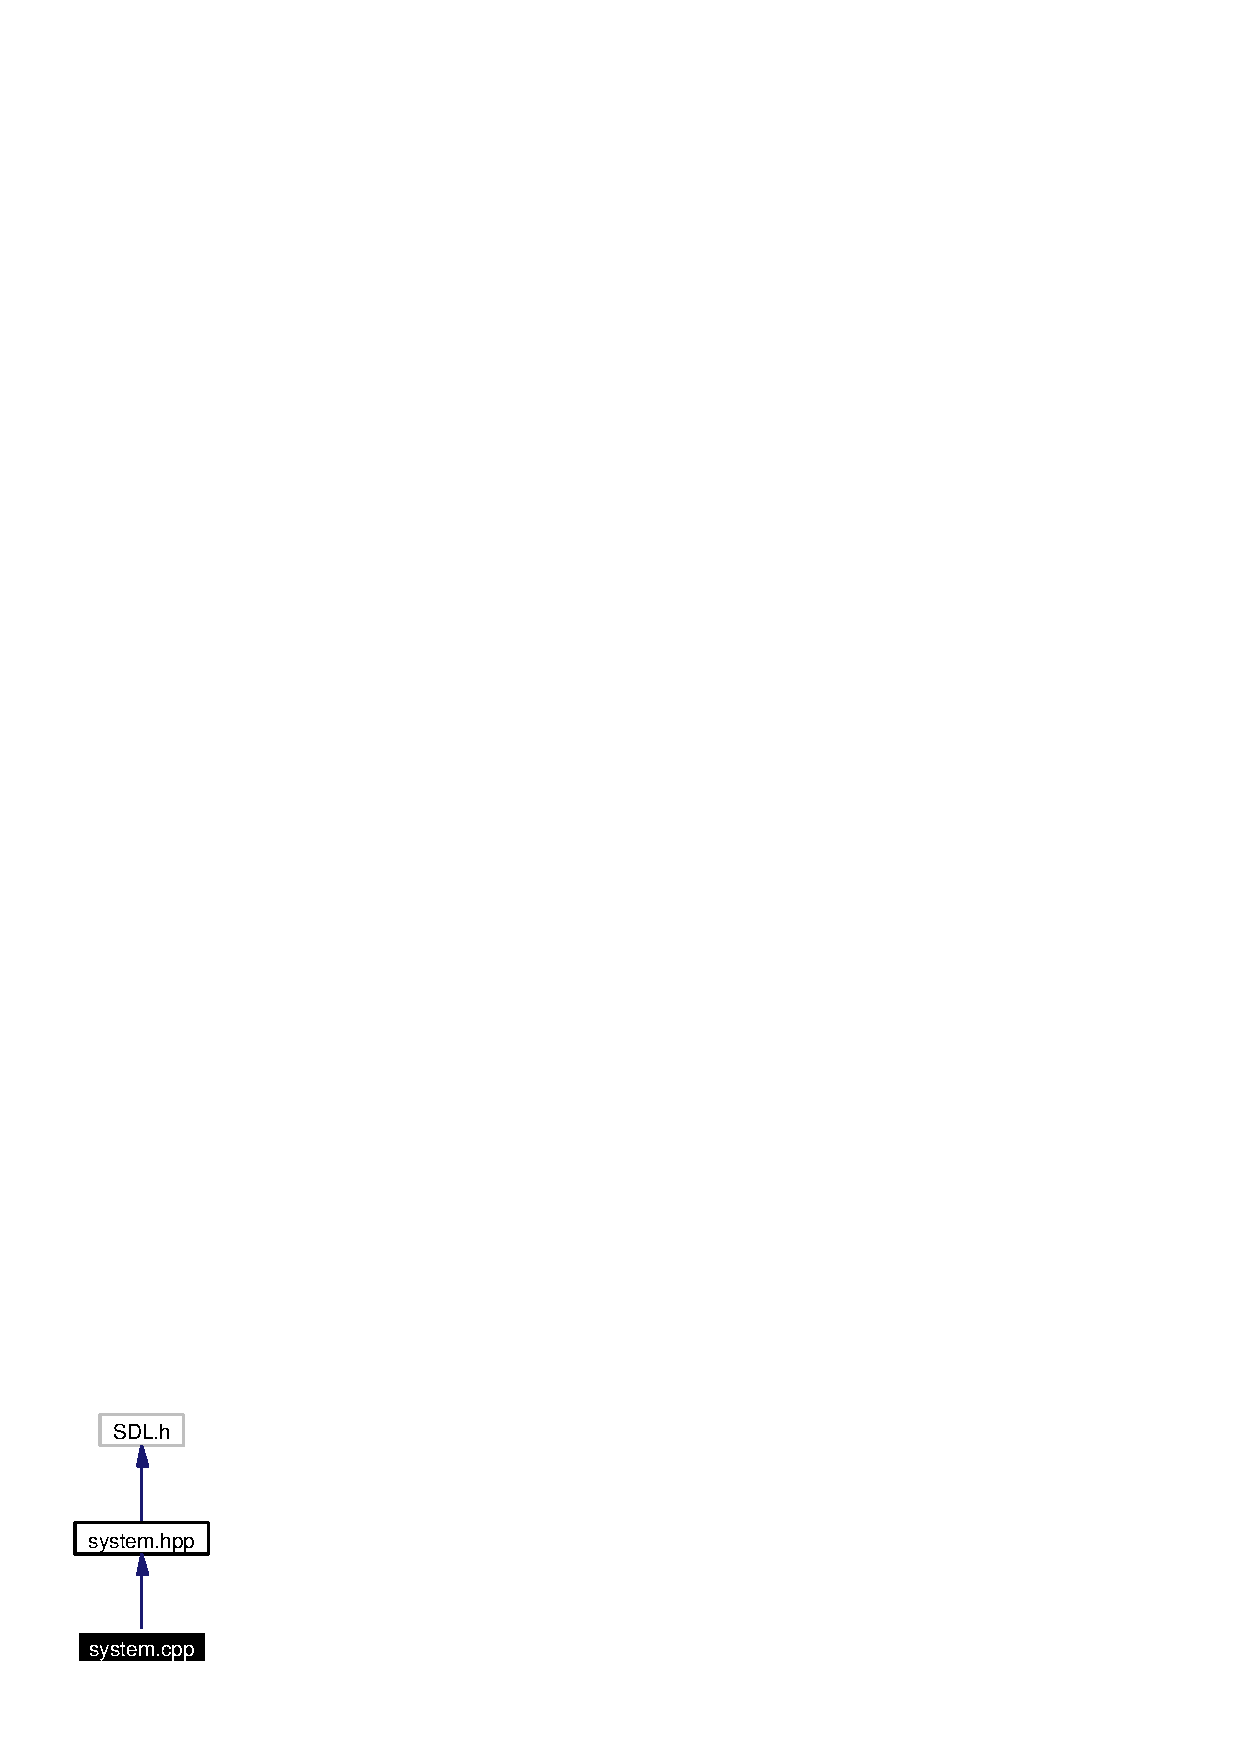
\includegraphics[width=50pt]{system_8cpp__incl}
\end{center}
\end{figure}
\subsection*{Variables}
\begin{CompactItemize}
\item 
bool {\bf main\-Loop\-Enabled}
\item 
bool {\bf sim\-Loop\-Enabled}
\item 
bool {\bf gui\-Loop\-Enabled}
\end{CompactItemize}


\subsection{Variable Documentation}
\index{system.cpp@{system.cpp}!guiLoopEnabled@{guiLoopEnabled}}
\index{guiLoopEnabled@{guiLoopEnabled}!system.cpp@{system.cpp}}
\subsubsection{\setlength{\rightskip}{0pt plus 5cm}bool {\bf gui\-Loop\-Enabled}}\label{system_8cpp_a2}


\index{system.cpp@{system.cpp}!mainLoopEnabled@{mainLoopEnabled}}
\index{mainLoopEnabled@{mainLoopEnabled}!system.cpp@{system.cpp}}
\subsubsection{\setlength{\rightskip}{0pt plus 5cm}bool {\bf main\-Loop\-Enabled}}\label{system_8cpp_a0}


\index{system.cpp@{system.cpp}!simLoopEnabled@{simLoopEnabled}}
\index{simLoopEnabled@{simLoopEnabled}!system.cpp@{system.cpp}}
\subsubsection{\setlength{\rightskip}{0pt plus 5cm}bool {\bf sim\-Loop\-Enabled}}\label{system_8cpp_a1}



\section{src/system.hpp File Reference}
\label{system_8hpp}\index{src/system.hpp@{src/system.hpp}}
{\tt \#include \char`\"{}SDL.h\char`\"{}}\par


Include dependency graph for system.hpp:\begin{figure}[H]
\begin{center}
\leavevmode
\includegraphics[width=50pt]{system_8hpp__incl}
\end{center}
\end{figure}


This graph shows which files directly or indirectly include this file:\begin{figure}[H]
\begin{center}
\leavevmode
\includegraphics[width=342pt]{system_8hpp__dep__incl}
\end{center}
\end{figure}
\subsection*{Classes}
\begin{CompactItemize}
\item 
struct {\bf Graphics\-Data}
\item 
struct {\bf Gui\-Data}
\item 
struct {\bf Input\-Data}
\item 
struct {\bf Physics\-Data}
\item 
class {\bf System\-Data}
\end{CompactItemize}

\section{src/world.cpp File Reference}
\label{world_8cpp}\index{src/world.cpp@{src/world.cpp}}
{\tt \#include \char`\"{}world.hpp\char`\"{}}\par


Include dependency graph for world.cpp:\begin{figure}[H]
\begin{center}
\leavevmode
\includegraphics[width=47pt]{world_8cpp__incl}
\end{center}
\end{figure}

\section{src/world.hpp File Reference}
\label{world_8hpp}\index{src/world.hpp@{src/world.hpp}}
{\tt \#include \char`\"{}SDL.h\char`\"{}}\par


Include dependency graph for world.hpp:\begin{figure}[H]
\begin{center}
\leavevmode
\includegraphics[width=47pt]{world_8hpp__incl}
\end{center}
\end{figure}


This graph shows which files directly or indirectly include this file:\begin{figure}[H]
\begin{center}
\leavevmode
\includegraphics[width=340pt]{world_8hpp__dep__incl}
\end{center}
\end{figure}
\subsection*{Classes}
\begin{CompactItemize}
\item 
class {\bf Rectangle}
\item 
class {\bf World\-Data}
\end{CompactItemize}

\printindex
\end{document}
